
\pdfminorversion=7
\newcommand{\thesistype}{DA} 
\newcommand{\thesislanguage}{en-UK}
\newcommand{\thesistitle}{PD Model Development using Boosted Decision Trees}
\newcommand{\thesistitletranslated}{PD Modelentwicklung mit Boosted Decision Trees}
\newcommand{\titelvorgestellt}{}
\newcommand{\authorname}{Meikee Pagsinohin}
\newcommand{\titelnachgestellt}{, BSc}
\newcommand{\MatrNr}{01327477}
\newcommand{\gender}{F}
\newcommand{\supervisor}{Dr. \textbf{Manuel Lingo}\newline}

\date{August 2023}

\documentclass[11pt,twoside=true]{scrreprt}
\usepackage[utf8]{inputenc}
\usepackage{TUWBUIDADISS}

\raggedbottom 

\begin{filecontents}[overwrite]{\jobname.xmpdata}
\Title{\thesistitle}
\Author{\authorname}
\Language{\thesislanguage}
\Keywords{diploma thesis\sep template\sep LaTeX}
\Publisher{Fachhochschule BFI}
\end{filecontents}

%\usepackage[style=numeric-comp,backend=biber,maxcitenames=2]{biblatex}
%\ExecuteBibliographyOptions{%
%  giveninits=true,maxbibnames=99}%
%\DefineBibliographyStrings{ngerman}{andothers={et\;al\adddot},
%urlseen = {Zugriff am}}
%\addbibresource{Literature.bib}

\usepackage{float}
\usepackage{longtable}
\usepackage{multirow}
\usepackage[normalem]{ulem}
\usepackage{lscape}
\usepackage[toc,page]{appendix}
\usepackage{setspace}
\usepackage{tabularx}
\usepackage{booktabs}
\usepackage{array}
\usepackage[table]{xcolor}
\usepackage{adjustbox}
\newenvironment{conditions}
  {\par\vspace{\abovedisplayskip}\noindent\begin{tabular}{>{$}l<{$} @{${}={}$} l}}
  {\end{tabular}\par\vspace{\belowdisplayskip}}
\newenvironment{conditions*}
  {\par\vspace{\abovedisplayskip}\noindent
   \tabularx{\columnwidth}{>{$}l<{$} @{${}={}$} >{\raggedright\arraybackslash}X}}
  {\endtabularx\par\vspace{\belowdisplayskip}}
\newcolumntype{L}{>{\raggedright\arraybackslash}p{4cm}}
\newcolumntype{R}{>{\raggedright\arraybackslash}p{2cm}}

\bibliographystyle{habbrv}
\usepackage{hyperref}
\usepackage{xcolor}
\hypersetup{
    colorlinks,
    linkcolor={black!50!black},
    citecolor={blue!50!black},
    urlcolor={blue!80!black}
}

\usepackage{acro}
\DeclareAcronym{obv}{
short = {\"obv},
long  = {Österreichische Bautechnikvereinigung},
}

\DeclareAcronym{LZKB}{
short = {LZKB},
long  = {Lebenszykluskosten Brücken},
}

\DeclareAcronym{dt}{
short = {dt.},
long  = {deutsch},
}

\DeclareAcronym{abbv}{
short = {ABBV},
long  = {Ablösungsbeträge-Berechnungsverordnung},
short-plural = {s},
long-plural = {en},
}

\DeclareAcronym{lzk}{
short = {LZK},
long  = {Lebenszykluskosten},
extra = {[\officialeuro{}]},
}



%% Einstellungen für Zeilenumbrüche von Weblinks im url-Paket
%\setcounter{biburllcpenalty}{9000}% Kleinbuchstaben
%\setcounter{biburlucpenalty}{9000}% Großbuchstaben
%% Quelle: https://texwelt.de/fragen/7008/zeilenumbruche-in-bibliografielinks

%% ===== additional settings =============
\setcounter{secnumdepth}{4}
\setcounter{tocdepth}{4}
\sisetup{output-decimal-marker = {,},
range-phrase = --,
group-separator = {~},
per-mode = symbol, 
list-final-separator={ und }}

\graphicspath{{Figures/}}

%% examples for useful shortcuts in German
\newcommand{\zB}{\mbox{z.\,B.}\xspace}
\newcommand{\Name}[1]{\textsc{#1}}

\newcommand{\vKTxv}{\mathbf{v}_1^T\tilde{\mathbf{K}}_{T},_{\xi}\mathbf{v}_1}
\newcommand{\vKTxxv}{\mathbf{v}_1^T\tilde{\mathbf{K}}_{T},_{\xi\xi}\mathbf{v}_1}

%\renewcommand{\thesection}{\arabic{section}}

%% activate for double space between the lines (correction mode) 
%\doublespacing

\begin{document}       		%% start of the document
%\maketitle             		%% places the title with above information

\begin{titlepage}
	\centering
	%
\includegraphics[width=0.5\textwidth]{figures/FHlogo.png}\par\vspace{1cm}
	\vspace{1cm}
	{\scshape\LARGE Masterthesis \par}
	\vspace{1cm}
	{\scshape\Large \par}
	\vspace{1.5cm}
	{\huge\bfseries Predicting the Probability of Default using the Random Forest Algorithm \par}
	\vspace{2cm}
	%{\Large Ausgeführt am Institut für Hochenergiephysik der Österreichischen Akademie der Wissenschaften \par}
	\vspace{2cm}
	%{\Large unter der Anleitung von \par}
	%{\Large\bfseries Dipl.-Ing. Dr.techn. Robert Schöfbeck \par}	
	\vspace{2cm}
	%{\Large durch \par}	
	{\Large\bfseries Meikee PAGSINOHIN \par}	
	\vfill
	{\Large Matrikelnummer: 01327477 \par}

	\vfill

\end{titlepage}


\selectlanguage{english}  	%% for german abstract: ngerman
\chapter*{Summary}
      		%% german abstract (about 1 page)

%\cleardoublepage
\selectlanguage{english} 
\pagestyle{scrheadings} 

%% insert table of contents
\tableofcontents

\chapter{Introduction}
\section{Problem Outline and Significance}

In the financial industry, credit risk is a critical aspect that demands diligent assessment and management. While traditional scoring models like logistic regression have enjoyed popularity for their performance and intuitive explanations, they often fall short in capturing intricate patterns, non-linear relationships of risk factors and handling unexplored forms of information such as unstructured and transactional data. As a result, there is a compelling need for innovative and sophisticated methodologies that can enhance the accuracy and reliability of predicting the \ac{PD}.

By investigating the application of the Random Forest algorithm, the research aims to offer practical insights that can further advance credit risk assessment practices. The findings of this research seek to support financial institutions with a more accurate and adaptable model for assessing credit risk, enabling them to make better informed lending decisions and enhance overall portfolio management. The thesis contributes to the academic discourse by exploring the practical application of the Random Forest algorithm in a real-world financial context. It opens possibilities for further research into the interpretability and transparency of machine learning models in credit risk assessment.

\section{Research Question}

This master thesis addresses two pivotal research questions. Firstly, the study seeks to determine whether a model developed by applying the Random Forest algorithm outperforms a traditional logistic regression model in predicting the \ac{PD} applied to an American mortgage loan portfolio. This comparative analysis aims to provide valuable insights to enhance the accuracy of credit risk assessments. Secondly, the research investigates strategies to overcome the inherent "Black Box" nature of machine learning models, specially focusing on increasing their interpretability. 

\section{Methodology}

The methodology employed in this master thesis is designed to thoroughly assess and compare the predictive performance of the Random Forest algorithm against a traditional logistic regression model in the domain of credit risk assessment. Utilizing an American mortgage loan data set, the research begins with approximating of the default flag, fulfilling the requirement stated in \ac{CRR} Article 178(1). Then, the data is preprocessed to address missing values and outliers. A portion of the data set is allocated for training the logistic regression and Random Forest models. The Random Forest model is additionally optimized through hyperparameter tuning to enhance its predictive capabilities. The models are then evaluated on separate testing and out-of-time data sets, employing key performance metrics such as the area under the Receiver Operating Characteristic curve, Gini coefficient, F1-score and confusion matrix. Additionally, the thesis incorporates an exploration of interpretability-enhancing techniques. The combined methodology ensures a comprehensive investigation into the strengths and limitations of these predictive modeling approaches.

\section{Structure}

The structure of this master thesis is split into two parts: Theory introduction and empirical research. 

Chapter \ref{ch:CR} introduces the foundational concepts of credit risk and the regulatory framework. Traditional credit risk models, such as logistic regression, are explored in Chapter \ref{ch:TM}, alongside other models like linear regression and external ratings. Chapter \ref{ch:AM} describes advanced models, including decision trees and neural networks. The modeling process is detailed in Chapter \ref{ch:MP}, covering data preparation, logistic regression and Random Forest modeling steps. Validation methods, including out-of-sample and out-of-time validation, are discussed in Chapter \ref{ch:VL}, accompanied by performance evaluation metrics and stability tests. Chapter \ref{ch:IP} addresses the crucial aspect of interpretability in machine learning models, discussing its importance and presenting methods for interpretability analysis. 

Chapter \ref{ch:RE} delves into the specifics of the data used and the results obtained, utilizing Freddie Mac's Single Family Loan-Level Data set. It covers data quality, limitations, sample creation, data preparation, variable selection and the modeling process for both logistic regression and Random Forest approaches. Validation and comparison metrics are presented, followed by a detailed exploration of interpretability through global and local interpretations, individual decision trees, Partial Dependence Plots and Individual Conditional Expectation plots. 
This well-structured framework ensures a systematic and insightful investigation into the research questions.

\chapter{Credit Risk}
\label{ch:CR}

\section{Credit Risk management}
Part of the daily business of a financial institution is the credit risk assessment of existing and new customers. The result is used to decide if they want to decline or grant a credit application and, among other things, to set the required regulatory capital. Credit risk assessment is performed during the whole lifetime of an exposure. It starts with the approval of a transaction and is continuously monitored afterward. Corporate clients usually need to submit financial reports regularly, which are then analyzed by their bank advisor and credit analyst, while it is done automatically for retail customers via behavior scoring. 

The information used during the application scoring is limited because the applicant mainly provides it at the start of a new contract. It generally covers variables about their financial health, e.g., income and outstanding debt. For the behavior scoring model, internal historical data is used, for example, the borrower's payment history and credit utilization. The behavior model generally shows a better predictive performance than the application model. If a decline in financial health or behavior rating is detected, the bank may try to decrease the overdraft limit to regulate the credit risk. In the case of delayed payments, the early collection process starts, where affected customers are contacted and an alternative payment plan will be negotiated. If all interventions fail, defaulted exposures may be sold or outsourced to collection companies for further processing, like the sale of collateral. \cite[p.~7]{Witzany:2017}

\section{Default Rate and Probability of Default}
\label{sec:dr_pd}
A critical risk measure is the \acl{PD}, which is an estimate of the likelihood of a borrower failing to pay back their financial obligations in a given time period. Depending on the analyzed portfolio, the expected number of defaults can vary. In the corporate segment, individual defaults might already be seen as an indicator of a bank's failing credit assessment process and decision. In contrast, a higher number of defaults can be expected in the retail sector. On the contrary, profit is generated if the income gained from non-defaulted customers covers the loss from the defaulted portion of the portfolio. \cite[p.~2]{Witzany:2017}

\medskip
In the Capital Requirements Regulation (\ac{CRR} Article 178(1)), the definition of default is stated as:

\begin{quote}

A default shall be considered to have occurred with regard to a particular obligor when either or both of the following have taken place:
\begin{itemize}
\item[(a)] the institution considers that the obligor is unlikely to pay its credit obligations to the institution, the parent undertaking or any of its subsidiaries in full, without recourse by the institution to actions such as realising security;
\item[(b)] the obligor is more than 90 days past due on any material credit obligation to the institution, the parent undertaking or any of its subsidiaries. Competent authorities may replace the 90 days with 180 days for exposures secured by residential property or SME commercial immovable property in the retail exposure class, as well as exposures to public sector entities. The 180 days shall not apply for the purposes of point (m) Article 36(1) or Article 127.

\end{itemize}

In the case of retail exposures, institutions may apply the definition of default laid down in points (a) and (b) of the first subparagraph at the level of an individual credit facility rather than in relation to the total obligations of a borrower.

\end{quote}

A time period has to be defined in which a default event is observed, commonly a one-year observation window is used. If the customer does not default during this period, the \emph{Default\_12M} flag remains at 0. If a default occurs within the first 12 months after the start of the contract or reference point, the flag is set to 1. Notably, even if a default happens after 12 months, the flag remains at 0. An illustration is visible in Figure \ref{fig:cr_timeperiod}. The default rate per category (e.g., month, rating grade) is then calculated as the number of defaults divided by the total number of customers (Eq. \ref{eq:cr_dr}).

\begin{equation}
DR_{i} = \frac{d_{i}}{n_{i}} \label{eq:cr_dr}
\end{equation}
where:
\begin{conditions}
 d_{i}  & number of defaults in class i \\
 n_{i}  & number of observations in class i
\end{conditions}

\begin{figure}[H]
	\centering
	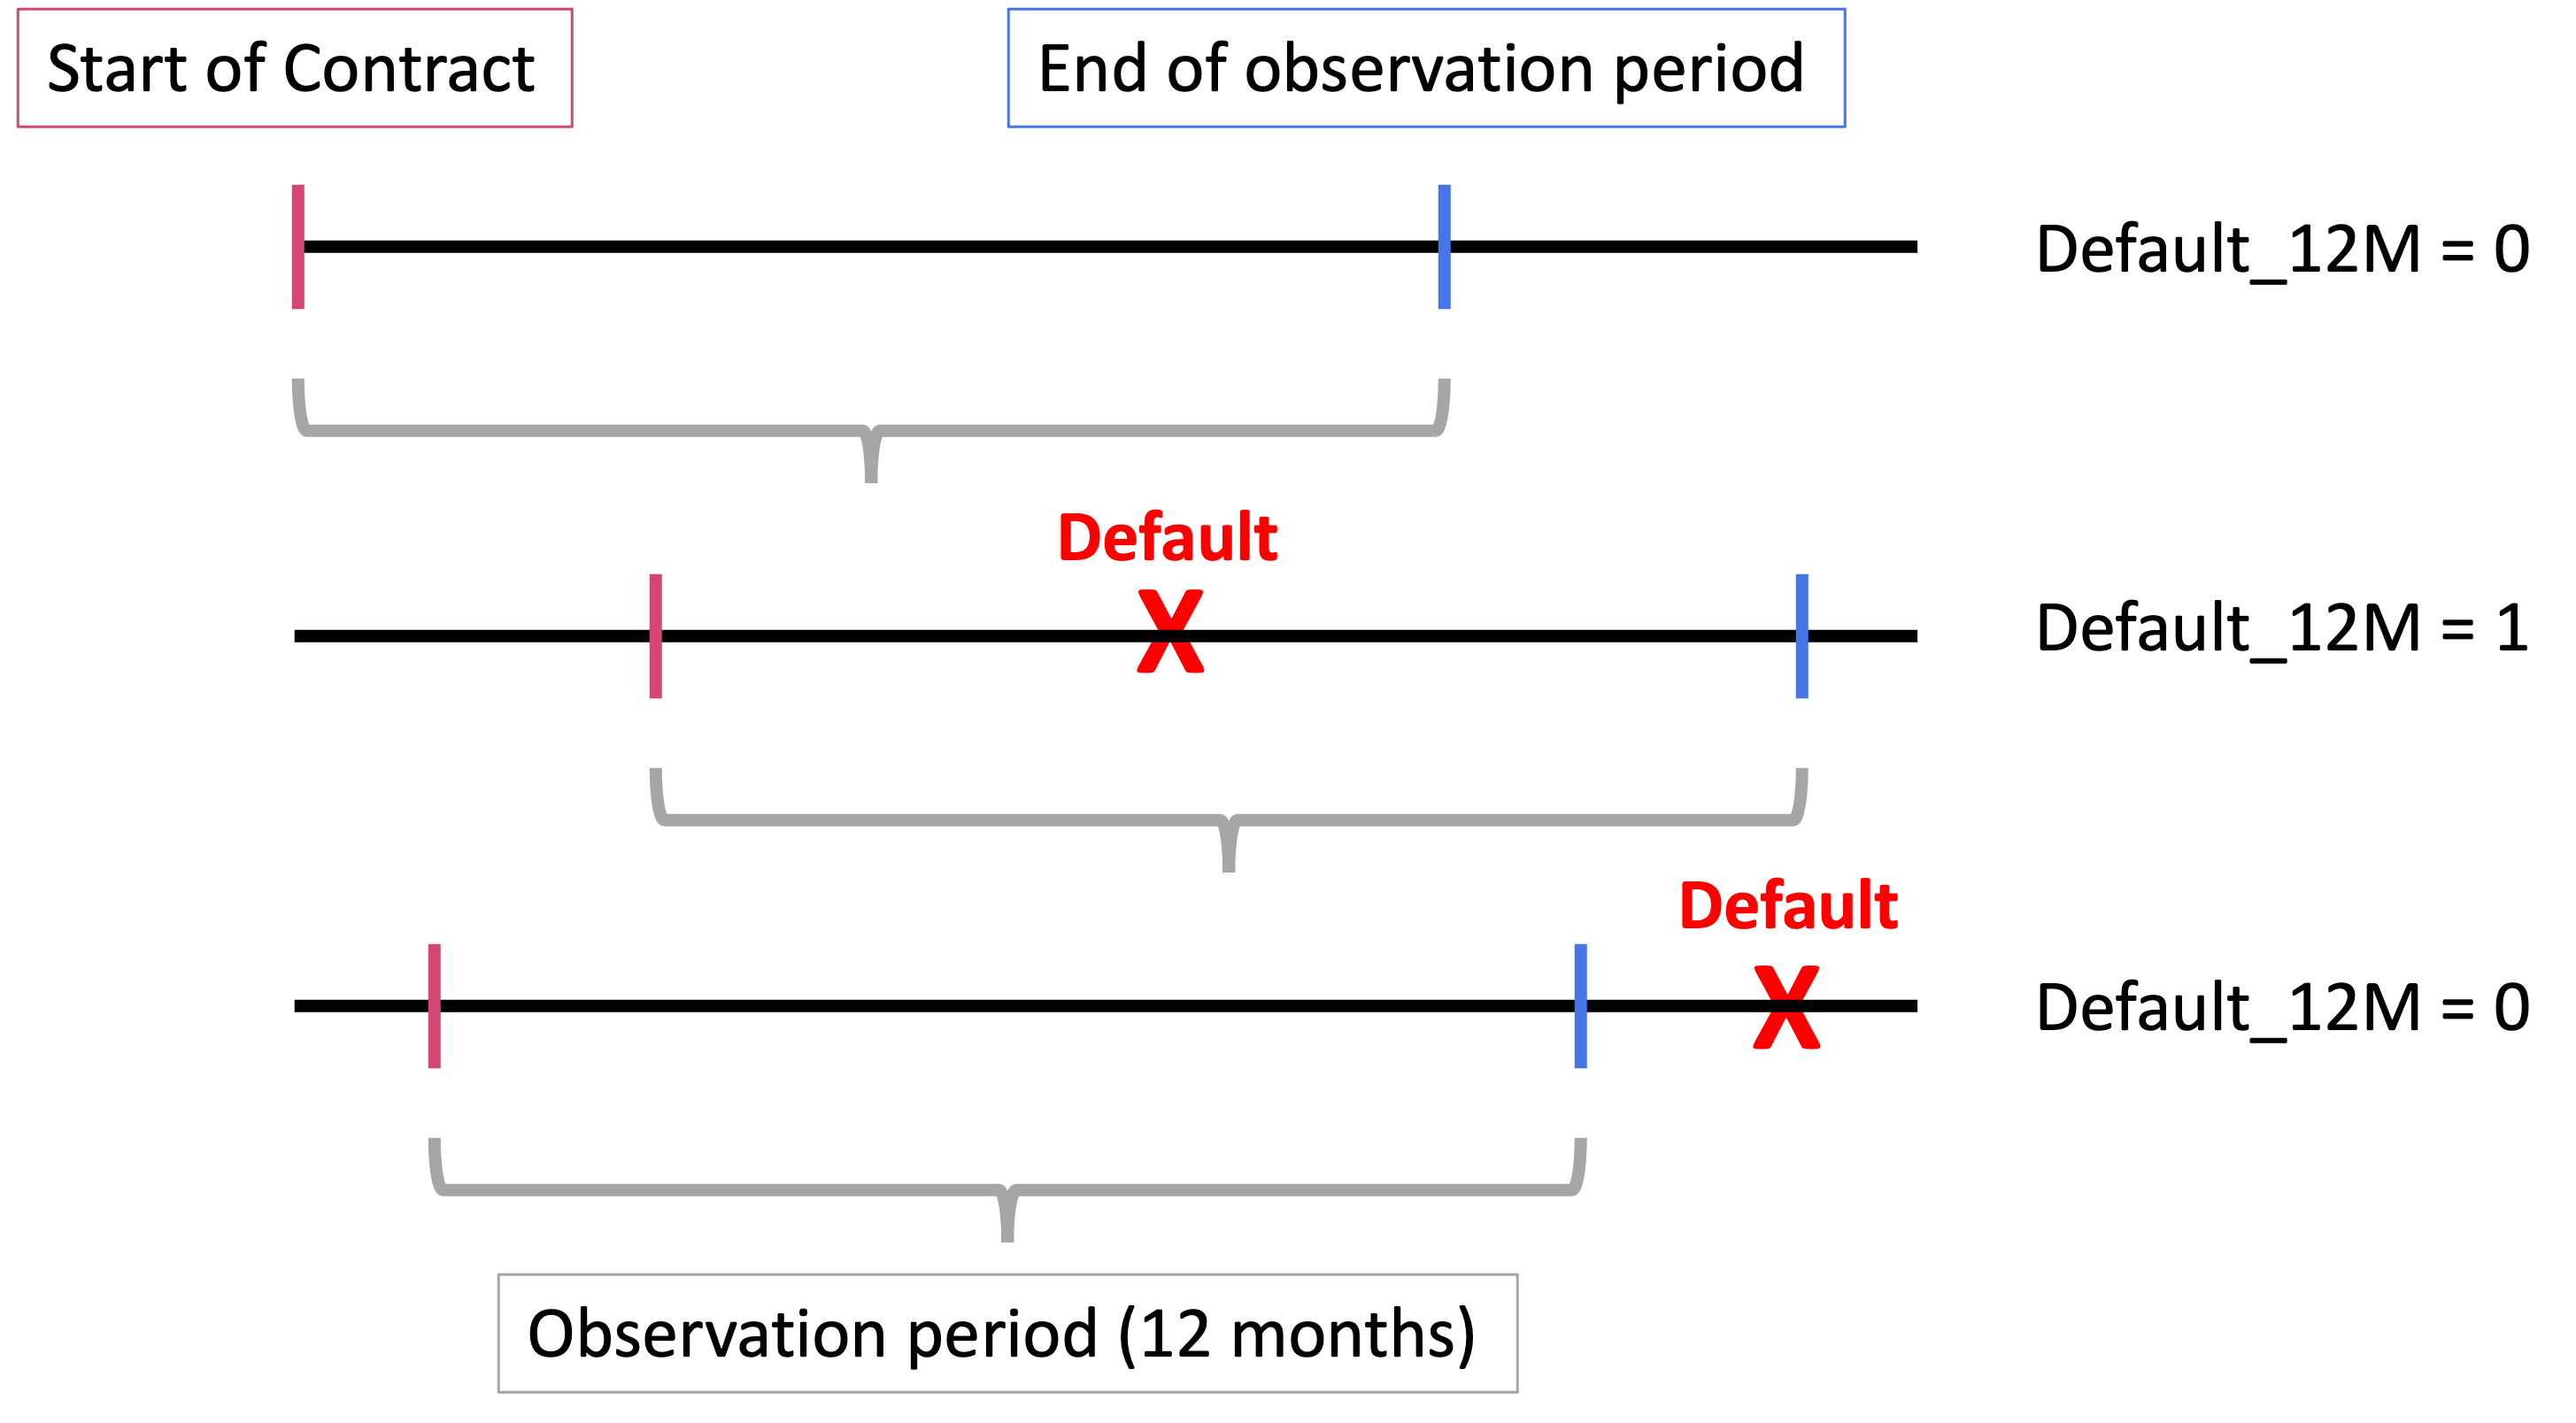
\includegraphics[width=.625\textwidth]{./CR__ObservationPeriod.png}
    \caption{Observation period, Setting of Default flag}
    \label{fig:cr_timeperiod}
\end{figure}

\section{Regulatory Framework}

\subsection{History of Regulatory Framework}

The Basel Committee on Banking Supervision, comprising 45 institutions from 28 jurisdictions since its establishment in 1945 with its headquarters in Basel, Switzerland, is dedicated to defining a high standard for risk management and internal controls and establishing a risk-sensitive calculation process of the regulatory capital for banks worldwide. The Basel Capital Accord, also known as Basel I, was first published in 1988 and set the minimum capital adequacy ratio at 8\%. Basel II, the New Capital Accord, was introduced in 2004 and implemented the three pillars encompassing the minimum capital requirements, supervisory review and market discipline. At the end of 2010, a new reform called Basel III was approved to address the variability in reported risk-weighted capital ratios during the global financial crisis, incorporating stricter regulations for the capital calculation approaches and setting a revised leverage ratio and output floor. \cite{BCBS:2023}

\subsection{Credit Risk Regulatory Capital}

The credit risk capital requirement calculation was significantly improved compared to the First Capital Accord. The total loss of a bank is split into expected and unexpected loss. The former should be covered by revenue; for the latter, a bank must allocate an appropriate level of capital. In the original approach, each exposure was assigned to one of four risk categories and then a multiplier ranging from 0-100\% was applied. Regulations now allow the \ac{SA}, Foundation or Advanced Internal Rating Based (IRB-F, IRB-A) Approach. 

The \acl{SA} defines five risk buckets for calculating regulatory capital and it also allows the use of external ratings. For the \ac{IRB} approach, internal models estimate input parameters of the regulatory formulas, which then result in risk weights for each exposure used in the calculation of the regulatory capital. The IRB-F approach only permits the estimation of the PD. In contrast, for the IRB-A approach, the risk parameters Loss Given Default, Exposure at Default, Conversion Factor and Effective Maturity are additionally derived from internal models. While the corporate segment allows for both IRB-F and IRB-A approaches, the retail portfolio is limited to the IRB-A approach. \cite[15-17]{Witzany:2017} 

\subsection{Machine Learning for IRB models}
The integration of advanced machine learning models in the banking industry is in its early stages, as financial institutions struggle with uncertainties regarding the application of requirements outlined in the \acl{CRR} and other legal frameworks such as the \ac{GDPR} and the Artificial Intelligence (AI) Act. Notably, the AI Act designates credit scoring as a high-risk use case, given its potential impact on an individual's access to financial resources. Within the banking sector, machine learning models find additional application in areas like fraud detection, transaction clustering and real-time monitoring of payments. Decision trees are commonly utilized in the development of \ac{IRB} models for variable selection, clustering processes and as model challengers in subsequent validation. 

Financial institutions encounter challenges related to overfitting and interpretation of machine learning models, compounded by a shortage of credit risk analysts equipped with the necessary skills to navigate these complexities. Overfitting issues are particularly pronounced in low default portfolios, where the training of advanced models necessitates extensive data for robust outcomes. Credit analysts with expertise in overcoming these challenges, including hyperparameter tuning, interpretation methods and evaluating output stability and bias, are scarce. Another significant barrier lies in the acceptance of more complex models, requiring a solid understanding from all participants, especially senior management, stakeholders and the sales force. Additionally, one of the objectives of employing machine learning models is leveraging unstructured data; however, \ac{GDPR} Article 9 prohibits the use of personal data, necessitating additional efforts to analyze the compliance of input information. Despite these challenges, the ongoing integration of advanced machine learning models in the banking sector signals a transformative shift, with the need for collaborative efforts to navigate regulatory requirements, enhance analytical capabilities and foster a deeper understanding among key stakeholders.\cite[pp.~4-7, 9, 11, 13]{EBA:2023}

\chapter{Traditional models}
\label{ch:TM}

To estimate a PD model, different types of models varying in complexity are available:

\begin{enumerate}
  \item Statistical Models: This type utilizes historical data for the estimation process. Techniques such as logistic regression, survival analysis and machine learning algorithms are used to predict default events and analyze contributing risk factors.
  \item External Rating Models: Rating agencies develop models that assign credit ratings to borrowers. These models consider various factors, e.g., financial statements and macroeconomic conditions, to evaluate creditworthiness. These types of PD models are only available for a limited portion of borrowers. 
  \item Expert Judgment: In cases where historical data is limited or only a low number of default events is available, expert judgment will become the most relevant method. Experienced credit analysts rely on their expertise and industry knowledge to estimate the PD based on qualitative factors, market conditions and client information.
\end{enumerate}

In practice, a substantial portion of the banking sector employs a combination of multiple types of models in their credit risk assessment.

\section{Logistic regression}
Logistic regression is one of the banking industry's most commonly used statistical models. In the logit model, the log odds are modeled as a linear function, given in Equation \ref{eq:tm_logodds}. The right side, also called  linear predictor, result in a model score, which can take any negative or positive value. Equation \ref{eq:tm_logodds} can be re-formulated to calculate the \ac{PD}, yielding Equation \ref{eq:tm_prob}, which presents the logistic function that confines the probability within the range of 0 to 1. Therefore, a high model score means a lower \ac{PD} and vice versa. \cite[283]{Kuhn:2013}

\begin{figure}[H]
\begin{minipage}{.5\textwidth}
	\begin{align}
	log (\frac{PD}{1 - PD}) = \sum_{i=1}^{n} \beta_{0} + \beta_{i} \times x_i \label{eq:tm_logodds}\\
	PD = \frac{1}{1 + e^{-(\sum_{i=1}^{n} \beta_{0} + \beta_{i} \times x_i)}} \label{eq:tm_prob}
	\end{align}
\end{minipage}%
\begin{minipage}{.5\textwidth}
	\centering
	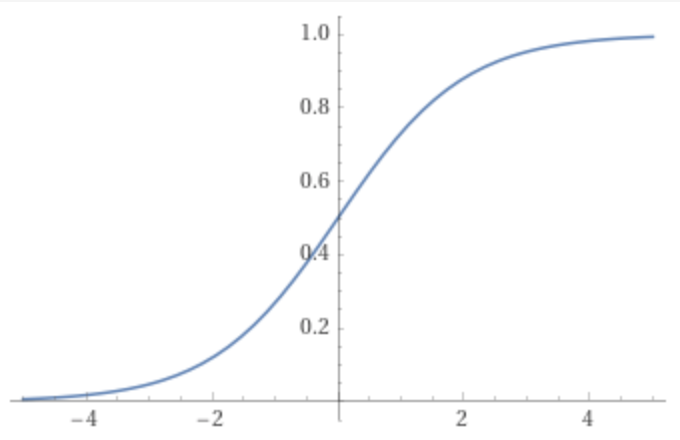
\includegraphics[width=.5\textwidth]{./TM__logistic_func.png}
\end{minipage}
    \caption{Logistic Function}
    \label{fig:tm_logfunc}
\end{figure}

\section{Other Models}

\subsection{Linear regression}
During the linear regression, the algorithm estimates a linear relationship between the default variable, which assumes either the value 0 (non-default) or 1 (default), and explanatory variables, which can be continuous and categorical independent variables, such as income, employment duration and profession. In ordinary least squares linear regression, the goal is to minimize the sum of squared differences between observed and predicted values, with model coefficients determined by Equation \ref{eq:tm_linreg}. The minimization problem is successful, if all explanatory variables are linear independent and thus, correlation between variables have to be reduced. Disadvantages of this method are that the model may output non-logical results, like negative values or a PD over 100\%, and its limitation in capturing non-linear relationships. \cite[pp.~105, 108-109]{Kuhn:2013}

\begin{equation}
\hat{\beta} = (X^T X)^{-1} X^T y \label{eq:tm_linreg}
\end{equation}
where:
\begin{conditions}
\hat{\beta} & Vector of model coefficients \\
X & Matrix of explanatory variables \\
y & Vector of default variable
\end{conditions}

\subsection{External Ratings}
Scorings of corporate clients are usually performed mainly by a credit analyst and only partly automated due to the low number of default events and the type of information available. External ratings may be used if the financial institution needs more resources to develop and maintain internal models. The most known rating agencies are Standard \& Poor, Moody's and Fitch. They provide ratings for a wide range of corporations since most companies request a rating before a sale or registration of a debt issue. 

An analyst will use their financial statements of the last few years and additional information to derive a rating, which is then discussed in a rating committee. Afterward, the corporation is informed about its rating and the corresponding factors and given the opportunity to respond; finally, the ratings will be published. A disadvantage of external ratings observed in the past is the conflict of interest since the company mainly pays the ratings. It is suspected that good ratings were related to high fees, visible during the financial crisis, where many structured bonds with high scorings deteriorated unexpectedly. \cite[pp.~34-36]{Witzany:2017}

\chapter{Machine Learning Models}
\section{Overview}

\section{Decision Trees}
Classification trees are used to separate the categories (default, non-default) as best as possible using explanatory factors. The split is determine by maximising the homogeneity of the resulting subgroups (branch). For numeric variables, the algorithm calculates the measure for each possible threshold, while for categorical variables, it determines the value for each possible split. This step is repeated until a stopping condition is met and the final subgroup is called leaf. To avoid overfitting, the Decision Tree may be "pruned", where some branches are removed. The preliminary decision tree is applied on a separate data set, i.e. the validation sample, and to improve its performance, redundant splits are cut off. An example of a decision tree and the pruning process is visible in Fig. \ref{fig:ml_dectree}. A Separate validation should then be performed on a third test data set, since the validation sample became part of the modelling process. 

\begin{figure}[H]
	\centering
	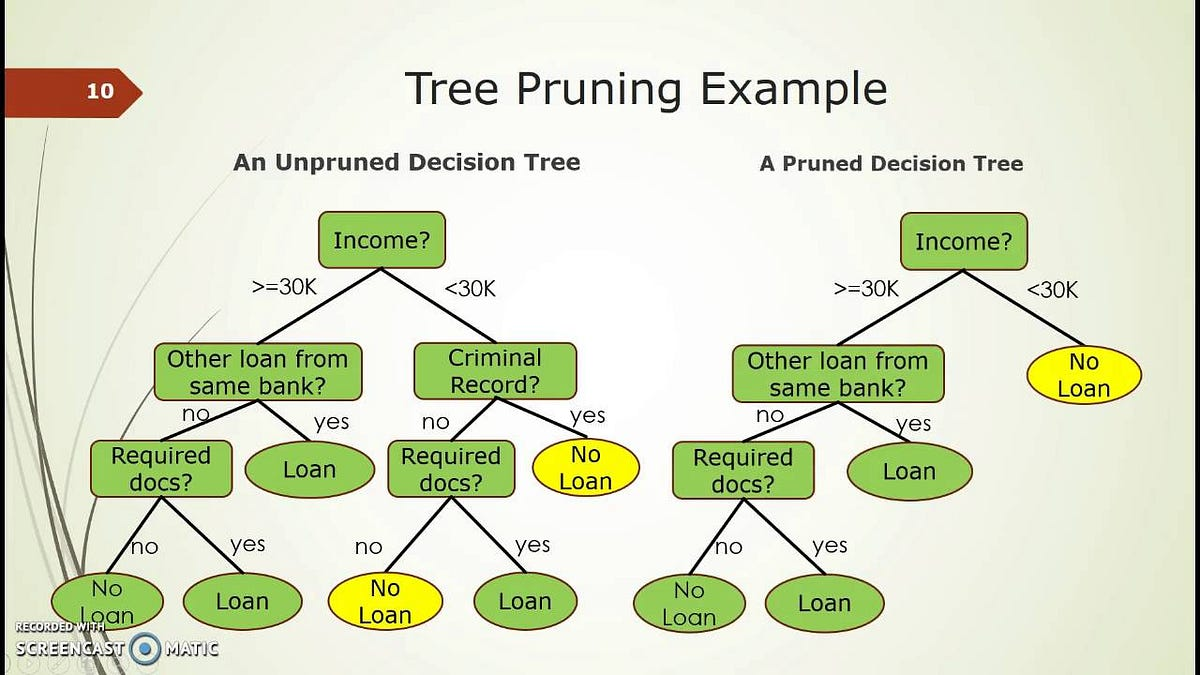
\includegraphics[width=0.625\textwidth]{./ML__DecTree.jpg}
    \caption{Decision Tree incl. Pruning}
    \label{fig:ml_dectree}
\end{figure}

Examples for stopping conditions are that the resulting subgroups are homogeneous, no significant improvement is detected, the minimum leafsize is reached, maximum splits are performed or maximum depth of the tree is achieved. The estimated PD is the average default rate per leaf and each terminal node can be classified into default or non-default using a defined threshold. Popular statistics to measure the homogeneity are Gini index, Kolmogorov-Smirnov statisic or Entropy index. The Gini index assumes a value between 0 and 1, where 0 means complete purity, 0.5 represents an equal distribution of all classes and 1 shows a random distribution across all classes. The formula is given in \ref{eq:ml_gini}. Decision trees usually perform worse than logistic regression models and are rather used to assess the best variables or segmentation possibilities. 

\begin{equation}
GINI = \sum_{i=1}^{n}  p_i \times (1 - p_i) \label{eq:ml_gini}
\end{equation}
where:
\begin{conditions}
 n  	& number of unique classes in variable \\
 p_{i}  & proportion of observations in class n
\end{conditions}

\subsection{Boosted Decision Trees and Random Forests} 
Boosted Decision Trees (BDT), also known as Gradient Boosted Decision Trees combine decision trees with boosting techniques to achieve higher predictive performance. This algorithm iteratively build decision trees, placing more weight on misclassified observations in each iteration, resulting in a strong ensemble model, seen in Fig. \ref{fig:ml_bdt}. BDT are able to capture complex interactions and non-linear relationships in PD modelling. 

\begin{figure}[H]
	\centering
	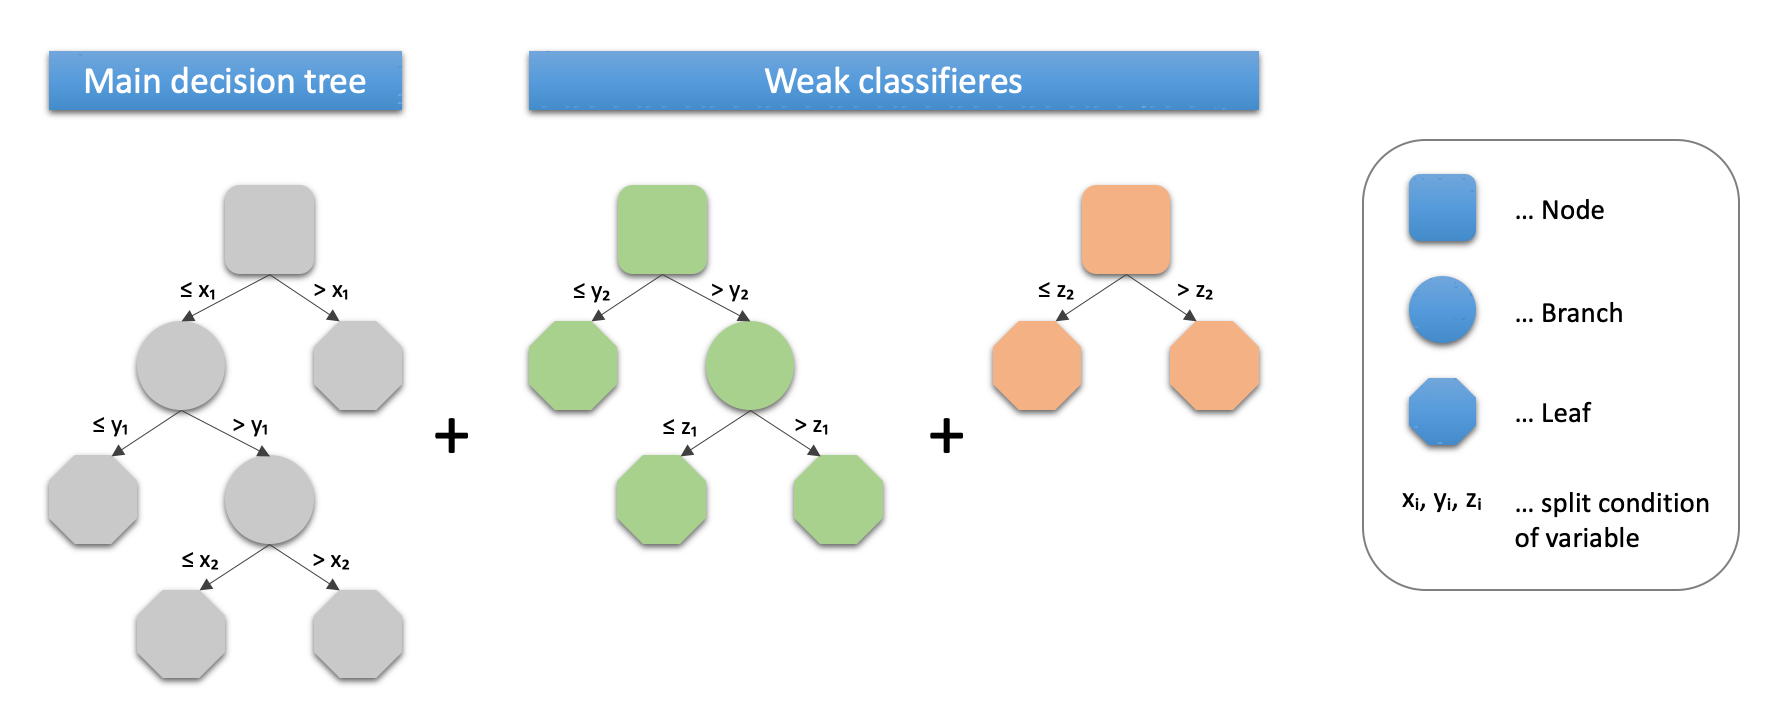
\includegraphics[width=0.625\textwidth]{./ML__BDT.png}
    \caption{Boosted Decision Tree}
    \label{fig:ml_bdt}
\end{figure}

Random forests are an ensemble learning method that combines multiple decision trees to make predictions. However, unlike boosted decision trees, random forests build each tree independently, without sequential corrections (Fig. \ref{fig:ml_ranforest}). This approach reduce the risk of overfitting and the variance of predictions. Random forests are known for their robustness, scalability, and ability to handle high-dimensional data.

\begin{figure}[H]
	\centering
	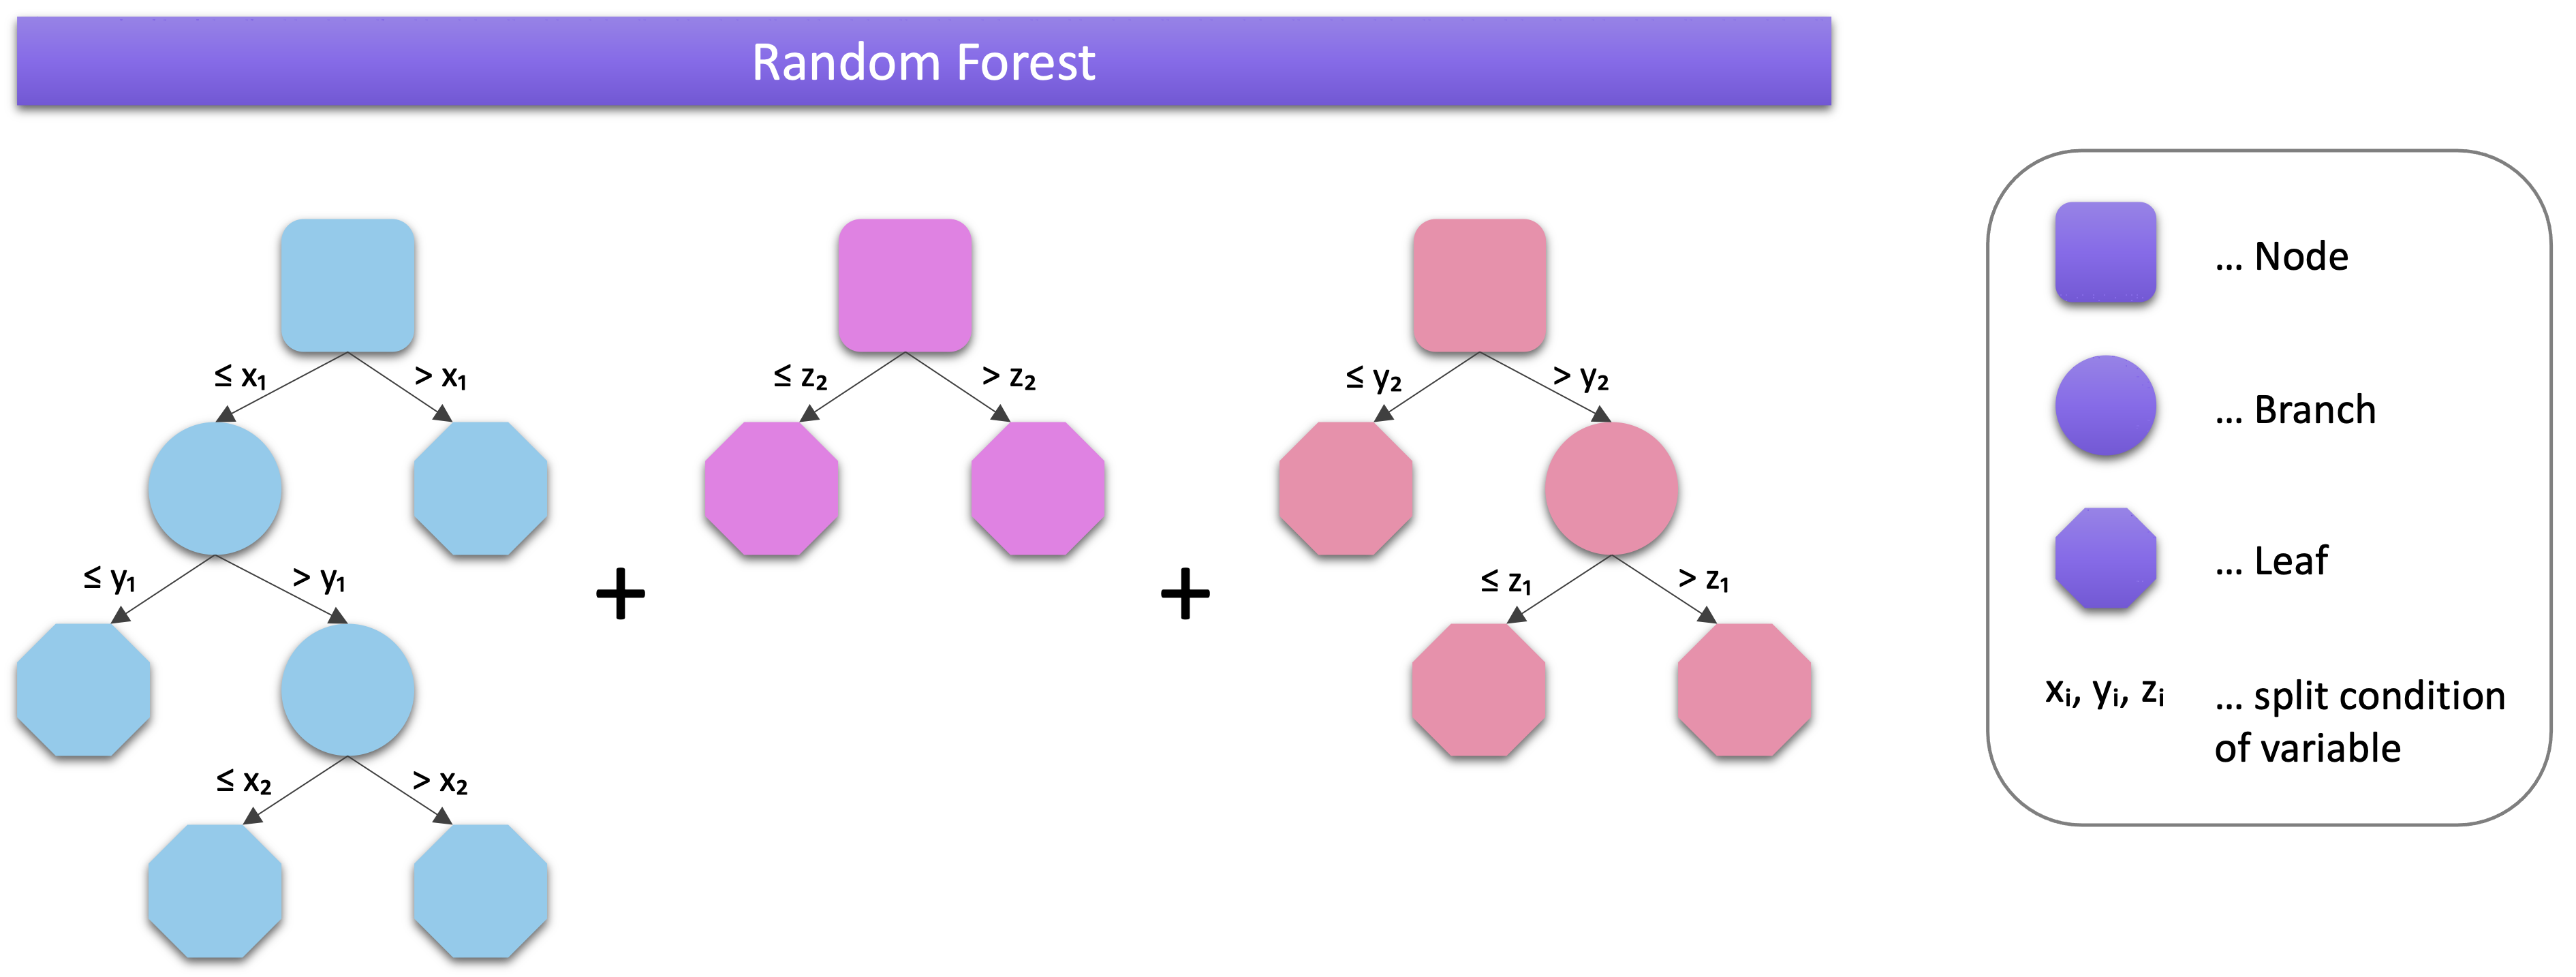
\includegraphics[width=0.625\textwidth]{./ML__Random_forest.png}
    \caption{Random Forest}
    \label{fig:ml_ranforest}
\end{figure}

\section{Other models}

\subsection{Neural Networks}
Neural networks, inspired by the structure and function of the human brain, can learn intricate patterns and nonlinear relationships in data. They consist of multiple layers of interconnected nodes, also called neurons, where each neuron is assigned a simple computation and use activation functions to pass along a value. The result of the model is a numerical or classification value. Commonly used activation functions are logistic function, threshold function or tangent hyperbolic function, listed in Eq. \ref{fig:ml_logfunc} - \ref{fig:ml_tanhfunc}. 

The first and last layer is called the input and output layer respectively, and the layers in-between are hidden layers. An illustration is visible in Figure \ref{fig:ml_neurnet}. Due to the virtually endless possibility of configurations, there is a possibility of over-parametrization, especially with increasing number of hidden layers and nodes, also called deep neural networks. With the ongoing advancements in computational power and data collection capabilities, neural network algorithms have become highly successful in various AI domains.

\begin{figure}[H]
	\centering
	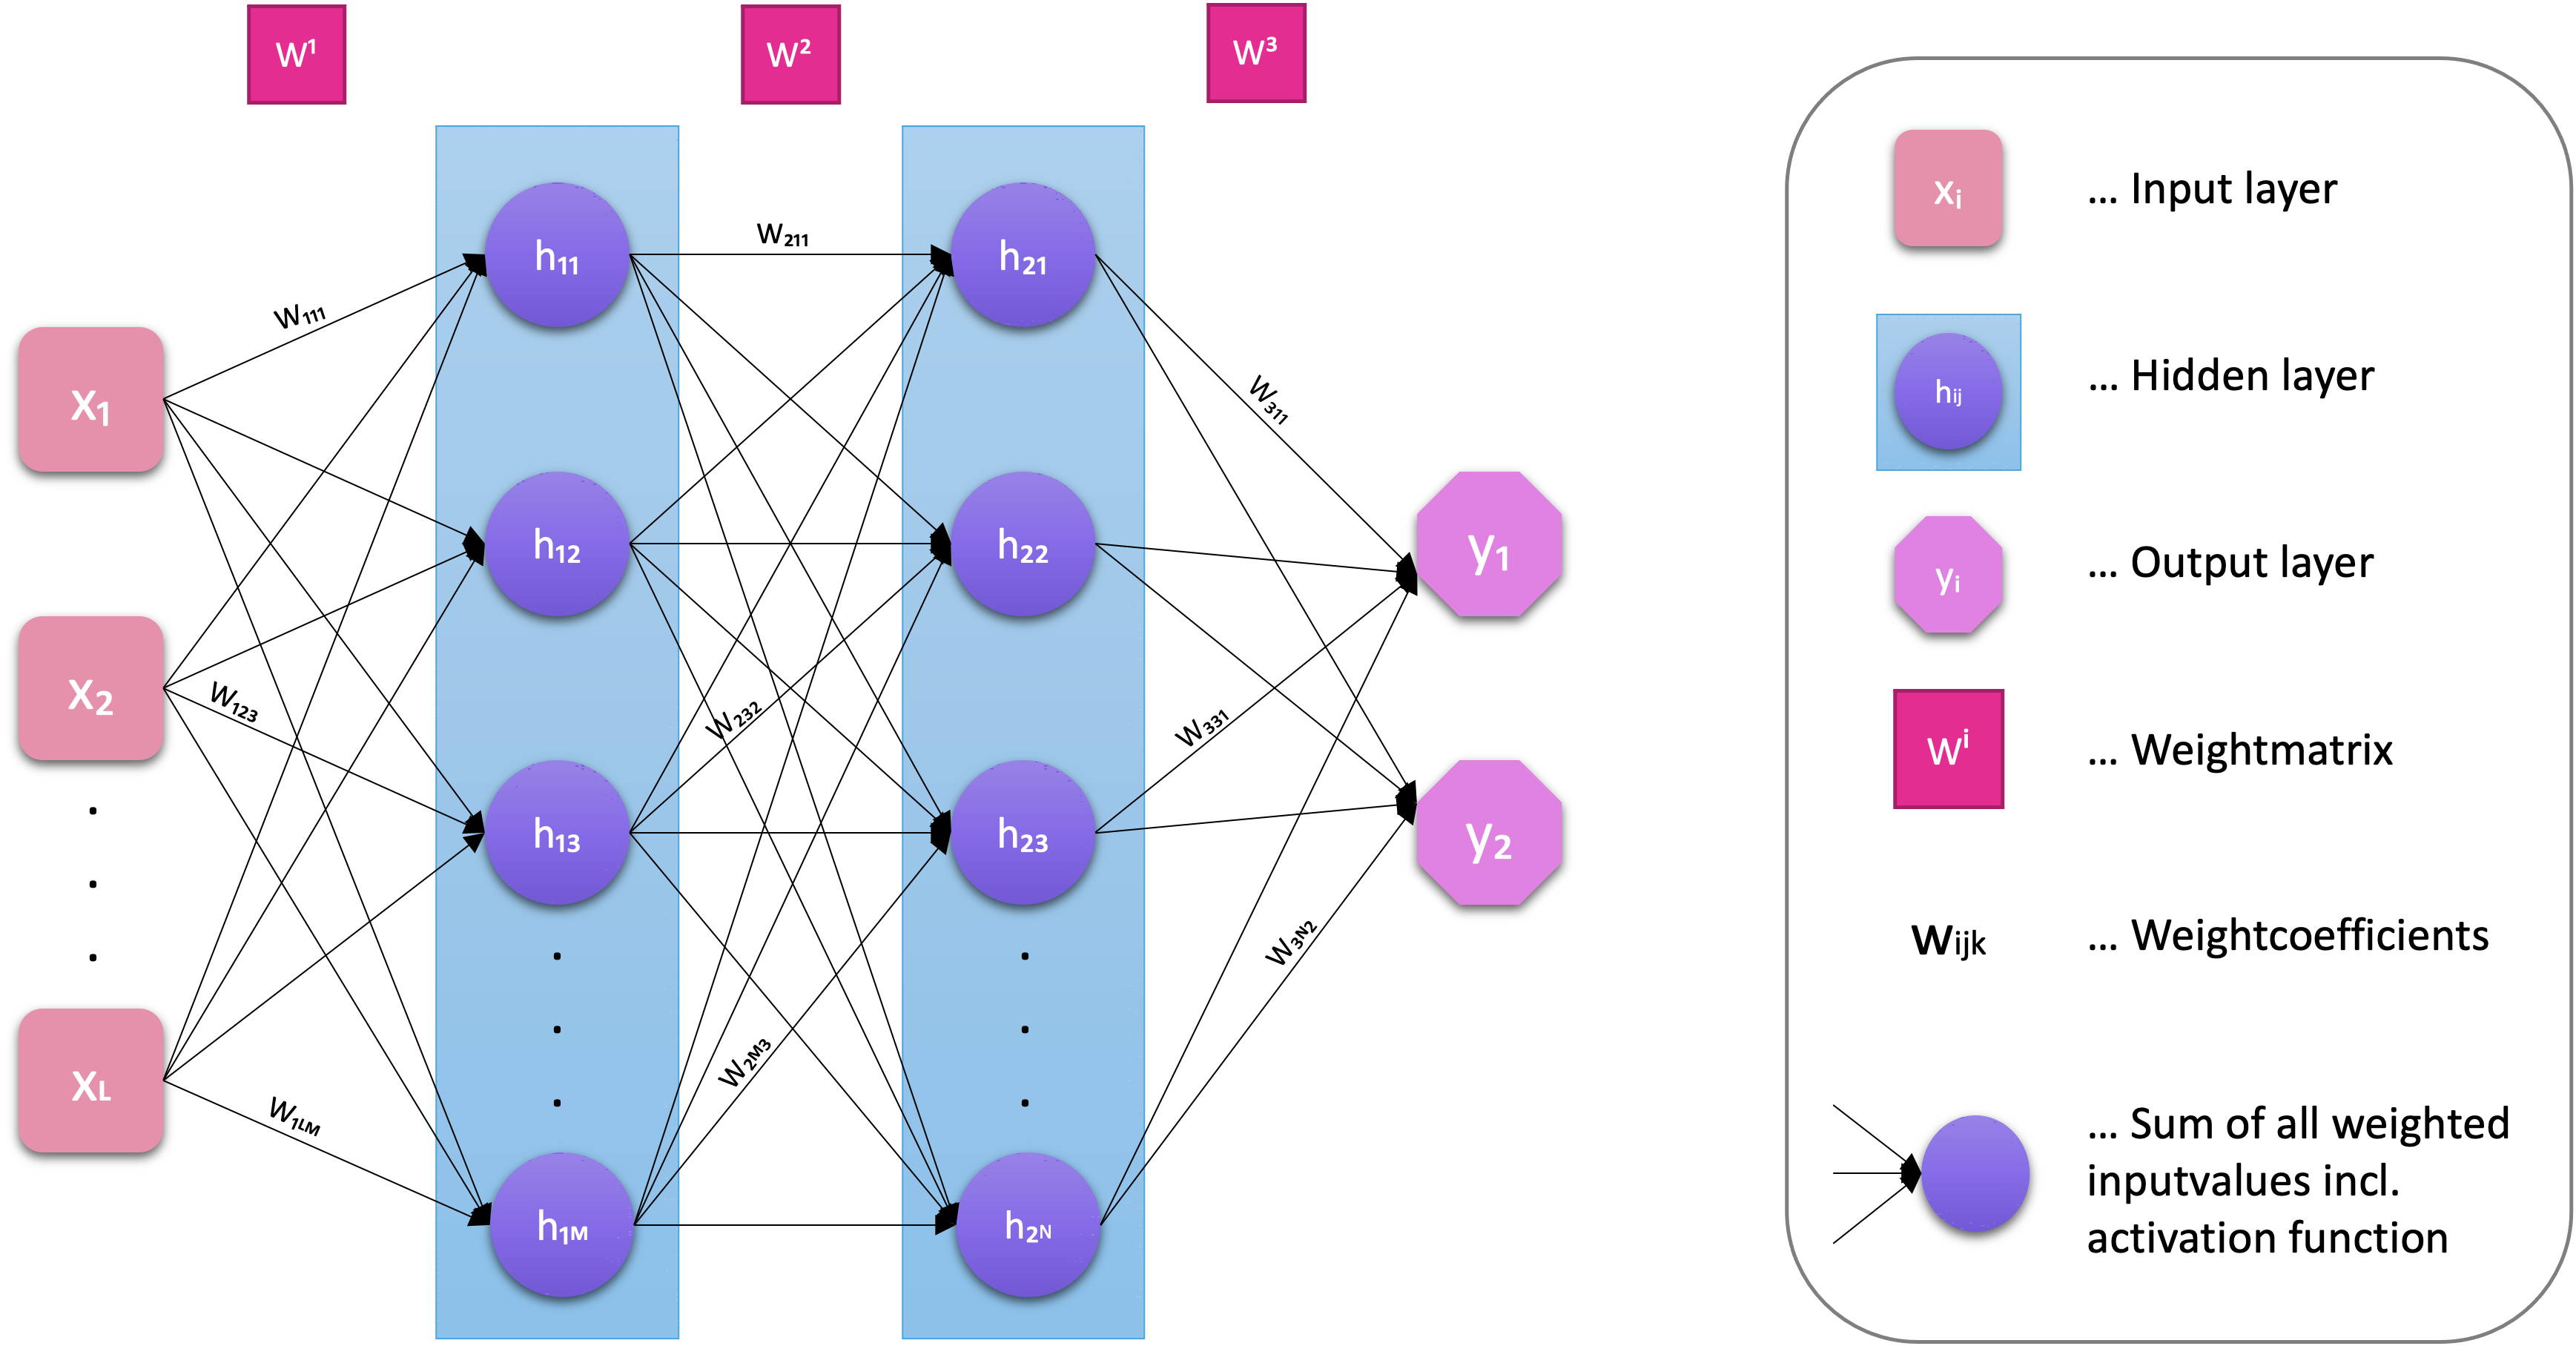
\includegraphics[width=0.625\textwidth]{./ML__MLP.png}
    \caption{Neural Network}
    \label{fig:ml_neurnet}
\end{figure}

\subsection{k-Nearest Neighbour}
\label{sec:kNN}
Using a data set with explanatory factors and known default events, the unknown PD of a new data entry can be determined by taking the nearest data points determined via their risk factors and calculating the average default rate of the new data point. For the definition of distance the Euclidean metric or Manhattan Distance as defined in formula \ref{fig:ml_eucldist} and \ref{fig:ml_manhdist} can be used. The Euclidean distance measures the straight-line distance between two points, while the Manhattan distance is the sum of the absolute differences between two points in a space, where it is only allowed to move along coordinate axes. The number of nearest neighbours k is a hyper-parameter. Advantages of this model is the simple approach and the possibility to dynamically update new and outdated data entries and, if k is set as a low number, individual scorings can be viewed manually by a credit analyst. 

\subsection{Ensamble models}

\chapter{Modeling process}
\label{ch:MP}

\section{Data Preparation}
\label{sec:dataprep}
Explanatory factors can be split into numerical, categorical and indicator variables. Within the corporate segment, these risk factors mostly take the form of numerical variables, such as financial ratios and macroeconomic conditions. The retail sector typically involves categorical factors, including profession, marital status and residential status. Even numerical values like age or employment duration often undergo a binning process, transforming them into categories (e.g., "20-25 years," "25-30 years"). If a categorical variable assumes too many distinct values or one category comprises a minimal proportion of observations (adhering to a rule of thumb of at least 5\% per bucket), merging categories might be beneficial.

One effective approach is consolidating categories with similar default rates or utilizing measures like \ac{WoE} and \ac{IV}, as Equations \ref{dp_woe} and \ref{dp_iv} outlined. WoE measures the discriminatory power of each risk factor value - a positive WoE means a relatively low risk and a negative Woe indicates a relatively high risk. Meanwhile, IV assesses the whole variable's capability to distinguish between default and non-default events; a higher IV corresponds to better discriminatory power and vice versa.

As a final step, categorical variables must be transformed into dummy variables for the modeling process. In this context, if a variable encompasses n distinct values, n-1 dummy variables are generated. Omitting one dummy variable is crucial to prevent the introduction of a linear combination during the modeling process, as illustrated in Figure \ref{fig:dp_dumenc} and indicated by the crossed-out column. \footnote{\cite{Witzany:2017} pp.~47-51}

\begin{equation}
\text{WoE} = \ln\left(\frac{\text{Distribution of Non-Default}}{\text{Distribution of Default}}\right) \label{dp_woe}
\end{equation}
\begin{equation}
\text{IV} = \sum_{i=1}^{n} (\text{Distribution of Non-Default} - \text{Distribution of Default}) \times WoE \label{dp_iv}
\end{equation}
where:
\begin{conditions}
n  	& number of categories or buckets 
\end{conditions}

\begin{figure}[H]
	\centering
	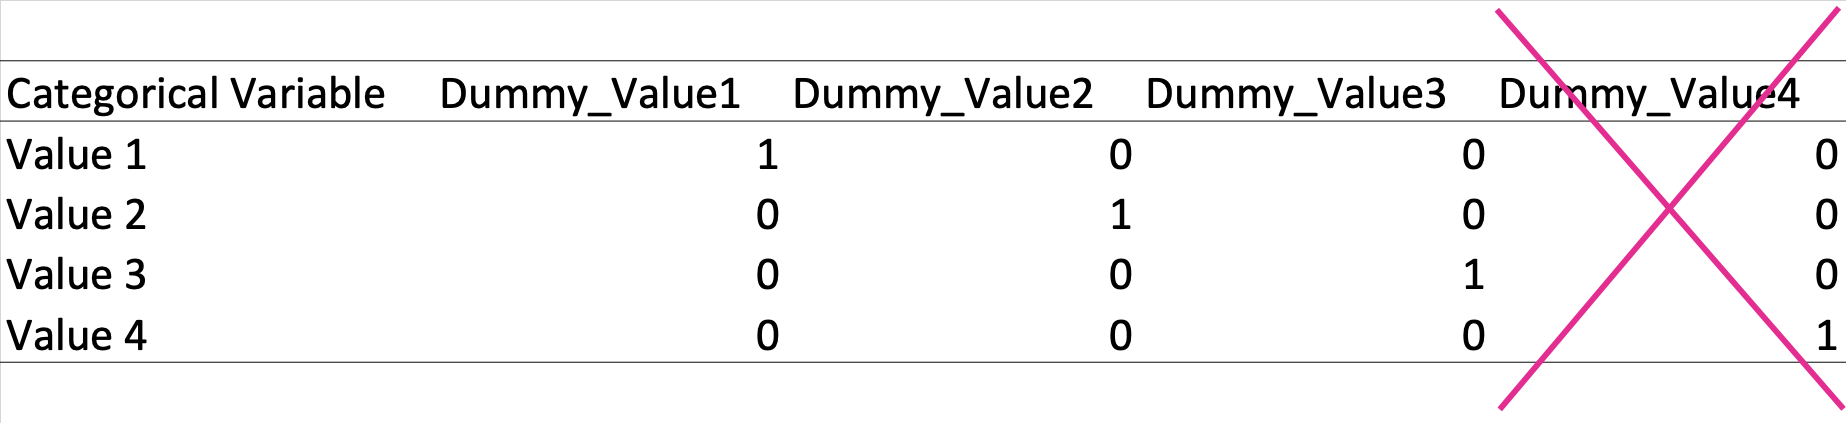
\includegraphics[width=0.625\textwidth]{./MP__encoding.png}
    \caption{Dummy encoding, Omission of one dummy column}
    \label{fig:dp_dumenc}
\end{figure}

\subsection{Missing Data Handling}
A common problem in real data sets is missing information, which needs to be appropriately handled during the modeling process. Popular approaches involve replacing missing values through statistical methods such as mean and median or algorithm-based imputation, such as the k-nearest neighbor Imputer. In the latter case,  the missing value gets imputed with the average value of its k-nearest neighbors, a process detailed in Chapter \ref{sec:kNN}. While another option is to eliminate data entries with missing information, this approach comes with potential drawbacks like information loss and bias. In the case of categorical variables, an alternative method is to treat missing information as a distinct category labeled "Missing", which removes the need for additional adaptations.~\footnote{\cite{Python:2022} p.~207}

\subsection{Erroneous Data Handling}
Erroneous data originating from data entry mistakes or inconsistencies have the potential to introduce noise and bias into the PD modeling process. Expert knowledge is crucial in identifying and rectifying such erroneous data. The best way to reduce incorrect data is control procedures implemented in the data entry systems and a data quality framework, where data validation rules are applied to identify inconsistent or illogical data. These data entries can be treated as missing information for the data preparation process.


\subsection{Outlier Detection and Treatment}
\label{sec:OutlTr}
Extreme values, also called Outliers, can significantly impact the estimated PD model, making expert knowledge crucial in this domain as well. Variables resulting from ratio calculations are especially sensible to outliers, particularly when dealing with division by small numbers. Visual inspection is a simple technique for outlier detection, but this would become impractical with the increasing number of variables. To address this, quantitative approaches become invaluable, utilizing statistical measures such as \ac{IQR}, box plots or Z-scores to identify outliers. A boxplot, also known as a box-and-whisker plot, is a visual representation of the variable's distribution and spread, with the box representing the \ac{IQR} and the whiskers denoting the upper and lower limits. An example is displayed in Figure \ref{fig:dp_iqr_boxpl}. The Z-Score, on the other hand, shows how many standard deviations a data point deviates from the mean of a data set. After the detection, a popular method to treat outliers is winsorization, where all values above or below a certain threshold are capped to the upper and lower limit, thereby minimizing the impact of outliers on the PD model.\footnote{\cite{Python:2022} p.~250}

\begin{figure}[H]
\begin{minipage}{.5\textwidth}
	\begin{align} 
	IQR &= Q_3 - Q_1 \label{eq:dp_iqr_boxpl1}\\
	Upper Limit &= Q_3 + 1.5 \times IQR \label{eq:dp_iqr_boxpl2}\\
	Lower Limit &= Q_1 - 1.5 \times IQR \label{eq:dp_iqr_boxpl3}
	\end{align}
	where:
	\begin{conditions}
	Q_{3}  		& 3.Quartile \\
	Q_{1}  		& 1.Quartile \\
	\end{conditions}
\end{minipage}%
\begin{minipage}{.5\textwidth}
	\centering
	\includegraphics[width=0.9\textwidth]{./MP__boxplot.png}
\end{minipage}
    \caption{Interquartile range and boxplot, Source: \cite{Boxplot:2019}}
    \label{fig:dp_iqr_boxpl}
\end{figure}

\section{Modeling process: Logistic Regression}

\subsection{Variable selection}
During the modeling process, the aim is to estimate a model that shows the best performance within an in-sample and within an out-sample data set. An approach incorporating all available information into the scoring function may indeed yield a high discriminatory power within the trained sample. However, this method usually results in multiple variables exhibiting insignificant coefficients: their p-values fall below the designated confidence level, making it impossible to reject the null hypothesis asserting that the coefficient is, in fact, zero. This outcome not only widens the confidence level but also raises concerns about the accuracy of the coefficient's sign. Therefore, the model's performance on a different data set, especially on more recent data, will most likely deteriorate, leading to unstable predictions. To address this challenge, an extensive analysis of variable performance, considerate selection processes and expert knowledge become crucial.\footnote{\cite{Witzany:2017} p.~44}

\subsubsection{Univariate Analysis}
As a first step, all available variables should be considered for the modeling process. Then, an assessment of the missing rate, detection of outliers and the plausibility of values is conducted. If the variable complies with all data quality requirements, its discriminatory power is then evaluated. This evaluation can be executed using either the univariate Gini coefficient or Information Value. Detailed explanations for both measures are provided in Chapters \ref{sec:gini} and \ref{sec:dataprep}, respectively. The remaining risk factors exhibiting satisfactory discriminatory power form the basis of the long list. 

\subsubsection{Multivariate Analysis}
Maintaining a low level of correlation among model variables is essential to avoid issues related to multicollinearity, which can lead to unstable coefficient estimates in the modeling process. The correlation between two variables can be measured using the Pearson or Spearman correlation coefficient, as detailed in Equations \ref{eq:dp_pears} and \ref{eq:dp_spear}. The Pearson correlation coefficient is more appropriate if a linear relationship is present, while the Spearman correlation coefficient excels in detecting non-linear interactions and can even be used for ordinal variables. The coefficient ranges from -1 (perfect negative correlation) to 1 (perfect positive correlation), with 0 indicating no correlation.\footnote{\cite{FUMS:2020} pp.~129-131}

After computing the coefficients for each variable pair, all values can be arranged into a correlation matrix. An example is visible in Figure \ref{fig:dp_corrmatrix}, which is the heatmap version of Table \ref{tab:re_corr_matrix}. If two variables are highly correlated with a correlation coefficient above a pre-defined threshold, the variable with the lower discriminatory power should be removed from the model list. 

\begin{equation}
\hat{\rho} = \frac{\sum_{i=1}^{n} (x_i - \hat{y}_X)(y_i - \hat{y}_Y)}{\sqrt{\sum_{i=1}^{n} (x_i - \hat{x}_X)^2 \sum_{i=1}^{n} (y_i - \hat{y}_Y)}} \label{eq:dp_pears}
\end{equation}
where:
\begin{conditions}
 x_i, y_i     				& individual observations \\
 \hat{y}_X, \hat{y}_Y    	& sample mean of X and Y  \\
 n    						& number of paired observations
\end{conditions}

\begin{equation}
\rho_s = 1 - \frac{6 \times \sum d_i^2}{n \times (n^2 - 1)} \label{eq:dp_spear}
\end{equation}
where:
\begin{conditions}
 d_{i}  & difference between the ranks of corresponding observations \\
 n    	& number of paired observations
\end{conditions}

\begin{figure}[H]
	\centering
	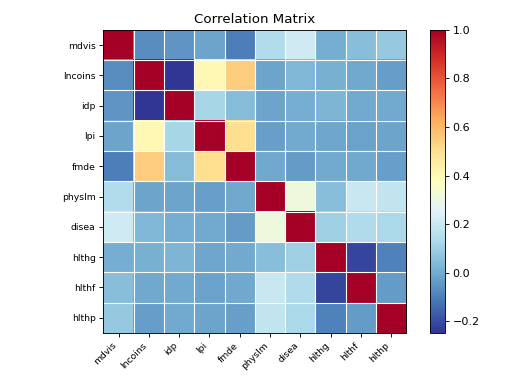
\includegraphics[width=0.625\textwidth]{./MP__corrmatrix.png}
    \caption{Correlation matrix example}
    \label{fig:dp_corrmatrix}
\end{figure}

In the case of categorical variables, the Variance Inflation Factor (VIF, Equation \ref{eq:dp_vif}), which measures the collinearity in the regression analysis, can be utilised. As a final refinement, adjustments based on expert judgment should be applied, allowing disqualified variables into the list or removing variables, even if they meet all criteria. Particular attention should be given to analyzing the relationship between explanatory factors and default rates. If the observed behavior contradicts economic rationale, the variable should be excluded from the model list, also known as the shortlist.\footnote{\cite{Witzany:2017} pp.~45, 53}


\begin{equation}
\text{VIF}_{i} = \frac{1}{1 - R_{i}^2} \label{eq:dp_vif}
\end{equation}
where:
\begin{conditions*}
 R_{i}^2  & coefficient of determination obtained by regressing the i-th regressor on all the other regressors
\end{conditions*}

\subsection{Modeling steps}
Upon identifying the  most promising key factors, there are different approaches to determine the final model variables, specifically, the forward, backward, forward stepwise and backward stepwise selection procedure. The forward approach starts with an empty model and step by step, the variable with the highest discriminatory power is incorporated contingent upon the significance of its coefficient (p-value below a specified threshold). This process continues until no variable satisfies the condition.

Conversely, in the backward selection procedure, the model starts with all variables and those are iteratively removed one by one based on the p-values of their coefficients, until only significant coefficients remain. The forward stepwise procedure combines elements of both with an initially empty model that progressively incorporates variables. However, after each addition, any variable losing significance will be removed. The backward stepwise procedure is the opposite process, starting with all variables and then eliminating those with non-significant coefficients. If, upon exclusion, any variables fulfill the significance condition once more, they are reintroduced into the model.\footnote{\cite{Witzany:2017} p.~45}

To attain a simple model incorporating only the most important risk drivers, the number of variables is limited utilizing the Akaike information criterion (AIC) and Bayesian information criterion (BIC). They are statistical measures used during model selection, which balances the goodness of fit of the model against the complexity by penalizing the inclusion of additional risk factors. At each step of the modeling process, the AIC and BIC are determined and the relative improvement per step is calculated. The model list is cut where a noticeable drop is detected, all subsequent variables are removed from the modeling process and the coefficients are re-estimated, resulting in the final model. 

\section{Modeling Process: Random Forest}

\subsection{Variable selection and Modeling steps}
\label{sec:mp_rf}
During the variable selection process of a normal decision tree, all available features are considered for a split. The evaluation involves assessing  the information gain or Gini impurity improvement for each value of a categorical or indicator variable, as well as for every possible split of a numerical risk factor. A split is executed for the maximum improvement and this process iterates for each resulting subsegment until a stopping condition is fulfilled. Variables that have already been used for a splitting condition maybe considered for a split again. Stopping conditions include achieving homogeneous subgroups, detecting no significant improvement, reaching the minimum leaf size, completing the maximum allowed splits or attaining the maximum depth of the tree.\footnote{\cite{BDT} pp.~2, 4}

As described in Chapter \ref{sec:dectrees}, a Random Forest model is built out of individually trained smaller decision trees and the prediction is a combination of the results of all decision trees, either by calculating the average or using the majority vote. During the training process, only a fraction of all possible features may be selected for the split and optionally, a fraction of the training sample can be used to prevent overfitting. This method is known as Bootstrap Aggregating or Bagging. These steps contribute to a more robust model by avoiding to rely on only a few specific features, which leads to a better generalization. The algorithm demonstrates reduced sensitivity to outliers, as individual decision trees may be affected, but the ensemble tends to mitigate their impact on the overall model. Missing values can still contribute to training the tree by considering other available features or may be randomly removed during the bagging process. A Random Forest model is also relatively robust compared to the logistic regression because, at each split, it selects a random subset of features and this helps in reducing the correlation between a set of features.\footnote{\cite{RanFor:2023}}

\subsection{Hyperparameter Tuning}
Hyperparameters are pre-set configurations of a machine learning algorithm, which are not trained but actually set prior to the training process. Examples are the number of neighbors for the kNN-algorithm, the count of layers in a neural network model or the number of trees in a Random Forest. An optimal configuration of the parameters is crucial because it directly impacts the model's performance to distinguish between the classes as well as influences overfitting. Adjusting these parameters is an individualized task, dependent on the unique characteristics of each problem, encompassing factors like the number and type of features, data size and data quality. With an increasing number of hyperparameters, the combination possibilities become extensive, making the search for the optimal configuration time-consuming. Therefore, the objective is to quickly identify a good configuration and subsequently search for potentially better settings.

Initially, a wide range of hyperparameter values is defined and the model's performance is assessed through randomly chosen combinations for a predefined number of iterations. The best combination is then utilized for the subsequent grid search. In this phase, a more constrained range for each hyperparameter, centered around the optimized configuration, is defined. All possible combinations within this scope are evaluated and the superior outcome from both approaches forms the final model configuration.\footnote{\cite{Python:2022} p.~465} \footnote{\cite{RanFor:2023}}

\subsection{k-Fold Cross Validation}
To further avoid overfitting, a cross-validation can be incorporated during the hyperparameter tuning process. The data set is randomly split into equally sized k subsamples, also called folds. The model with the tested hyperparameters is then trained on k-1 subsets and their performance is evaluated on the unused data set. This step is repeated k-times, with a different fold used for evaluation each time. The overall performance is calculated by averaging the metrics across all subsamples. This comprehensive process will be performed for each configuration setting during the random or grid search, contributing to a more robust model. An illustrative sketch is provided in Figure \ref{fig:re_wholesample}.\footnote{\cite{Python:2022} p.~470}

\begin{figure}[H]
	\centering
	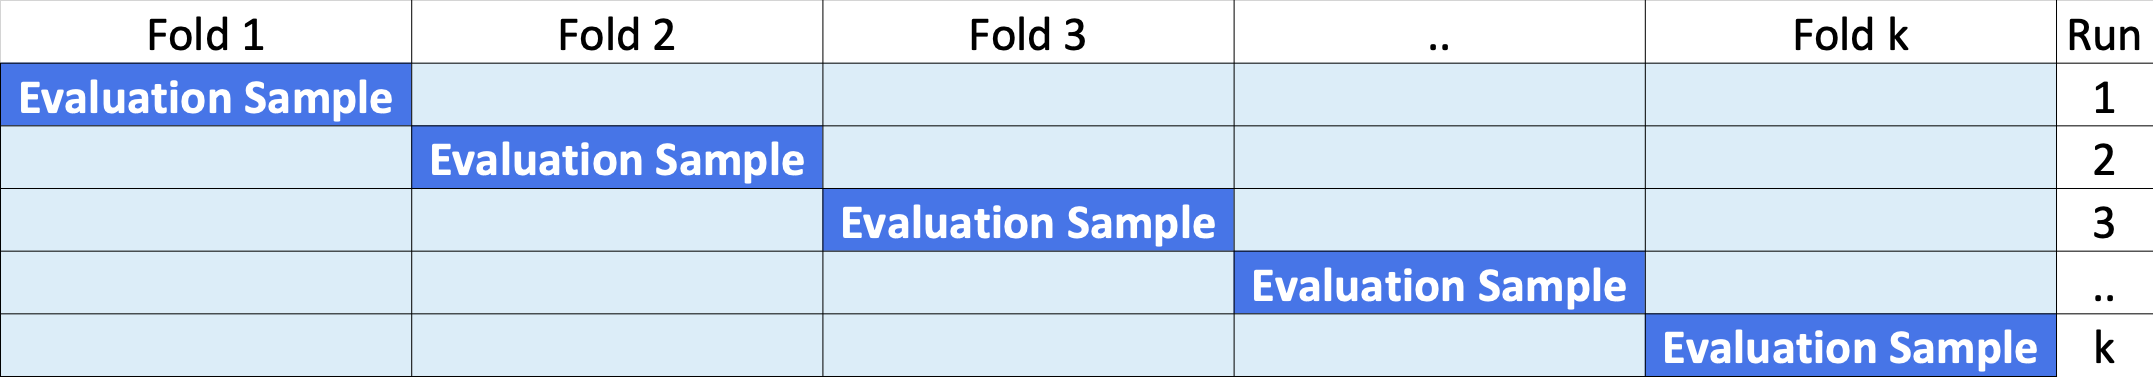
\includegraphics[width=0.65\textwidth]{./MP__kFold.png}
    \caption{k-Fold Cross Validation}
    \label{fig:re_wholesample}
\end{figure}

\chapter{Validation}

\section{Out-of-Sample and Out-of-Time Validation}
Out-of-sample validation involves evaluating the model's performance on a data set that was not used during its development. Taking it a step further, out-of-time validation introduces new data, covering a more recent time period. The objective is to assess the model's ability to make accurate predictions on unseen data. Because the model is estimated on the training sample, it is not uncommon for it to exhibit better performance on in-sample datasets compared to other samples. However, if the performance metrics differs significantly, it could signal overfitting. The full dataset is usually split into a 70\% training and 30\% testing sample, also referred to as validation sample. Different ratios, such as 60/40 or 80/20, are also popular choices and mainly depends on the dataset size and the number of default events. During the splitting process it is important to keep the number of default events even in both samples to prevent scenarios, where one class is disproportionally larger than the other. This method called stratification reduces the probability of a biased model training and evaluation process. \cite[p.~27]{Witzany:2017}

\section{Model Performance Evaluation}

\subsection{Confusion matrix}
The confusion matrix, illustrated in Figure \ref{fig:vl_confmatr}, is a table comprising four elements, which shows the count of observations correctly (True Positive, True Negative) and incorrectly (False Positive, False Negative) identified cases. A False Positive, denoting a customer predicted to default but survived, is also called Type I Error. A False Negative, where a borrower is expected to survive but defaulted, is also known as Type II error. In practice, a Type II error holds greater severity, as the repercussions of a defaulted exposure outweigh the missed opportunity income from rejecting a non-defaulted application. \cite[p.~29.30]{Witzany:2017}

\begin{figure}[H]
	\centering
	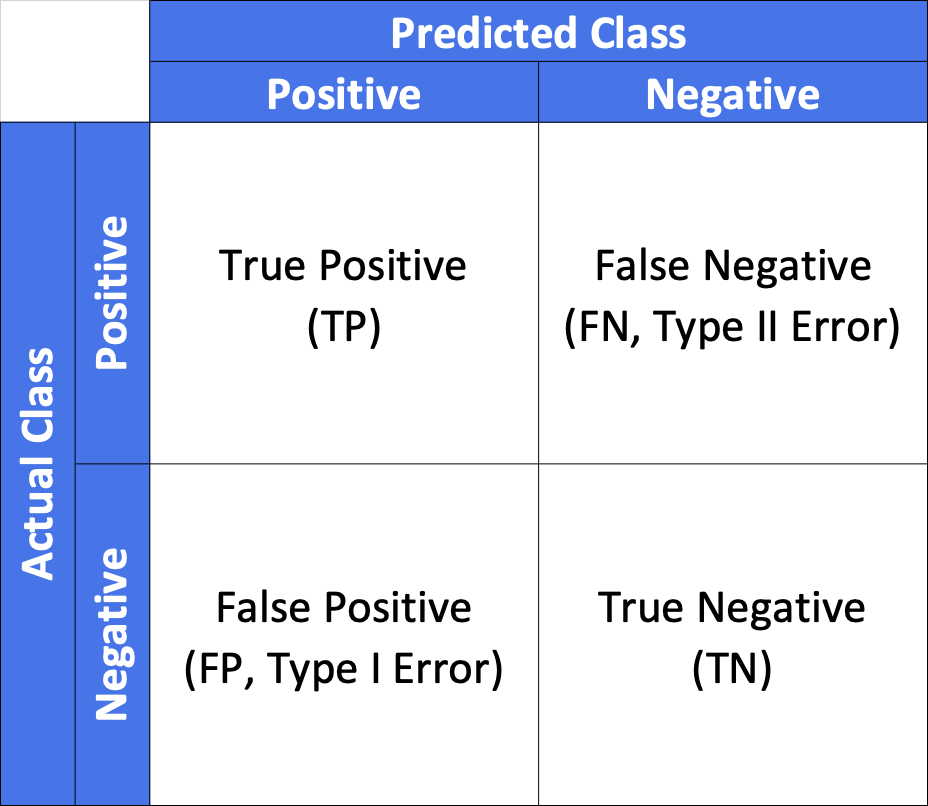
\includegraphics[width=0.45\textwidth]{./VL__confmatrix.png}
    \caption{Confusionmatrix}
    \label{fig:vl_confmatr}
\end{figure}

Using the elements of the confusion matrix, the measures Accuracy, Precision, Recall, F1-Score and others can be calculated, as illustrated in Equations \ref{eq:vl_sens} to \ref{eq:vl_f1}. However, measures like Accuracy and Precision are not recommended for unbalanced data, because they can provide misleading insights about the model's performance. In instances of unbalanced data, a model might attain a high accuracy by simply predicting only the majority class. This high accuracy overshadows the model's ability to correctly identify observations of the minority class. In such scenarios, Recall and F1-score provide a more accurate evaluation of the model's performance. For the transformation from PD to a predicted default flag a threshold has to be selected. To determine an ideal cut-off, the F1-Score can be utilized, where the value is set where the F1-score attains its maximum. \cite{AUC:2023}

\begin{flalign} 
\text{Sensitivity} &= \frac{\text{True Positives}}{\text{True Positives} + \text{False Negative}} \\[10pt] \label{eq:vl_sens}
\text{Specificity} &= \frac{\text{True Negative}}{\text{True Negative} + \text{False Positives}} \\[10pt]
\text{Precision} &= \frac{\text{True Positives}}{\text{True Positives} + \text{False Positives}} \\[10pt]
\text{Negative Predictive Value} &= \frac{\text{True Negative}}{\text{True Negative} + \text{False Negative}} \\[10pt]
\text{Accuracy} &= \frac{\text{True Positives} + \text{True Negatives}}{\text{Total Population}} \\[10pt]
\text{Recall} &= \frac{\text{True Positives}}{\text{True Positives} + \text{False Negatives}} \\[10pt]
\text{F1-Score} &= 2 \times \frac{\text{Precision} \times \text{Recall}}{\text{Precision} + \text{Recall}} \label{eq:vl_f1}
\end{flalign}

\subsection{Receiver Operating Characteristic Curve}

The Receiver Operating Characteristic Curve (ROC Curve, see Figure \ref{fig:vl_roccurve}) is the resulting curve after plotting the proportion of False Positive along the x-axis and proportion of True Positive along the y-axis. A diagonal line between (0,0) and (0,1) represents the random model, while the perfect model's curve would be a step function that starts at (0,0) straight up and moves horizontally to (1,1). The Area Under the ROC-Curve (AUC-ROC Curve) is, as the name suggests, the area below the ROC-curve and the formula for calculating the AUC is Equation \ref{eq:vl_auc}. \cite{AUC:2023}

\begin{equation}
AUC = A + \frac{1}{2} \label{eq:vl_auc}
\end{equation}

\subsection{GINI coefficient}
\label{sec:gini}
The Gini coefficient and AUC are connected via the given Equation \ref{eq:vl_gini} and a visual presentation is visible in Figure \ref{fig:vl_roccurve}, the areas are designated as A and B. Therefore, they relate the same information but are differently scaled and the Gini coefficient shows an improved interpretability. While the AUC has a range between 0.5 (random model) to 1 (perfect model), the Gini coefficient takes on values between 0 (no discriminatory power) and 1 (perfect discriminatory power). In general, the AUC can also take on a value below 0.5, but that would indicate, that the model's predictions are less accurate than the random model, indicating an issue in the model's ability to differentiate between the classes. \cite{AUC:2023}

\begin{equation}
GINI = \frac{A}{A + B} = \frac{A}{\frac{1}{2}} = (2 * A + 1) - 1 = 2 * \text{AUC} - 1 \label{eq:vl_gini}
\end{equation}

\begin{figure}[H]
	\centering
	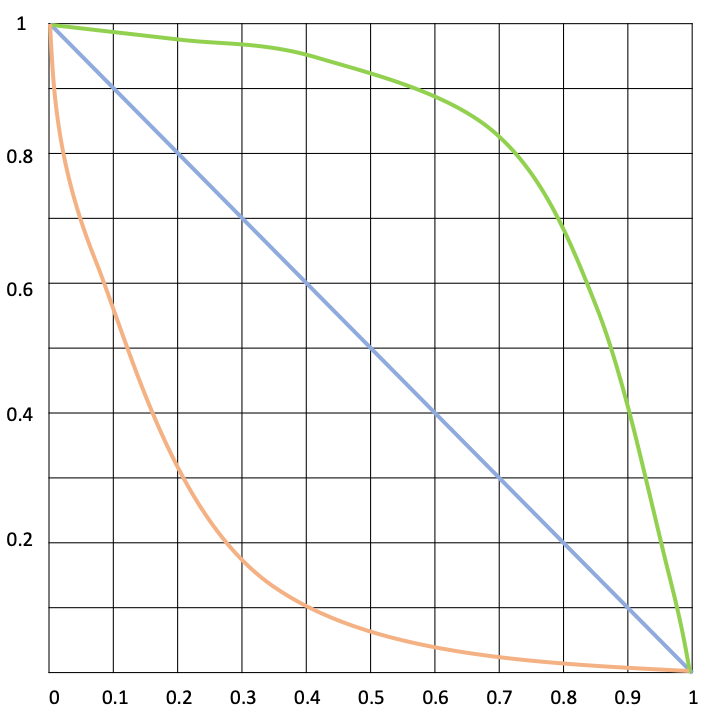
\includegraphics[width=0.625\textwidth]{./VL__ROC_curve.png}
    \caption{AUC-ROC curve}
    \label{fig:vl_roccurve}
\end{figure}

\section{Stability Test}
Stability testing is performed to assess the robustness and consistency of a PD model over time. It examines whether the model's performance remains stable and reliable when applied to data collected at different time periods. Stability testing helps identifying potential model deterioration or drift over time, which may be caused by changes in the underlying credit conditions or data characteristics. If significant discrepancies are detected, model recalibration or updates may be necessary to maintain its accuracy and relevance.

\chapter{Interpretability}
\label{sec:interpret}

\section{Importance of Interpretability}
Interpretability refers to the capability to explain and understand how a model arrives at its predictions or decisions. Regression models and decision trees are simple to understand and thus very popular in the banking industry. In contrary, more advanced machine learning models show a black box nature; their model logic and output are difficult to explain. Machine learning models' complex structure have advantages and disadvantages. While they can detect non-linear relationships and correlations, and may show improved accuracy or efficiency, they are also prone to overfitting and lack explainability. Their black box nature stems from the model's numerous transformation of input variables, as well as their optimization process. \cite[p.~56]{Roberts2022}

\subsection{Regulatory and Legal Requirements}
\label{sec:ref_leg}

Interpretability enables compliance with regulations and consumer protection laws such as the Capital Requirements Regulation (CRR) and General Data Protection Regulation (GDPR). Data protection principles such as purpose limitation, data minimisation and limitation on automated decisions are evident obstacles for complex AI models. In the CRR (Capital Requirements Regulation, Article 144(1)(a)), a requirement of the PD model development is stated as:

\begin{quote}

(a) the institution's rating systems provide for a meaningful assessment of obligor and transaction characteristics, a meaningful differentiation of risk and accurate and consistent quantitative estimates of risk;

\end{quote}

Regulations mandate that both model developers and users provide explanations for credit-related decisions to their customers. Modelers, along with internal and external auditors, are obligated to validate not only the model's structure but also its results, ensuring whether the model aligns with domain knowledge and expectations. Interpretability helps identifying potential biases, data issues or model limitations. Additionally, a unexplainable model used in production increases operational risk, as it becomes challenging to assess potential consequences, such as bias or fairness, and verify the accuracy of results or detect system errors. To circumvent the constraints imposed by regulatory requirements and consumer protection laws, machine learning models may find application in areas where the model's structure and output are not of utmost priority, such as in the collection process or fraud detection. \cite[pp.~57, 58]{Roberts2022} \cite[p.~89]{Witzany:2017}

\subsection{Data Management}
Before the development or deployment of machine learning models, a sound data management process has to be established. The training data must be unbiased and accurately reflect the population the model will be deployed on, meaning that individual groups should not be over- or underrepresented. Failure to correct and validate the data utilized during the training phase or in production can yield unexpected outcomes or result in a biased model. Machine learning algorithms have the potential to amplify errors, as popular saying goes, "Garbage In - Garbage Out." \cite[p.~61]{Roberts2022}

\section{Methods for Interpretability Analysis}
Techniques to asses the interpretability of advanced models are also called model-agnostic explainability methods. They are algorithm independent, usually applied after model development and assess on global or local level, which means on dataset or data observation level. Depending on the objective, the techniques can be allocated into five categories: feature importance, input variable impact, specific prediction analysis, output analysis and robustness check. \cite[p.~62]{Roberts2022}

\subsection{Feature Importance}
Feature importance measures the contribution of each variable in a predictive model to the overall model performance. If the performance drops significantly when changing the value of a variable while keeping other risk factors constant, implies the importance of that particular feature. Relative feature importance compares the importance of features relative to each other, which helps in prioritizing features based on their influence on the model's predictions. To facilitate a meaningful comparison, the ranges of each variable need to be normalized to the same scale, enabling a direct assessment of their impact. \cite[p.~63]{Roberts2022}

\begin{figure}[H]
	\centering
	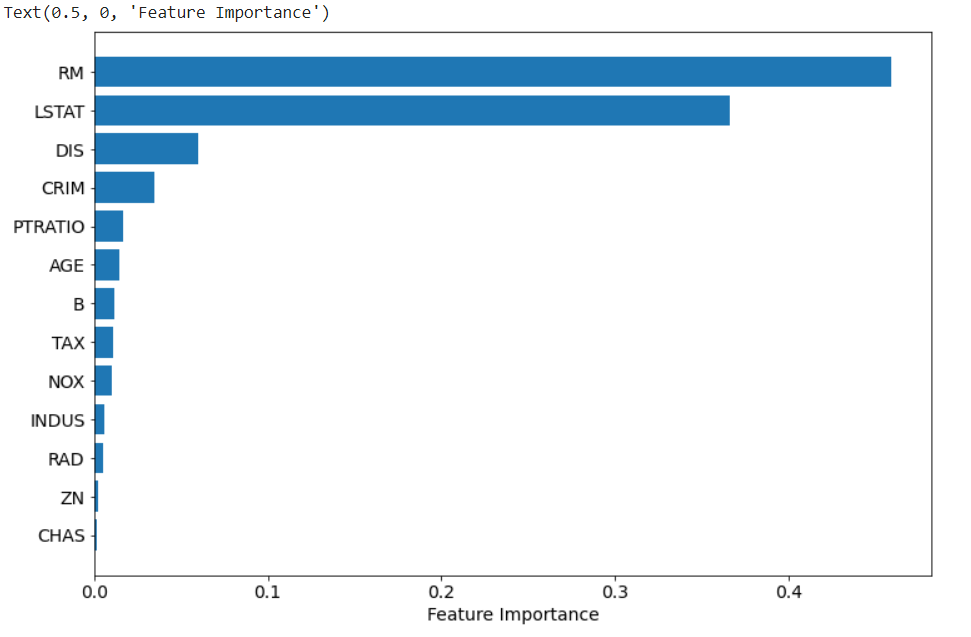
\includegraphics[width=0.625\textwidth]{./IN__featureimp.png}
    \caption{Feature Importance}
    \label{fig:in_featureimp}
\end{figure}

\subsection{Input Variable Impact}
Exploring the impact of individual variables is carried out through techniques like Partial Dependence Plots (PDP) and Individual Conditional Expectation (ICE), illustrated in Figure \ref{fig:in_pdp}. PDP visualises the relationship between a specific feature and the model's predictions while holding other variables constant. They provide insights into the direction and magnitude of the feature's effect on default probability. ICE is an extension of PDP, where it illustrates how predictions change for an individual data point as a specific feature varies. \cite[p.~63]{Roberts2022}

\begin{figure}[H]
\begin{minipage}{.5\textwidth}
	\centering
	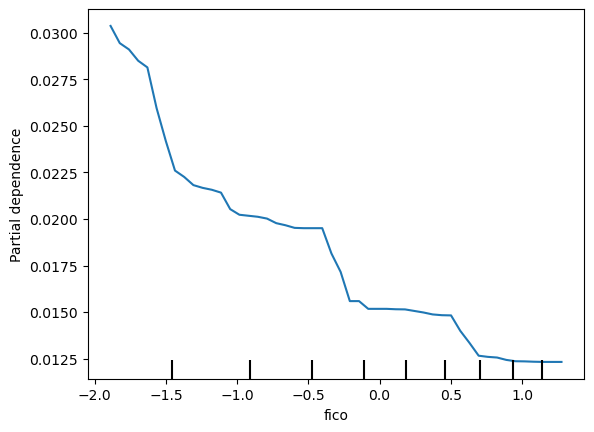
\includegraphics[width=0.9\textwidth]{./plot/ML/PDP_fico.png}
    \caption{Partial Dependence Plots}
    \label{fig:in_pdp}
\end{minipage}%
\begin{minipage}{.5\textwidth}
	\centering
	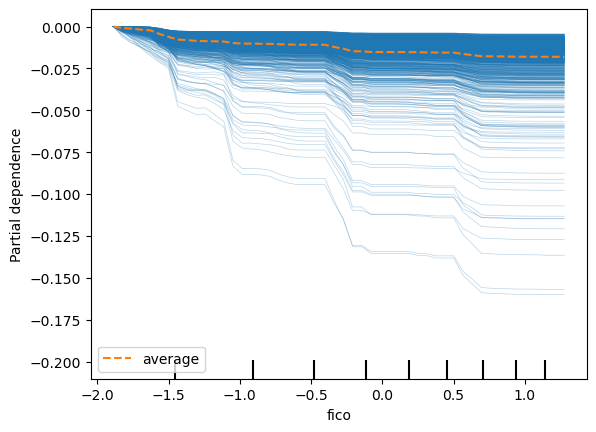
\includegraphics[width=0.9\textwidth]{./plot/ML/ICE_fico.png}
    \caption{Individual Conditional Expectation}
    \label{fig:in_ice}
\end{minipage}
\end{figure}

\subsection{Individual Prediction Analysis}
For the interpretation of specific predictions, tools such as Local Interpretable Model-Agnostic Explanations (LIME) and Local rule-based explanations can be utilized. In the LIME process, a local interpretable surrogate model is estimated. A small sample with similar variable values is selected and used to estimate a sparse linear regression model while using the predictions of the machine learning models as target. Similarly, the Local rule-based explanations method builds a set of decision rules to act as a surrogate model in the interpretation process. \cite[p.~65-67]{Roberts2022}

\subsection{Output Analysis and Robustness Check}
During Counterfactual analysis, the feature values are slowly changed to assess, which total changes are necessary to receive a specific prediction. Adversial testing is performed to analyze, how the machine learning model reacts to adversial attacks, which are input data deliberately designed with the aim of causing misclassification or incorrect output. Internal layers of Deep Neural Networks can be computed to detect adversial data to respond accordingly. Alternatively, adversial data can be incorporated in the development sample to include them during the training phase. In a sensitivity test, data with value ranges not captured by the training sample are used to analyze the model predictions and their performance beyond its training scope. \cite[p.~65-67]{Roberts2022}


\chapter{Used Data and Results}
\label{ch:RE}
\section{Freddie Mac's Single Family Loan-Level Data set}

Freddie Mac, officially known as the Federal Home Loan Mortgage Corporation, is a government-sponsored enterprise (GSE) in the United States and plays a crucial role in the secondary mortgage market. In the primary market, individual customers secure mortgage loans from retail banks. Within the secondary mortgage market, the lender has the option to sell these mortgages to entities like government-sponsored enterprises, e.g., Freddie Mac. This practice provides liquidity to the primary market, subsequently making additional loans available to other customers. GSEs aggregate multiple mortgages into mortgage-backed securities (MBS), which are then sold to various investors, such as insurance companies and hedge funds.\footnote{\cite{FreddieMac:2023}}\footnote{\cite{SecMortMark:2023}}

The Single Family Loan-Level Data set encompasses a broad range of variables and some of the essential features of this data set include:

\begin{enumerate}
\item Customer Information: This category includes borrower details such as Credit Score provided by FICO, first-time homebuyer status, occupancy status and number of borrowers.
\item Financial Attributes: The data set provides important financial indicators such as the (combined) loan-to-value ratio (CLTV, LTV) and debt-to-income ratio (DTI).
\item Loan and Property Details: It also includes information about the properties associated with the loans, such as mortgage insurance percentage, number of units, original unpaid balance, original Loan Term, property type and loan purpose.
\item Loan Performance: This section captures essential data related to historical loan performance. It includes details on delinquency status, zero balance reason codes, modification information and the current deferred unpaid balance.
\item Expenses and Loss Information: Included in the performance data are financial details such as mortgage insurance recoveries, net sale proceeds, legal costs and actual loss, among others.
\end{enumerate}

\subsection{Data Quality, Limitations and Usage}

Over the years, Freddie Mac has accumulated vast amounts of mortgage loan data. At the direction of the Federal Housing Finance Agency (FHFA), this data has been made publicly available to enhance transparency and assist investors in analyzing credit performance. Freddie Mac's Single Family Loan-Level Data set is publicly available on their website, where users are required to register and agree to the data set's terms of use before accessing the data.\footnote{\cite{FreddieMacData:2023}}

While the Single Family Loan-Level Data set offers a wealth of information, it is essential to consider its quality and limitations. Freddie Mac explicitly states  that they do not guarantee a complete or error-free data set and that it may contain potential biases. The data set represents mortgages acquired by Freddie Mac, which may not be fully representative of the entire mortgage market. Furthermore, the data set is subject to data protection regulations leading to the anonymization or removal of personally identifiable information. The data set is updated quarterly and thus contains corrections or updates that may impact the analysis.\footnote{\cite{FreddieMacUG:2023}}


\section{Data set}

The Freddie Mac Data set consists of the origination and monthly performance data files. The former contains information about the borrower and the mortgage loan collected at the start of the contract. The latter includes monthly snapshots of the mortgage loan's payment, status and loss history. The data preparation and modeling process focuses on the origination data, as the objective is creating an application scoring model. The monthly performance data will be used to approximate a default flag, described in Chapter \ref{sec:aprox_def}. The provided data files cover all months since January 1999 and undergo continuous updates every quarter. On average, each month contains about 157.000 mortgage loans, with the highest number of mortgage loans opened in September 2003 with 577.000 accounts. Table \ref{tab:re_descr} shows the full list of relevant variables, their description and abbreviation:

\newpage

\begin{longtable}{ Lp{8cm}R }\toprule
\textbf{Variable Name}                             & \textbf{Description}                                                                                                                                                                                                                                                                          & \textbf{Abbr.}       \\\midrule
Credit Score                              & A score from an external source (FICO), indicating the borrower's creditworthiness. The higher the score, the lower the probability of default. Value ranges between 300 and 850 or a value of 9999 will be set.                                                                     & Credit Score       \\\hline
First Time Homebuyer Flag                 & Variable is set to 'Y' if borrower purchased the mortgaged property to use as a primary residence and had no ownership in a different property in preceeding three years before purchase.                                                                                            & Homebuyer Flag     \\\hline
Mortgage Insurance Percentage (MI \%)     & Percentage of loss coverage on the loan, that a mortgage insurer covers after a default. Value ranges between 1\% and 55\% or a value of 999 will be set.                                                                                                                            & MI Perc            \\\hline
Number of Units                           & Number of units in property. Value ranges between 1 and 4 or a value of 99 will be set.                                                                                                                                                                                              & No Units           \\\hline
Occupancy Status                          & Contains values "Primary Residence", "Investment Property", "Second Home", "Not Available"                                                                                                                                                                                           & Occupancy          \\\hline
Original Combined Loan-to-Value (CLTV)    & Ratio: (Original mortgage loan amount + Secondary mortgage loan amount if available) divided by the mortgaged property’s appraised value. Value ranges between 1\% and 998\% or a value of 999 will be set. If the CLTV is lower than CTV, then the value was set to 999.            & CLTV               \\\hline
Original Debt-to-Income (DTI) Ratio       & Ratio: (Monthly debt payments + housing expenses) divided by (monthly income). Value ranges between 0\% and 65\% or a value of 999 will be set.                                                                                                                                      & DTI                \\\hline
Original UPB                              & Unpaid principal balance rounded to the nearest 1.000                                                                                                                                                                                                                                & UPB                \\\hline
Original Loan-to-Value (LTV)              & Ratio: Original mortgage loan amount divided by lesser of the mortgaged property’s appraised value. Value ranges between 1\% and 998\% or a value of 999 will be set.                                                                                                                & LTV                \\\hline
Channel                                   & Contains values "Retail", "Broker", "Correspondent", "TPO Not Specified",  "Not Available"                                                                                                                                                                                           & Channel            \\\hline
Prepayment Penalty Mortgage (PPM) Flag    & Variable is set to 'Y' if borrower is or was obligated to pay a penalty in the event of certain repayments of principal.                                                                                                                                                             & PPM Flag           \\\hline
Amortization Type (Formerly Product Type) & Contains values "Fixed Rate Mortgage",  "Adjustable Rate Mortgage"                                                                                                                                                                                                                   & Amort Type         \\\hline
Property State                            & Two letter statecode of property                                                                                                                                                                                                                                                     & State              \\\hline
Property Type                             & Contains values "Condo", "PUD", "Manufactured Housing", "Single-Family",  "Co-op", "Not Available"                                                                                                                                                                                   & Prop Type          \\\hline
Loan Purpose                              & Contains values "Purchase", "Refinance - Cash Out", "Refinance - No Cash Out", "Not Available"                                                                                                                                                                                       & Loan Purpose       \\\hline
Original Loan Term                        & Number of scheduled monthly payments.                                                                                                                                                                                                                                                & Loan Term          \\\hline
Number of Borrowers                       & Number of borrowers obligated to repay the mortgage. Value ranges between 1 and 10 or a value of 99 will be set.                                                                                                                                                                     & No Borrowers       \\\hline
Super Conforming Flag                     & Variable is set to 'Y' if mortgage loan exceed conforming loan limits.                                                                                                                                                                                                               & Sup Conf Flag      \\\hline
Program Indicator                         & Contains values "Home Possible", "HFA Advantage", "Refi Possible", "Not Available", "Not Applicable"                                                                                                                                                                                 & Prog Flag          \\\hline
HARP Indicator                            & Variable is set to 'Y' if loan is part of Freddie Mac’s Relief Refinance Program                                                                                                                                                                                                     & HARP Flag          \\\hline
Property Valuation Method                 & Contains values "Relief Refinance Loan", "Non-Relief Refinance loan"                                                                                                                                                                                                                 & Prop Val Method    \\\hline
Interest Only (I/O) Indicator             & Variable is set to 'Y' if loan only requires interest payments at the beginning of contract.                                                                                                                                                                                         & Int Only Flag      \\\hline
Current Loan Delinquency Status           & Number of days the borrower is delinquent and calculated under the Mortgage Bankers Association (MBA) method                                                                                                                                                                         & Delinquency Status \\\hline
Zero Balance Code                         & Reason, why the loan's balance was reduced to zero; Contains values "Prepaid or Matured (Voluntary Payoff)", "Third Party Sale", "Short Sale or Charge Off", "Repurchase prior to Property Disposition", "REO Disposition", "Whole Loan sales", "Reperforming sales securitizaitons" & Zero Balance Code 
%\end{tabular}
%\end{table}
\\\bottomrule

\caption{Description of variables}
\label{tab:re_descr}
\end{longtable}

\subsection{Approximation of default flag}
\label{sec:aprox_def}

Since the data set does not directly contain default information, an approximation for the indicator needs to be created. This information is derived from the performance data of the mortgage loan. As a first step, the number of months between the date of the first payment and the date of being in delinquency continuously for 30/60/90/120/180 days was calculated. To imitate the definition of default described in the CRR 178(1a), see Chapter \ref{sec:dr_pd}, as closely as possible, the 90 \ac{DPD} delinquency information was selected for further analysis. Due to data irregularities, where the 120 \ac{DPD} or 180 \ac{DPD} field is filled in, but the 90 \ac{DPD} is missing, the minimum of all three variables was used for the next steps. Additionally, to fulfill the definition of default stated in the CRR 178(1b), the variable \emph{Zero Balance Code} was incorporated. It contains the reason why the loan balance was reduced to zero, displayed in Table \ref{tab:re_ZB_Descr}. Therefore, Zero Balance Codes 02, 03, 09 and 15 indicate a negative financial health and were considered in the default approximation.


\begin{table}[H]
\centering
\begin{tabular}{ l l }\toprule
\textbf{Zero Balance Code} & \textbf{Description}            \\\midrule
01                & Prepaid or Matured (Voluntary Payoff)    \\
02                & Third Party Sale                         \\
03                & Short Sale or Charge Off                 \\
96                & Repurchase prior to Property Disposition \\
09                & REO Disposition                          \\
15                & Whole Loan sales                         \\
16                & Reperforming sales securitizaitons \\\bottomrule
\end{tabular}%
\caption{Description of Zero Balance Code}
\label{tab:re_ZB_Descr}
\end{table}

In the modeling process, a 12-month time span was chosen. Following the identification of default events, the default flag was set based on the following conditions:

\begin{itemize}
  \item Customer was in delinquency for at least 90 days continuously during the first 12 months in the books.
  \item Loan balance showed a negative behavior in the \emph{Zero Balance Code} during the first 12 months in the books.
\end{itemize}

\section{Sample Creation}

\subsection{Data Exclusions}
The first two months of the whole data set showed an unusually low number of observations and default events, leading to their exclusion. Given the 12-month observation period for the default flag, the final 12 months of the data set were also omitted. Additionally, accounts prepaid before the 12-month observation period ended were removed. Lastly, mortgage loans without monthly performance data were also deleted because it was impossible to approximate a default flag. The breakdown of exclusions based on each reason is detailed in Table \ref{tab:re_nr_excl}.

\begin{table}[H]
\centering
\begin{tabular}{ l r }\toprule          										
\textbf{Reason}                                       	& \textbf{Number of data entries} 	\\\midrule
Remove first 2 months due to unusual low number 		& 5047                   			\\
Less than 12 months (Last Year)                 		& 2127828                			\\
Less than 12 months and prepaid                 		& 4452984                			\\
Missing Monthly Performance data                		& 1484  				 			\\\bottomrule
\end{tabular}%
\caption{Number of exclusions}
\label{tab:re_nr_excl}
\end{table}

\subsection{Training, Test and Validation Sample}
Figure \ref{fig:re_wholesample} shows the monthly default rate for the whole sample before and after data exclusions and Figure \ref{fig:re_devsample} is a separate display of the development and out-of-time sample, also referred to as validation sample. The vertical line in Figure \ref{fig:re_devsample} separates the development sample, which is split into training and test data set and validation sample. If the number of default events had not been sufficient, an increase in the observation window might have been a solution. Both figures show a satisfying number of monthly defaults with an average default rate of 1,52\% in the development sample. A plausible development of the default rate is visible; it follows the expected increase of defaults during the Dot-Com crisis in the late 1990s, the financial crisis in 2007/2008 and the COVID-19 crisis in 2020/2021. 

The development sample encompasses data from January 2018 to December 2020, offering a timeframe that covers different economic conditions, including the period before and during the COVID-19 crisis. This selection not only captures diverse economic scenarios but also limits the number of observations due to the limitation of computational power. The out-of-time sample is constructed using data points from January to December 2021. 

The data preparation and univariate analysis were performed on the whole development data set, then split into 70\% training and 30\% test samples. The split was stratified on the default flag and the year to ensure a balanced data set for the multivariate analysis and the modeling process of both modeling approaches. Table \ref{tab:re_devoofsample} shows the sample sizes and default rates. Complete lists of the number of accounts and defaults per month for the whole sample before and after exclusion are given in Appendix \ref{sec:DR_whole}.

\begin{table}[H]
\centering
\begin{tabular}{lrrr} \toprule       
\textbf{Sample} & \textbf{\# Accounts} & \textbf{\# Def} & \textbf{\% Def Rate} \\\midrule
Whole Data set   & 39.404.062           & 208.008         & 0,53\%               \\
Training        & 3.789.579            & 57.510          & 1,52\%               \\
Test            & 1.624.101            & 24.645          & 1,52\%               \\
Out Of Time     & 4.121.718            & 16.848          & 0,41\%               \\\bottomrule
\end{tabular}
\caption{Development and Validation sample}
\label{tab:re_devoofsample}
\end{table}

\begin{figure}[H]
	\centering
	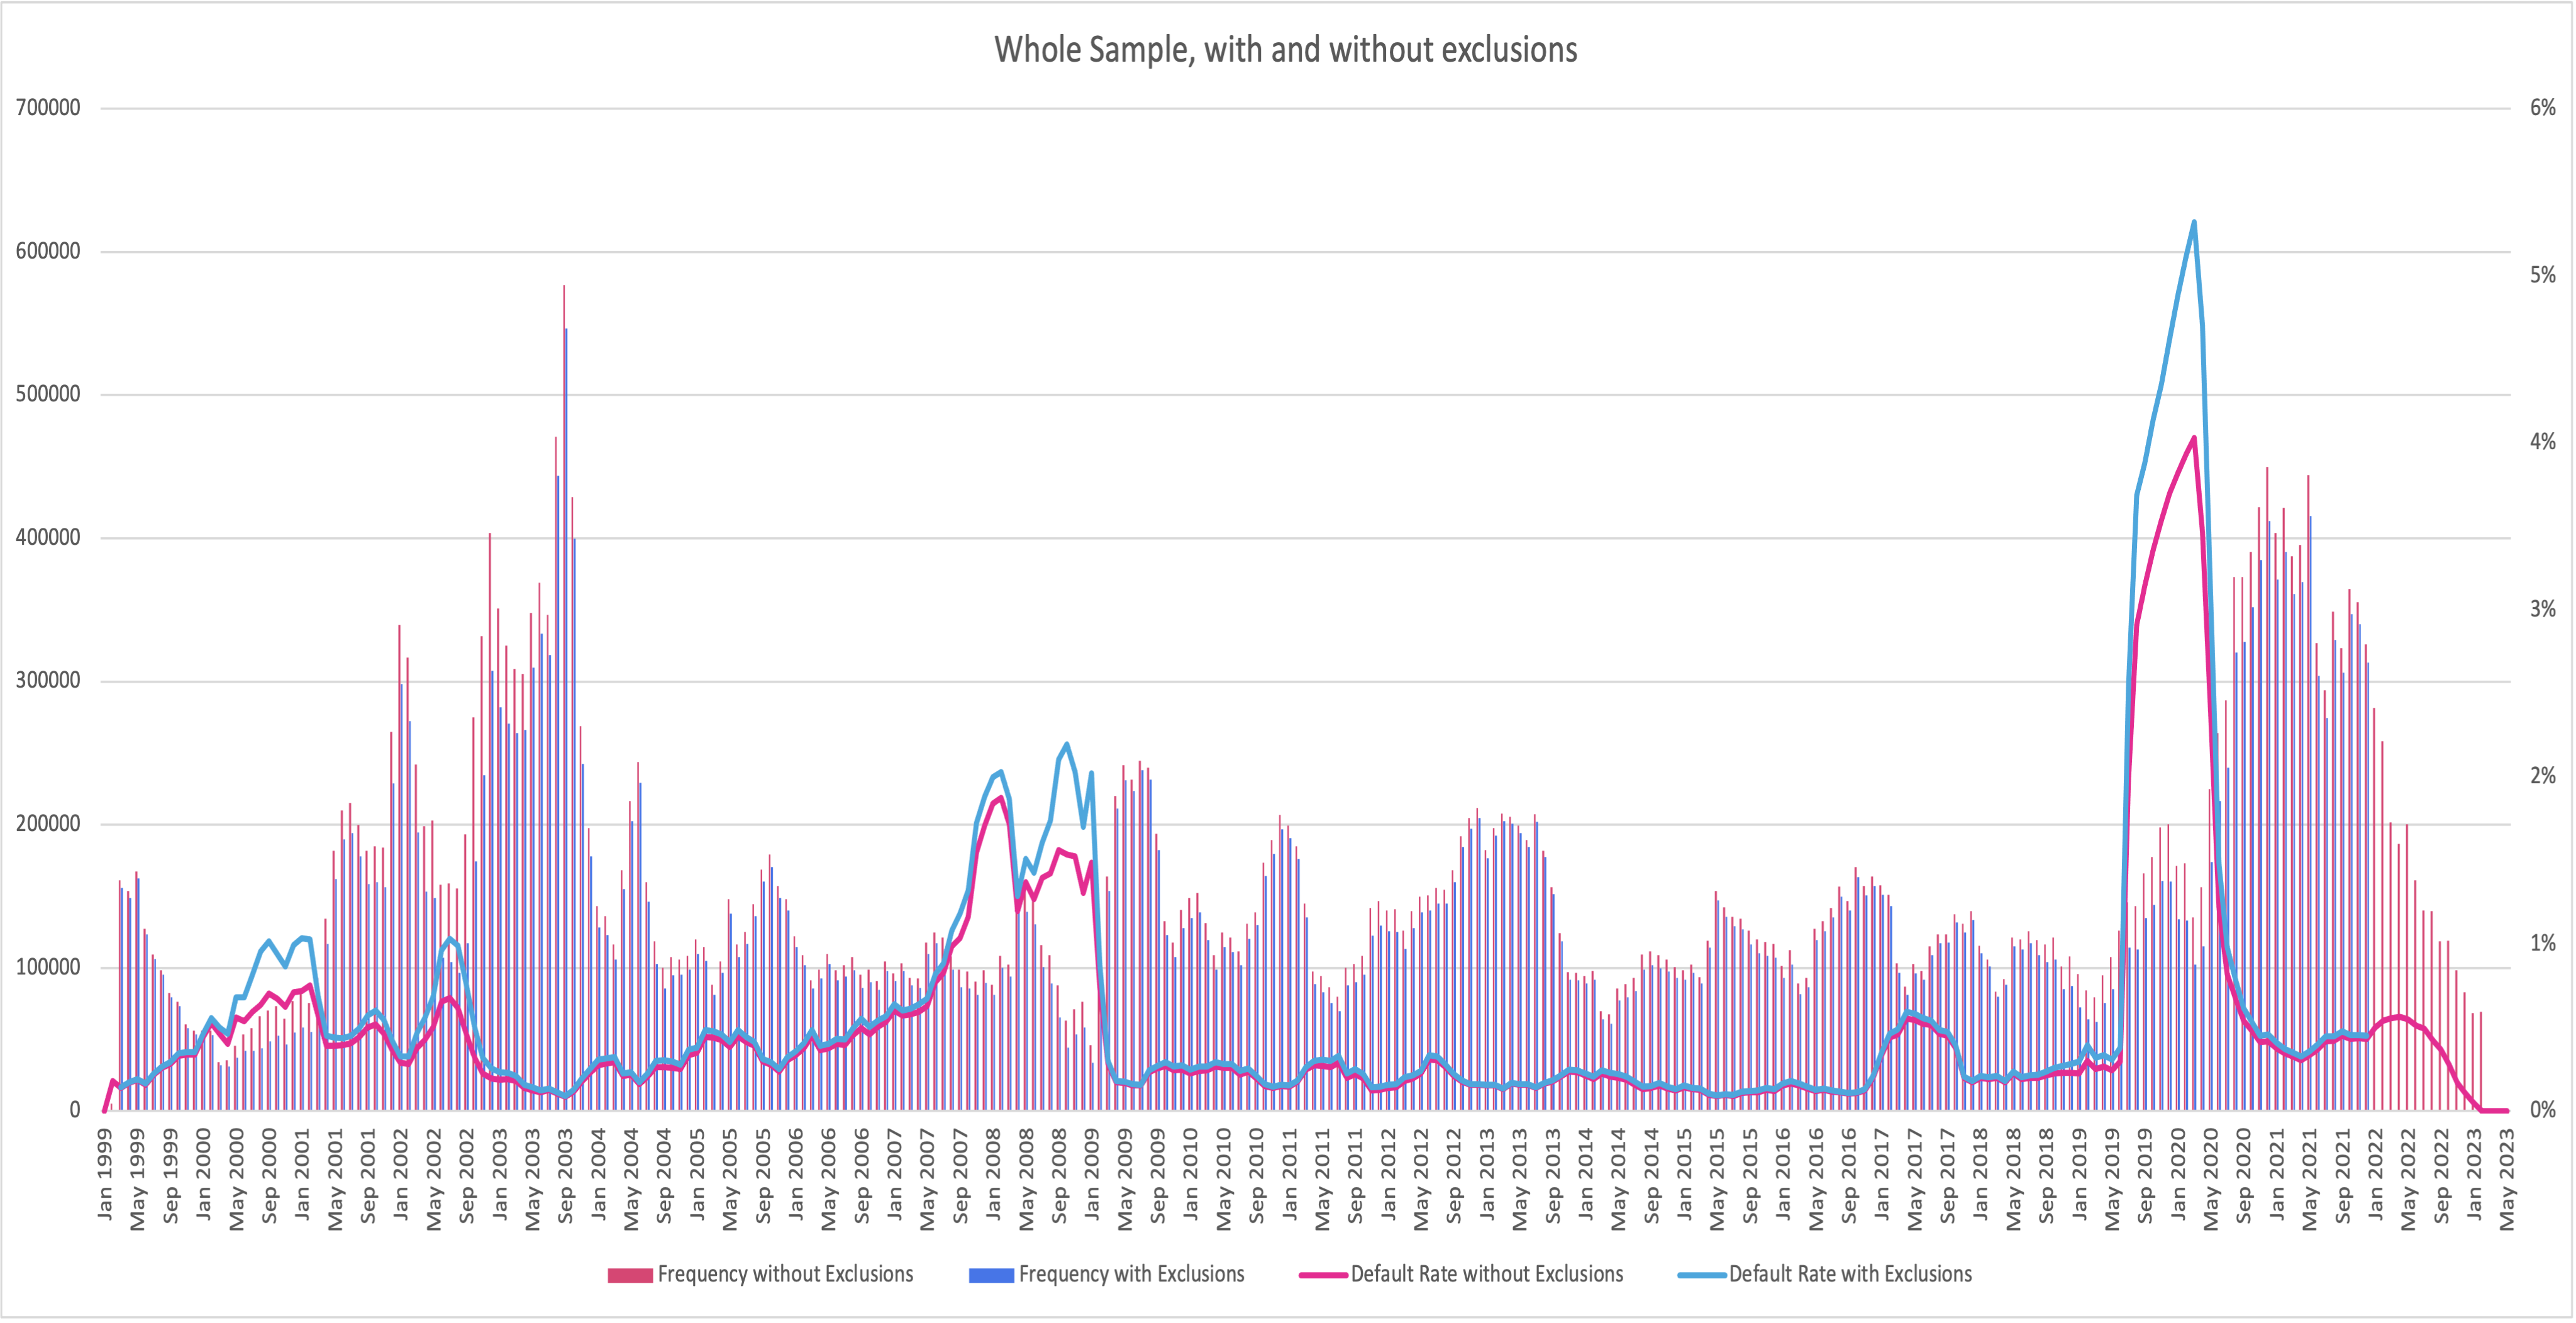
\includegraphics[width=\textwidth]{./FullSample.png}
    \caption{Default rate of whole sample}
    \label{fig:re_wholesample}
\end{figure}
\begin{figure}[H]
	\centering
	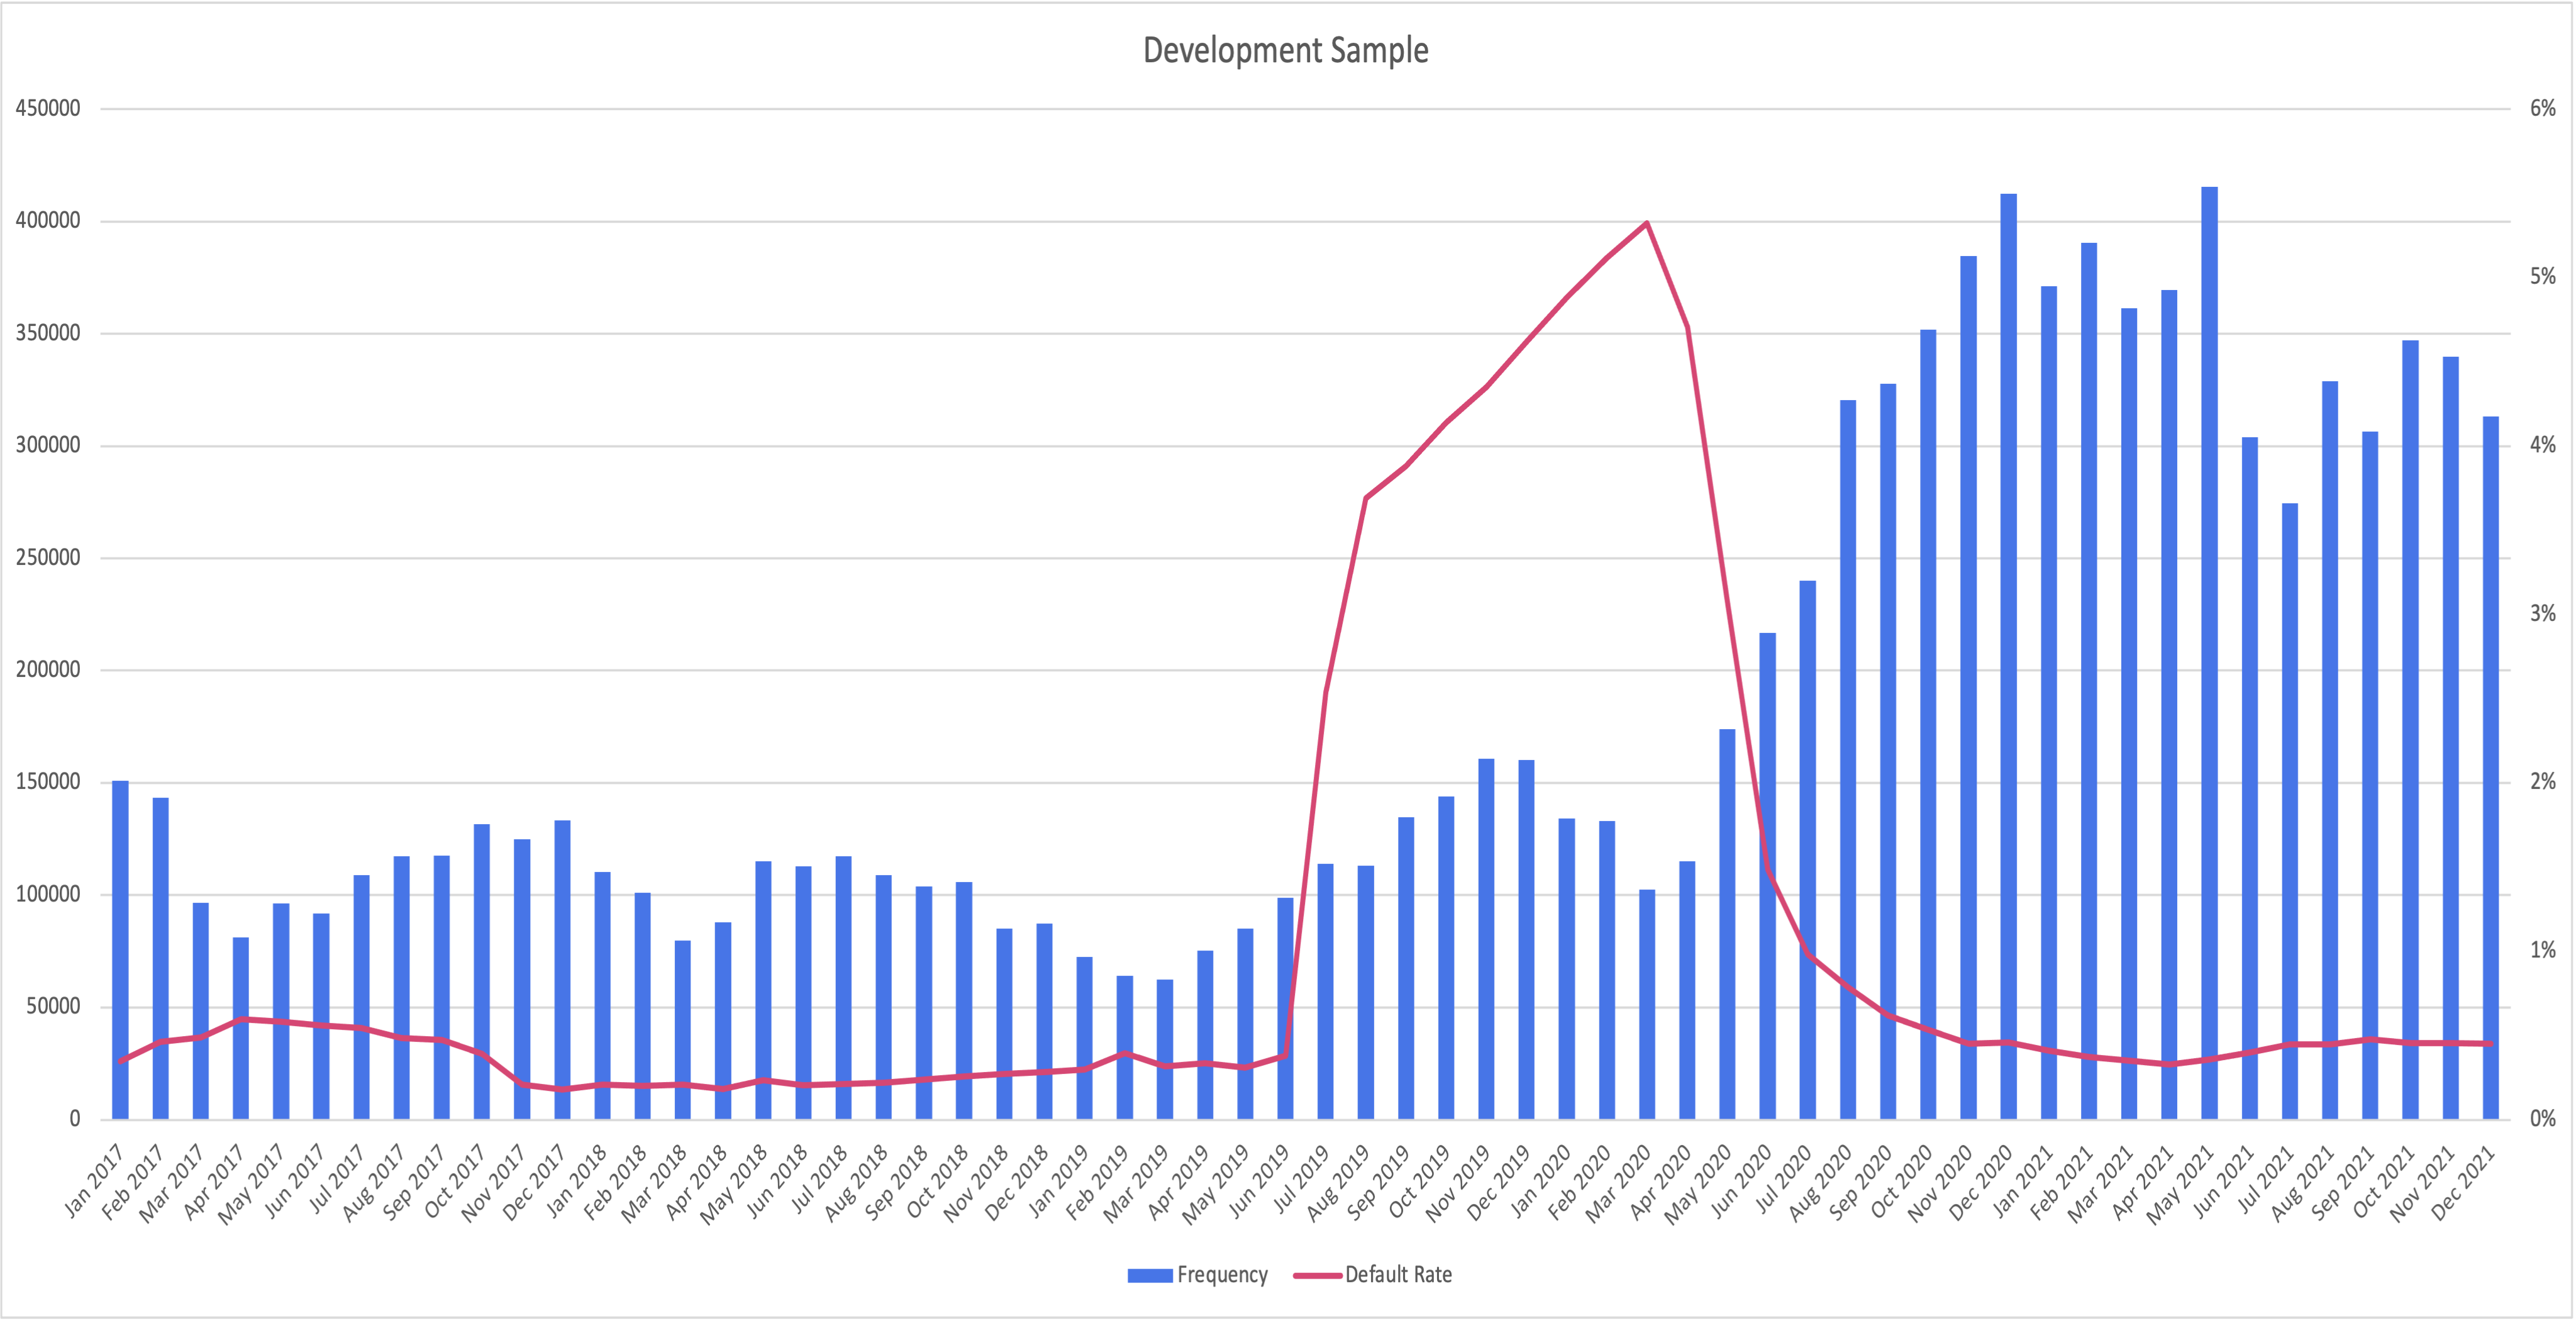
\includegraphics[width=\textwidth]{./DevelopmentSample.png}
    \caption{Distribution and default rate of development and validation sample}
    \label{fig:re_devsample}
\end{figure}

\section{Data preparation}
\subsection{Missing and Erroneous Data Treatment}
The variables were first split into three types: categorical, indicator/binary and numerical variables. All variables' missing rate were determined and given in Table \ref{tab:re_discr_power}. \emph{Program Indicator}, \emph{HARP Indicator} and \emph{Super Conforming Flag} exhibit a high proportion of missing values, exceeding 90\%, making them unsuitable for inclusion in the model. On the other hand, all other risk factors either have no missing values or possess an acceptable rate of less than 20\%. Given the low number of missing values for numerical variables such as \emph{DTI} and \emph{Credit Score} and others with a missing rate below the third decimal, imputation was performed using the median, as stated in Table \ref{tab:re_descr_stat}. Missing data points for the variable \emph{Property Valuation Method} and other categorical risk factors were treated as a distinct category while missing values for indicator variables were assigned a value of 'Y'.

No treatment of erroneous data was undertaken, as data entries outside pre-defined ranges were already set as 'Not Available' or '999' by Freddie Mac. Consequently, further analysis for potential errors was deemed unnecessary.
Figures \ref{fig:re_distr1} to \ref{fig:re_distr4} show the distribution plots of relevant risk factors; all plots are given in Appendix \ref{sec:distr_all}.

\begin{figure}[H]
\begin{minipage}{.5\textwidth}
	\centering
	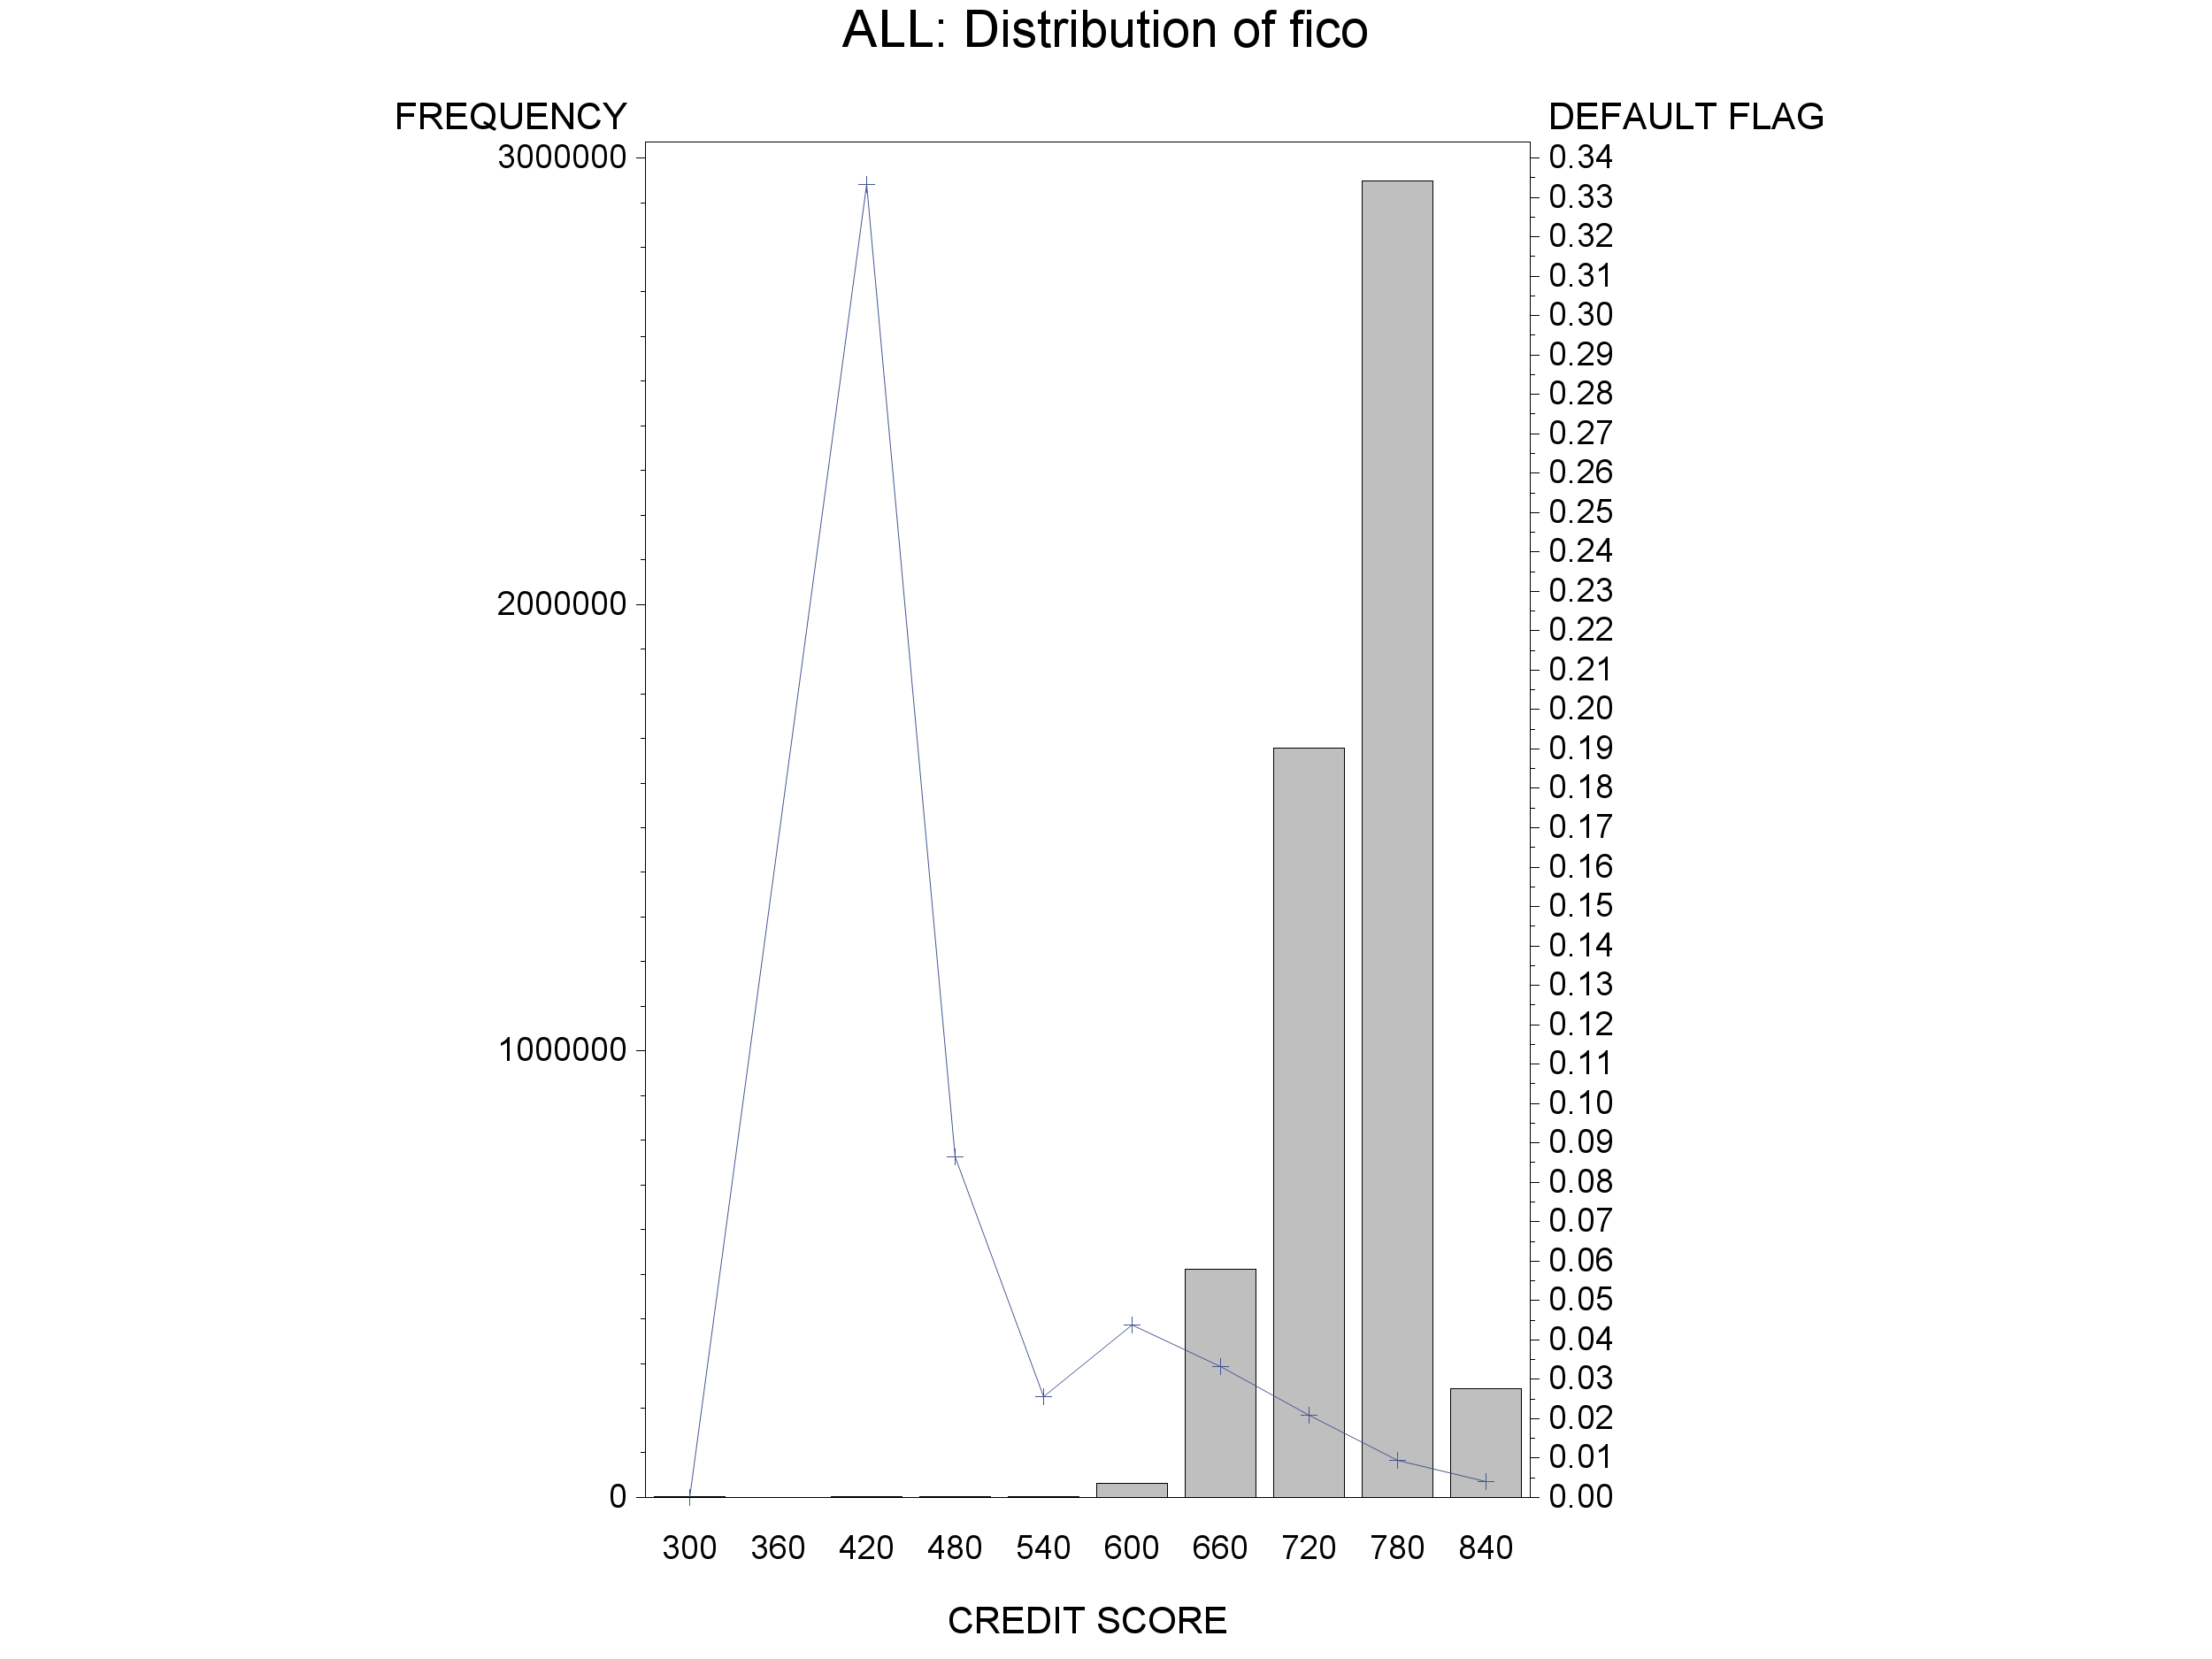
\includegraphics[width=0.9\textwidth]{./plot/Distribution/Main/RE_NUM_fico_DISTRIBUTION_ALL.png}
\end{minipage}%
\begin{minipage}{.5\textwidth}
	\centering
	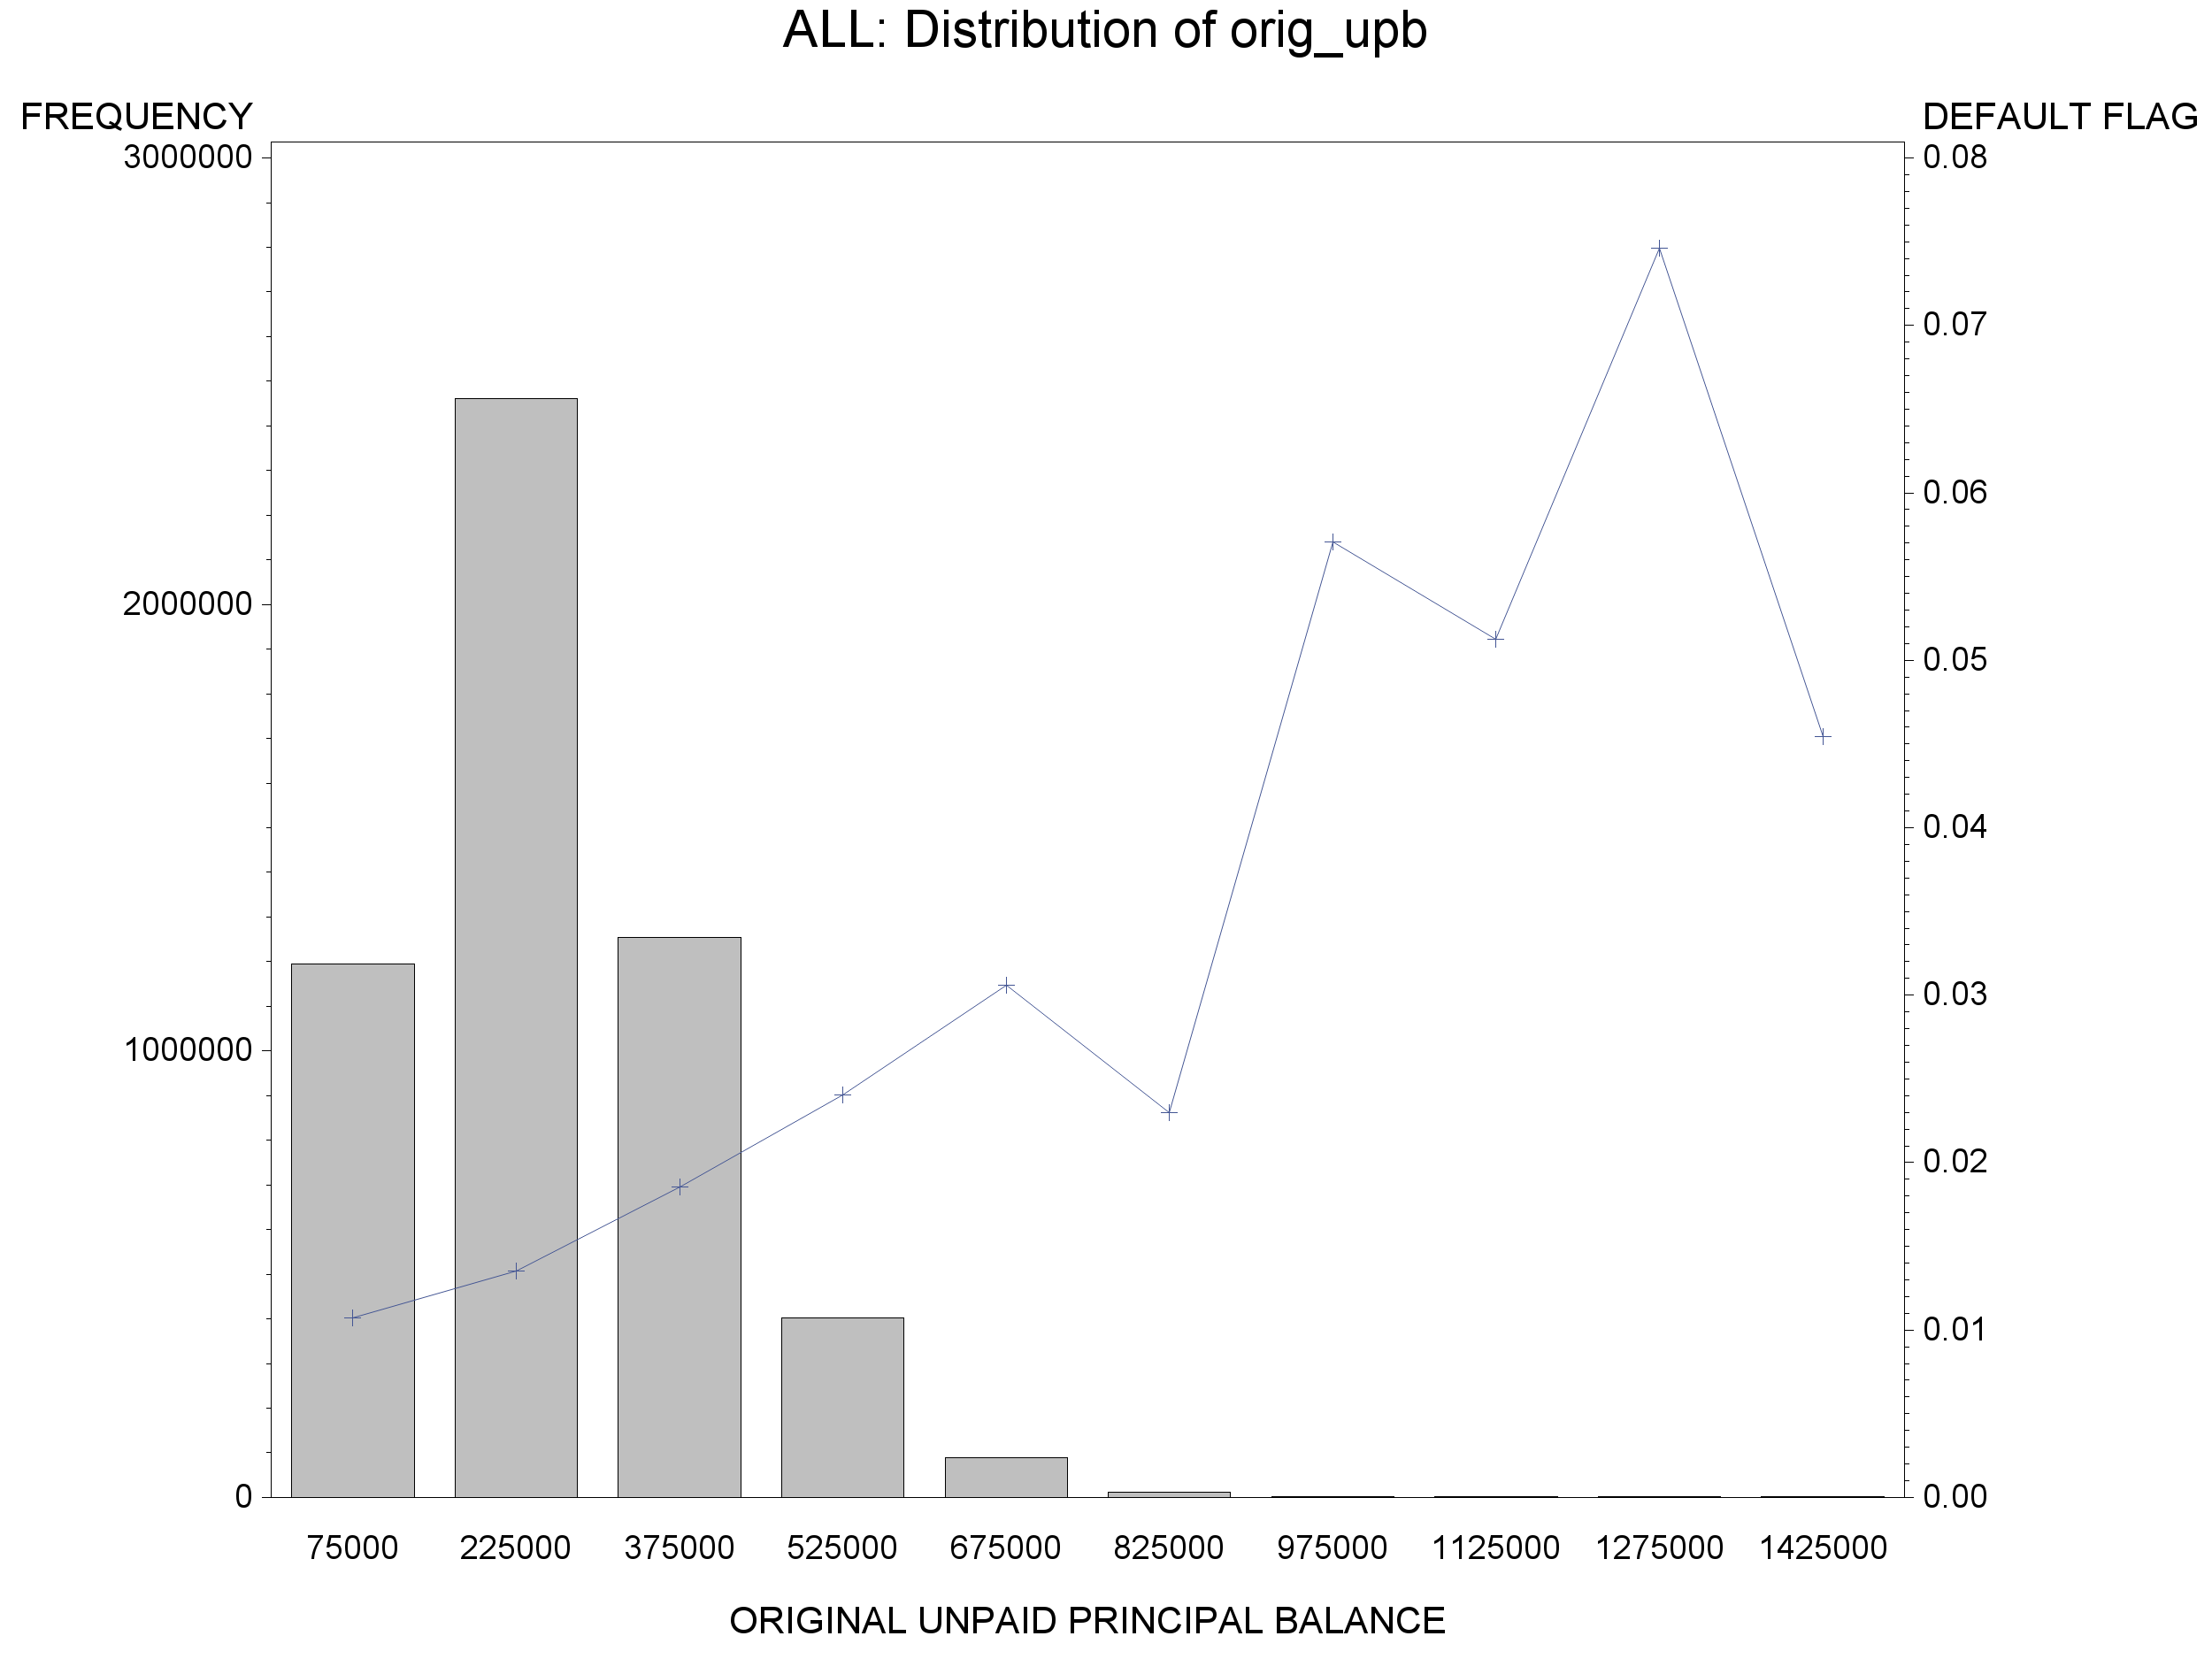
\includegraphics[width=0.9\textwidth]{./plot/Distribution/Main/RE_NUM_orig_upb_DISTRIBUTION_ALL.png}
\end{minipage}
    \caption{Distribution of Credit Score (fico) and Original UPB}
    \label{fig:re_distr1}
\end{figure}
\begin{figure}[H]
\begin{minipage}{.5\textwidth}
	\centering
	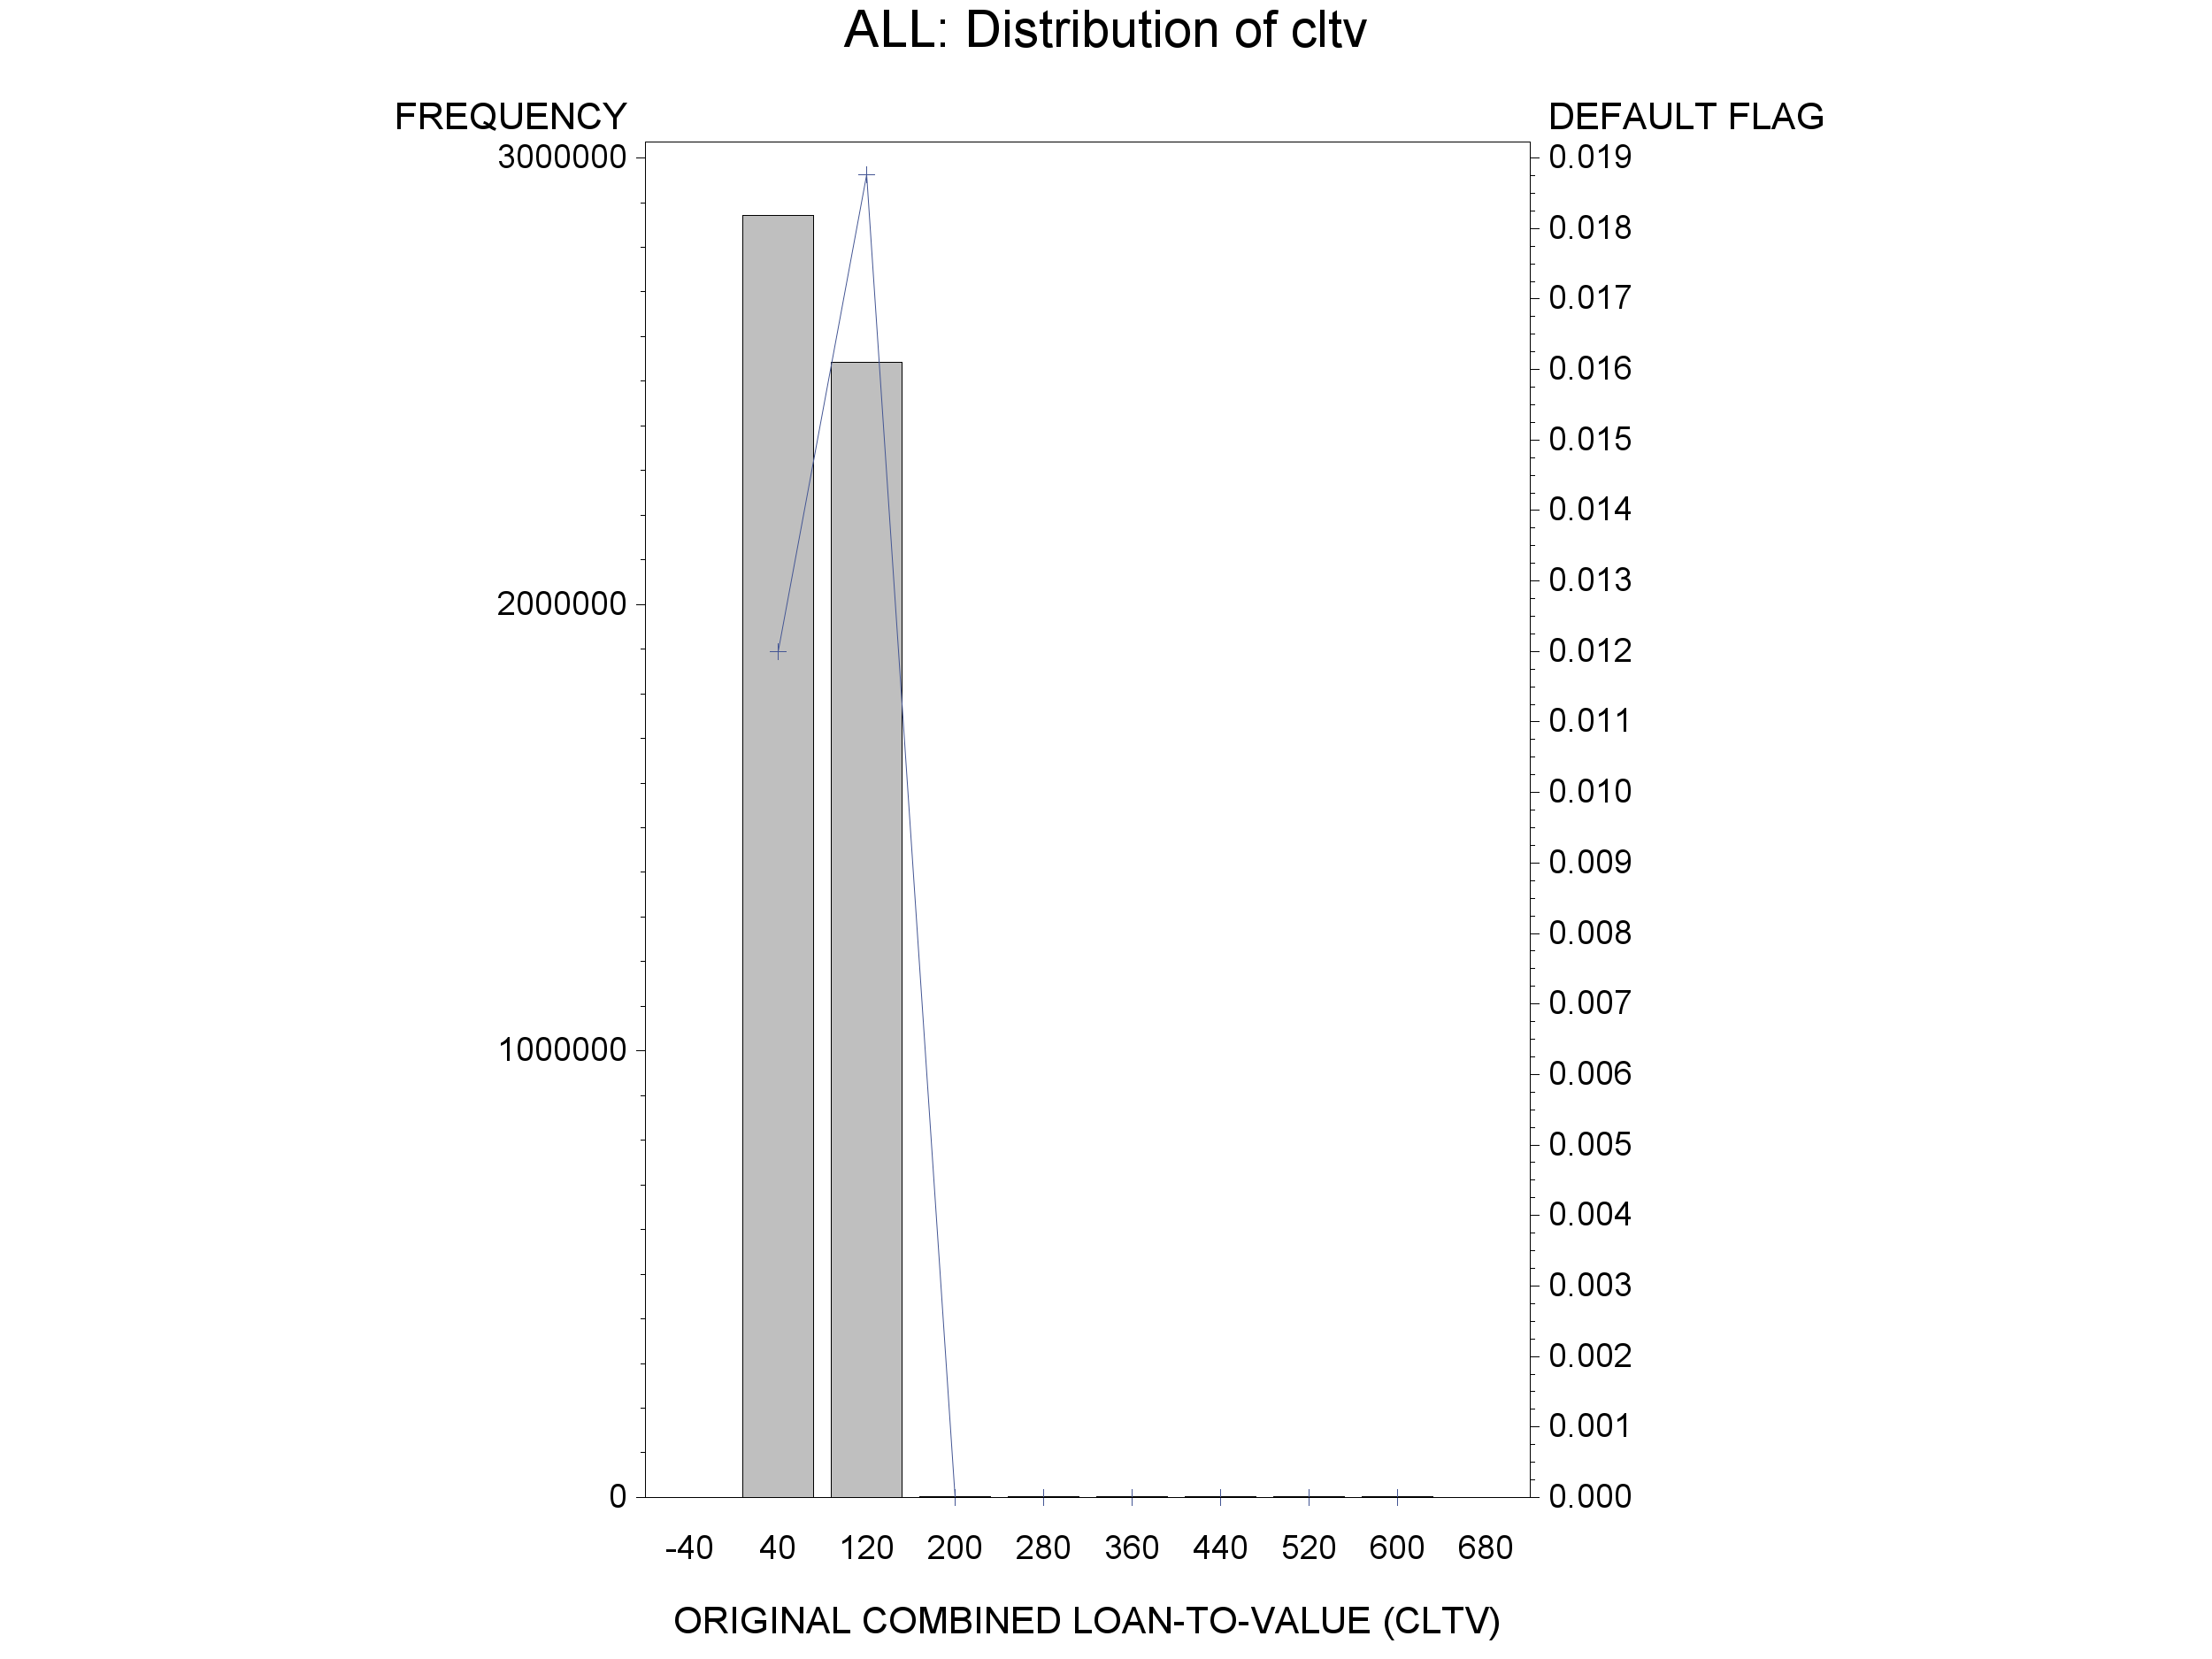
\includegraphics[width=0.9\textwidth]{./plot/Distribution/Main/RE_NUM_cltv_DISTRIBUTION_ALL.png}
\end{minipage}%
\begin{minipage}{.5\textwidth}
	\centering
	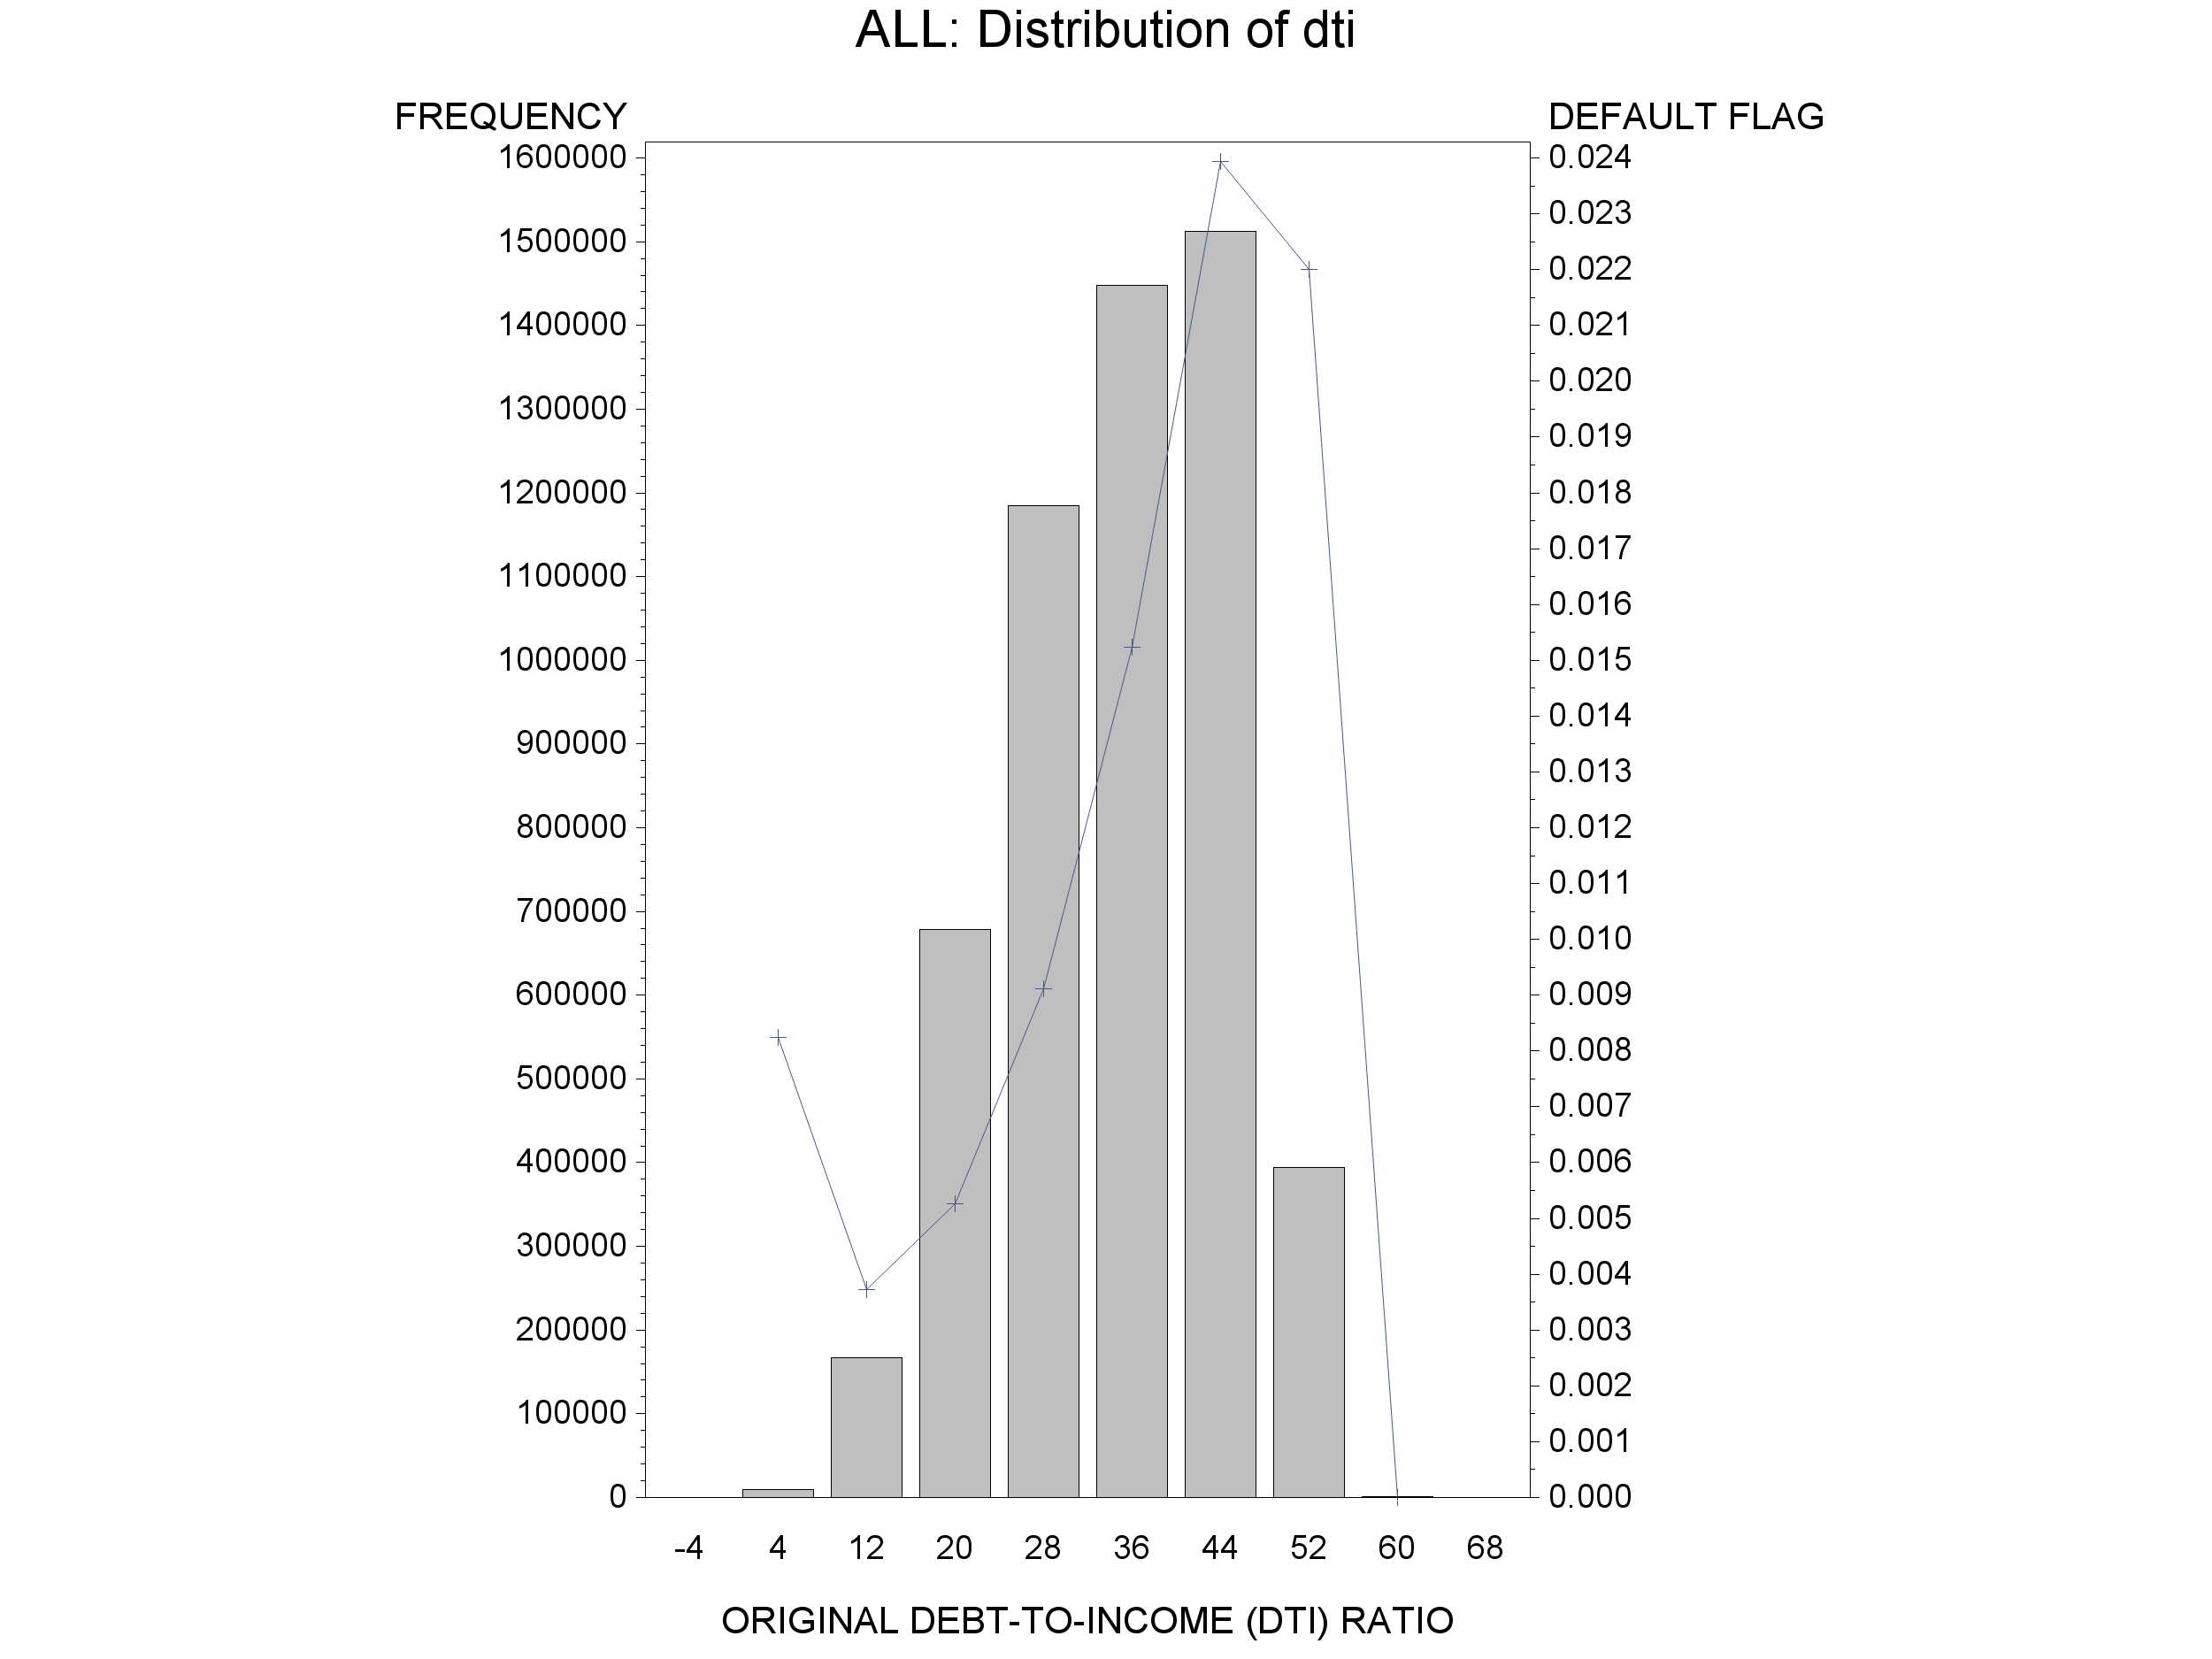
\includegraphics[width=0.9\textwidth]{./plot/Distribution/Main/RE_NUM_dti_DISTRIBUTION_ALL.png}
\end{minipage}
    \caption{Distribution of CLTV and DTI}
    %\label{fig:dp_iqr_boxpl}
\end{figure}
\begin{figure}[H]
\begin{minipage}{.5\textwidth}
	\centering
	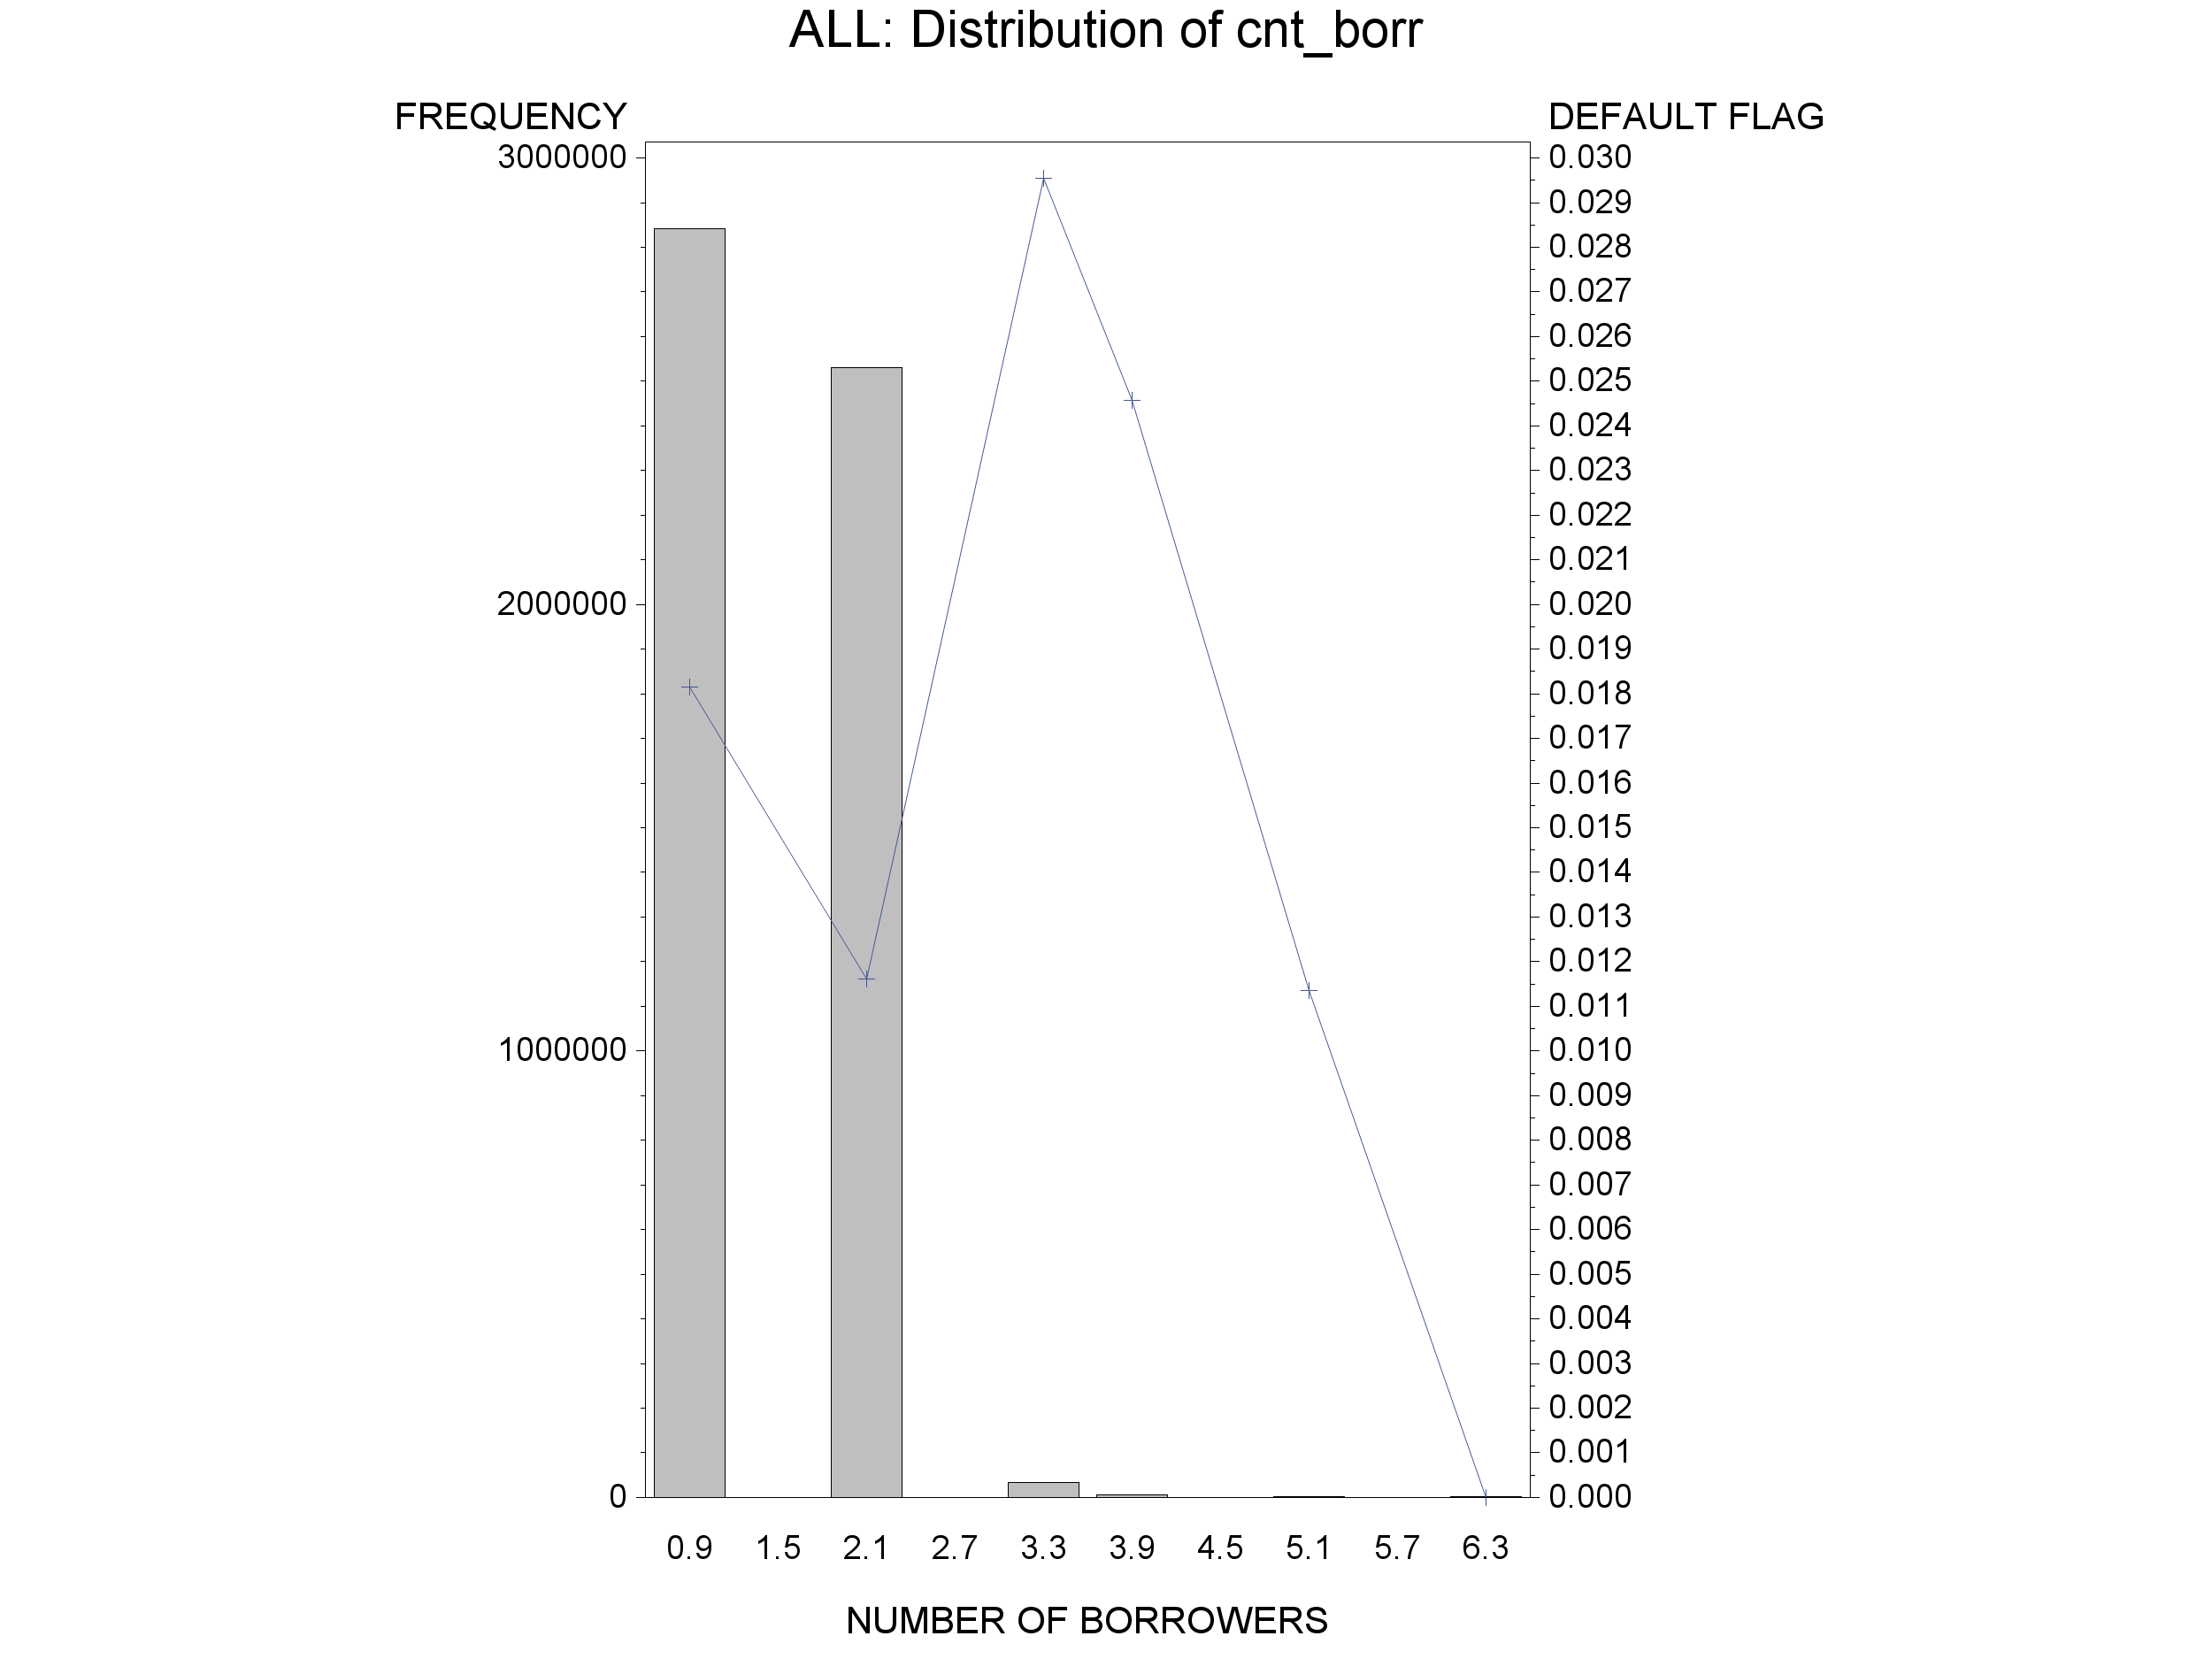
\includegraphics[width=0.9\textwidth]{./plot/Distribution/Main/RE_NUM_cnt_borr_DISTRIBUTION_ALL.png}
\end{minipage}%
\begin{minipage}{.5\textwidth}
	\centering
	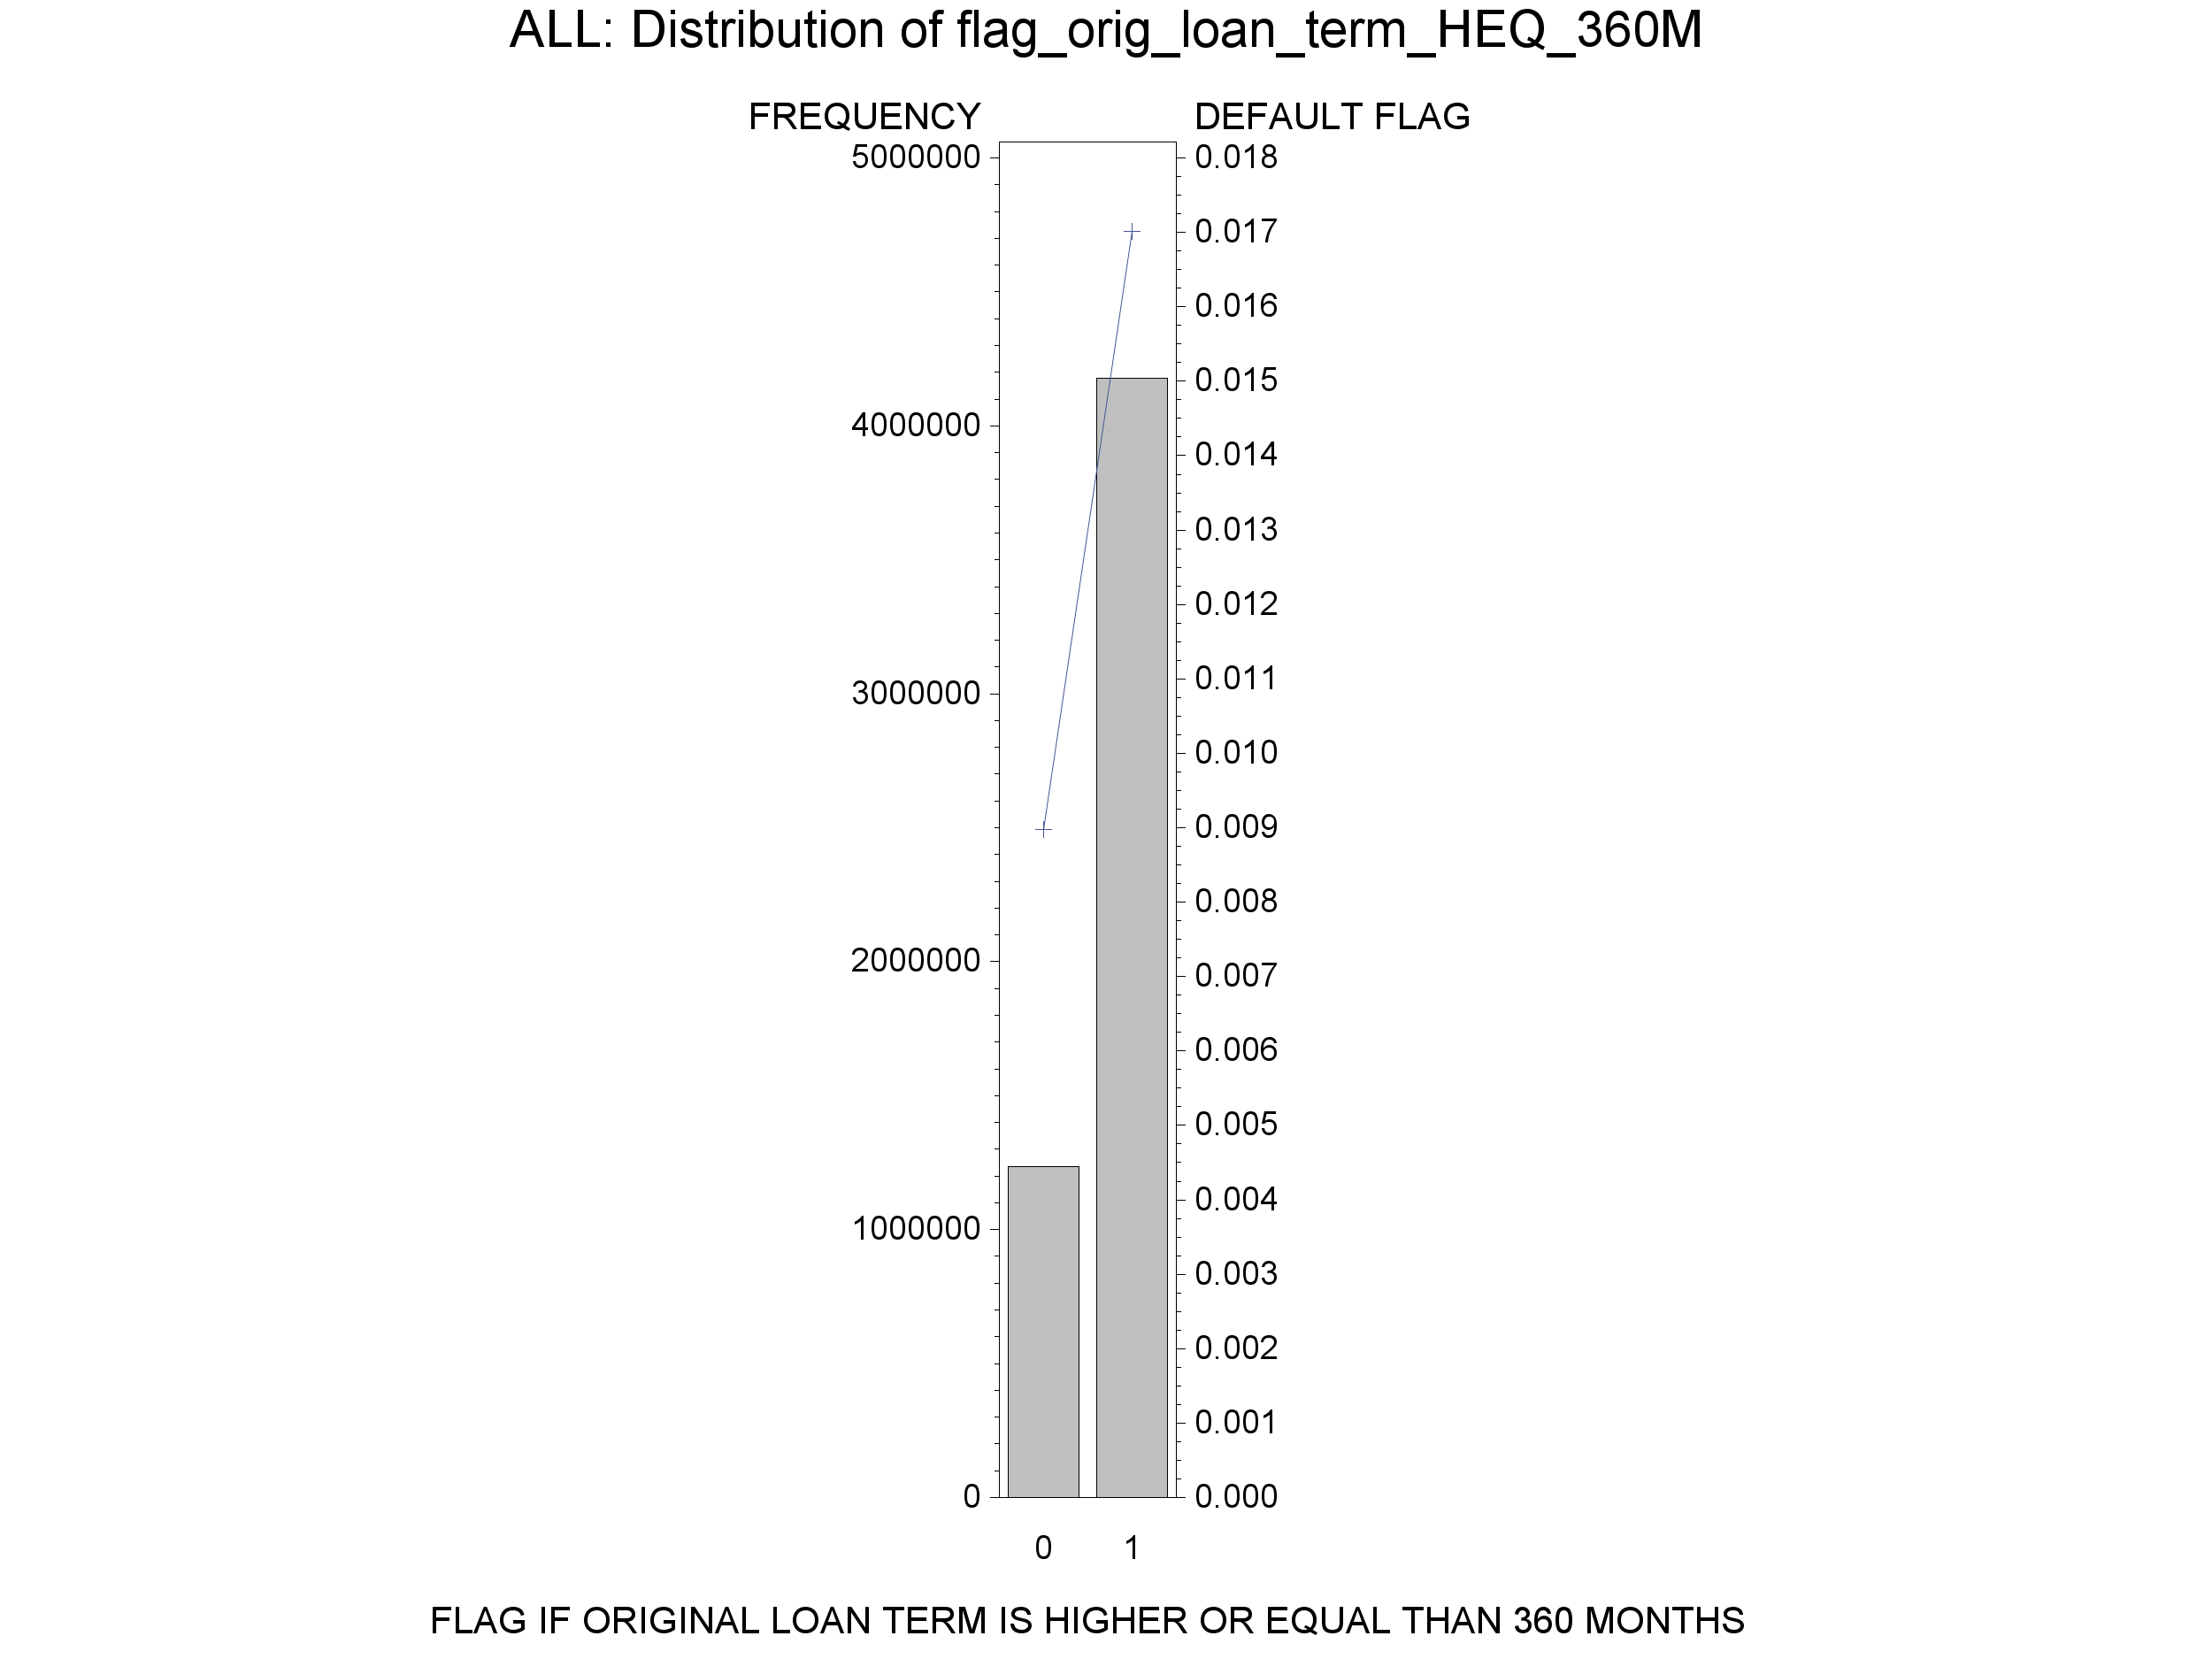
\includegraphics[width=0.9\textwidth]{./plot/Distribution/Main/RE_IND_flag_orig_loan_term_HEQ_360M_DISTRIBUTION_ALL.png}
\end{minipage}
    \caption{Distribution of Number of borrowers and Flag Original Loan Term $\geq$ 360 months}
    %\label{fig:dp_iqr_boxpl}
\end{figure}
\begin{figure}[H]
\begin{minipage}{.5\textwidth}
	\centering
	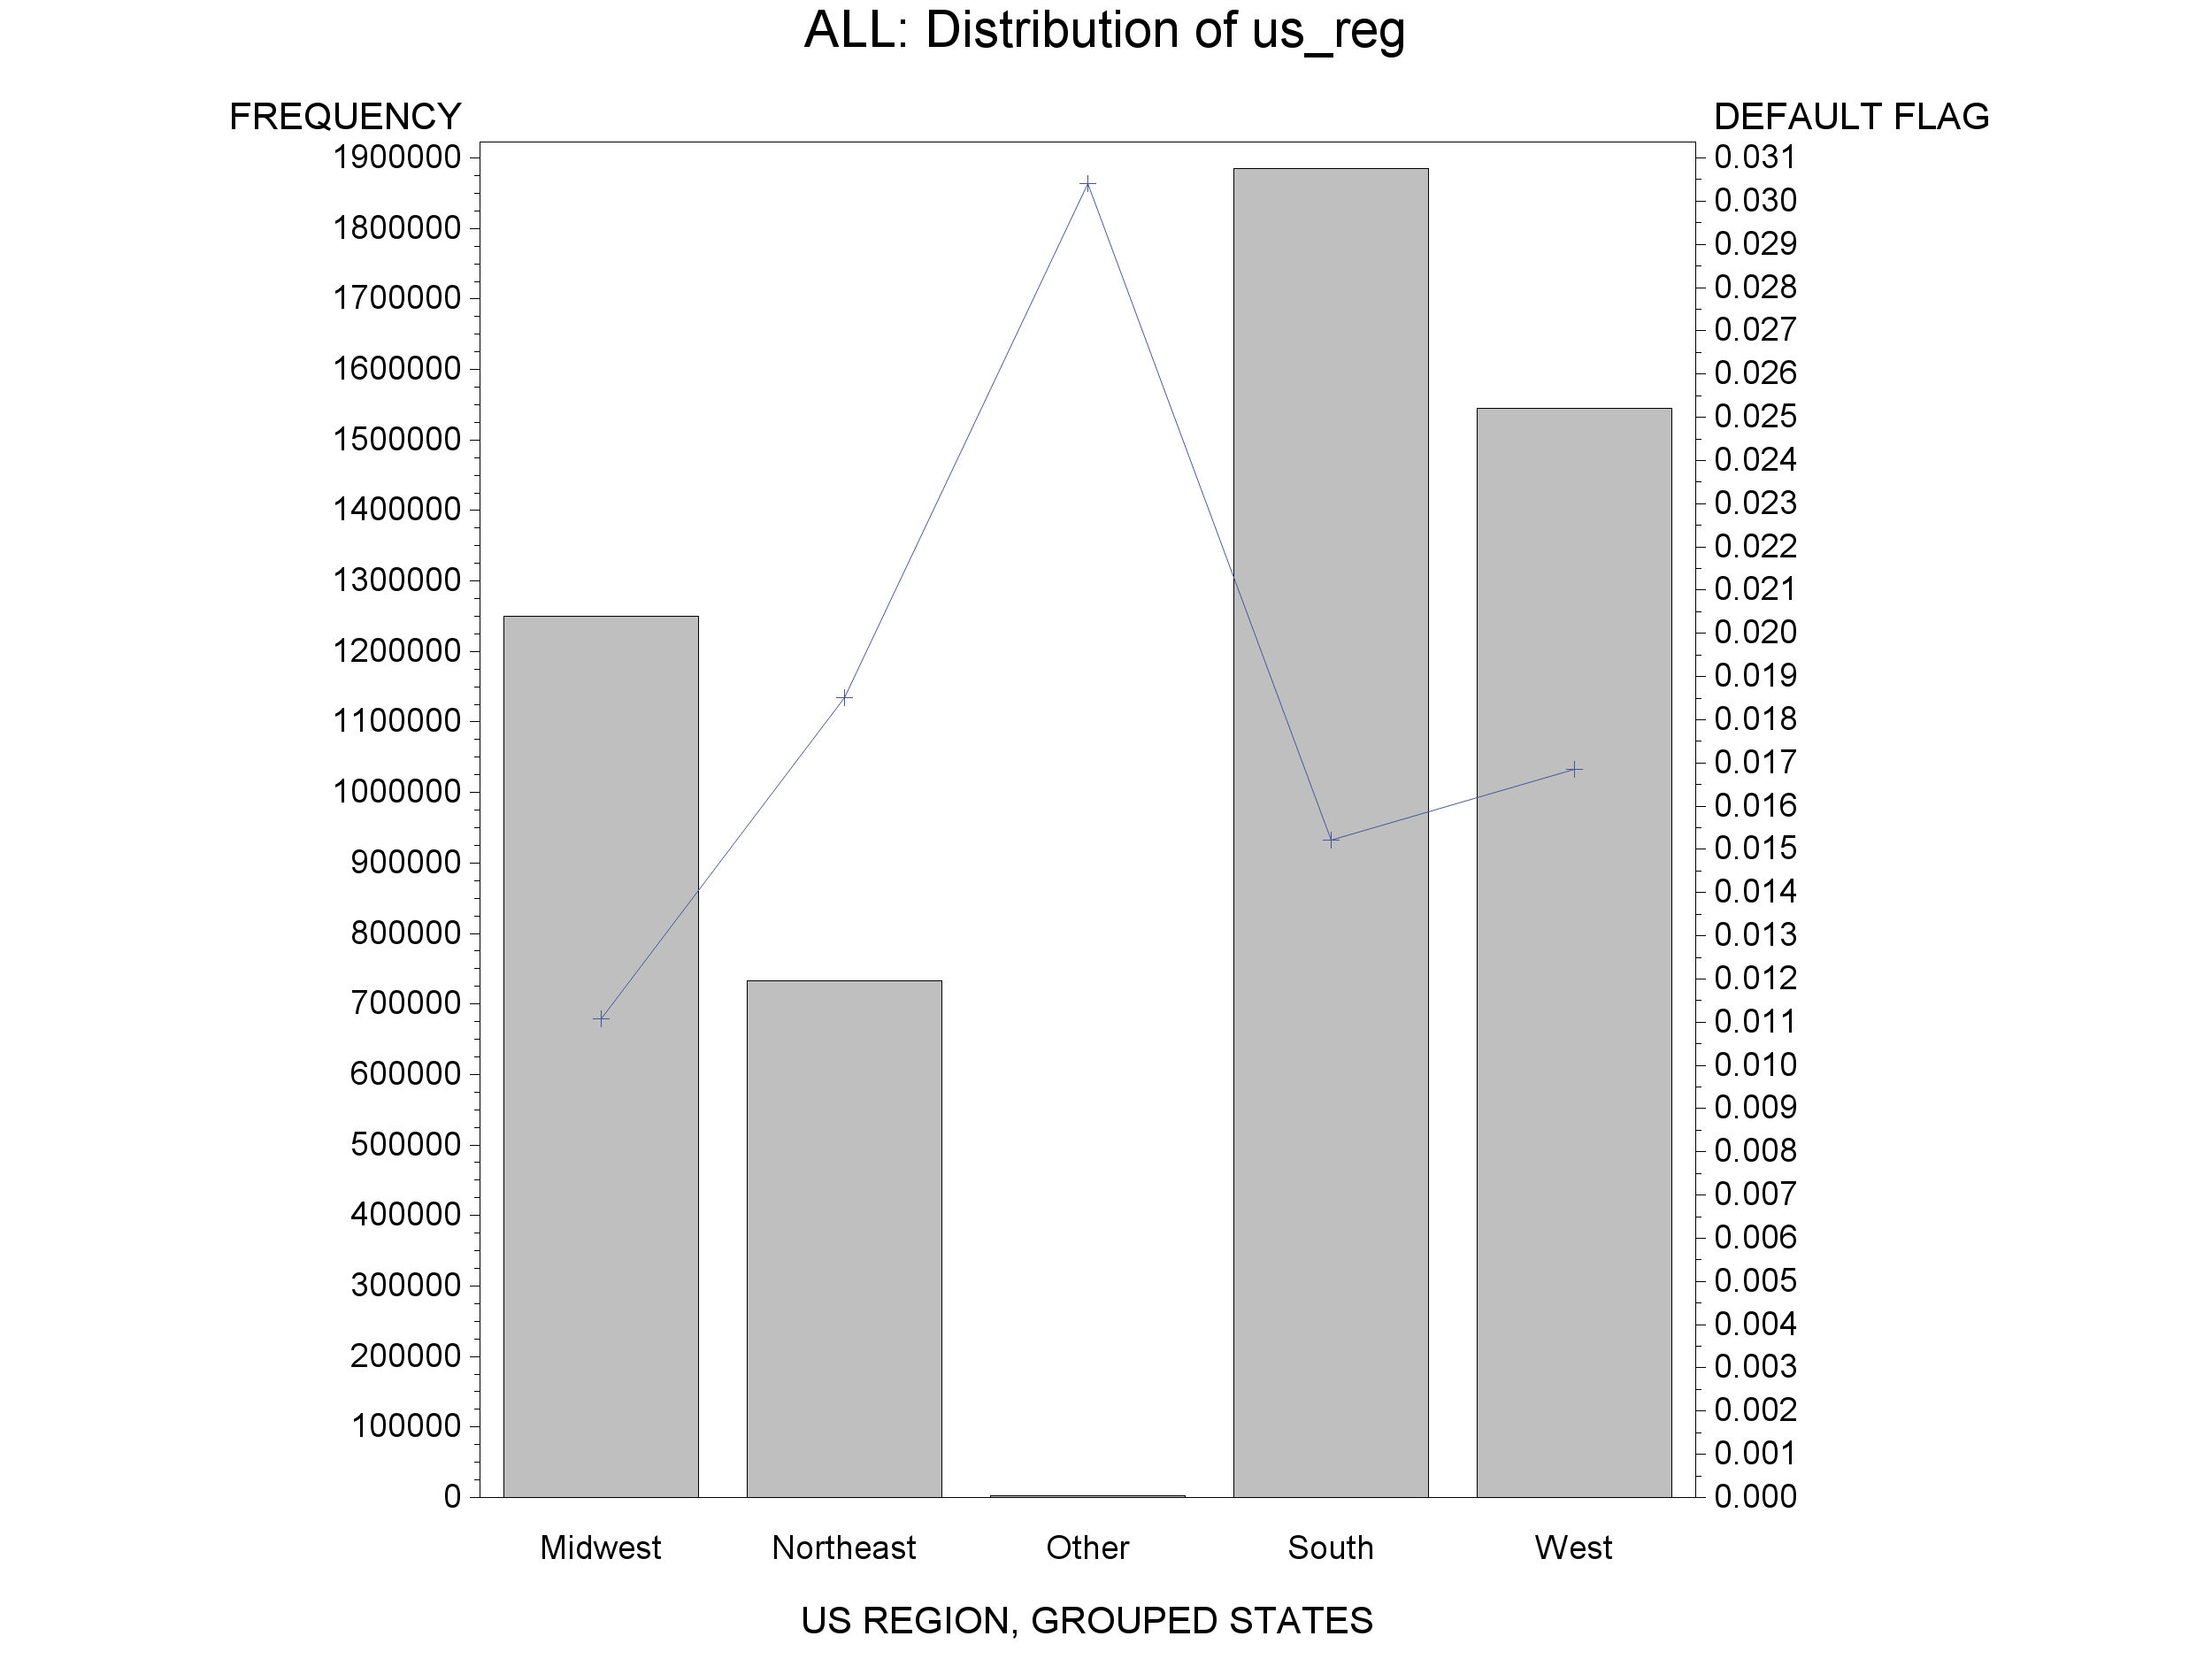
\includegraphics[width=0.9\textwidth]{./plot/Distribution/Main/RE_CAT_us_reg_DISTRIBUTION_ALL.png}
\end{minipage}%
\begin{minipage}{.5\textwidth}
	\centering
	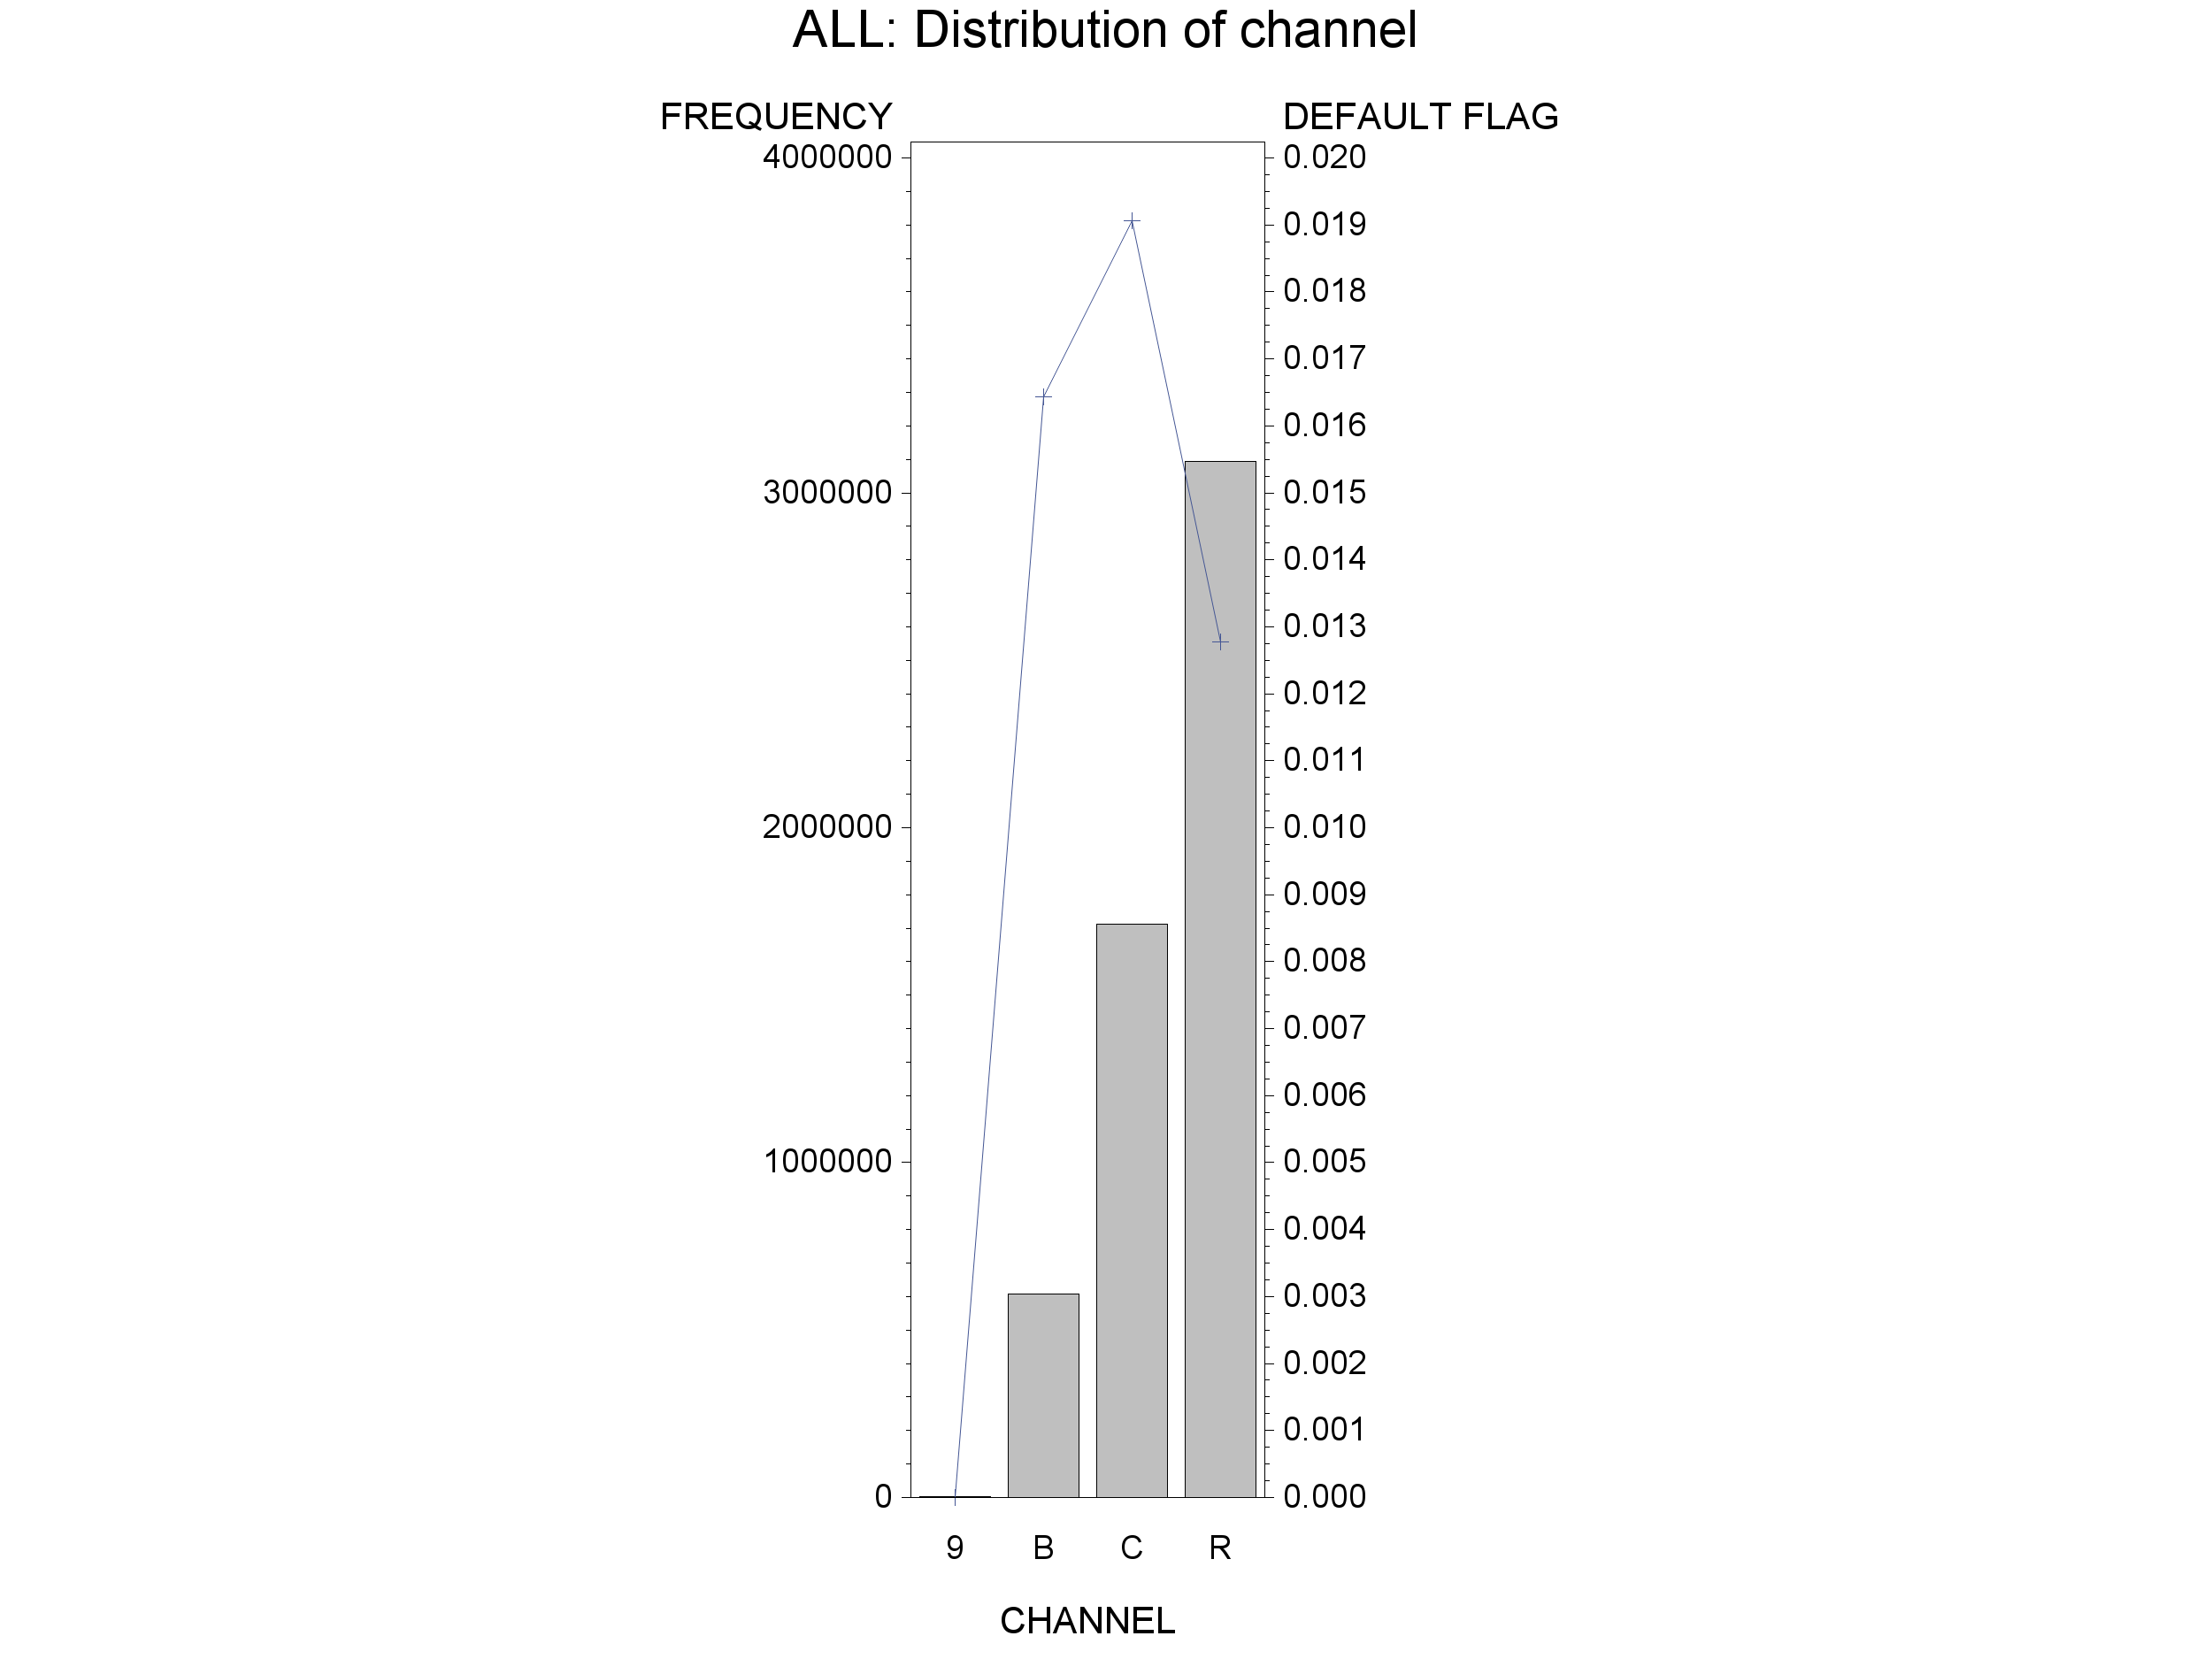
\includegraphics[width=0.9\textwidth]{./plot/Distribution/Main/RE_CAT_channel_DISTRIBUTION_ALL.png}
\end{minipage}
    \caption{Distribution of US region and Channel}
    \label{fig:re_distr4}
\end{figure}

\subsection{Outlier Treatment}
The interquartile approach, detailed in Chapter \ref{sec:OutlTr}, was employed to identify outliers and their presentation was visualized through boxplots (Figure \ref{fig:re_boxpl_fico_origupb} - \ref{fig:re_boxpl_noborr_loanterm}, all plots in Appendix \ref{sec:boxplot_all}). Upper and lower boundaries were determined using Equations \ref{eq:dp_iqr_boxpl2} and \ref{eq:dp_iqr_boxpl2}. Quartiles for all numerical risk factors are outlined in Table \ref{tab:re_descr_stat}, with resulting limits available in Table \ref{tab:re_iqr}. The proportion of upper and lower outliers was calculated to analyze if a significant amount of data entries were affected and could potentially impact the modeling process. While outliers were present in all numerical variables, only the risk factor \emph{Original Loan Term} shows a concerning proportion. New risk factors were derived to circumvent this issue. Multiple versions of indicator variables were created using the definition listed in Table \ref{tab:re_descr_newvar}. Additionally, after analyzing the distribution and box plots of all risk factors, a winsorization was executed to evaluate if outliers affected the discriminatory power negatively. Therefore, data points with values above the upper or below the lower limit were capped at their respective thresholds. The performance of the adjusted variables did not change significantly, and thus, the original versions were retained.

\begin{figure}[H]
\begin{minipage}{.5\textwidth}
	\centering
	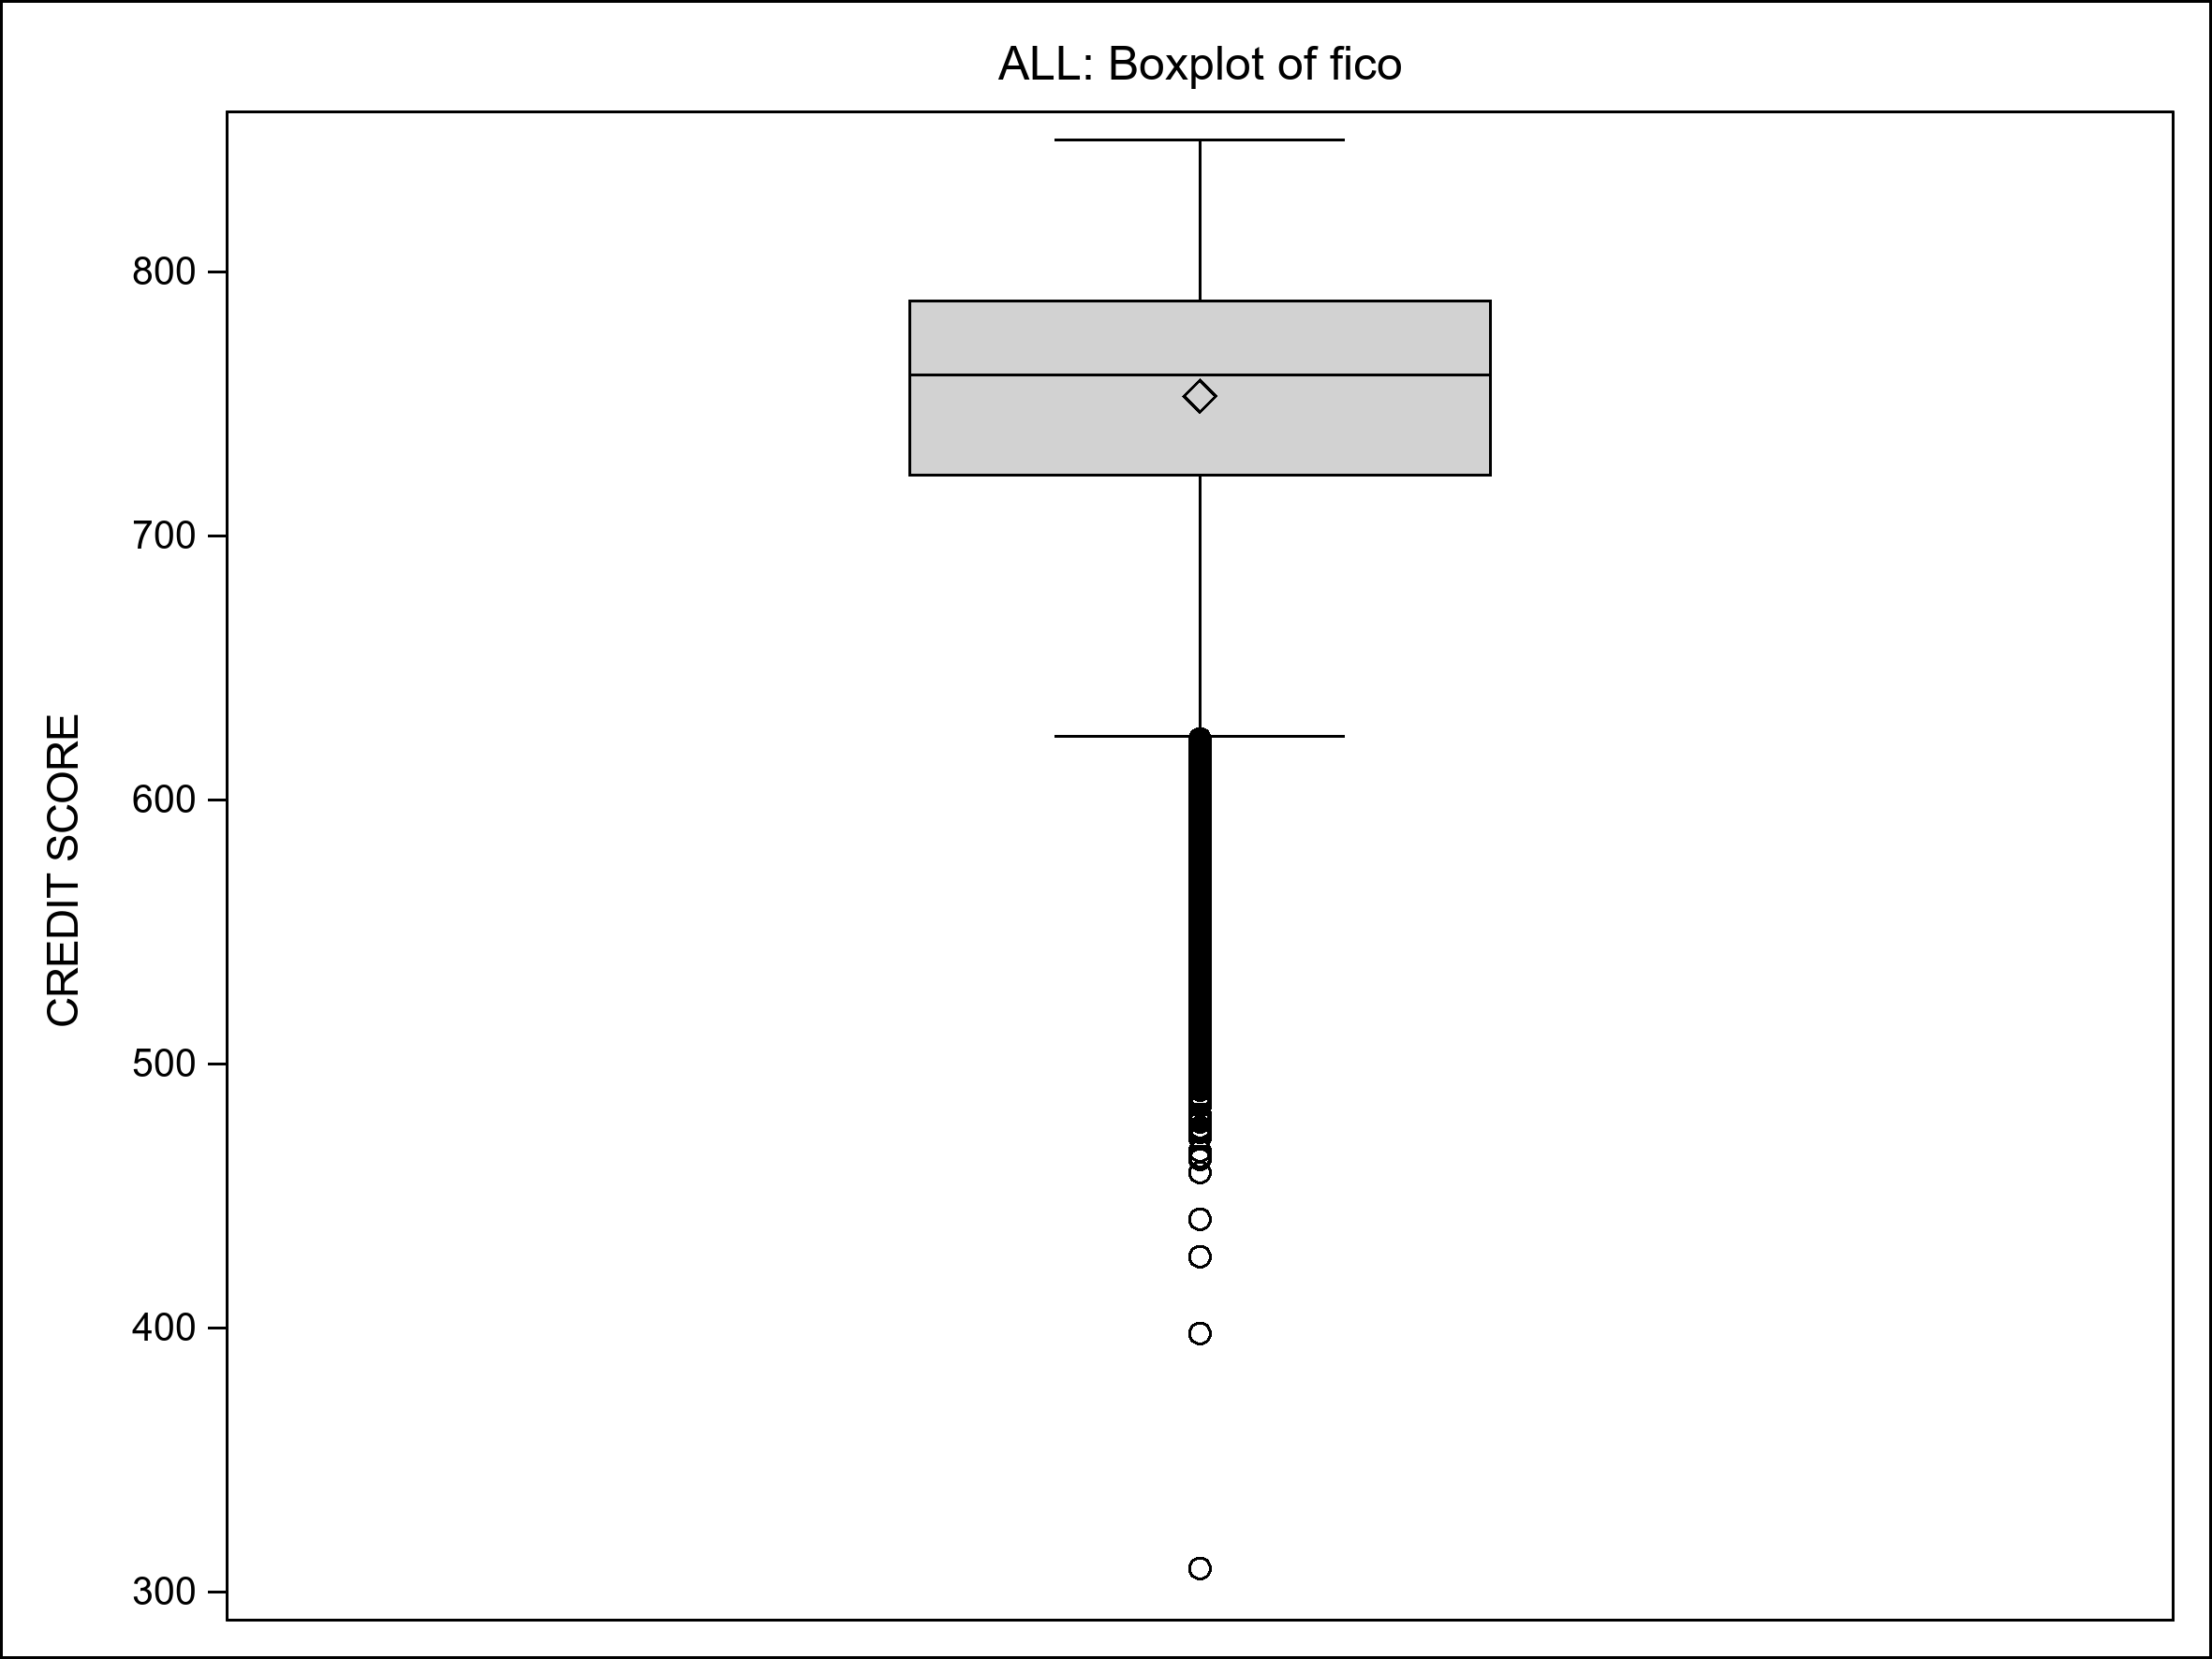
\includegraphics[width=0.9\textwidth]{./plot/Boxplot/Main/NUM_fico_BOXPLOT_ALL1.png}
\end{minipage}%
\begin{minipage}{.5\textwidth}
	\centering
	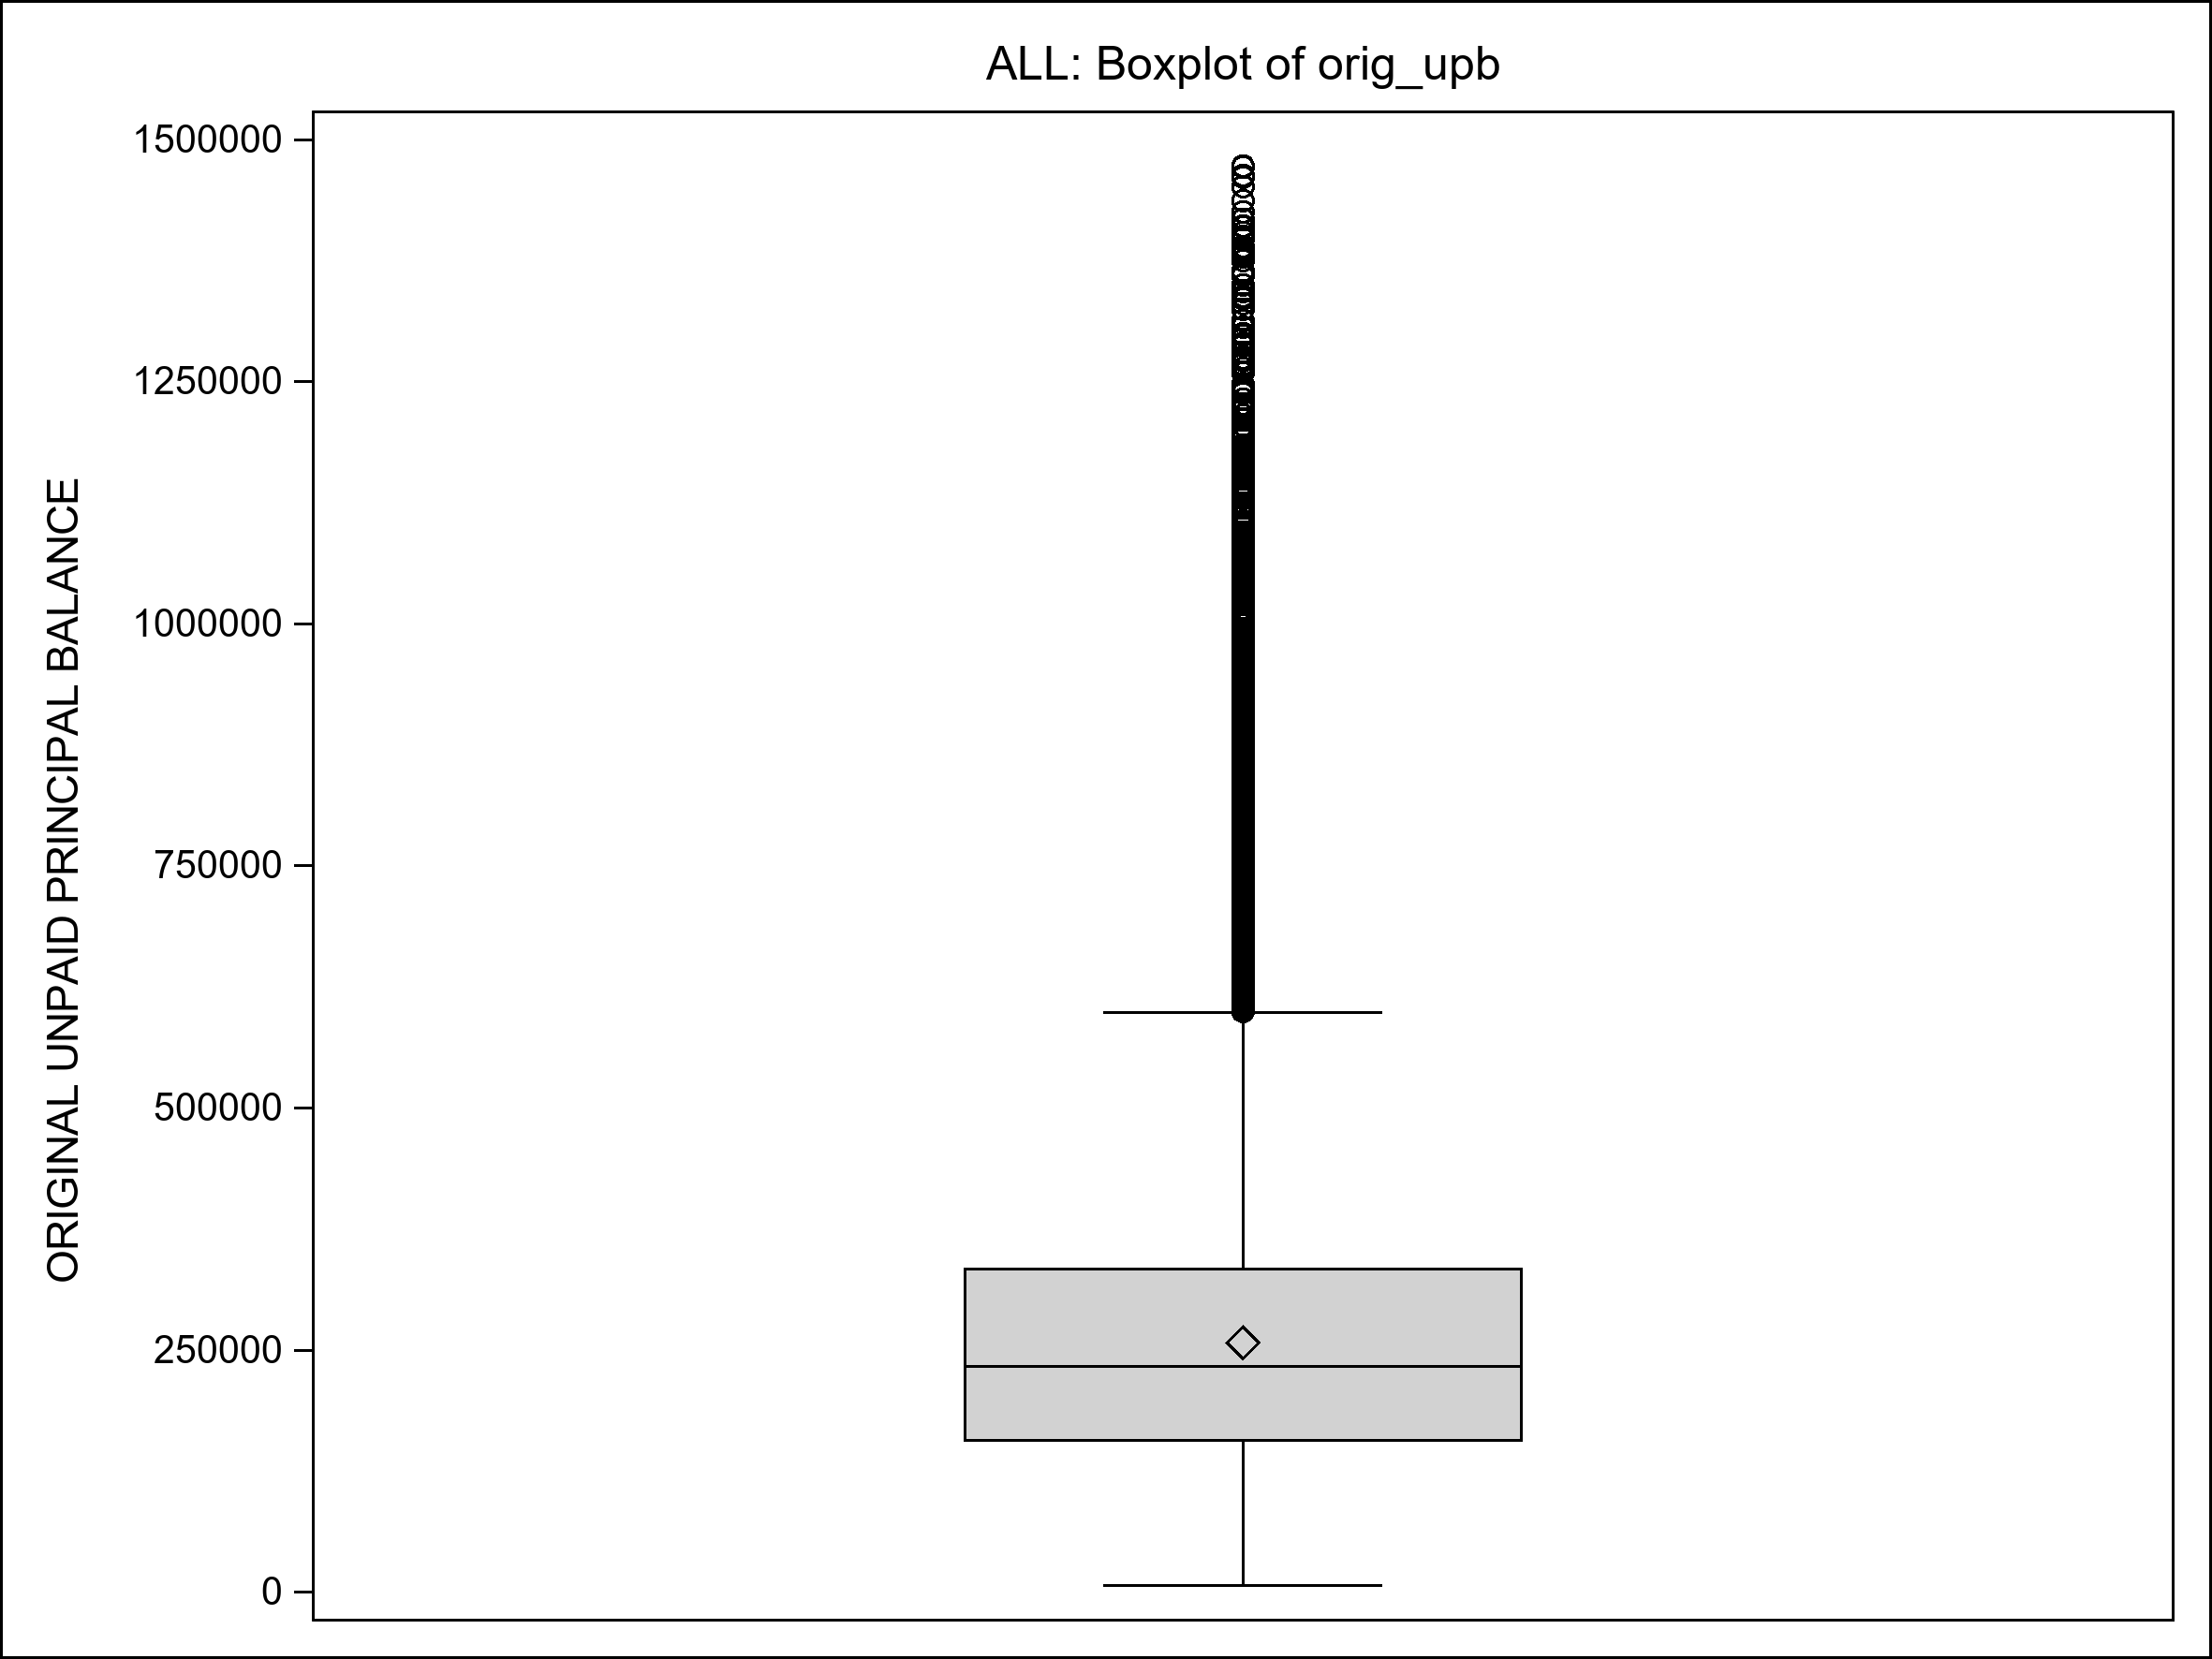
\includegraphics[width=0.9\textwidth]{./plot/Boxplot/Main/NUM_orig_upb_BOXPLOT_ALL1.png}
\end{minipage}
    \caption{Boxplot of Credit Score (fico) and Original UPB}
    \label{fig:re_boxpl_fico_origupb}
\end{figure}
\begin{figure}[H]
\begin{minipage}{.5\textwidth}
	\centering
	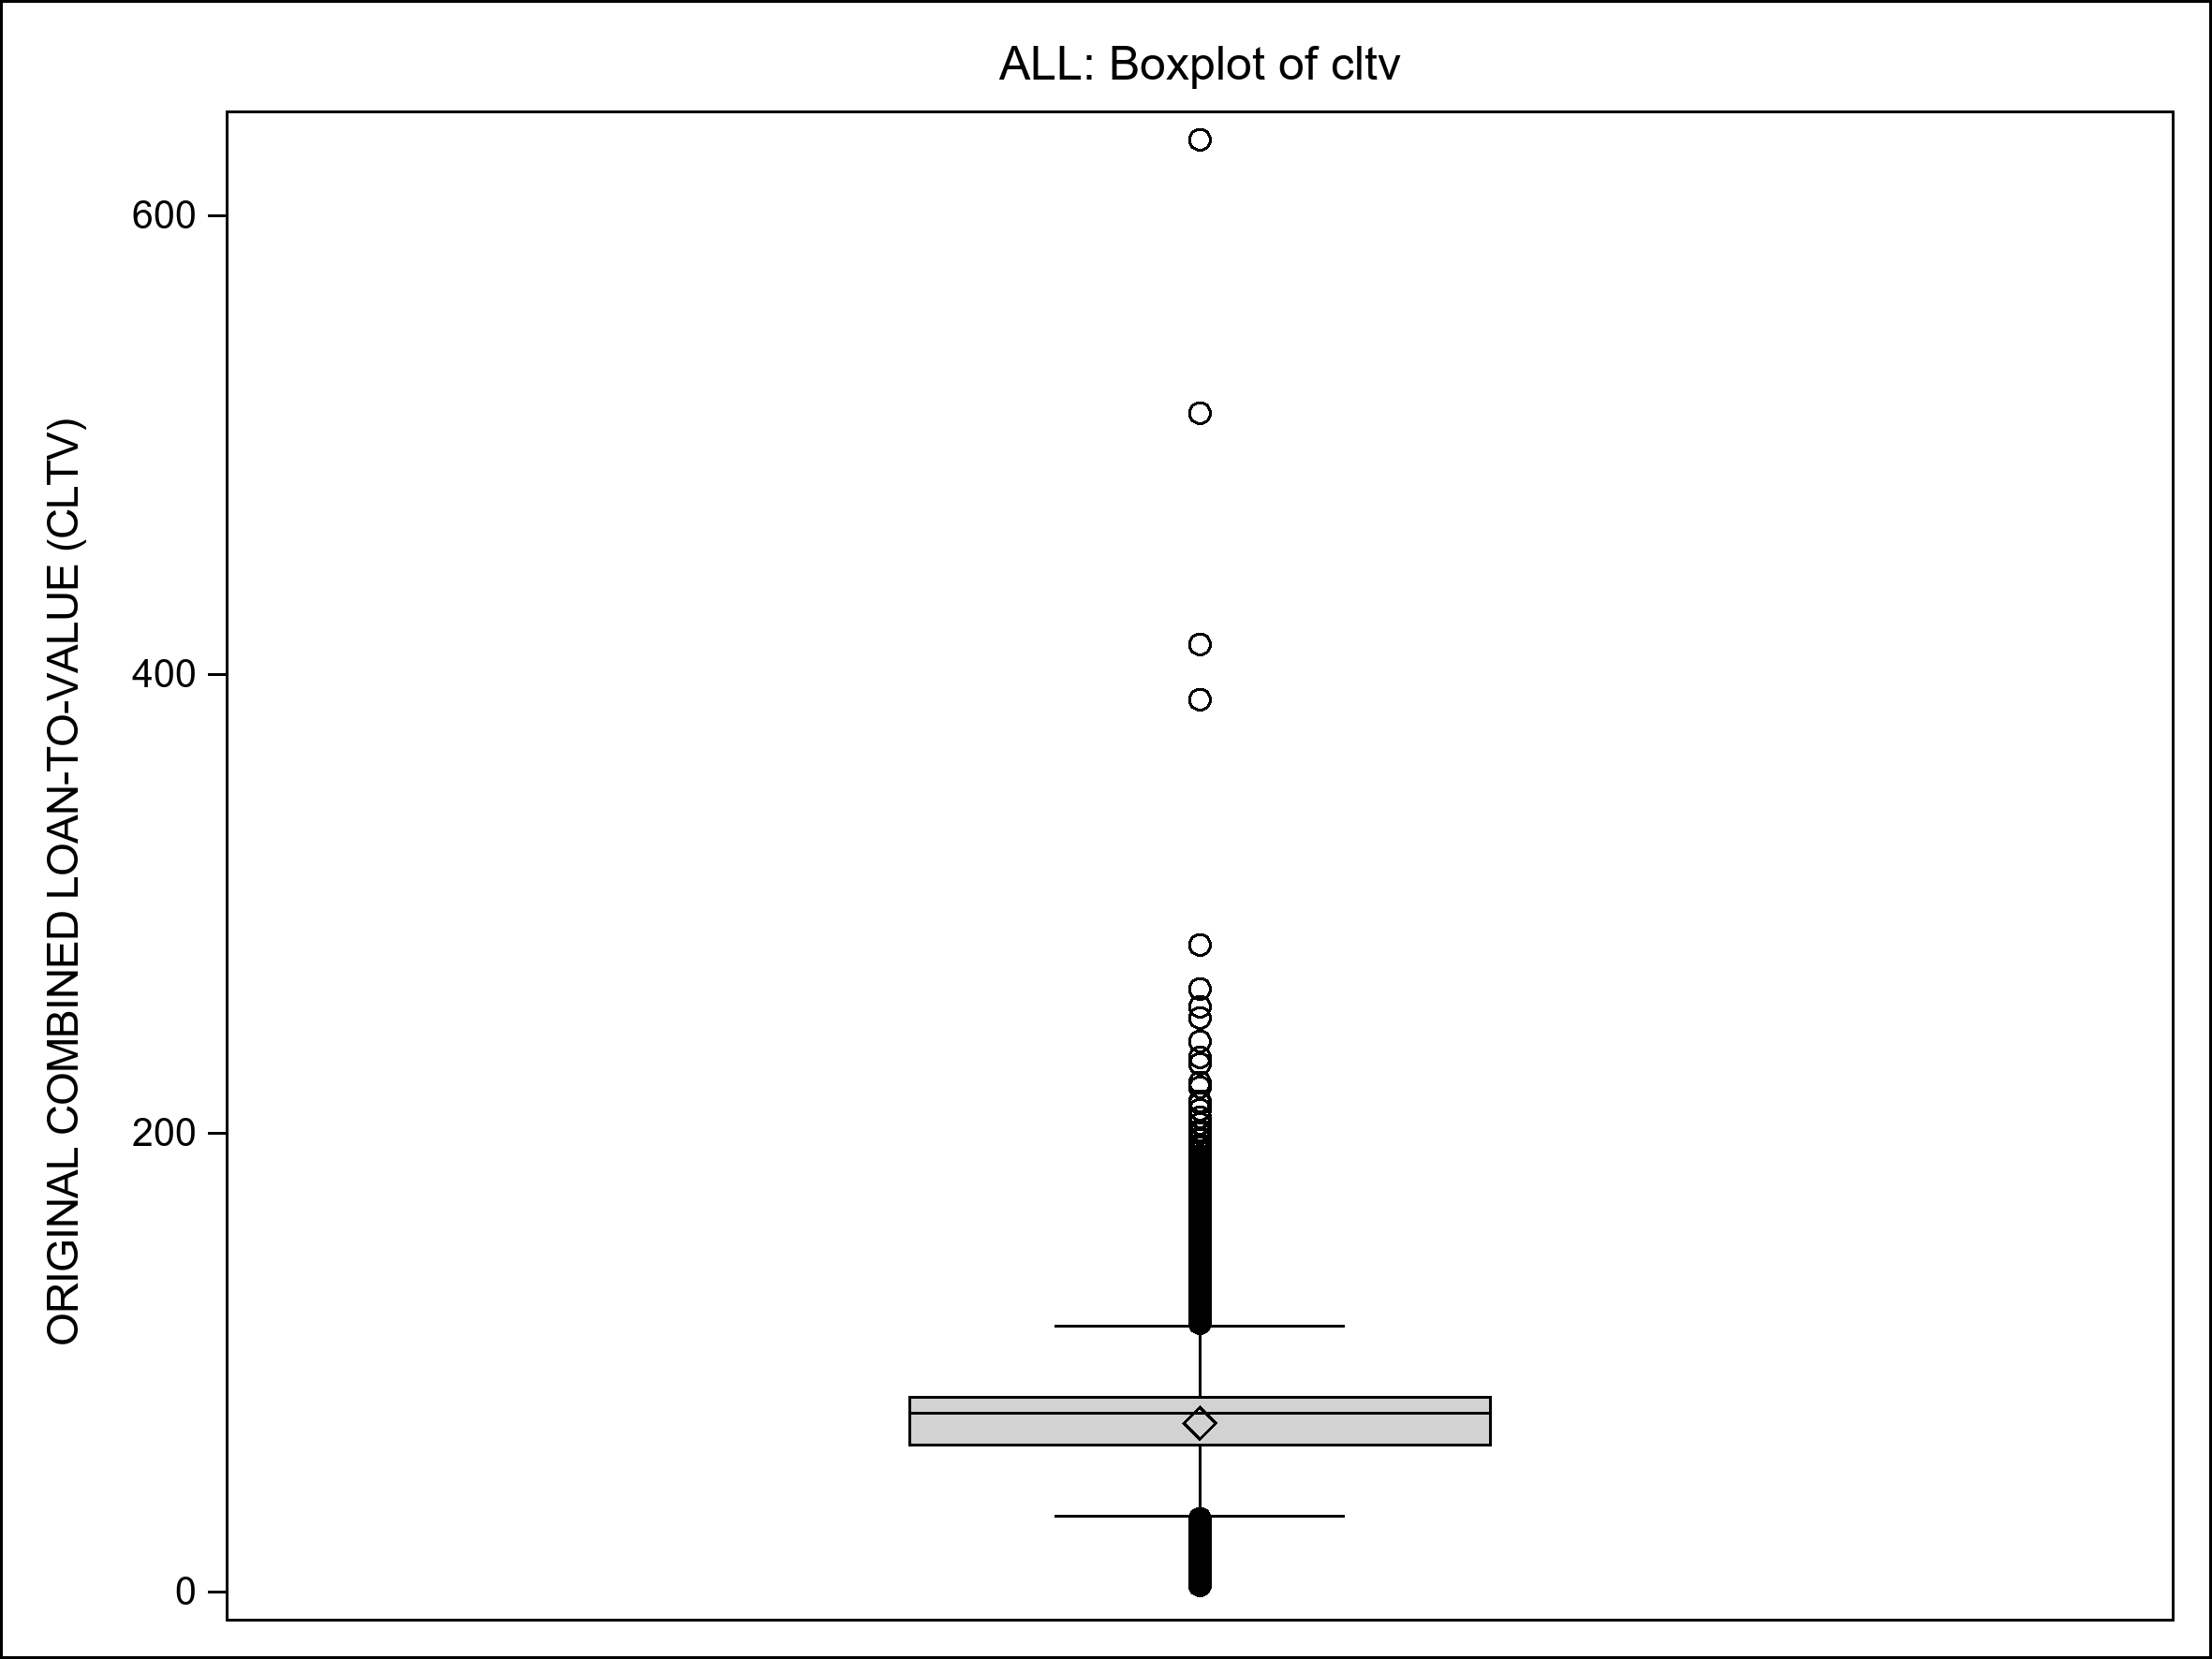
\includegraphics[width=0.9\textwidth]{./plot/Boxplot/Main/NUM_cltv_BOXPLOT_ALL1.png}
\end{minipage}%
\begin{minipage}{.5\textwidth}
	\centering
	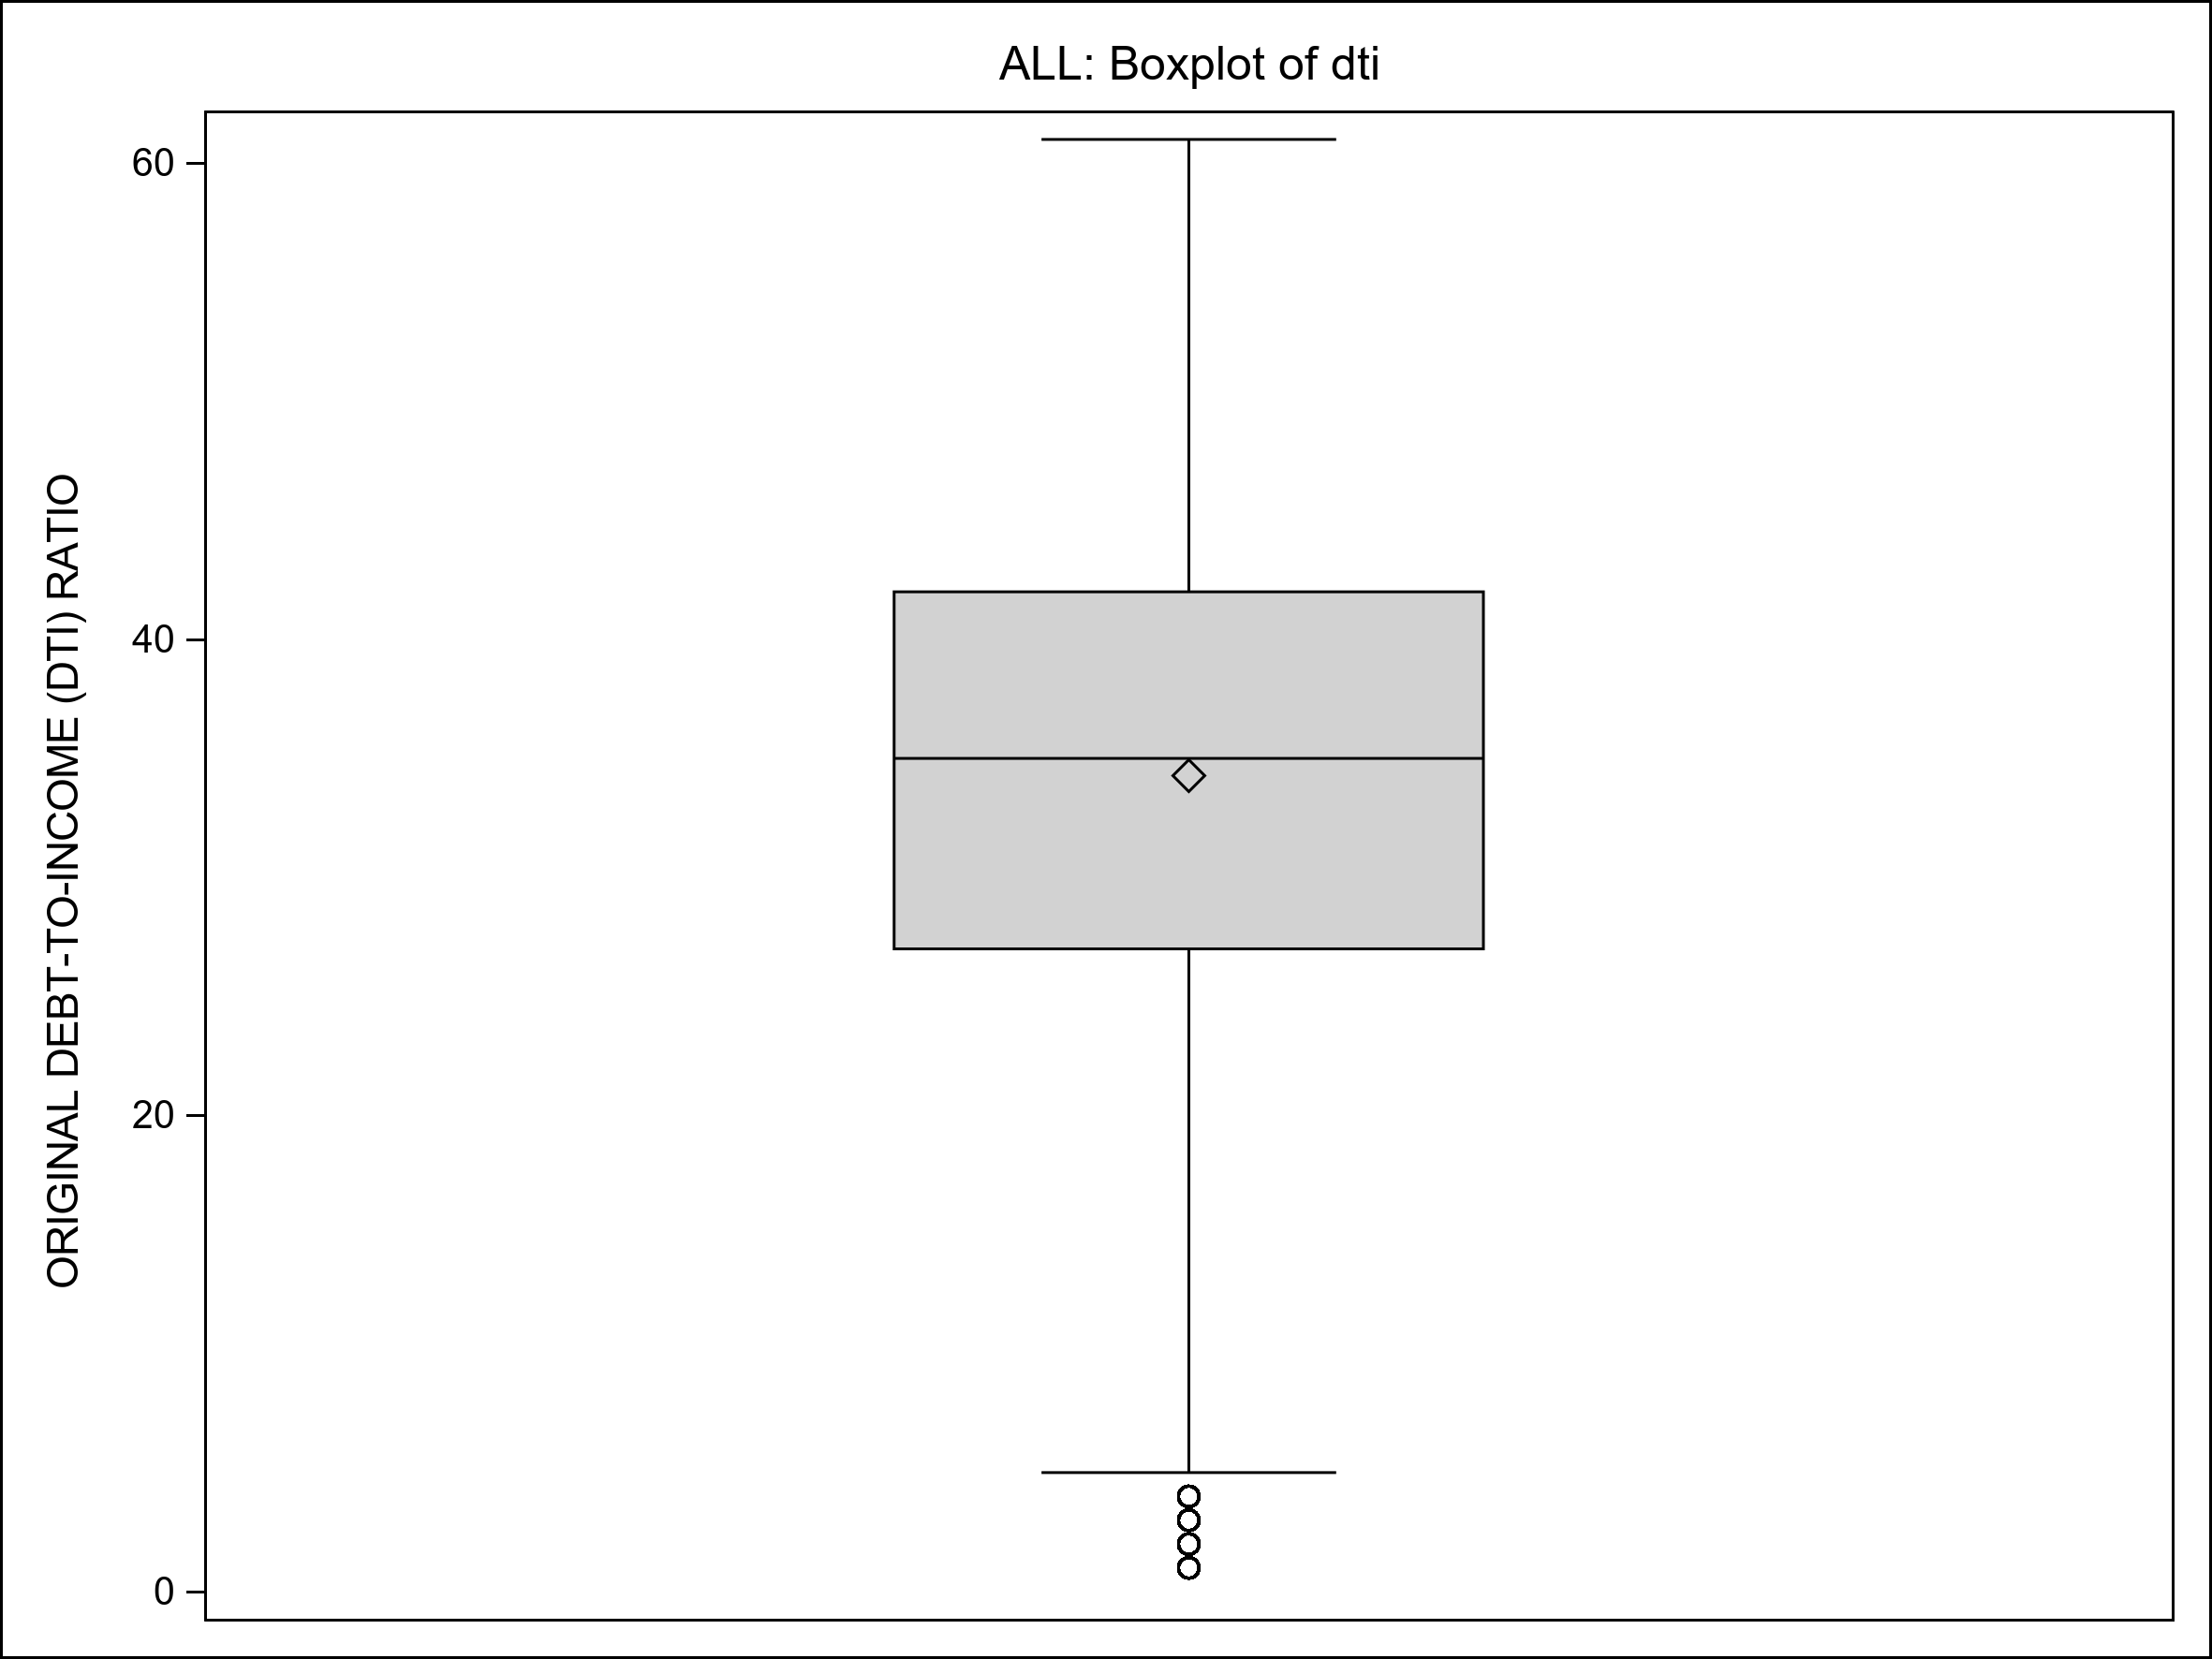
\includegraphics[width=0.9\textwidth]{./plot/Boxplot/Main/NUM_dti_BOXPLOT_ALL1.png}
\end{minipage}
    \caption{Boxplot of CLTV and DTI}
    %\label{fig:dp_iqr_boxpl}
\end{figure}
\begin{figure}[H]
\begin{minipage}{.5\textwidth}
	\centering
	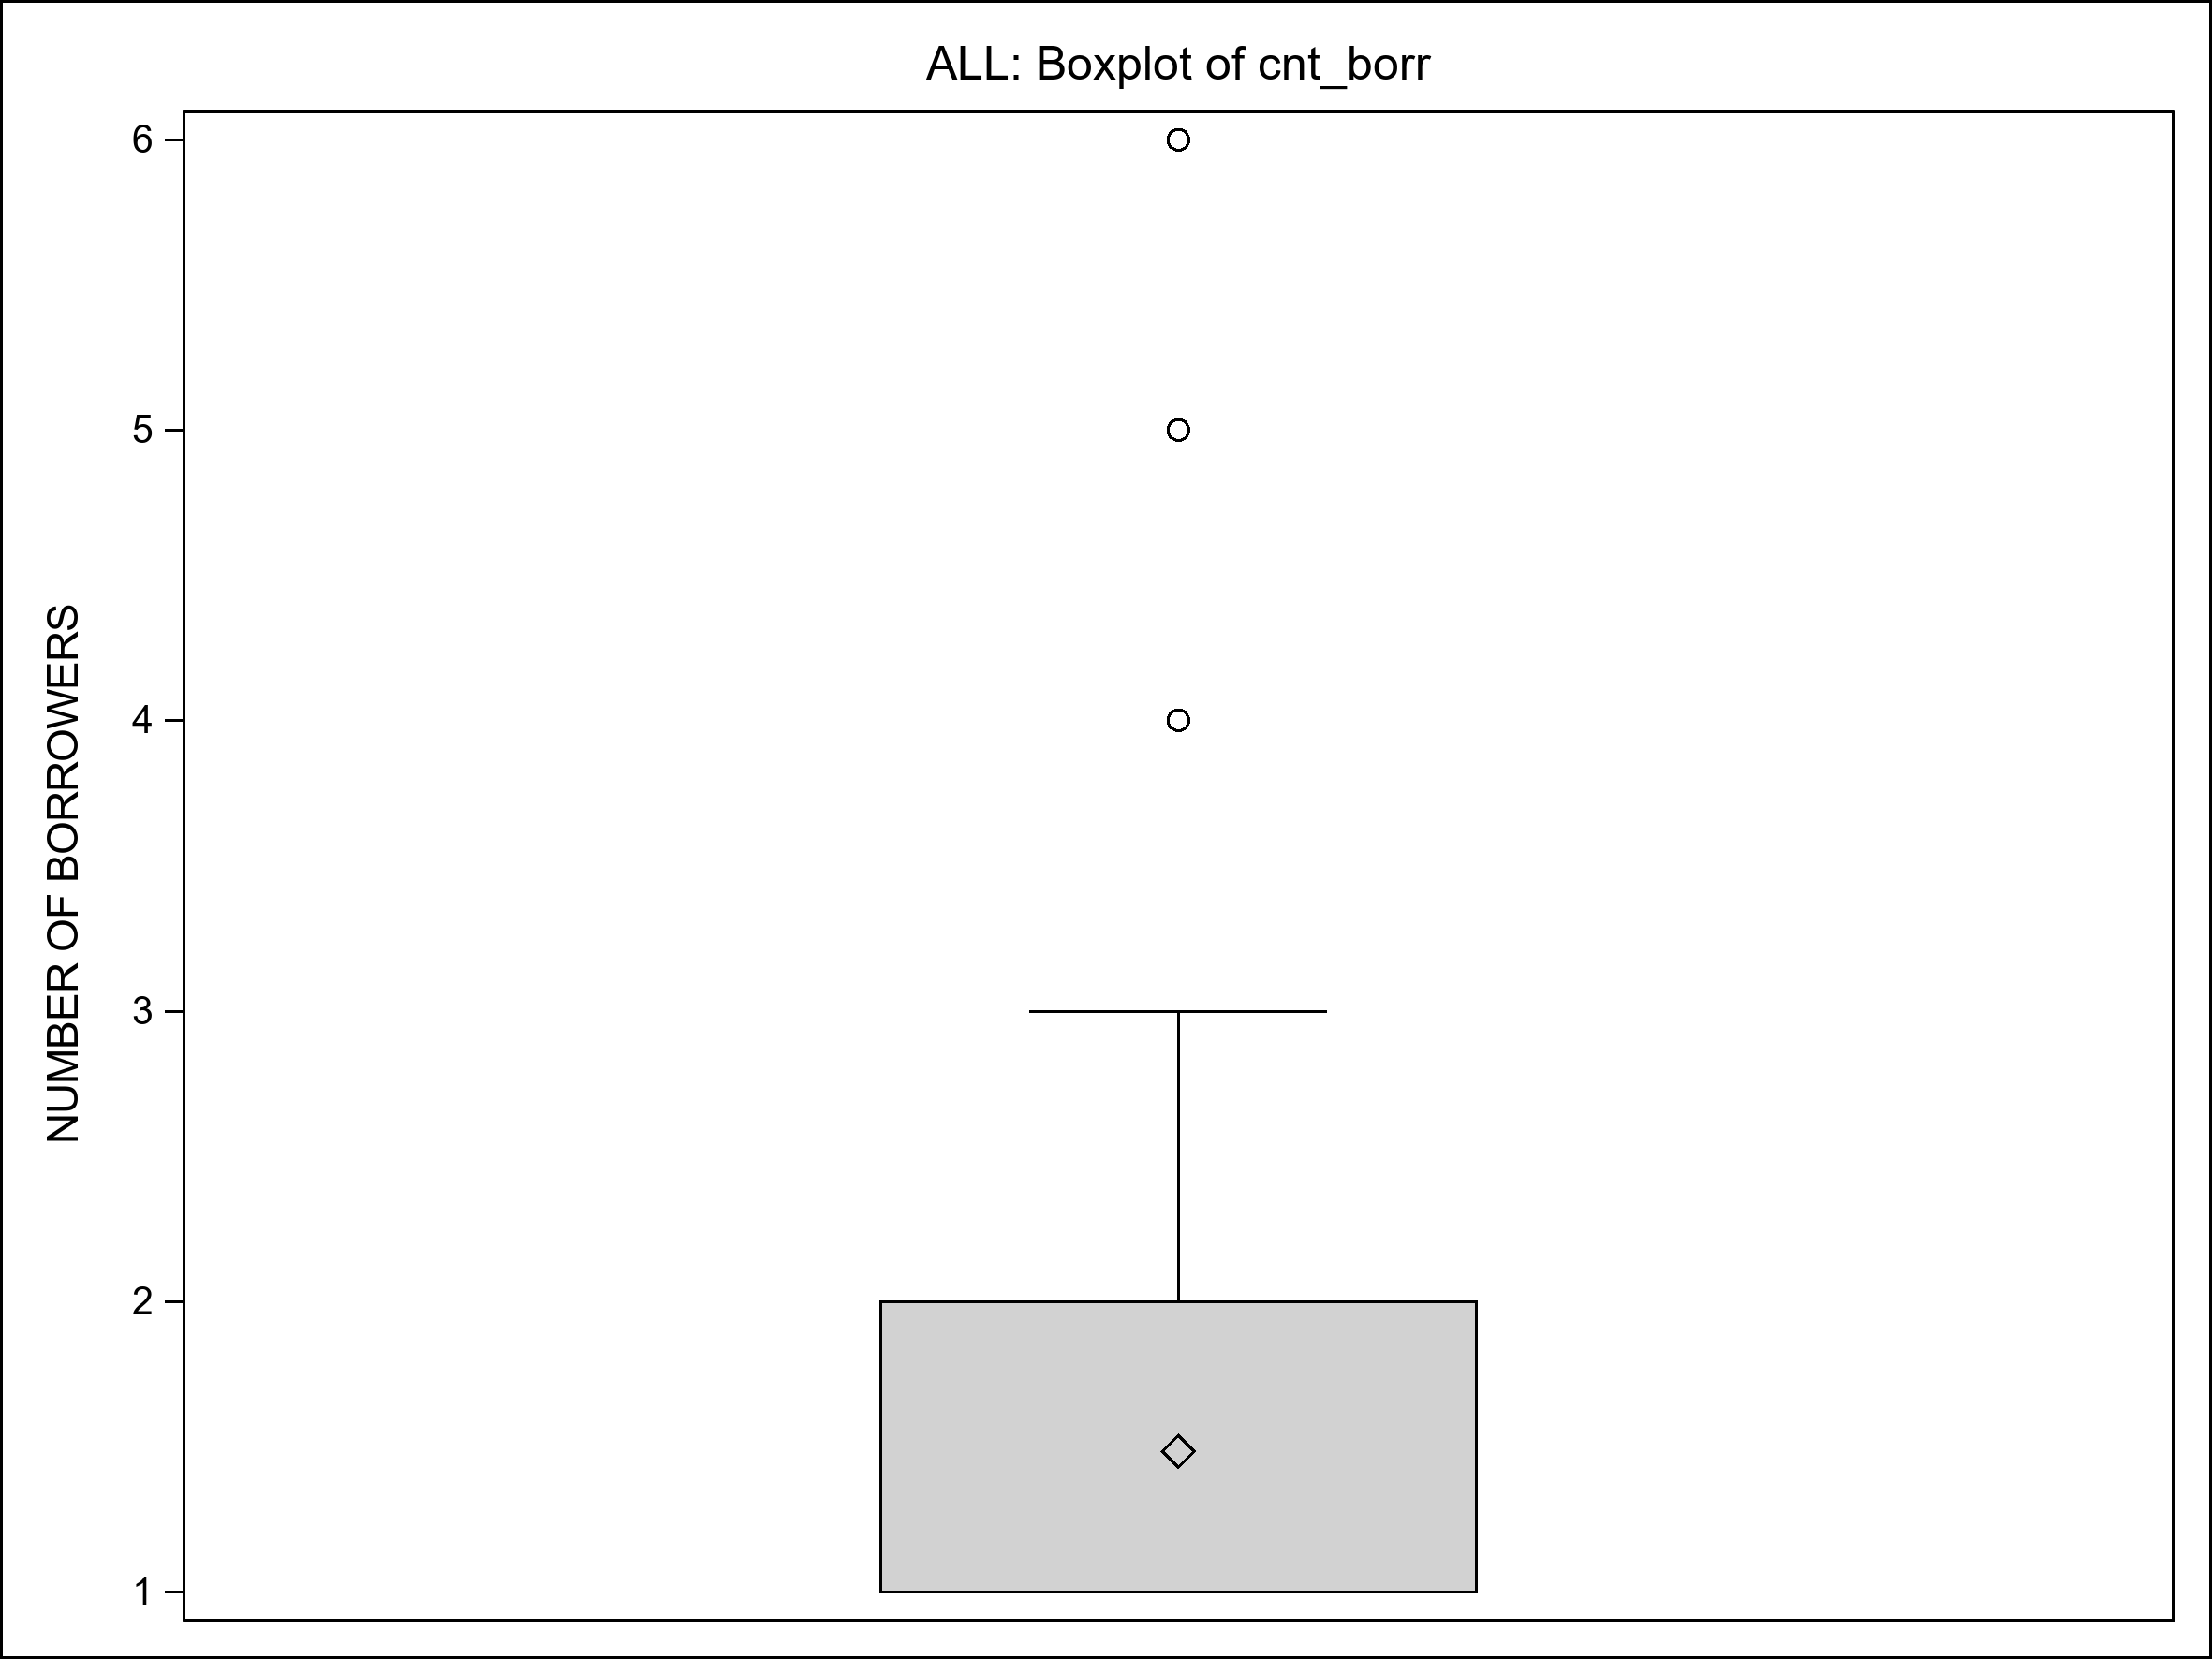
\includegraphics[width=0.9\textwidth]{./plot/Boxplot/Main/NUM_cnt_borr_BOXPLOT_ALL1.png}
\end{minipage}%
\begin{minipage}{.5\textwidth}
	\centering
	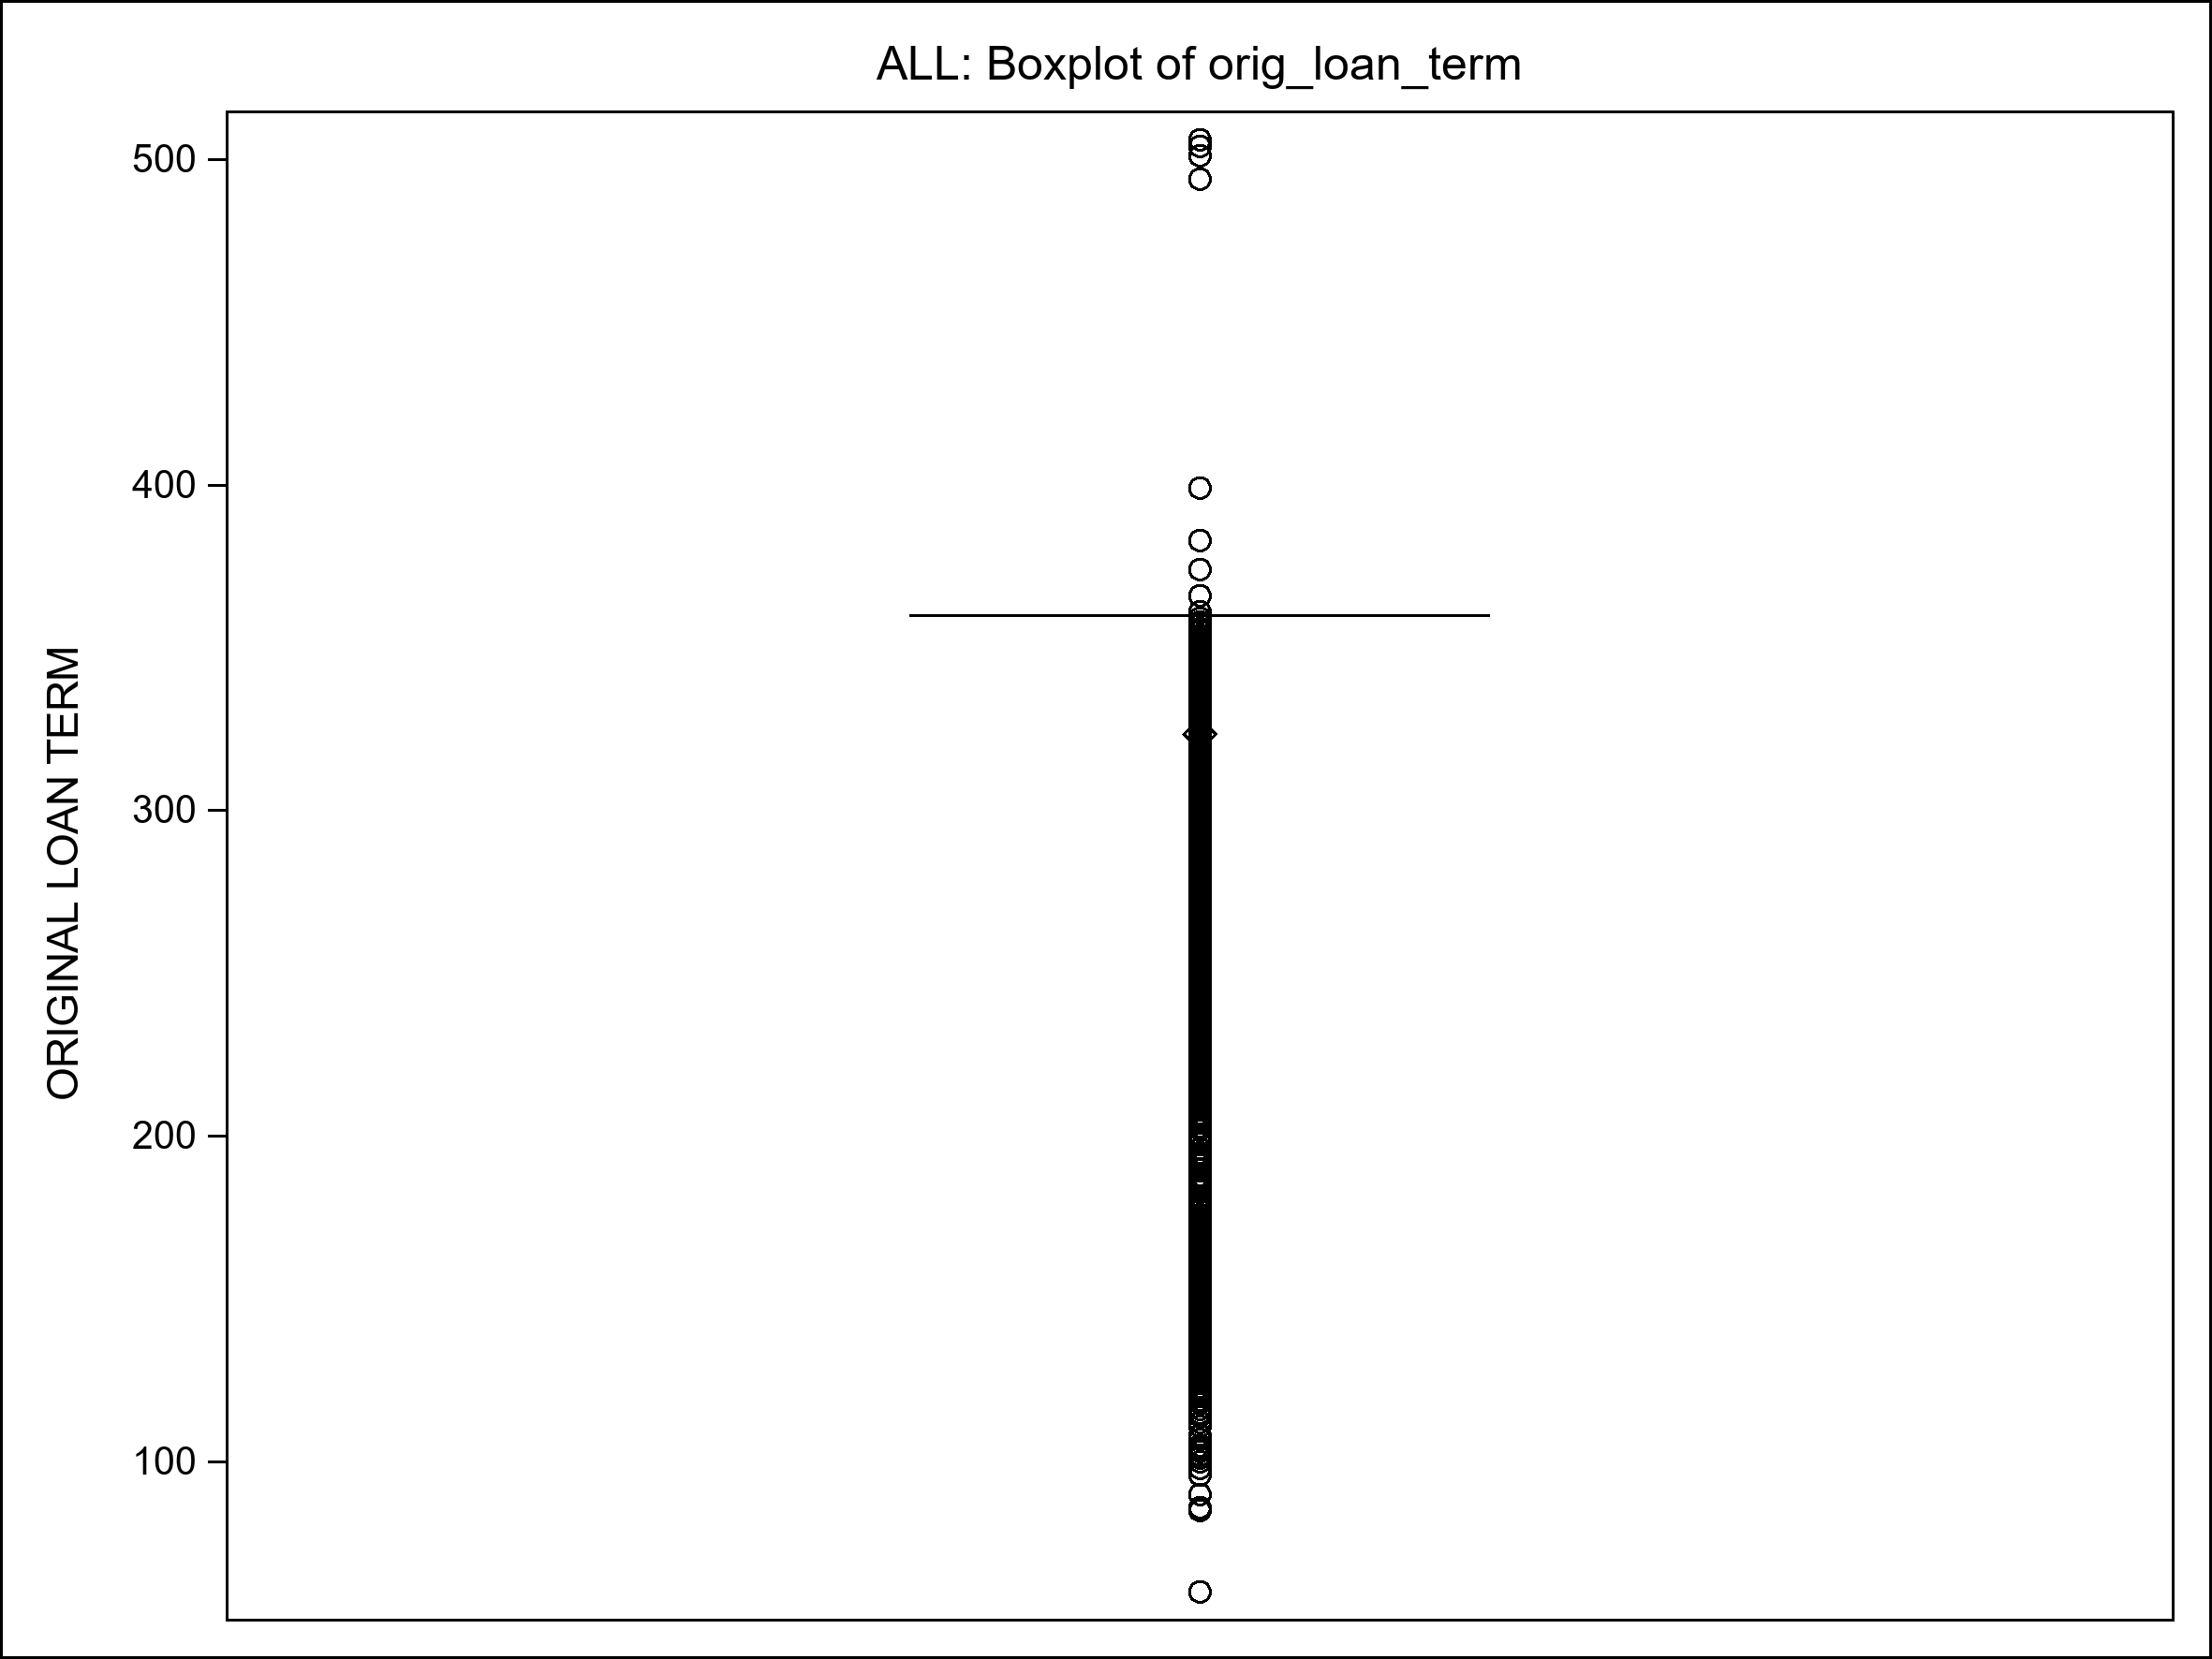
\includegraphics[width=0.9\textwidth]{./plot/Boxplot/Main/NUM_orig_loan_term_BOXPLOT_ALL1.png}
\end{minipage}
    \caption{Boxplot of Numner of Borrowers and Original Loan Term}
    \label{fig:re_boxpl_noborr_loanterm}
\end{figure}


% Please add the following required packages to your document preamble:
% \usepackage{graphicx}
% \usepackage{lscape}
\begin{landscape}

\begin{table}[]
\centering
\resizebox{1.3\textwidth}{!}{%
\begin{tabular}{llllllllllllll}\toprule
\textbf{Variable}     & \textbf{Sum}               & \textbf{Mean}    & \textbf{Mode}    & \textbf{StdDev}  & \textbf{Min}   & \textbf{P1}     & \textbf{P5}     & \textbf{P25}     & \textbf{Median}  & \textbf{P75}     & \textbf{P95}     & \textbf{P99}     & \textbf{Max}       \\\midrule
CLTV         & 398.545.357       & 73,62     & 80      & 17,27     & 3     & 25     & 39     & 64      & 78      & 85      & 95      & 97      & 633       \\
No Borrowers & 8.030.443         & 1,48      & 1       & 0,52      & 1     & 1      & 1      & 1       & 1       & 2       & 2       & 2       & 6         \\
No Units     & 5.566.001         & 1,03      & 1       & 0,22      & 1     & 1      & 1      & 1       & 1       & 1       & 1       & 2       & 4         \\
DTI          & 184.916.404       & 34,28     & 45      & 9,70      & 1     & 12     & 17     & 27      & 35      & 42      & 48      & 50      & 61        \\
Credit Score & 4.074.892.728     & 752,92    & 801     & 43,93     & 309   & 637    & 670    & 723     & 761     & 789     & 809     & 817     & 850       \\
LTV          & 397.336.584       & 73,40     & 80      & 17,29     & 3     & 24     & 39     & 64      & 77      & 85      & 95      & 97      & 514       \\
MI Perc      & 37.410.176        & 6,91      & 0       & 11,56     & 0     & 0      & 0      & 0       & 0       & 12      & 30      & 30      & 52        \\
Loan Term    & 1.751.503.811     & 323,53    & 360     & 69,96     & 60    & 180    & 180    & 360     & 360     & 360     & 360     & 360     & 506       \\
UPB          & 1.390.864.618.000 & 256916,67 & 200.000 & 131963,97 & 7.000 & 54.000 & 85.000 & 157.000 & 233.000 & 334.000 & 502.000 & 663.000 & 1.473.000 \\\bottomrule
\end{tabular}%
}
\caption{Descriptive statistics}
\label{tab:re_descr_stat}
\end{table}

\begin{table}[]
\centering
\resizebox{1.3\textwidth}{!}{%
\begin{tabular}{lrrrrrrrr}\toprule
\textbf{Variable} & \textbf{Lower Boarder}     & \textbf{Upper Boarder} & \textbf{\# below Lower Boarder} & \textbf{\# above Upper Boarder} & \textbf{\% below Lower Boarder} & \textbf{\% above Upper Boarder} & \textbf{\# Outliers} & \textbf{\% Outliers} \\\midrule
CLTV         & 32,5    & 116,5  & 142518  & 596    & 2,63\%  & 0,01\% & 143.114   & 2,64\%  \\
No Borrowers & -0,5    & 3,5    & 0       & 5461   & 0,00\%  & 0,10\% & 5.461     & 0,10\%  \\
No Units     & 1       & 1      & 0       & 108940 & 0,00\%  & 2,01\% & 108.940   & 2,01\%  \\
DTI          & 4,5     & 64,5   & 21294   & 0      & 0,39\%  & 0,00\% & 21.294    & 0,39\%  \\
Credit Score & 624     & 888    & 16444   & 0      & 0,30\%  & 0,00\% & 16.444    & 0,30\%  \\
LTV          & 32,5    & 116,5  & 145323  & 394    & 2,68\%  & 0,01\% & 145.717   & 2,69\%  \\
MI Perc      & -18     & 30     & 19      & 25853  & 0,00\%  & 0,48\% & 25.872    & 0,48\%  \\
Loan Term    & 360     & 360    & 1236041 & 18     & 22,83\% & 0,00\% & 1.236.059 & 22,83\% \\
UPB          & -108500 & 599500 & 0       & 102141 & 0,00\%  & 1,89\% & 102.141   & 1,89\%   \\\bottomrule                                
\end{tabular}%
}
\caption{Interquartile range}
\label{tab:re_iqr}
\end{table}

\end{landscape}

\section{Variable Selection}
\subsection{Univariate Analysis}

\subsubsection{New variables}
During the outlier treatment, a few new variables were created. While analyzing the different distinct values of categorical variables, the risk factor \emph{Property states} were grouped into five \emph{US regions} according to their geographical position: Northeast, Southeast, Southwest, Midwest, West and other Regions, e.g., outside of the North American mainland.\footnote{\cite{USRegion:2014}} Table \ref{tab:re_descr_newvar} lists a summary of the new variables.

\begin{table}[H]
\centering
\begin{tabular}{ Lp{8cm}R } \toprule
\textbf{Variable Name}  & \textbf{Description}                                                                                                                                                                                                                                                          & \textbf{Abbr.}       \\\midrule
MI Percentage Indicator                                        & Indicator, that Mortgage Insurance Percentage \textgreater 0\%                           & MI Flag                     \\\hline
Loan Term \textgreater 360 Months                              & Indicator, that Original Loan Term \textgreater 360 Months                               & Loan Term \textgreater 360m \\\hline
Loan Term Group                                                & Grouped Variable, Original Loan Term is "\textless 360m", "= 360m", "\textgreater{}360m" & Loan Term Group             \\\hline
Loan Term $\geq$ 360 Months Indicator                          & Indicator, that Original Loan Term $\geq$ 360 Months                                     & Loan Term $\geq$ 360m        \\\hline
Indicator, that Original Loan Term = 360 Months                & Indicator, that Original Loan Term = 360 Months                                          & Loan Term = 360m            \\\hline
Original Combined Loan-to-Value (CLTV) after Outlier Treatment & Original Combined Loan-to-Value (CLTV) after Outlier Treatment                           & CLTV adj                    \\\hline
Original Loan-to-Value (LTV) after Outlier Treatment           & Original Loan-to-Value (LTV) after Outlier Treatment                                     & LTV adj                     \\\hline
US Region                                                      & Grouped variable of "Property State"                                                     & US Region                \\\bottomrule
\end{tabular}%
\caption{Description of new variables}
\label{tab:re_descr_newvar}
\end{table}

\subsubsection{Discriminatory Power}
To assess the discriminatory power, distribution plots with default rates, ROC curves and calculations of AUC, Gini coefficients, WoE and IV were conducted. A list of all metrics is presented in Table \ref{tab:re_discr_power} and relevant variable plots are depicted in Figures \ref{fig:re_fico_upb} to \ref{fig:re_usreg_channel}. All plots are available in Appendix \ref{sec:distr_all} and \ref{sec:ROC_all}. As expected, the external \emph{Credit Score} provided by FICO shows the highest discriminatory power, followed by financial ratios such as \emph{DTI}, \emph{LTV} and \emph{CLTV}. Other numerical risk factors, except \emph{No Units}, also indicate good predictive power, making them optimal candidates for the modeling process. In contrast,  the performance of categorical and indicator risk factors proved underwhelming, with few Gini coefficients surpassing 5\% or IV exceeding 3\%. Consequently, a Gini threshold of 5\% and IV of 3\% was established for the selection process of the long list.

To summarize, all variables with a missing proportion below 20\%, outlier proportion not succeeding 20\%, Gini coefficient above 5\% and IV higher than 3\% were selected for the long list given in Tab. \ref{tab:re_ll_sl}. 

{
\footnotesize

\begin{longtable}{ p{3cm} p{4cm} c c c c c}\toprule      
\textbf{Variable}           & \textbf{Value}                                     & \textbf{\% Missing} & \textbf{AUC}    & \textbf{Gini}  & \textbf{WoE} & \textbf{IV}  \\\midrule
Amort Type                  & Fixed Rate Mortgage                                               & 0,00\%  & 0,5000 & 0,0000 & 0,0000  & 0,0000 \\\hline
Prop Val Method             & ACE Loans                                                         & 0,07\%  & 0,5402 & 0,0805 & 0,4326  & 0,0486 \\
                            & Full Appraisal                                                    & 0,07\%  & 0,5445 & 0,0890 & -0,1126 & 0,0486 \\
                            & Other Appraisals (Desktop, driveby, external, AVM)                & 0,07\%  & 0,5042 & 0,0084 & 0,4429  & 0,0486 \\
                            & Not Available                                                     & 0,07\%  & 0,5001 & 0,0001 & 0,2385  & 0,0486 \\\hline
Channel                     & Not Available                                                     & 0,00\%  & 0,5000 & 0,0000 & 0,0000  & 0,0358 \\
                            & Broker                                                            & 0,00\%  & 0,5047 & 0,0095 & -0,0811 & 0,0358 \\
                            & Correspondent                                                     & 0,00\%  & 0,5411 & 0,0822 & -0,2318 & 0,0358 \\
                            & Retail                                                            & 0,00\%  & 0,5458 & 0,0917 & 0,1744  & 0,0358 \\\hline
Prog Flag                   & Not Available or Not Applicable                                   & 92,48\% & 0,5178 & 0,0355 & 0,0391  & 0,0176 \\
                            & HFA Advantage                                                     & 92,48\% & 0,5039 & 0,0078 & -0,8763 & 0,0176 \\
                            & Home Possible                                                     & 92,48\% & 0,5138 & 0,0277 & -0,3369 & 0,0176 \\\hline
Loan Purpose                & Refinance - Cash Out               								& 0,00\%  & 0,5144 & 0,0289 & -0,1380 & 0,0080 \\
                            & Refinance - No Cash Out 											& 0,00\%  & 0,5179 & 0,0358 & 0,1096  & 0,0080 \\
                            & Purchase                                                          & 0,00\%  & 0,5035 & 0,0069 & -0,0149 & 0,0080 \\\hline
Occupancy                   & Investment Property                                               & 0,00\%  & 0,5027 & 0,0053 & -0,0838 & 0,0055 \\
                            & Primary Residence                                                 & 0,00\%  & 0,5037 & 0,0074 & -0,0082 & 0,0055 \\
                            & Second Home                                                       & 0,00\%  & 0,5063 & 0,0127 & 0,3945  & 0,0055 \\\hline
Loan Term Group             & = 360 Months                                                      & 0,00\%  & 0,5473 & 0,0946 & -0,1158 & 0,0615 \\
                            & \textgreater{} 360 Months                                         & 0,00\%  & 0,5000 & 0,0001 & -3,4796 & 0,0615 \\
                            & \textless{} 360 Months                                            & 0,00\%  & 0,5473 & 0,0947 & 0,5310  & 0,0615 \\\hline
Prop Type                   & Condo                                                             & 0,00\%  & 0,5024 & 0,0048 & -0,0582 & 0,0005 \\
                            & Co-op                                                             & 0,00\%  & 0,5002 & 0,0003 & 0,2712  & 0,0005 \\
                            & Manufactured Housing    											& 0,00\%  & 0,5003 & 0,0005 & 0,1516  & 0,0005 \\
                            & PUD                                                               & 0,00\%  & 0,5010 & 0,0020 & -0,0073 & 0,0005 \\
                            & Single-Family                                                     & 0,00\%  & 0,5029 & 0,0059 & 0,0093  & 0,0005 \\\hline
US Region                   & Midwest                                                           & 0,00\%  & 0,5317 & 0,0634 & 0,3194  & 0,0300 \\
                            & Northeast                                                         & 0,00\%  & 0,5151 & 0,0301 & -0,2016 & 0,0300 \\
                            & Other                                                             & 0,00\%  & 0,5002 & 0,0004 & -0,7108 & 0,0300 \\
                            & South                                                             & 0,00\%  & 0,5004 & 0,0009 & -0,0025 & 0,0300 \\
                            & West                                                              & 0,00\%  & 0,5160 & 0,0320 & -0,1064 & 0,0300 \\\hline
Homebuyer Flag              &                                                                   & 0,00\%  & 0,5167 & 0,0333 & 0,0000  & 0,0068 \\
Int Only Flag               &                                                                   & 0,00\%  & 0,5000 & 0,0000 & 0,0000  & 0,0000 \\
MI Flag                     &                                                                   & 0,00\%  & 0,5531 & 0,1062 & 0,0000  & 0,0510 \\
Loan Term = 360m            &                                                                   & 0,00\%  & 0,5473 & 0,0946 & 0,0000  & 0,0611 \\
Loan Term $\geq$ 360m       &                                                                   & 0,00\%  & 0,5473 & 0,0947 & 0,0000  & 0,0612 \\
Loan Term \textgreater 360m &                                                                   & 0,00\%  & 0,5000 & 0,0001 & 0,0000  & 0,0002 \\
Sup Conf Flag               &                                                                   & 96,51\% & 0,5000 & 0,0000 & 0,0000  & 0,0158 \\
HARP Flag                   &                                                                   & 99,66\% & 0,5000 & 0,0000 & 0,0000  & 0,0013 \\
PPM Flag                    &                                                                   & 0,00\%  & 0,5000 & 0,0000 & 0,0000  & 0,0000 \\\hline
CLTV                        &                                                                   & 0,00\%  & 0,5872 & 0,1744 & 0,0000  & 0,1087 \\
No Borrowers                &                                                                   & 0,00\%  & 0,5504 & 0,1007 & 0,0000  & 0,0537 \\
No Units                    &                                                                   & 0,00\%  & 0,5078 & 0,0156 & 0,0000  & 0,0092 \\
DTI                         &                                                                   & 0,35\%  & 0,6354 & 0,2709 & 0,0000  & 0,2709 \\
Credit Score                &                                                                   & 0,03\%  & 0,6647 & 0,3294 & 0,0000  & 0,3467 \\
LTV                         &                                                                   & 0,00\%  & 0,5854 & 0,1708 & 0,0000  & 0,1051 \\
MI Perc                     &                                                                   & 0,00\%  & 0,5546 & 0,1091 & 0,0000  & 0,0543 \\
Loan Term                   &                                                                   & 0,00\%  & 0,5487 & 0,0974 & 0,0000  & 0,0661 \\
UPB                         &                                                                   & 0,00\%  & 0,5792 & 0,1583 & 0,0000  & 0,0778 \\\bottomrule
    
\caption{Discriminatory power}
\label{tab:re_discr_power}           
\end{longtable}
}

\begin{figure}[H]
\begin{minipage}{.5\textwidth}
	\centering
	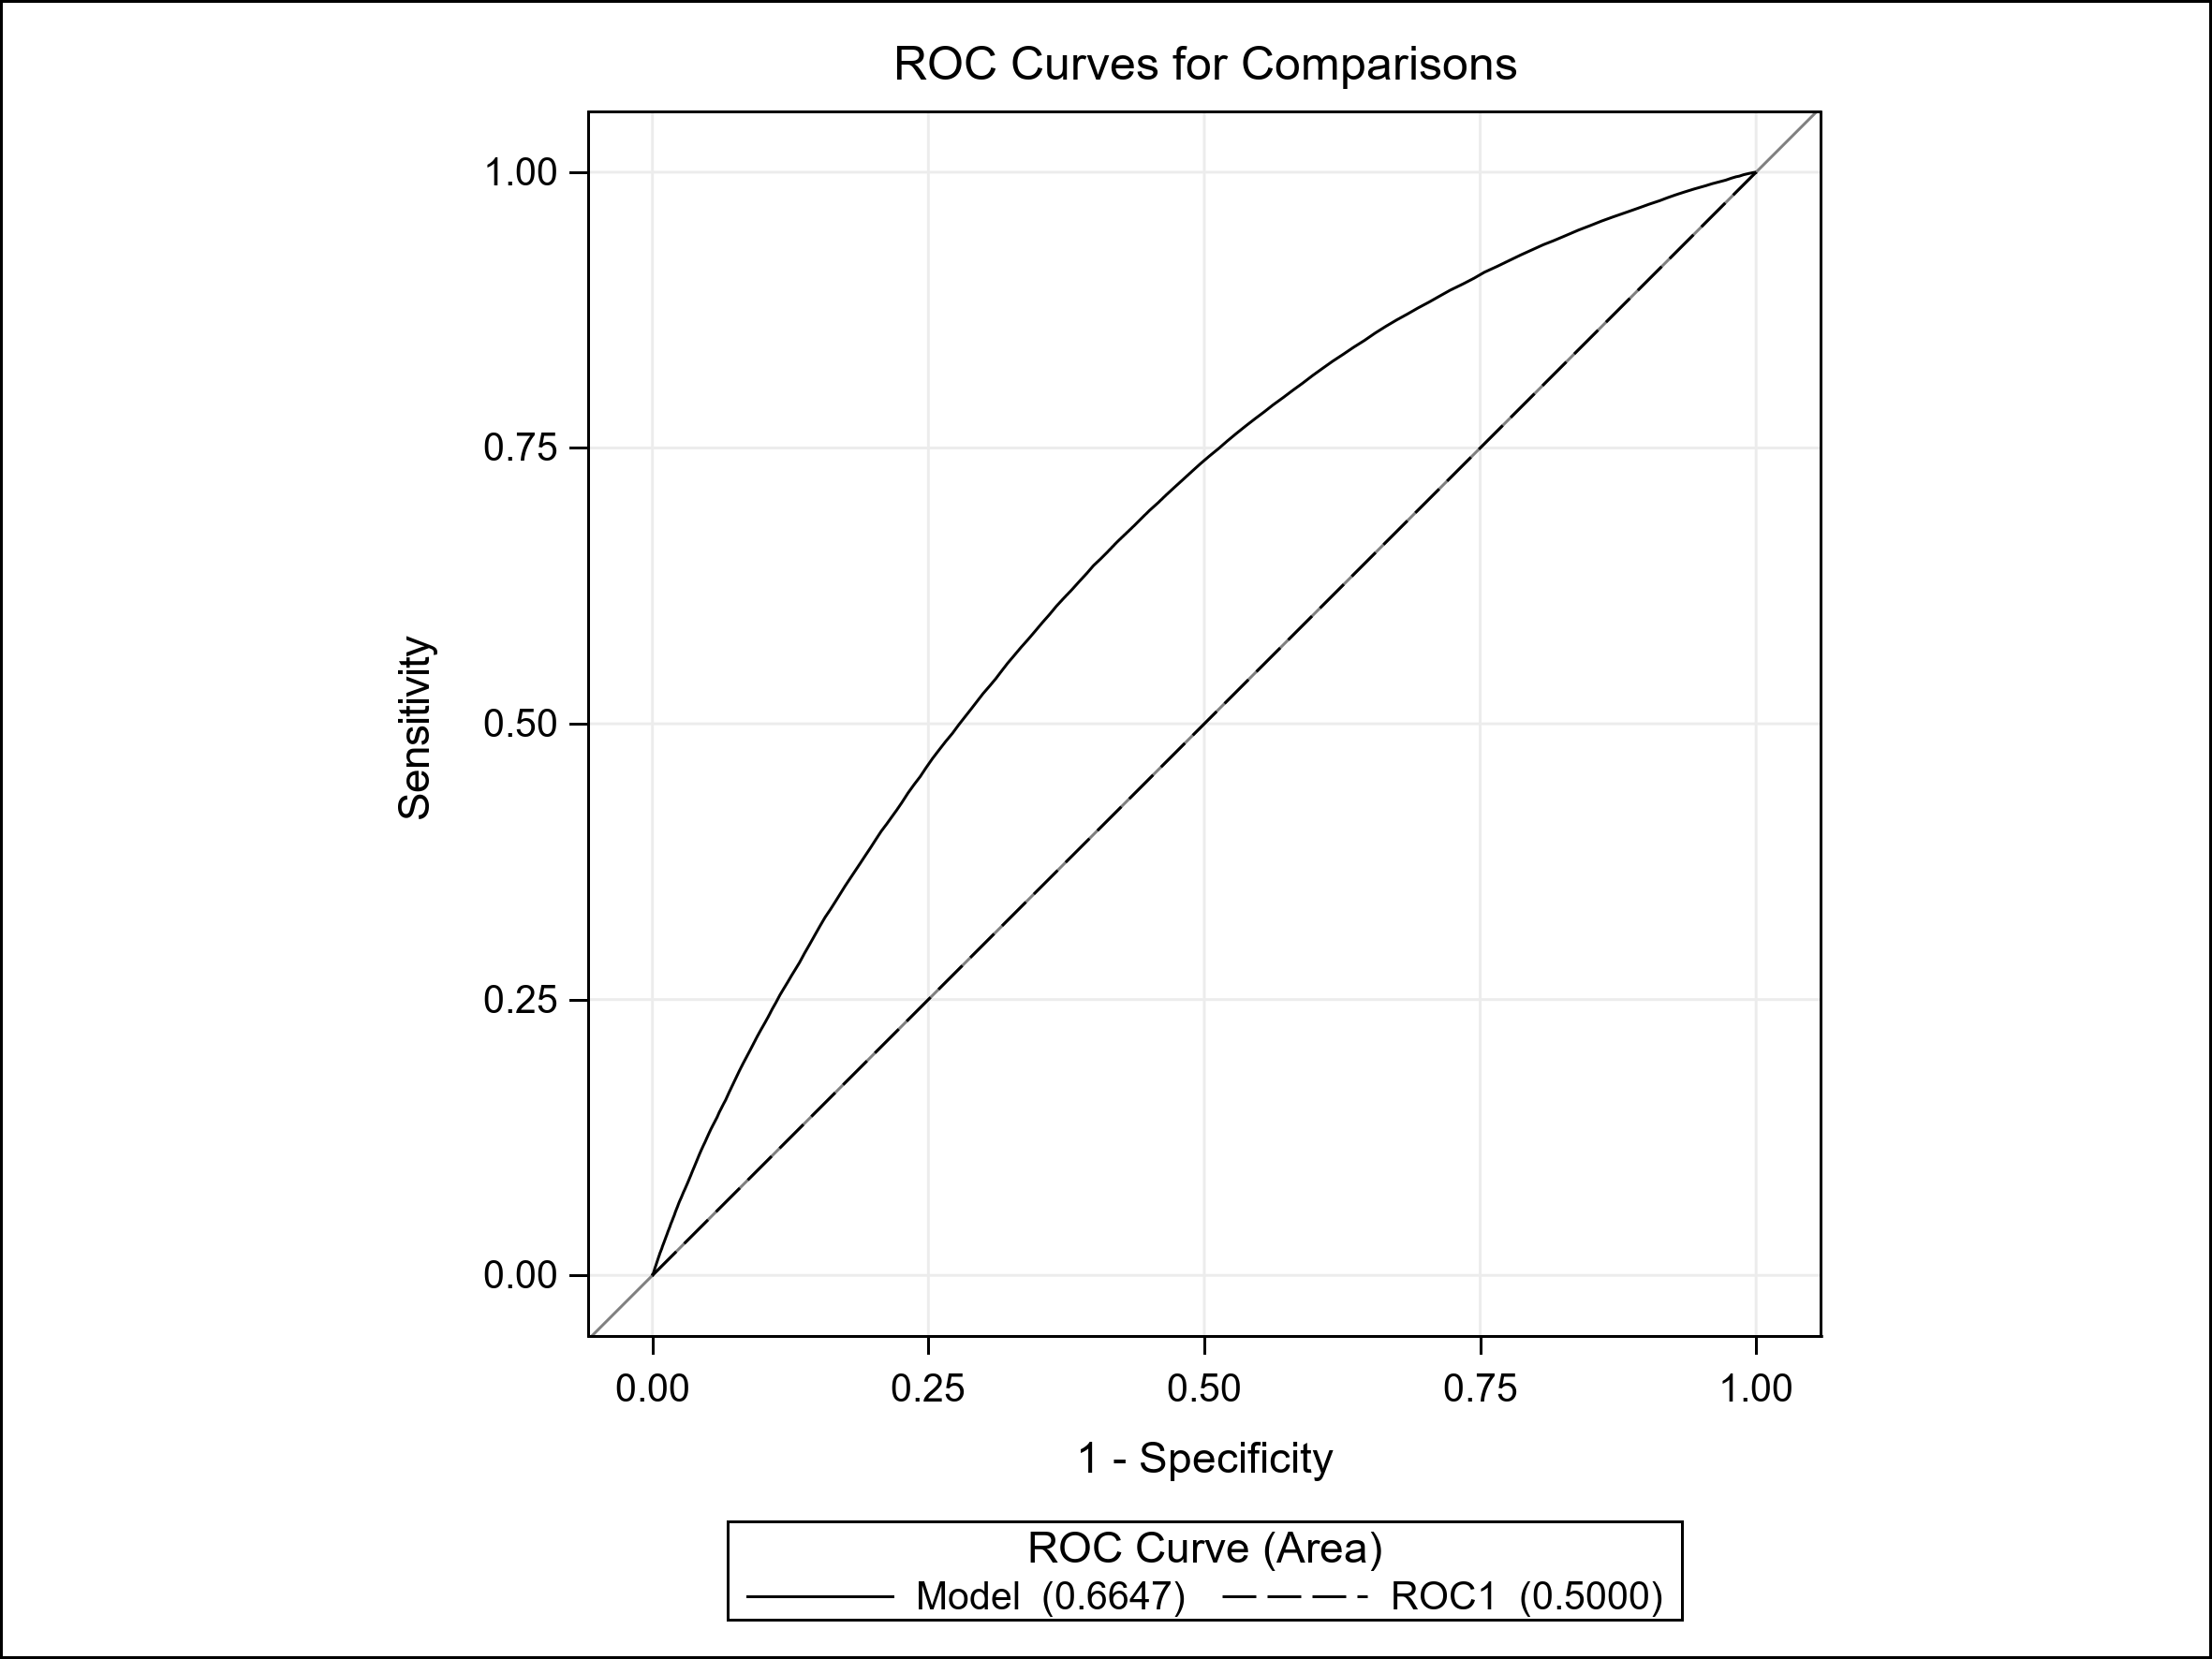
\includegraphics[width=0.9\textwidth]{./plot/ROC/Main/NUM_fico_ROC_ALL5.png}
\end{minipage}%
\begin{minipage}{.5\textwidth}
	\centering
	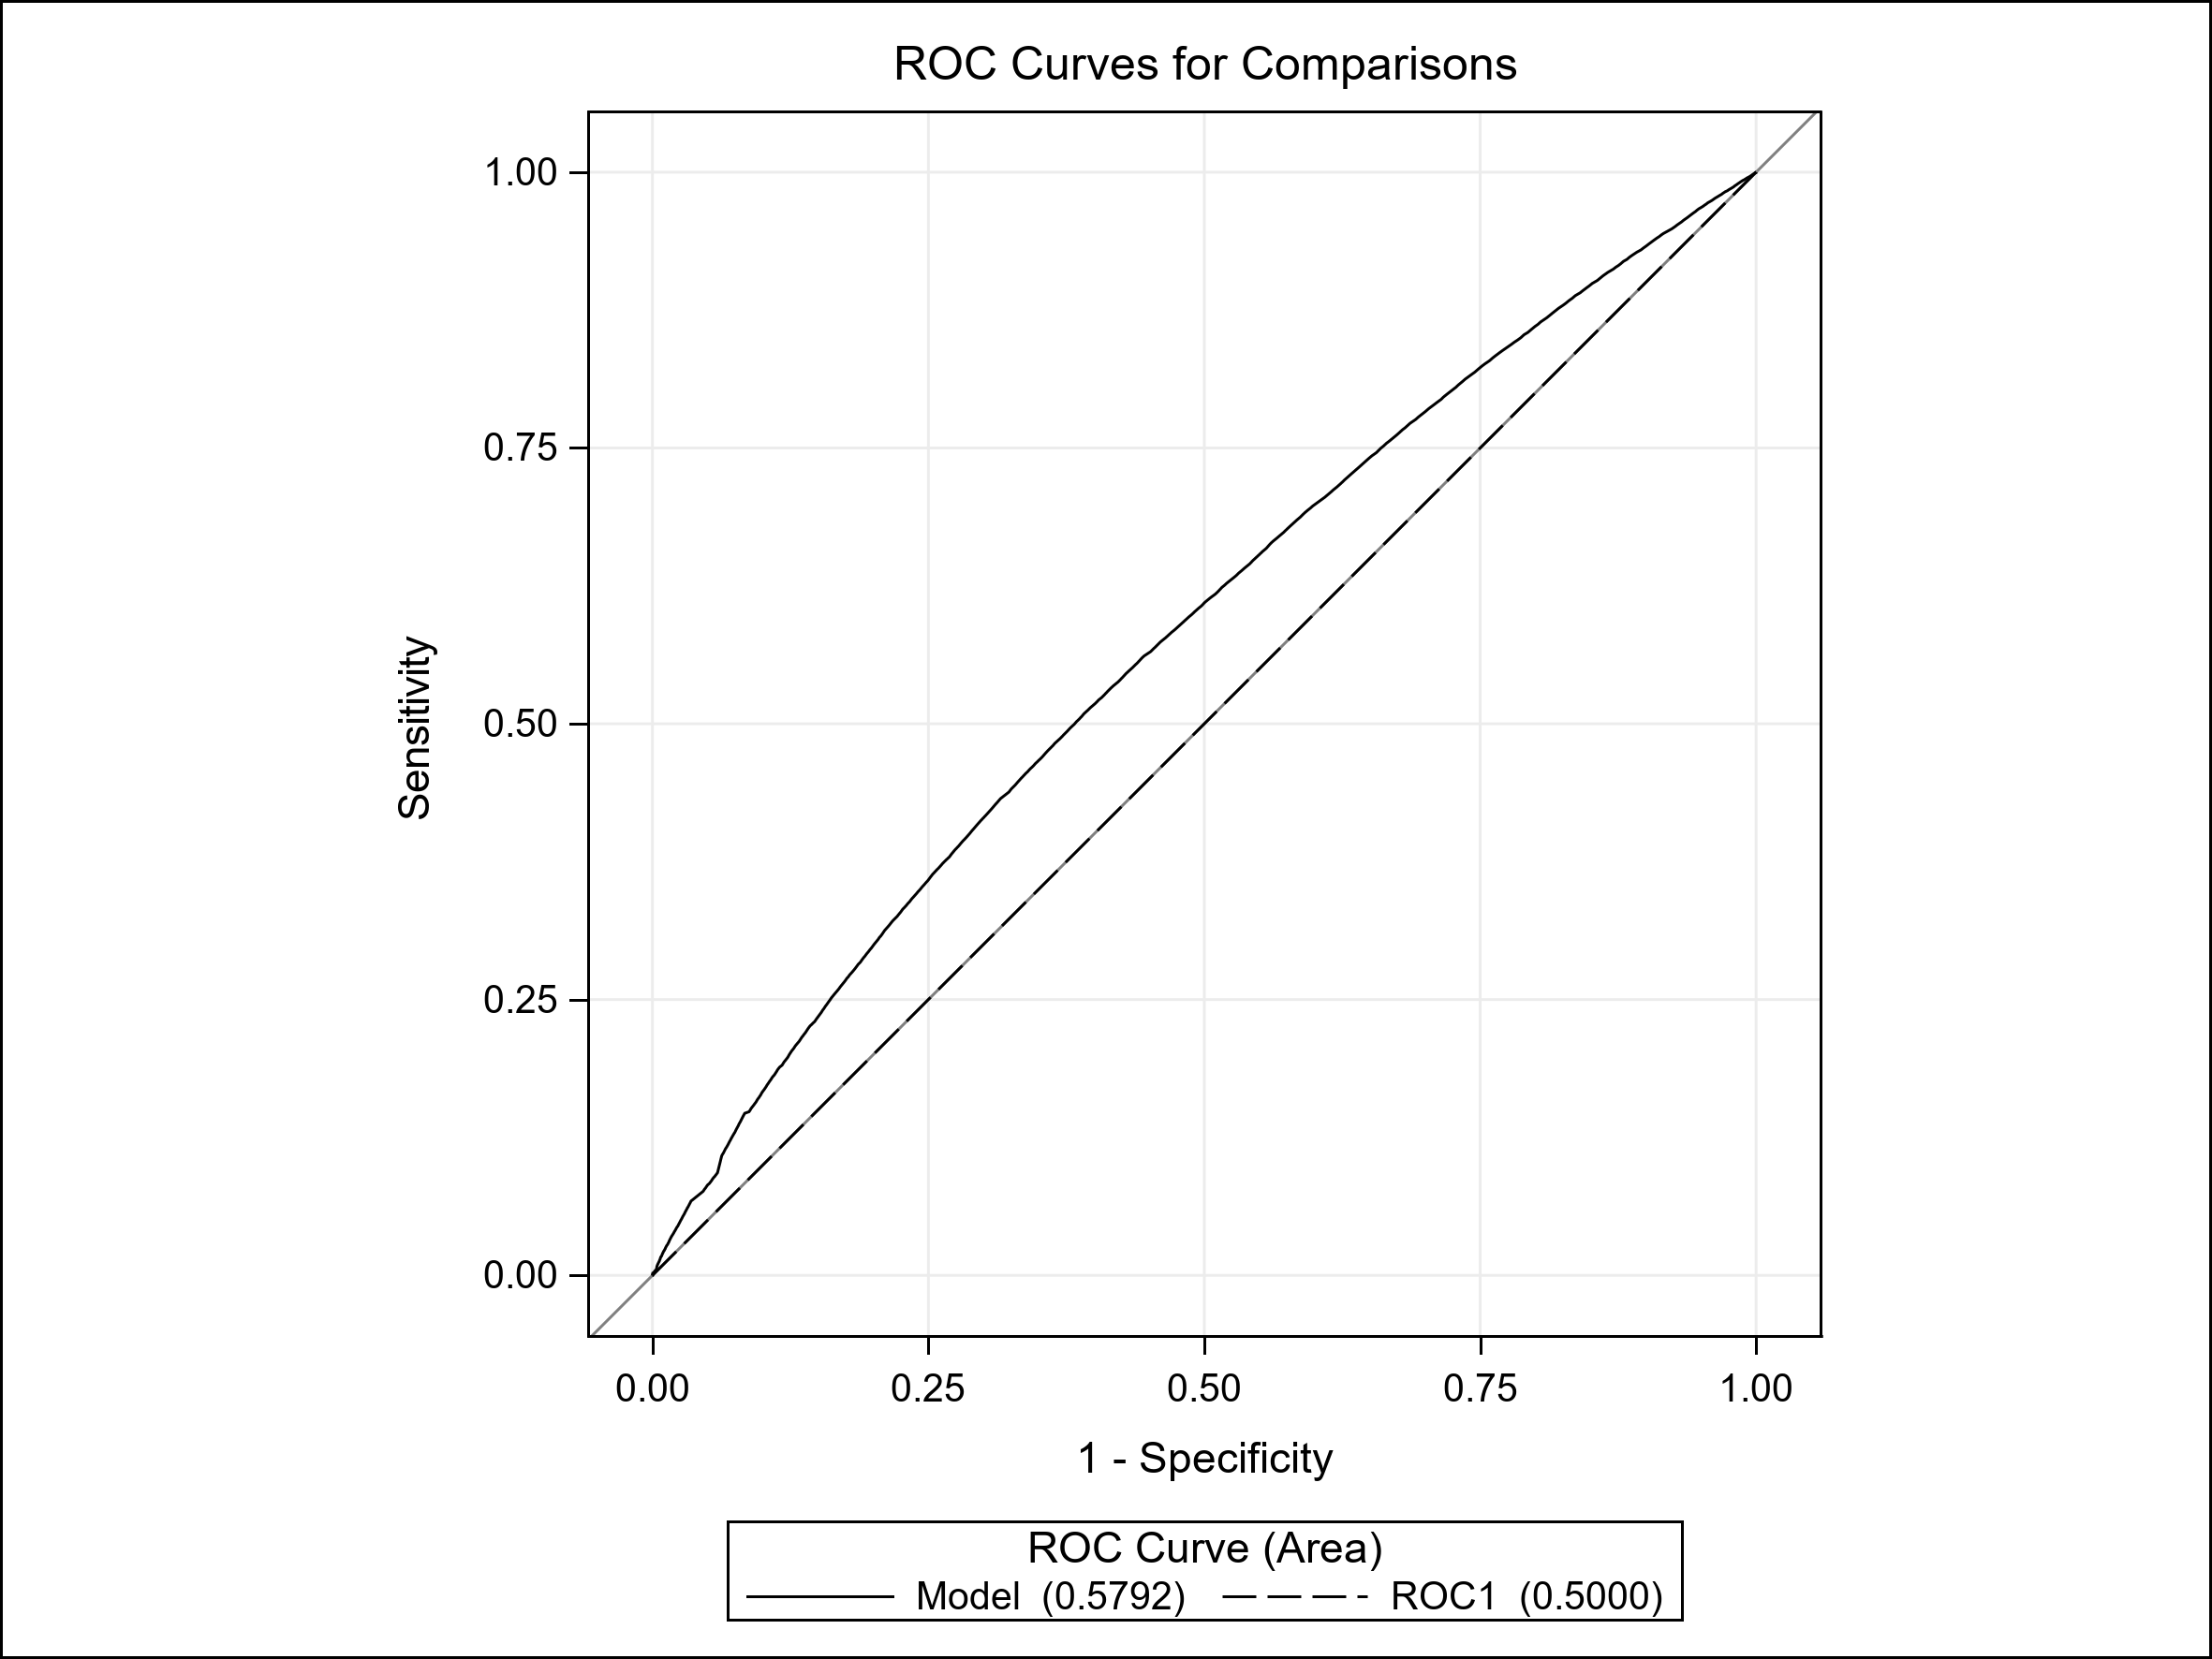
\includegraphics[width=0.9\textwidth]{./plot/ROC/Main/NUM_orig_upb_ROC_ALL5.png}
\end{minipage}
    \caption{ROC-curve of Credit Score (fico) and Original UPB}
    \label{fig:re_fico_upb}
\end{figure}
\begin{figure}[H]
\begin{minipage}{.5\textwidth}
	\centering
	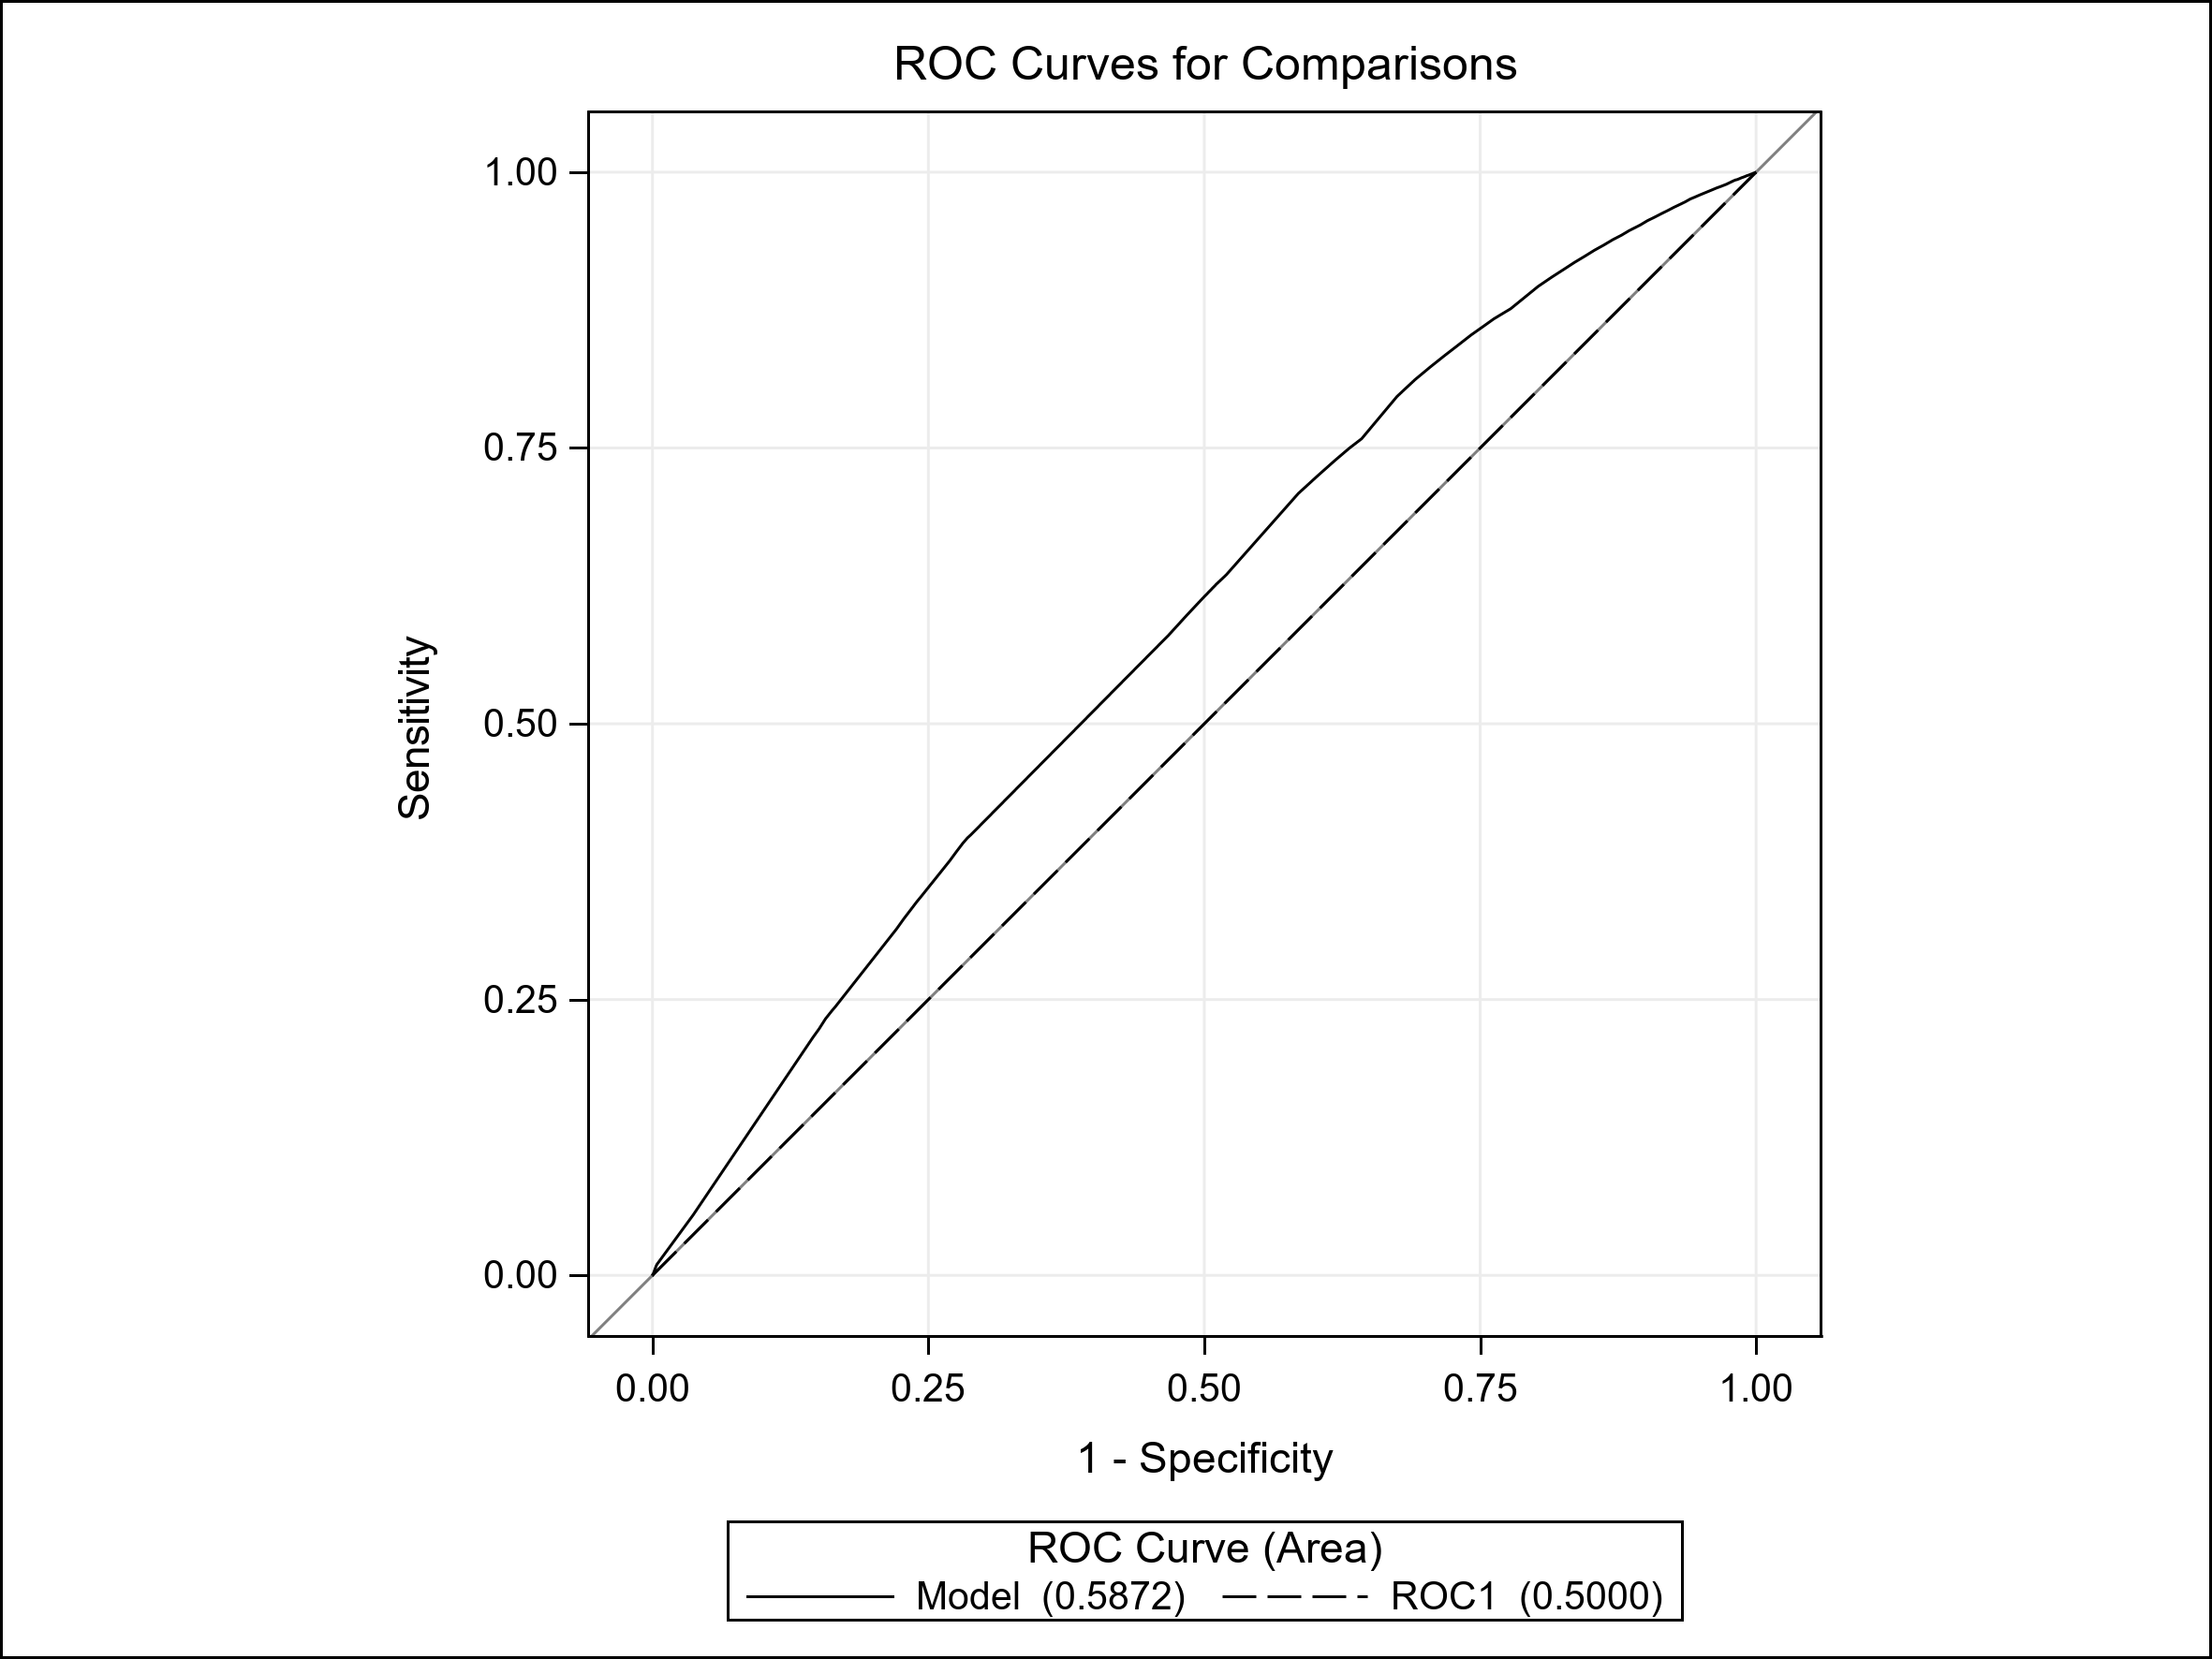
\includegraphics[width=0.9\textwidth]{./plot/ROC/Main/NUM_cltv_ROC_ALL5.png}
\end{minipage}%
\begin{minipage}{.5\textwidth}
	\centering
	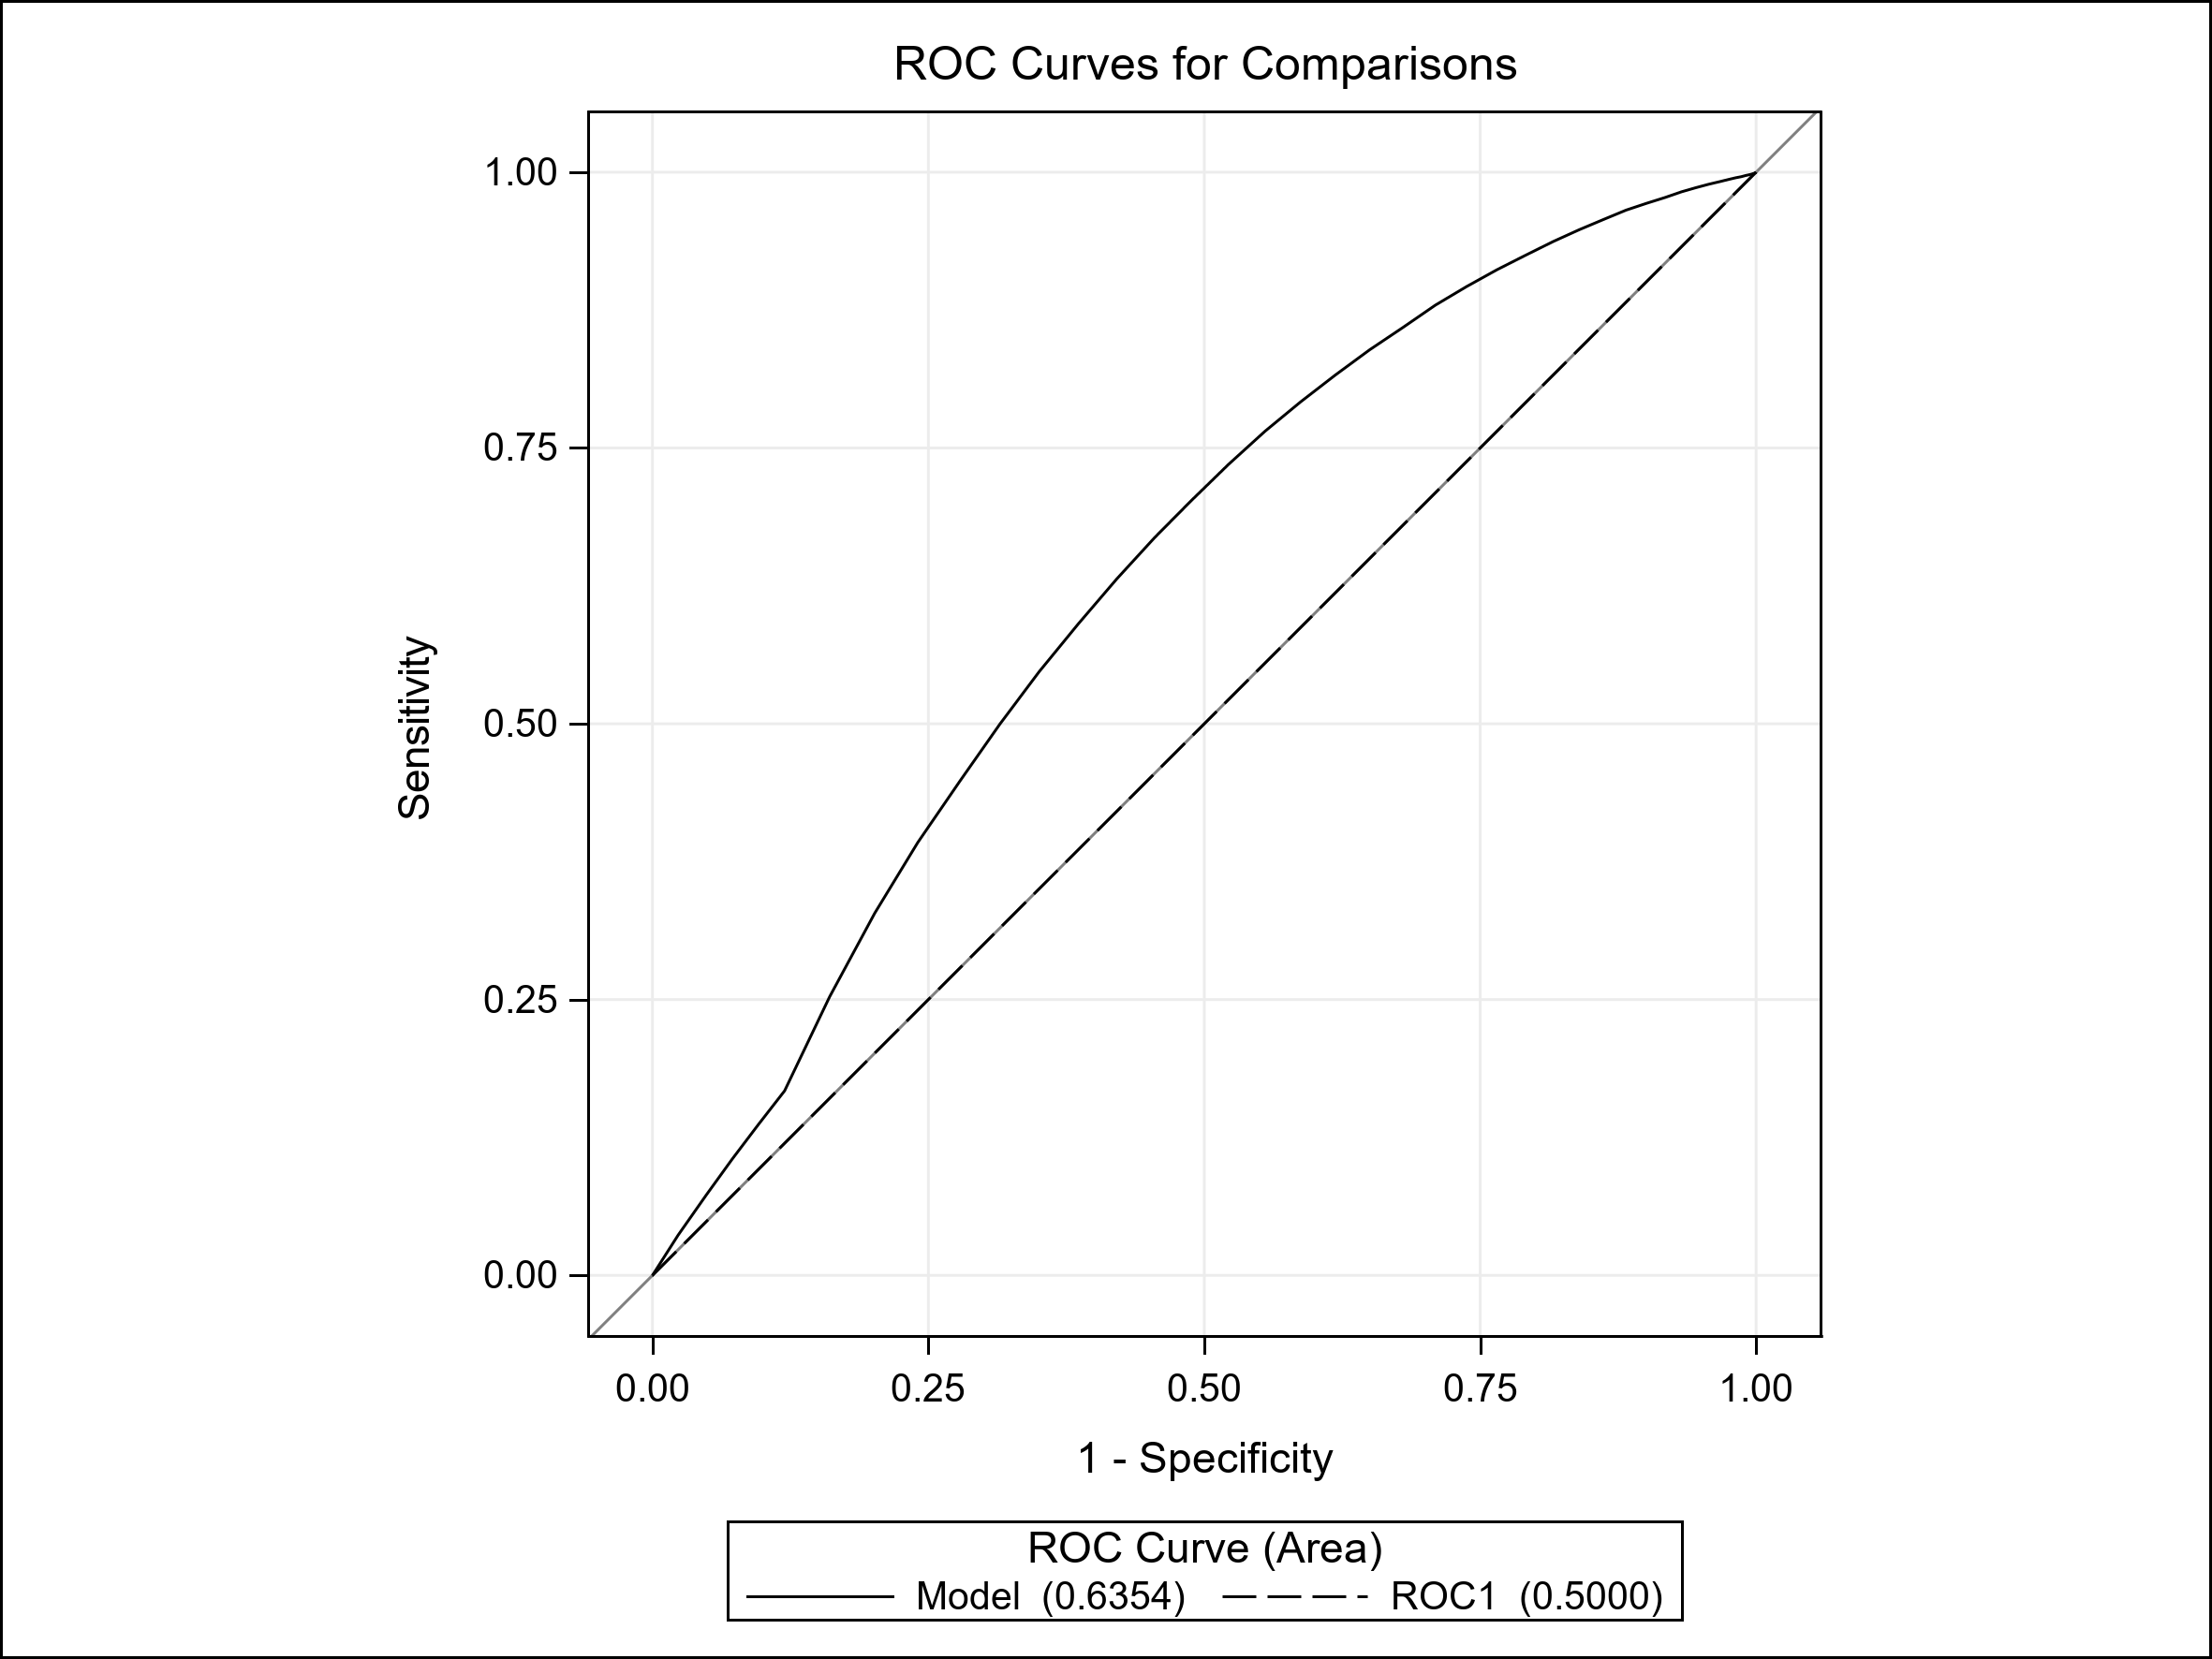
\includegraphics[width=0.9\textwidth]{./plot/ROC/Main/NUM_dti_ROC_ALL5.png}
\end{minipage}
    \caption{ROC-curve of CLTV and DTI}
    %\label{fig:dp_iqr_boxpl}
\end{figure}
\begin{figure}[H]
\begin{minipage}{.5\textwidth}
	\centering
	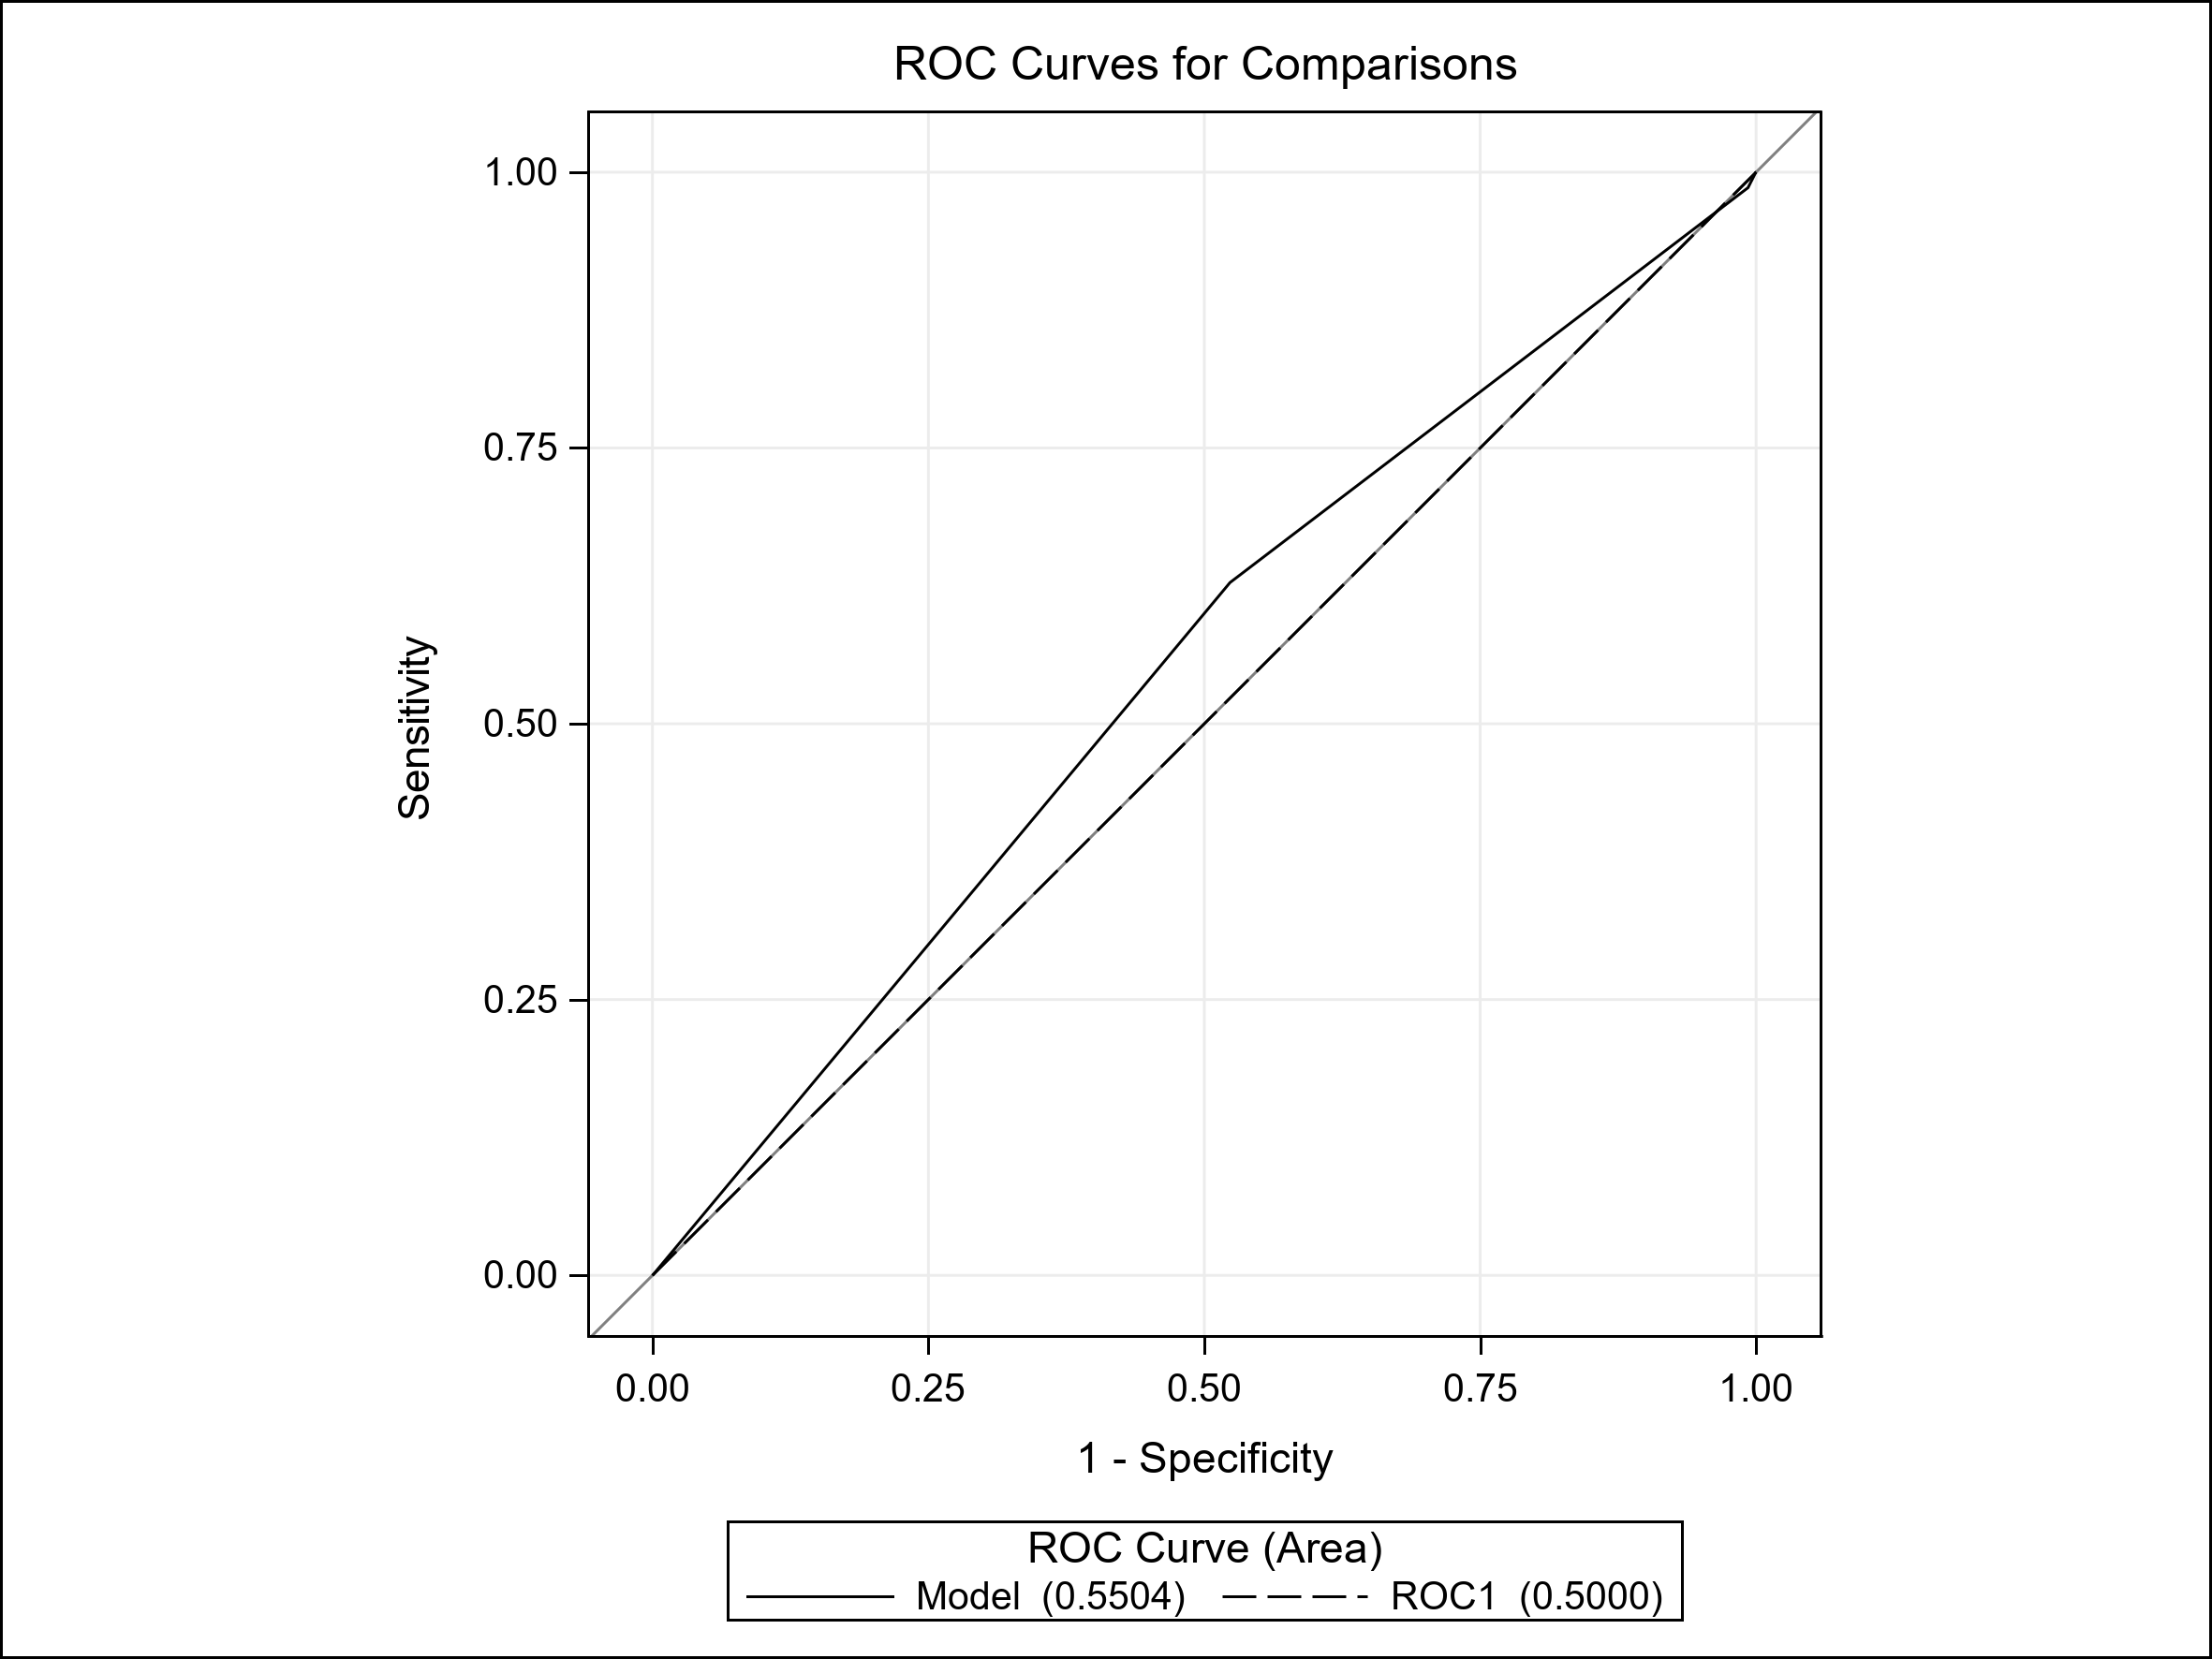
\includegraphics[width=0.9\textwidth]{./plot/ROC/Main/NUM_cnt_borr_ROC_ALL5.png}
\end{minipage}%
\begin{minipage}{.5\textwidth}
	\centering
	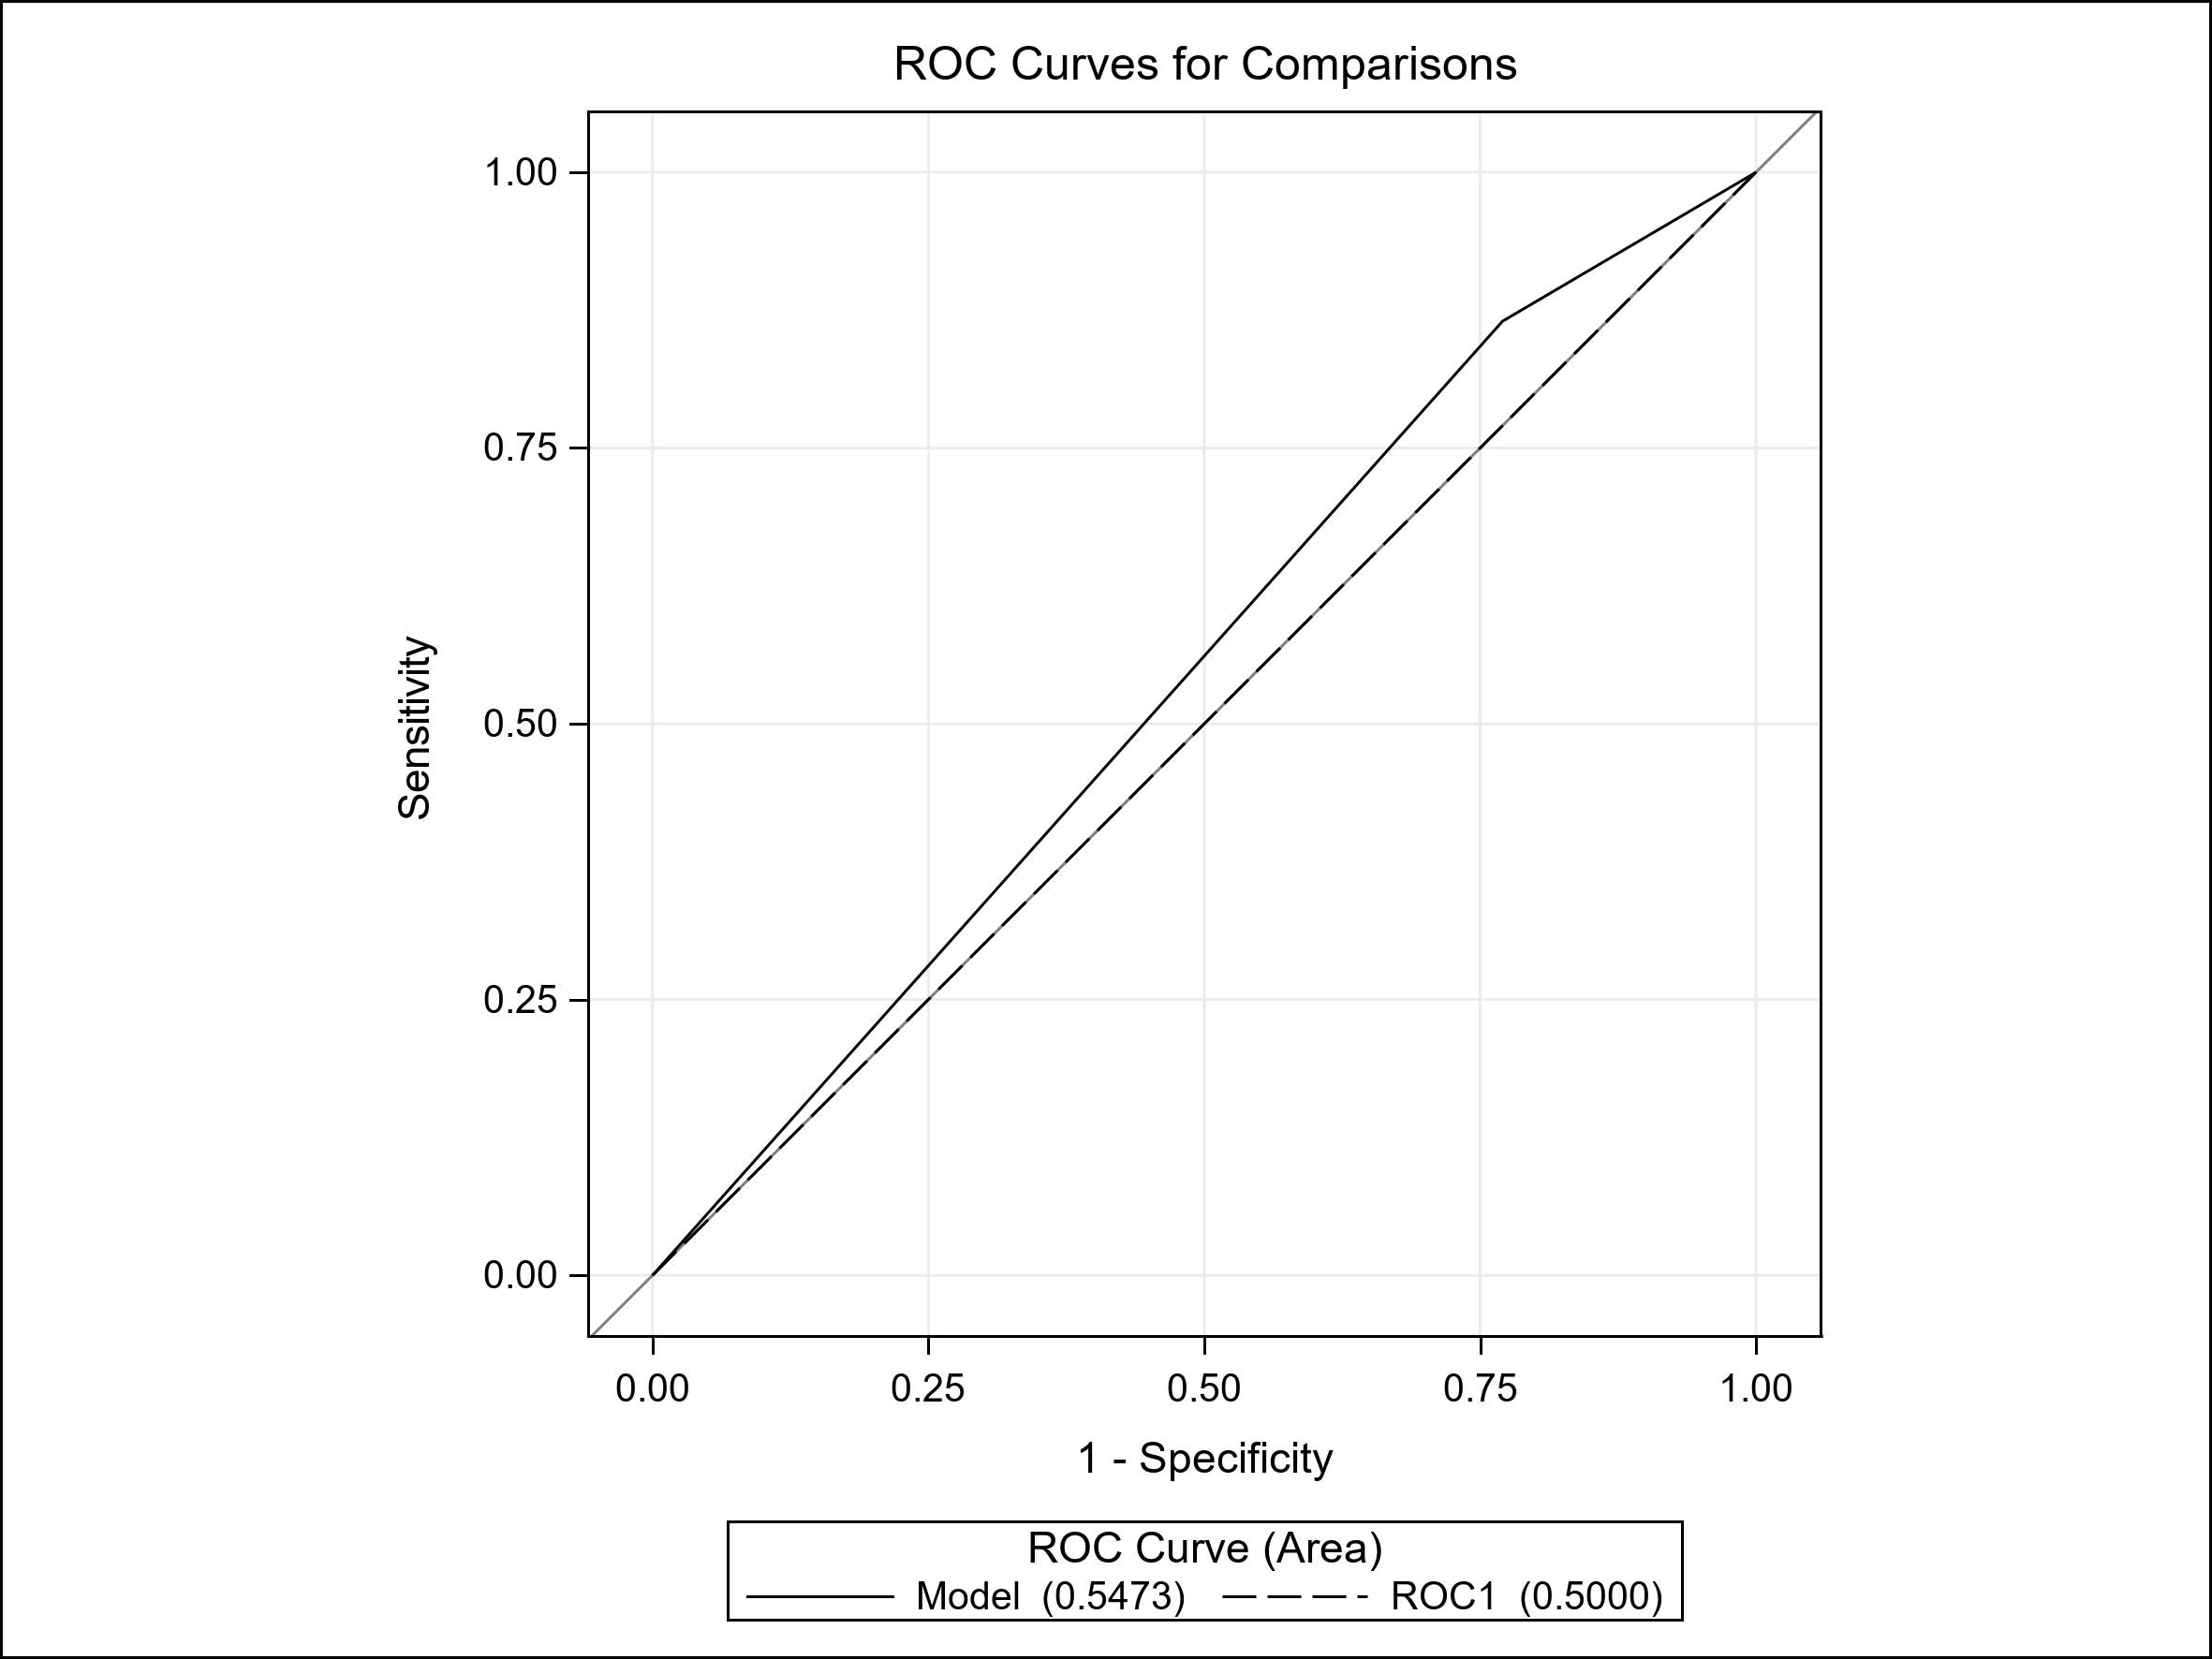
\includegraphics[width=0.9\textwidth]{./plot/ROC/Main/IND_flag_orig_loan_term_HEQ_360M_ROC_ALL5.png}
\end{minipage}
    \caption{ROC-curve of Number of Borrowers and Original Loan Term $\geq$ 360 months}
    %\label{fig:dp_iqr_boxpl}
\end{figure}
\begin{figure}[H]
\begin{minipage}{.5\textwidth}
	\centering
	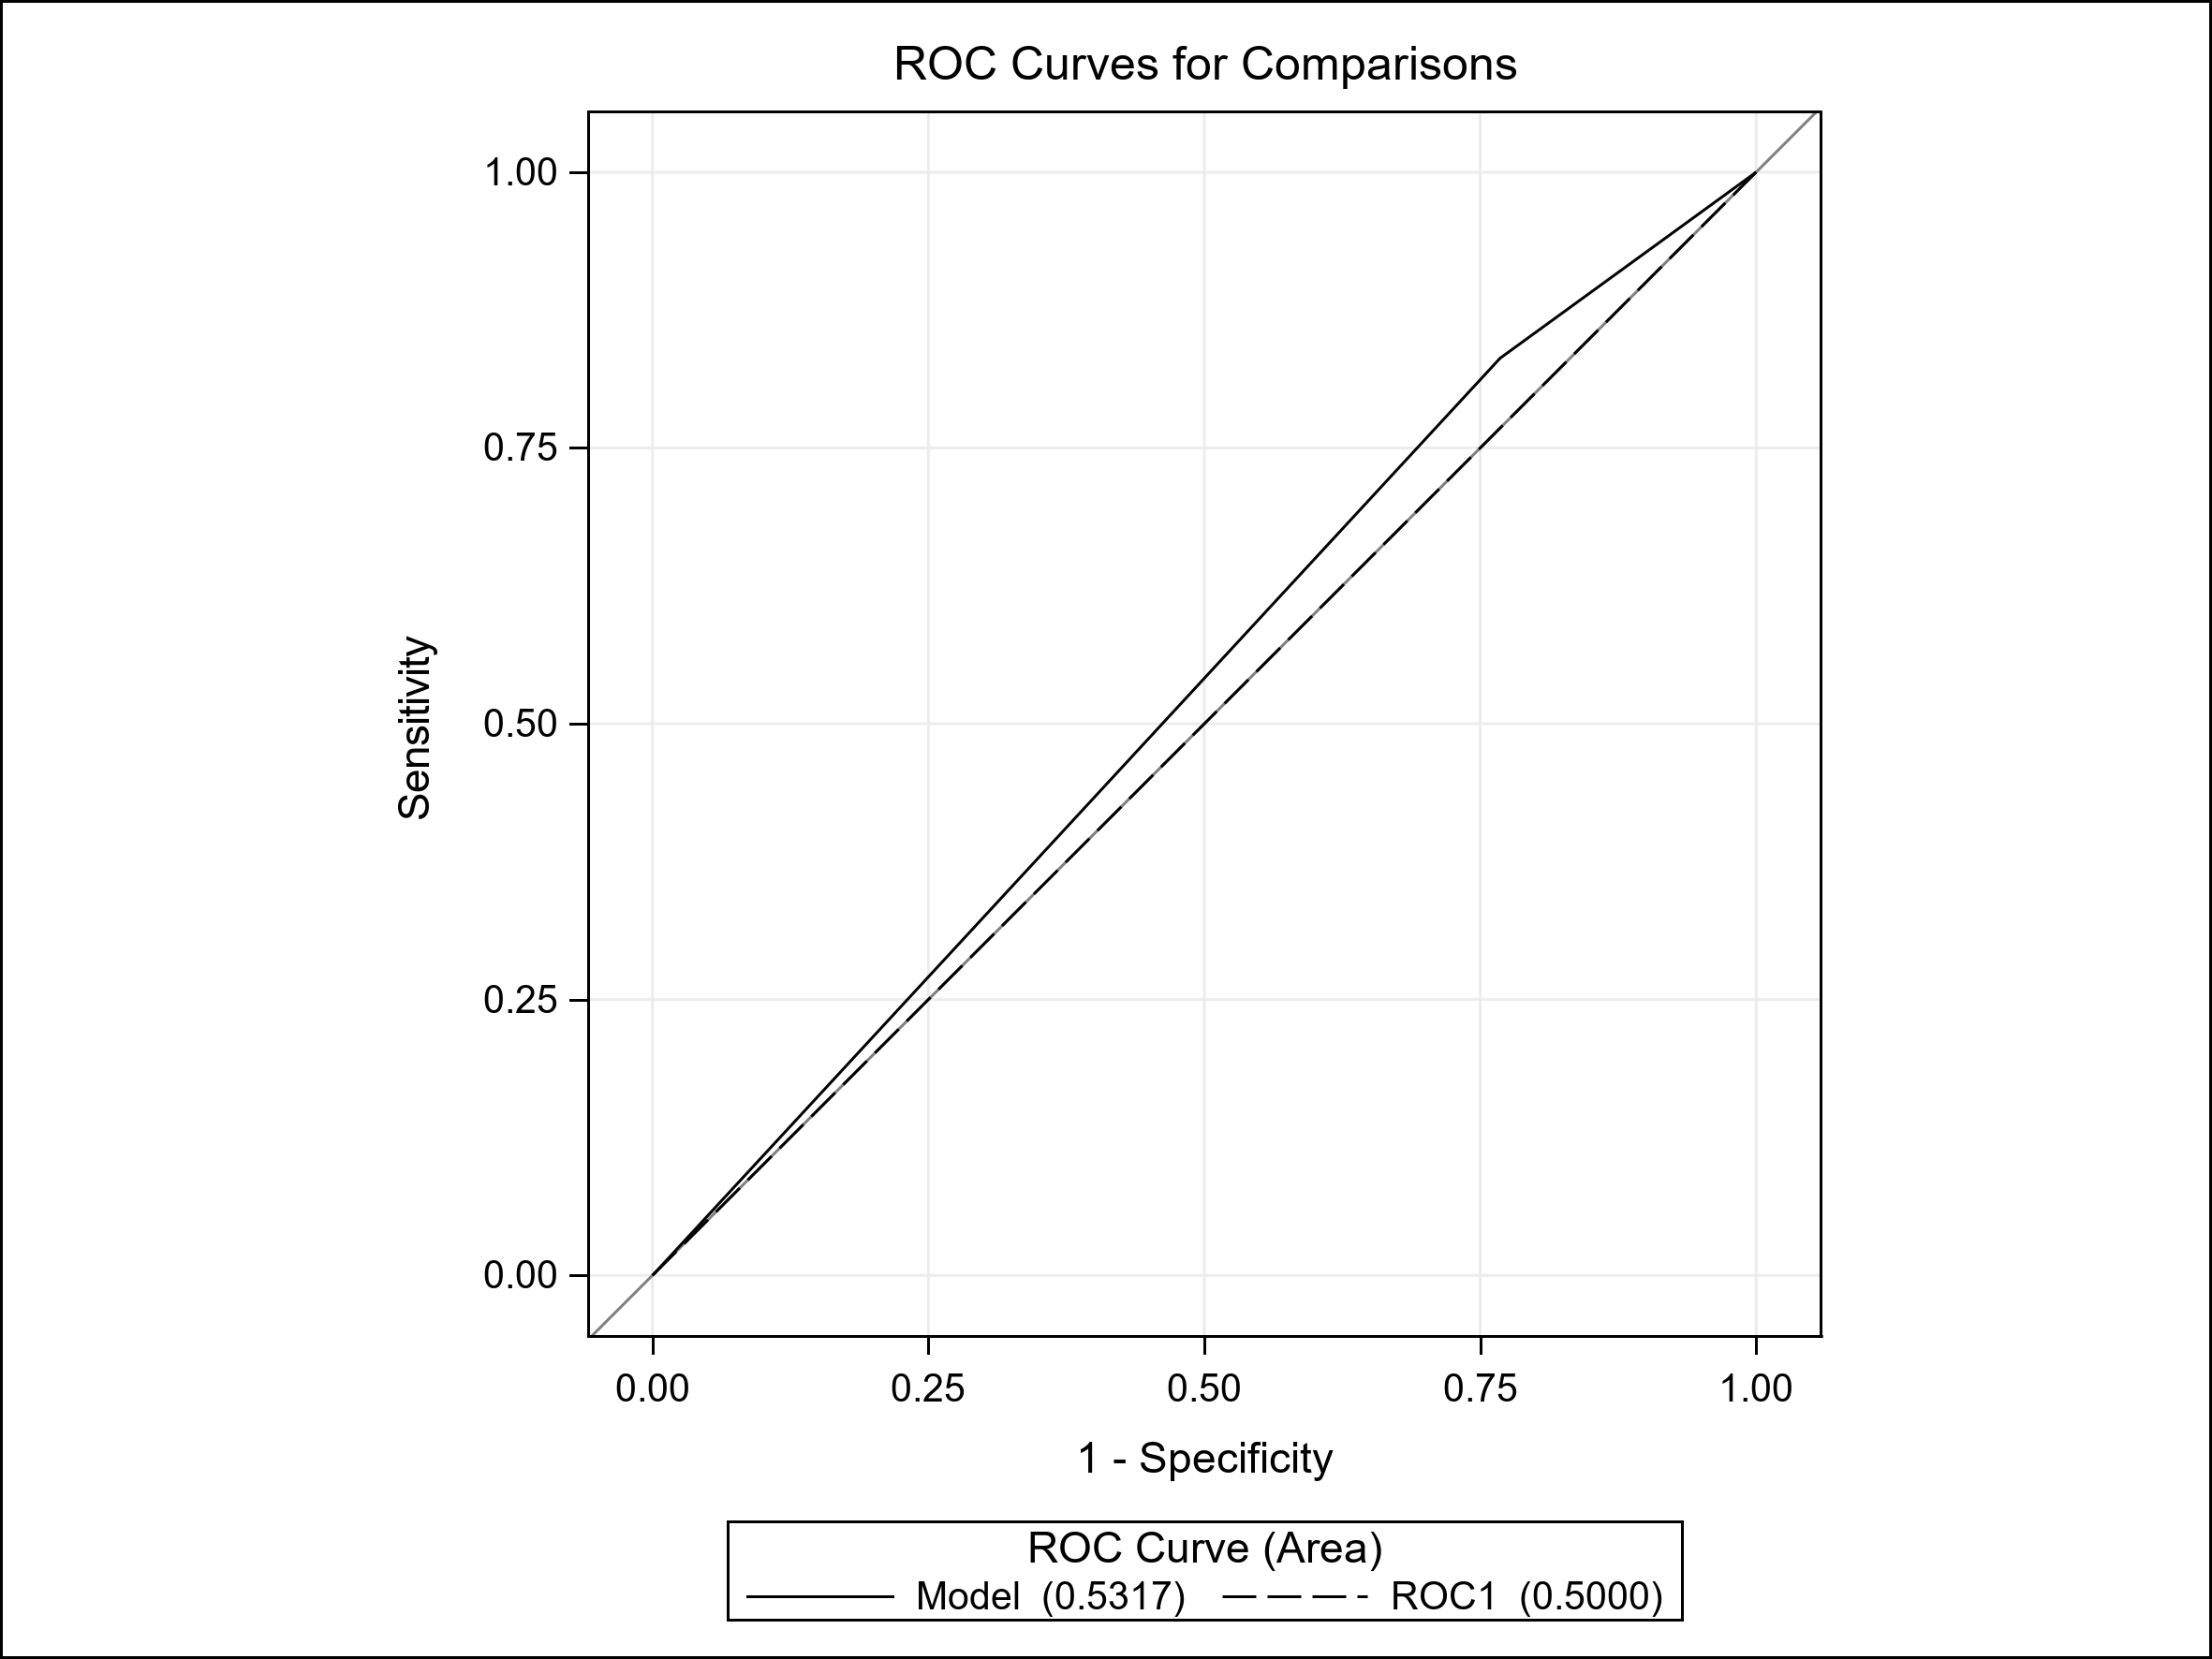
\includegraphics[width=0.9\textwidth]{./plot/ROC/Main/CAT_us_reg__Midwest_ROC_ALL5.png}
\end{minipage}%
\begin{minipage}{.5\textwidth}
	\centering
	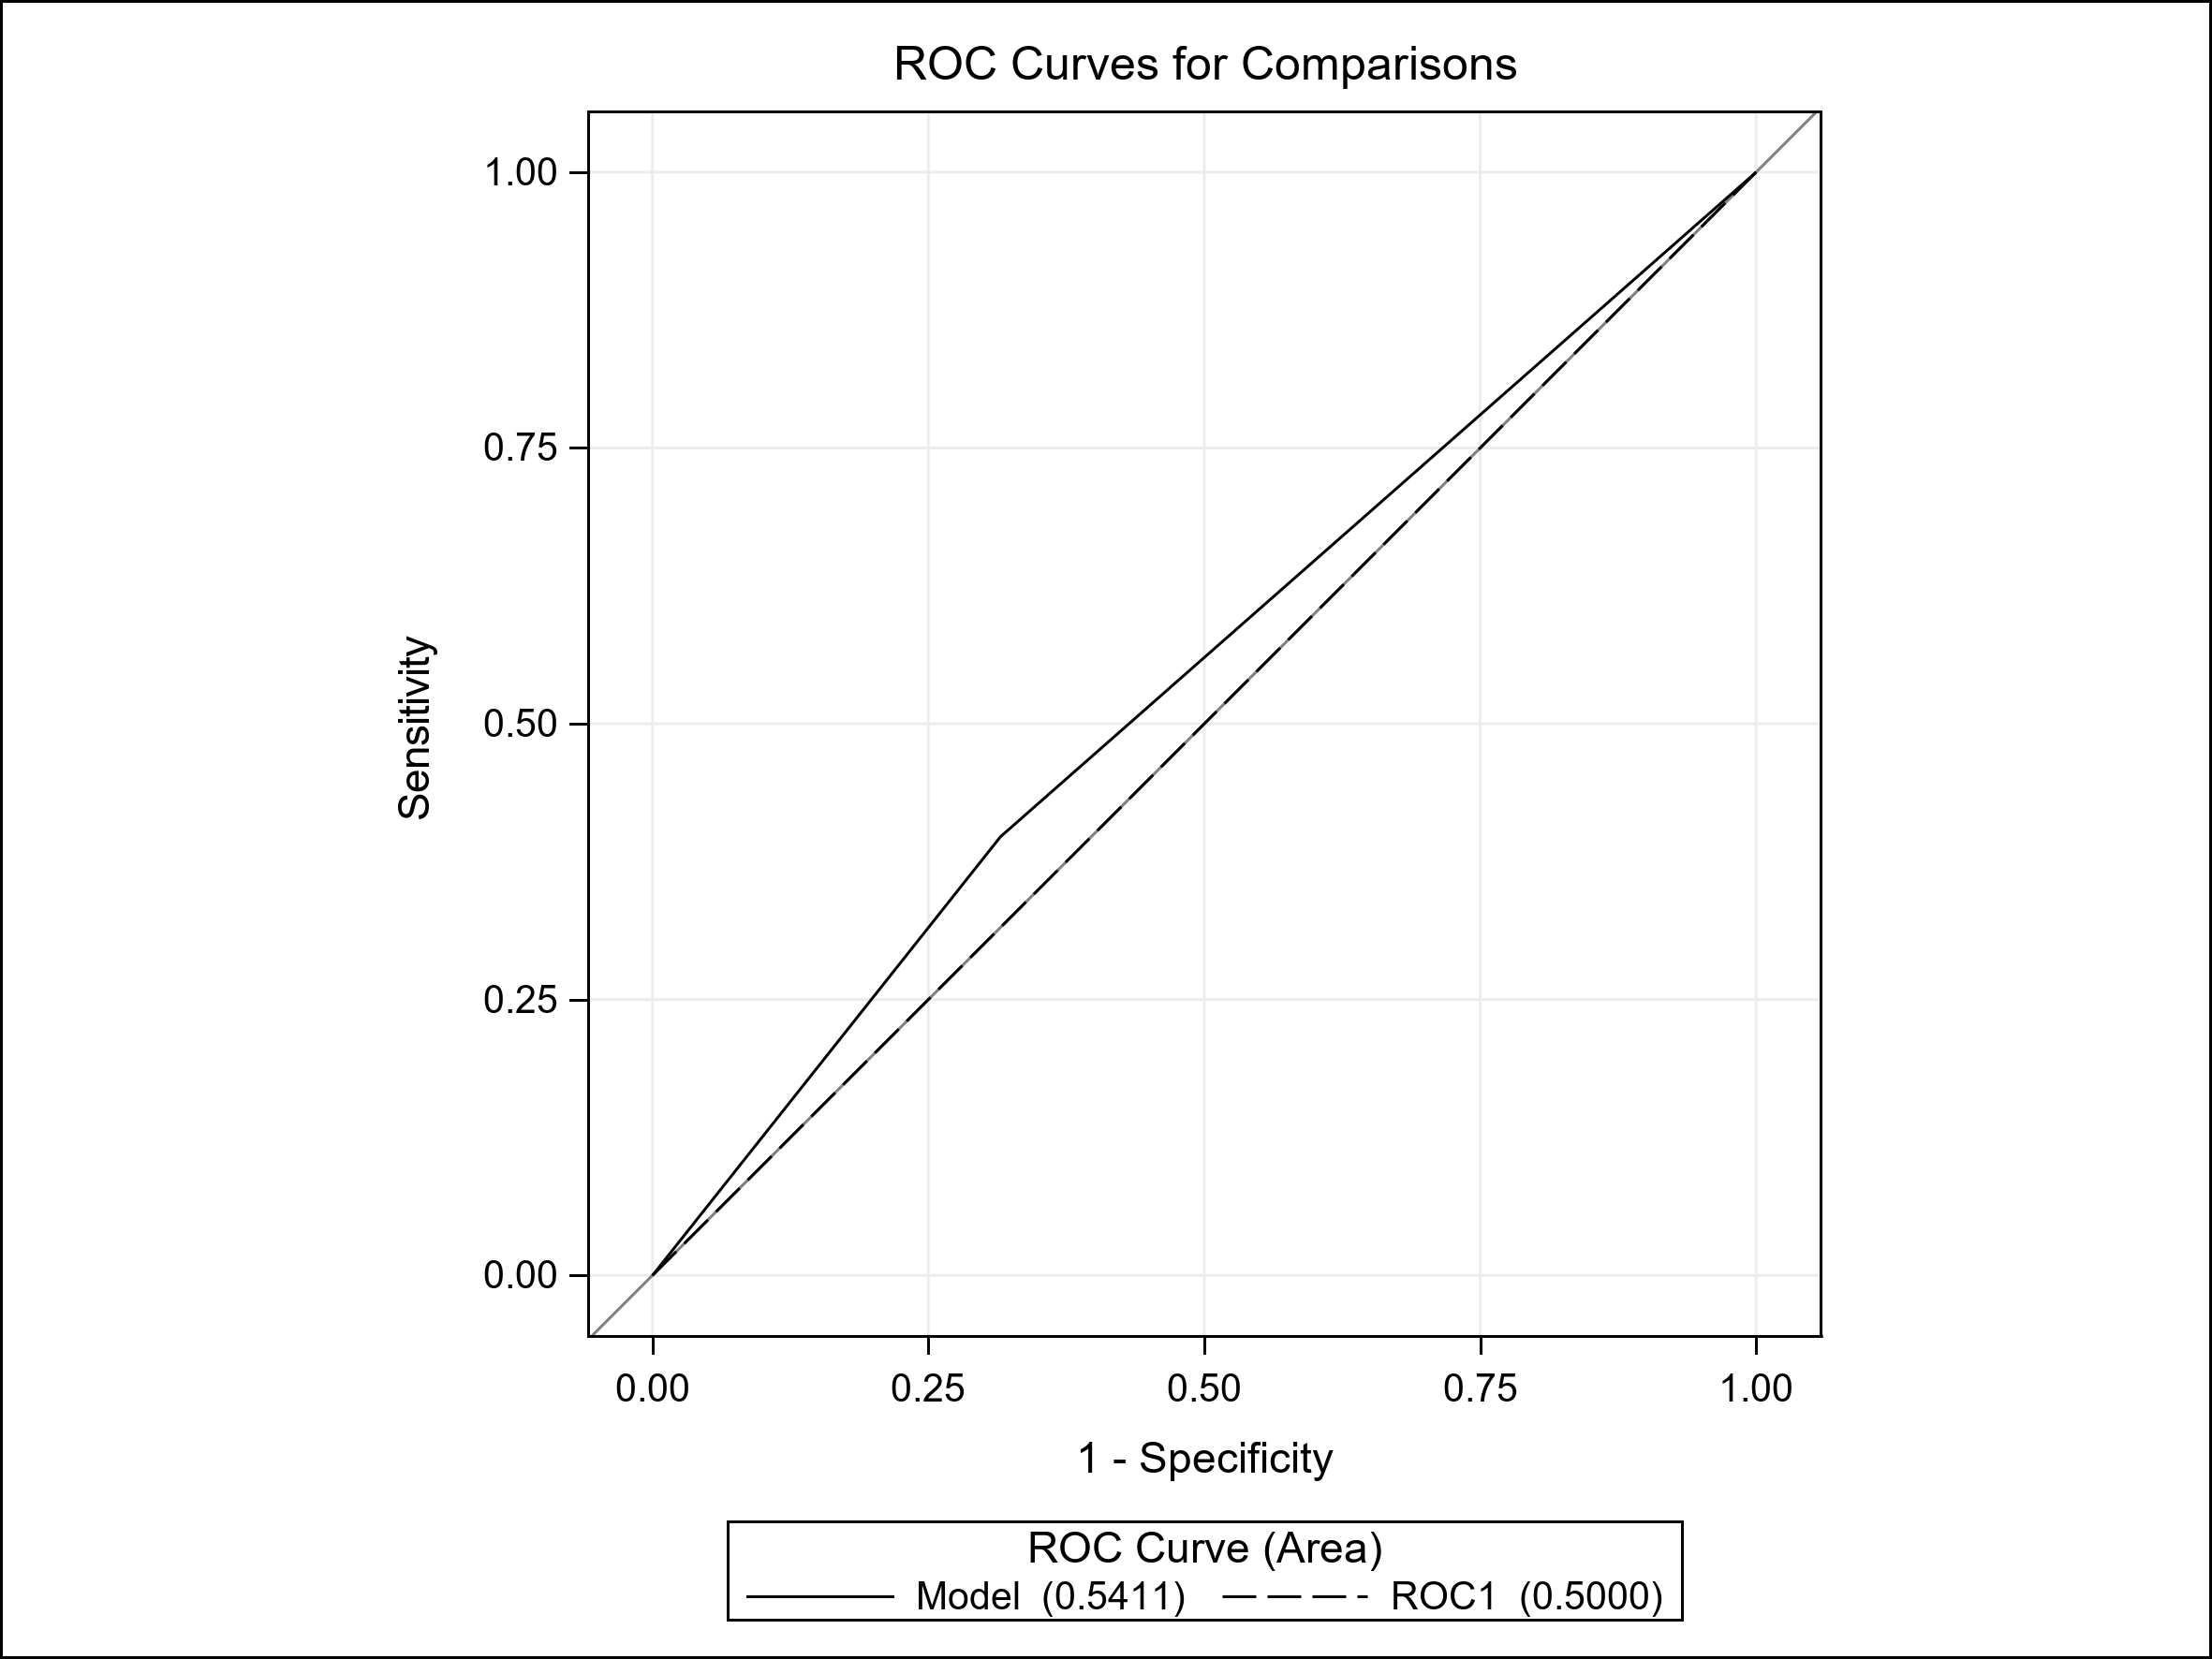
\includegraphics[width=0.9\textwidth]{./plot/ROC/Main/CAT_channel__C_ROC_ALL5.png}
\end{minipage}
    \caption{ROC-curve of US region = Midwest and Channel = Correspondent}
    \label{fig:re_usreg_channel}
\end{figure}

\newpage
\subsection{Multivariate Analysis}

The shortlist was created using the following process: First, the correlation matrix with all numerical variables was created. Then, the variable with the highest Gini coefficient was identified and all risk factors with a correlation coefficient above +0.25 or below -0.25 were removed. This step should be repeated with the remaining variables until all features were analyzed. 
Table \ref{tab:re_corr_matrix} shows the correlation coefficient for all numeric variables in the long list. To account for potential interaction effects between categorical and indicator variables, the Variance Inflation Factor (VIF) was considered. A high correlation coefficient between \emph{LTV} and \emph{CLTV} is expected and a higher correlation is also visible between \emph{MI Perc}, \emph{Loan Term}, \emph{LTV} and \emph{CLTV}. Executing the described process, \emph{CLTV} was added to the shortlist, while the remaining correlated risk factors were excluded.  The VIF values, as shown in Table \ref{tab:re_vif}, do not indicate severe multicollinearity. In the final step, the indicator version \emph{Loan Term $\geq$ 360m} was chosen instead of using the raw variable. The short list is given in Table \ref{tab:re_ll_sl}.

\begin{table}[H]
\resizebox{\textwidth}{!}{%
\begin{tabular}{ llllllllll }\toprule   
\textbf{Variable}     & \textbf{Credit Score} & \textbf{MI Perc}  & \textbf{No Units} & \textbf{CLTV}   & \textbf{DTI}   & \textbf{UPB} & \textbf{LTV} & \textbf{Loan Term} & \textbf{No Borrowers}\\\midrule
Credit Score & \cellcolor[HTML]{FFC7CE}{\color[HTML]{9C0006} 1,00} & -0,08                                               & 0,00                                                & -0,12                                               & -0,18                                               & 0,10                                                & -0,12                                               & -0,05                                               & -0,04                                               \\
MI Perc      & -0,08                                               & \cellcolor[HTML]{FFC7CE}{\color[HTML]{9C0006} 1,00} & -0,06                                               & \cellcolor[HTML]{FFC7CE}{\color[HTML]{9C0006} 0,67} & 0,10                                                & 0,03                                                & \cellcolor[HTML]{FFC7CE}{\color[HTML]{9C0006} 0,67} & \cellcolor[HTML]{FFC7CE}{\color[HTML]{9C0006} 0,26} & -0,05                                               \\
No Units     & 0,00                                                & -0,06                                               & \cellcolor[HTML]{FFC7CE}{\color[HTML]{9C0006} 1,00} & -0,05                                               & 0,04                                                & 0,06                                                & -0,05                                               & 0,02                                                & -0,02                                               \\
CLTV         & -0,12                                               & \cellcolor[HTML]{FFC7CE}{\color[HTML]{9C0006} 0,67} & -0,05                                               & \cellcolor[HTML]{FFC7CE}{\color[HTML]{9C0006} 1,00} & 0,13                                                & 0,09                                                & \cellcolor[HTML]{FFC7CE}{\color[HTML]{9C0006} 0,99} & \cellcolor[HTML]{FFC7CE}{\color[HTML]{9C0006} 0,33} & -0,06                                               \\
DTI          & -0,18                                               & 0,10                                                & 0,04                                                & 0,13                                                & \cellcolor[HTML]{FFC7CE}{\color[HTML]{9C0006} 1,00} & 0,06                                                & 0,13                                                & 0,13                                                & -0,08                                               \\
UPB          & 0,10                                                & 0,03                                                & 0,06                                                & 0,09                                                & 0,06                                                & \cellcolor[HTML]{FFC7CE}{\color[HTML]{9C0006} 1,00} & 0,09                                                & 0,16                                                & 0,15                                                \\
LTV          & -0,12                                               & \cellcolor[HTML]{FFC7CE}{\color[HTML]{9C0006} 0,67} & -0,05                                               & \cellcolor[HTML]{FFC7CE}{\color[HTML]{9C0006} 0,99} & 0,13                                                & 0,09                                                & \cellcolor[HTML]{FFC7CE}{\color[HTML]{9C0006} 1,00} & \cellcolor[HTML]{FFC7CE}{\color[HTML]{9C0006} 0,33} & -0,07                                               \\
Loan Term    & -0,05                                               & \cellcolor[HTML]{FFC7CE}{\color[HTML]{9C0006} 0,26} & 0,02                                                & \cellcolor[HTML]{FFC7CE}{\color[HTML]{9C0006} 0,33} & 0,13                                                & 0,16                                                & \cellcolor[HTML]{FFC7CE}{\color[HTML]{9C0006} 0,33} & \cellcolor[HTML]{FFC7CE}{\color[HTML]{9C0006} 1,00} & -0,06                                               \\
No Borrowers & -0,04                                               & -0,05                                               & -0,02                                               & -0,06                                               & -0,08                                               & 0,15                                                & -0,07                                               & -0,06                                               & \cellcolor[HTML]{FFC7CE}{\color[HTML]{9C0006} 1,00}           \\\bottomrule
\end{tabular}%
}
\caption{Correlation matrix}
\label{tab:re_corr_matrix}   
\end{table}

\begin{table}[H]
\centering
\begin{tabular}{p{8cm}cc}\toprule   
\textbf{Variable}                                                                & \textbf{VIF} 					& \textbf{p-value} \\\midrule
Credit Score                                                                     & 1,09                             & \textless{}.0001                     \\
DTI                                                                              & 1,09                             & \textless{}.0001                     \\
CLTV                                                                             & 2,08                             & \textless{}.0001                     \\
No Borrowers                                                                     & 1,02                             & \textless{}.0001                     \\
No Units                                                                         & 1,09                             & \textless{}.0001                     \\
Homebuyer Flag                                                                   & 1,57                             & \textless{}.0001                     \\
MI Flag                                                                          & 2,02                             & \textless{}.0001                     \\
Loan Term $\geq$ 360m                                                            & 1,22                             & \textless{}.0001                     \\
Channel = Not Available                                                          & 1,00                             & 0.7367                               \\
Channel = Broker                                                                 & 1,10                             & \textless{}.0001                     \\
Channel = Correspondent                                                          & 1,09                             & \textless{}.0001                     \\
Loan Purpose = Refinance - Cash Out    											 & 1,71                             & \textless{}.0001                     \\
Loan Purpose = Refinance - No Cash Out 											 & 2,08                             & \textless{}.0001                     \\
Prop Val Method = ACE Loans                                                      & 1,49                             & \textless{}.0001                     \\
Prop Val Method = Other Appraisals (Desktop, driveby, external, AVM)             & 1,03                             & \textless{}.0001                     \\
Prop Val Method = Not Available                                                  & 1,00                             & 0.6436                               \\
US Region = Midwest                                                              & 1,30                             & \textless{}.0001                     \\
US Region = Northeast                                                            & 1,23                             & \textless{}.0001                     \\
US Region = Other                                                                & 1,00                             & \textless{}.0001                     \\
US Region = West                                                                 & 1,40                             & \textless{}.0001                     \\
Occupancy = Second Home                                                          & 1,06                             & 0.0103                               \\
Occupancy = Investment Property                                                  & 1,16                             & \textless{}.0001                    \\\bottomrule
\end{tabular}
\caption{Variance Inflation Factor}
\label{tab:re_vif}   
\end{table}

\begin{longtable}{ l c c }\toprule    
\textbf{Variable}           & \textbf{Long List} 											& \textbf{Short List}						 \\\midrule
Credit Score                & \cellcolor[HTML]{C0F0C0}Missing Treatment applied            & \cellcolor[HTML]{C0F0C0}                     \\
Homebuyer Flag              & \cellcolor[HTML]{F7D9E1}Low Gini                             & -                                            \\
MI Perc                     & \cellcolor[HTML]{C0F0C0}Missing Treatment applied            & \cellcolor[HTML]{F7D9E1}Correlated with CLTV \\
No Units                    & \cellcolor[HTML]{F7D9E1}Low Gini                             & -                                            \\
Occupancy                   & \cellcolor[HTML]{F7D9E1}Low Gini                             & -                                            \\
CLTV                        & \cellcolor[HTML]{C0F0C0}Missing Treatment applied            & \cellcolor[HTML]{C0F0C0}                     \\
DTI                         & \cellcolor[HTML]{C0F0C0}Missing Treatment applied            & \cellcolor[HTML]{C0F0C0}                     \\
UPB                         & \cellcolor[HTML]{C0F0C0}                                     & \cellcolor[HTML]{C0F0C0}                     \\
LTV                         & \cellcolor[HTML]{C0F0C0}Missing Treatment applied            & \cellcolor[HTML]{F7D9E1}Correlated with CLTV \\
Channel                     & \cellcolor[HTML]{C0F0C0}                                     & \cellcolor[HTML]{C0F0C0}                     \\
PPM Flag                    & \cellcolor[HTML]{F7D9E1}Low Gini                             & -                                            \\
Amort Type                  & \cellcolor[HTML]{F7D9E1}Low Gini                             & -                                            \\
State                       & \cellcolor[HTML]{F7D9E1}Adapted Variable derived (US-region) & -                                            \\
Prop Type                   & \cellcolor[HTML]{F7D9E1}Low Gini                             & -                                            \\
Loan Purpose                & \cellcolor[HTML]{F7D9E1}Low Gini                             & -                                            \\
Loan Term                   & \cellcolor[HTML]{C0F0C0}                                     & \cellcolor[HTML]{F7D9E1}Correlated with CLTV \\
No Borrowers                & \cellcolor[HTML]{C0F0C0}                                     & \cellcolor[HTML]{C0F0C0}                     \\
Sup Conf Flag               & \cellcolor[HTML]{F7D9E1}High Missing Rate                    & -                                            \\
Prog Flag                   & \cellcolor[HTML]{F7D9E1}High Missing Rate                    & -                                            \\
HARP Flag                   & \cellcolor[HTML]{F7D9E1}High Missing Rate                    & -                                            \\
Prop Val Method             & \cellcolor[HTML]{C0F0C0}                                     & \cellcolor[HTML]{C0F0C0}                     \\
Int Only Flag               & \cellcolor[HTML]{F7D9E1}Low Gini                             & -                                            \\
US Region                   & \cellcolor[HTML]{C0F0C0}                                     & \cellcolor[HTML]{C0F0C0}                     \\
MI Flag                     & \cellcolor[HTML]{C0F0C0}                                     & \cellcolor[HTML]{C0F0C0}                     \\
Loan Term \textgreater 360m & \cellcolor[HTML]{F7D9E1}Low Gini                             & -                                            \\
Loan Term Group             & \cellcolor[HTML]{F7D9E1}Similar Variable used                & -                                            \\
Loan Term $\geq$ 360m       & \cellcolor[HTML]{C0F0C0}                                     & \cellcolor[HTML]{C0F0C0}                     \\
Loan Term = 360m            & \cellcolor[HTML]{F7D9E1}Similar Variable used                & -                                           \\\bottomrule
\caption{Long list and Short list}
\label{tab:re_ll_sl}       
\end{longtable}

\subsection{Scaling}
Due to the different ranges of risk factors, especially because of \emph{Original Unpaid Balance}, a standardization of all numeric variables was carried out to prevent unusually small or large coefficients and enhance the comparability of the model coefficients. The following formula is used:

\begin{equation}
X_{\text{standardized}} = \frac{X - \mu}{\sigma}
\end{equation}
where:
\begin{conditions}
 X  	& original variable \\
\mu		& mean of the variable \\
\sigma	& standard deviation of the variable
\end{conditions}

\section{Modeling}

\subsection{Logistic Regression}
Employing the forward stepwise selection algorithm, all short list variables were inserted into the modeling process, resulting in the model presented in Table \ref{tab:re_prelLogModel}. The order of the risk factors indicates the significance in the model, with all coefficients exhibiting statistical significance indicated by low p-values. The AIC and BIC were calculated at each modeling step to limit the number of explanatory variables. Table \ref{tab:re_AICBIC} outlines the relative change per step. A noticeable drop in improvement occurs between step 5 and 6 and thus, prompting the removal of all succeeding variables, followed by a re-estimation of the model. The final model, detailed in Table \ref{tab:re_finalLogModel}, only includes numeric variables. All coefficients align with the expected economic sign; for example, a higher DTI corresponds to a higher \acl{PD}, reflected in a positive coefficient. In contrast, an increased number of borrowers, which means more people are obligated to repay the loan, correlates with a lower \acl{PD}, resulting in a negative coefficient. Performance metrics for the model are provided in Chapter \ref{sec:comp_model} as part of the comparison with the Random Forest model.

\begin{table}[H]
\centering
\begin{tabular}{p{8cm}rr}\toprule
\textbf{Parameter}                                                   & \textbf{Coefficient} & \textbf{p-value} \\\midrule
Intercept                                                            & -4,892               & \textless{}.0001 \\
Credit Score                                                         & -0,542               & \textless{}.0001 \\
DTI                                                         		 & 0,392                & \textless{}.0001 \\
CLTV                                                                 & 0,223                & \textless{}.0001 \\
UPB                                                                  & 0,316                & \textless{}.0001 \\
No Borrowers                                                         & -0,245               & \textless{}.0001 \\
Loan Term $\geq$ 360m                                                & 0,144                & \textless{}.0001 \\
Channel = Broker                                                     & 0,104                & \textless{}.0001 \\
Channel = Correspondent                                              & 0,279                & \textless{}.0001 \\
Prop Val Method = Other Appraisals (Desktop, driveby, external, AVM) & -0,206               & \textless{}.0001 \\
Prop Val Method = Full Appraisal                                     & 0,180                & \textless{}.0001 \\
US Region = Midwest                                                  & -0,152               & \textless{}.0001 \\
US Region = Northeast                                                & 0,138                & \textless{}.0001 \\
US Region = Other                                                    & 0,869                & \textless{}.0001\\\bottomrule
\end{tabular}
\caption{Preliminary Logit Model}
\label{tab:re_prelLogModel}
\end{table}

\begin{table}[H]
\centering
\begin{tabular}{lccccp{4cm}}\toprule
\textbf{Step} & \textbf{AIC} & \textbf{rel. AIC ch.} & \textbf{BIC} & \textbf{rel. BIC ch.} & \textbf{Variable added}                                              \\\midrule
1             & 577821       &                       & 577847       &                       & Credit Score                                                         \\
2             & 568369       & -1,64\%               & 568408       & -1,63\%               & DTI adjusted                                                         \\
3             & 562335       & -1,06\%               & 562388       & -1,06\%               & CLTV                                                                 \\
4             & 558885       & -0,61\%               & 558951       & -0,61\%               & UPB                                                                  \\
5             & 555949       & -0,53\%               & 556028       & -0,52\%               & No Borrowers                                                         \\
6             & 554913       & -0,19\%               & 555005       & -0,18\%               & Loan Term $\geq$ 360m                                                 \\
7             & 554574       & -0,06\%               & 554679       & -0,06\%               & Channel = Broker                                                     \\
8             & 554308       & -0,05\%               & 554427       & -0,05\%               & Channel = Correspondent                                              \\
9             & 554193       & -0,02\%               & 554324       & -0,02\%               & Prop Val Method = Other Appraisals (Desktop, driveby, external, AVM) \\
10            & 554066       & -0,02\%               & 554210       & -0,02\%               & Prop Val Method = Full Appraisal                                     \\
11            & 554008       & -0,01\%               & 554166       & -0,01\%               & US Region = Midwest                                                  \\
12            & 553984       & 0,00\%                & 554155       & 0,00\%                & US Region = Northeast                                                \\
13            & 553953       & -0,01\%               & 554137       & 0,00\%                & US Region = Other                                                   \\\bottomrule
\end{tabular}
\caption{AIC and BIC per step}
\label{tab:re_AICBIC}
\end{table}

\begin{table}[H]
\centering
\begin{tabular}{lrr}\toprule
\textbf{Parameter}     	& \textbf{Coefficient} & \textbf{p-value} \\\midrule
Intercept          		& -4,546               & \textless{}.0001 \\
Credit Score       		& -0,542               & \textless{}.0001 \\
DTI adjusted       		& 0,408                & \textless{}.0001 \\
CLTV               		& 0,261                & \textless{}.0001 \\
No Borrowers       		& -0,248               & \textless{}.0001 \\
UPB                		& 0,341                & \textless{}.0001\\\bottomrule
\end{tabular}
\caption{Final Logit Model}
\label{tab:re_finalLogModel}
\end{table}

\newpage
\subsection{Random Forest}
\label{sec:randfor}
The same training and test sample after the data preparation process was used for the development of the Random Forest model. Due to sample size constraints and computational limitations, a 90:10 split ratio was applied to the training sample and a 2-fold cross-validation was executed during hyperparameter (HP) tuning. All variables from Table \ref{tab:re_ll_sl} were considered for modeling.

As a first step, a Baseline Random Forest model was created using the default settings of the LGBMRegressor from the LightGBM library. A wide range for various parameters was established for the Random Search (see Figure \ref{fig:re_hpsearch}, left), exploring 75 configurations on two folds each, totaling 150 fits on the HP tuning sample. The best-performing configuration was then tested on the HP evaluation sample for comparison with the Baseline model. The best Random Search configuration is detailed in the "Random Search" column of Table \ref{tab:best_rand_grid}. 

Afterward, a more narrow parameter range was defined for the Grid Search (see Figure \ref{fig:re_hpsearch}, right). Therefore, twelve configurations, each with a 2-fold cross-validation, resulting in 24 fits, were tested. The best hyperparameter settings are presented in Table \ref{tab:best_rand_grid}. AUC and Gini values for all three models are illustrated in Figure \ref{fig:re_rochp}. Based on these results, the Grid Search configuration was chosen for developing the Random Forest model.

\begin{table}[H]
\centering
\begin{tabular}{lrrr} \toprule
\textbf{Sample}      & \textbf{\# Accounts} & \textbf{\# Def} & \textbf{\% Def Rate} \\\midrule
HP Tuning Sample     & 378.958               & 5.751            & 1,52\%               \\
HP Evaluation Sample & 3.410.621              & 51.759           & 1,52\%           \\\bottomrule   
\end{tabular}
\caption{Hyperparameter Tuning sample}
\label{re_hptunsample}
\end{table}

\begin{figure}[H]
\begin{minipage}{.7\textwidth}
	\centering
	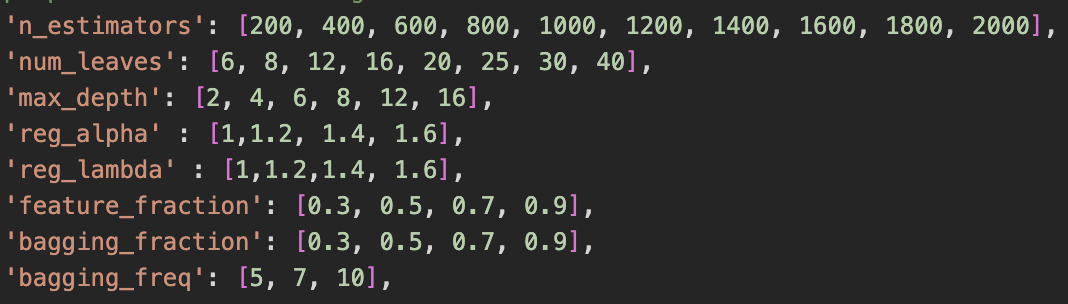
\includegraphics[width=0.9\textwidth]{./plot/ML/RE_RandomSearch.png}
\end{minipage}%
\begin{minipage}{.3\textwidth}
	\centering
	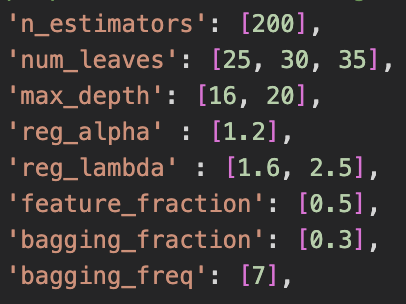
\includegraphics[width=0.9\textwidth]{./plot/ML/RE_GridSearch.png}
\end{minipage}
    \caption{Parameter ranges for Random and Grid Search}
    \label{fig:re_hpsearch}
\end{figure}

\begin{table}[H]
\centering
\begin{tabular}{lrr}\toprule
\textbf{Hyperparameter}                                & \textbf{Random Search} & \textbf{Grid Search} \\\midrule
Number of trees in Random Forest                       & 200                                & 200                              \\
Number of leaves                                       & 25                                 & 30                               \\
Maximum depth of tree                                  & 16                                 & 16                               \\
L1 regularization term on weights                      & 1                                  & 1,2                              \\
L2 regularization term on weights                      & 1,6                                & 1,8                              \\
Fraction of features to be used in each boosting round & 0,5                                & 0,5                              \\
Fraction of data to be used in each boosting round     & 0,3                                & 0,3                              \\
Frequency for bagging                                  & 7                                  & 7                               \\\bottomrule
\end{tabular}
\caption{Best Parameter Settings of Random and Grid Search}
\label{tab:best_rand_grid}
\end{table}

\begin{figure}[H]
	\centering
	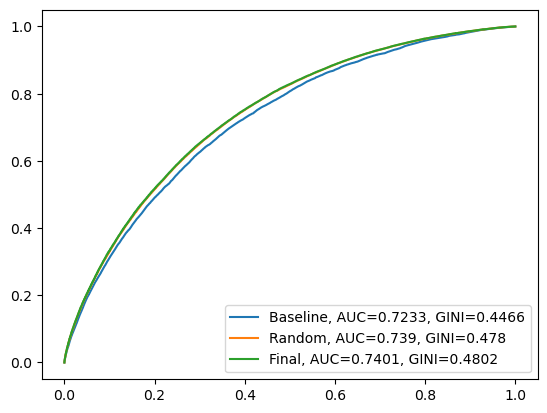
\includegraphics[width=0.65\textwidth]{./plot/ML/ROC_HyperParTuning.png}
    \caption{Performance comparison for Hyperparameter Tuning}
    \label{fig:re_rochp}
\end{figure}

\section{Validation and Comparison}
\label{sec:comp_model}

\subsection{Discriminatory power}
Both models' performance is evaluated using the test and an out-of-time data set. To detect potential overfitting, performance metrics for the training sample are also provided. The Gini values are presented in Table \ref{re_ginicomp} and visually represented in Figure \ref{fig:re_roc1} - \ref{fig:re_roc2}. The Random Forest model exhibits a slightly higher performance in the training and test samples with a relative improvement of about 1,7\%, while the logistic regression model shows a slight advantage in the validation sample with 1,6\% relative difference. Notably, both models demonstrate higher Gini values on the validation sample, indicating no signs of overfitting.

\begin{table}[H]
\centering
\begin{tabular}{lrrrr}\toprule
\textbf{Sample} & \textbf{Logistic Model} & \textbf{Random Forest} & \textbf{abs. Change} & \textbf{rel. Change}\\\midrule
Training   & 0,4626 & 0,4708 & 0,82\%  & 1,77\%  \\
Test       & 0,4638 & 0,4718 & 0,80\%  & 1,72\%  \\
Validation & 0,4810 & 0,4734 & -0,76\% & -1,58\% \\\bottomrule
\end{tabular}
\caption{Comparison of Gini values in training, test and validation sample}
\label{re_ginicomp}
\end{table}

\begin{figure}[H]
\begin{minipage}{.5\textwidth}
	\centering
	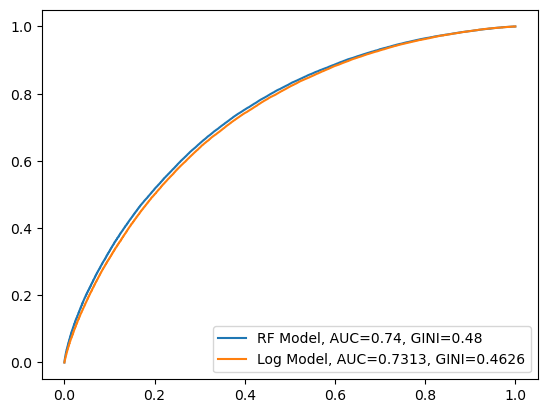
\includegraphics[width=0.9\textwidth]{./plot/ML/ROC_Comp_Train.png}
\end{minipage}%
\begin{minipage}{.5\textwidth}
	\centering
	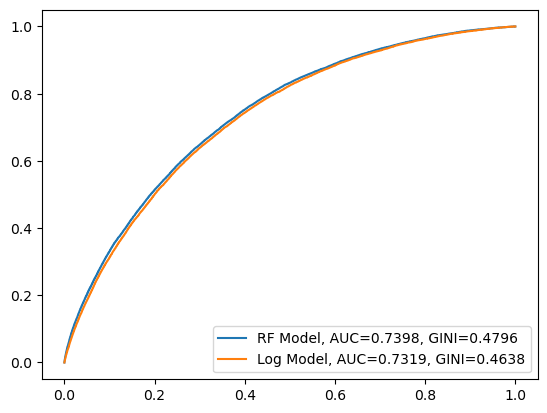
\includegraphics[width=0.9\textwidth]{./plot/ML/ROC_Comp_Test.png}
\end{minipage}
    \caption{AUC comparison in training and test sample}
    \label{fig:re_roc1}
\end{figure}

\begin{figure}[H]
	\centering
	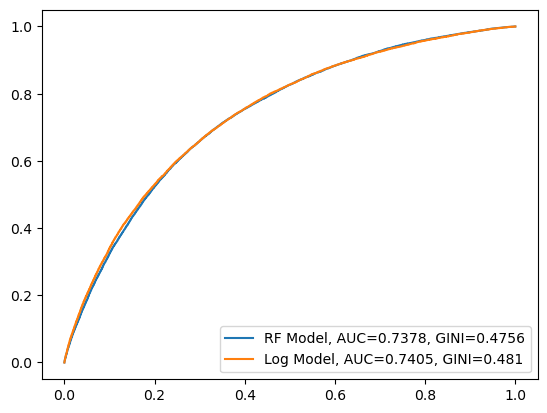
\includegraphics[width=0.65\textwidth]{./plot/ML/ROC_Comp_Validation.png}
    \caption{AUC comparison in Validation sample}
    %\label{fig:re_wholesample}
    \label{fig:re_roc2}
\end{figure}

\subsection{Classification}
To determine an optimal threshold to set a predicted default flag derived from the predicted PD, the F1-score is computed for different values. These values are detailed in Table \ref{tab:re_f1thresh}, leading to the decision to set the threshold with the maximum F1-score at PD > 4\% for both models. The Random Forest model exhibits a slightly higher accuracy with a relative improvement of 11,08\%. The resulting confusion matrices for the training, test and validation samples are visualized in Figure \ref{fig:re_confmatr1} to \ref{fig:re_confmatr3}. On the x-axis, the predicted values are presented, while the y-axis represents true values. Focusing on the most critical cases, where default events are misclassified as non-default (lower left corner), the Random Forest model performs slightly worse in this regard compared to the logistic regression model on all samples.

\begin{table}[H]
\centering
\begin{tabular}{ccc}\toprule
								    & \multicolumn{2}{c}{\textbf{F1-Score}}                 \\\midrule
 \textbf{Threshold}                 & \textbf{Logistic Regression} & \textbf{Random Forest} \\
0,005                               & 0,0362                       & 0,0299                 \\
0,010                               & 0,0464                       & 0,0360                 \\
0,015                               & 0,0561                       & 0,0521                 \\
0,020                               & 0,0648                       & 0,0664                 \\
0,025                               & 0,0721                       & 0,0788                 \\
0,030                               & 0,0777                       & 0,0872                 \\
0,035                               & 0,0819                       & 0,0920                 \\
0,040                               & 0,0836                       & 0,0929                 \\
0,045                               & 0,0830                       & 0,0901                 \\
0,050                               & 0,0803                       & 0,0846                 \\
0,055                               & 0,0751                       & 0,0761                 \\
0,060                               & 0,0687                       & 0,0667                 \\
0,065                               & 0,0608                       & 0,0588                 \\
0,070                               & 0,0522                       & 0,0517                 \\
0,075                               & 0,0438                       & 0,0446                 \\
0,080                               & 0,0362                       & 0,0387                 \\
0,085                               & 0,0290                       & 0,0329                 \\
0,090                               & 0,0234                       & 0,0284                 \\
0,095                               & 0,0193                       & 0,0243                \\\bottomrule
\end{tabular}
\caption{F1 score for different threshold values}
\label{tab:re_f1thresh}
\end{table}

\begin{figure}[H]
\begin{minipage}{.5\textwidth}
	\centering
	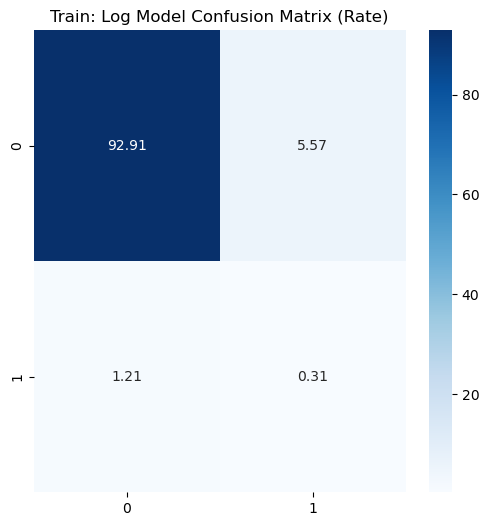
\includegraphics[width=0.9\textwidth]{./plot/ML/ConfMatrix_Train_Log.png}
\end{minipage}%
\begin{minipage}{.5\textwidth}
	\centering
	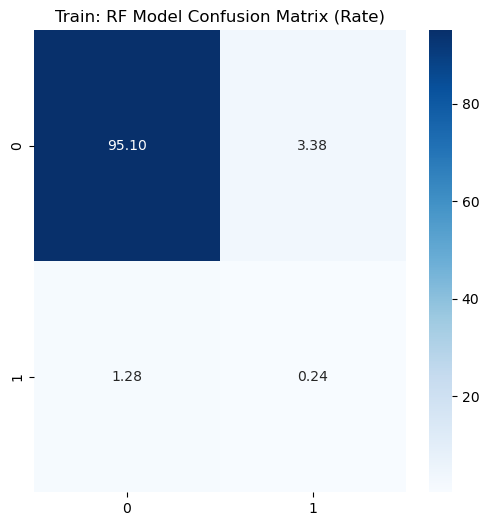
\includegraphics[width=0.9\textwidth]{./plot/ML/ConfMatrix_Train_RF.png}
\end{minipage}
    \caption{Confusionmatrix in training sample}
    \label{fig:re_confmatr1}
\end{figure}
\begin{figure}[H]
\begin{minipage}{.5\textwidth}
	\centering
	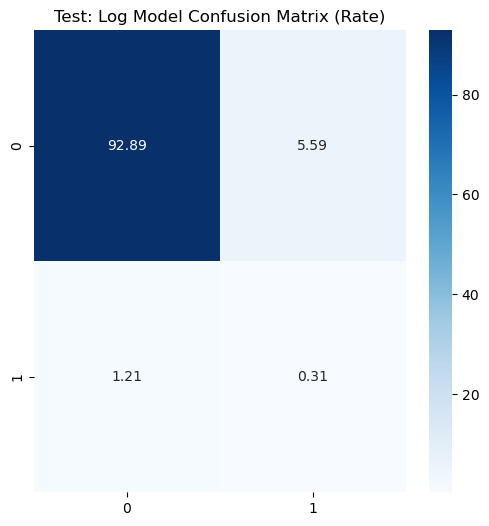
\includegraphics[width=0.9\textwidth]{./plot/ML/ConfMatrix_Test_Log.png}
\end{minipage}%
\begin{minipage}{.5\textwidth}
	\centering
	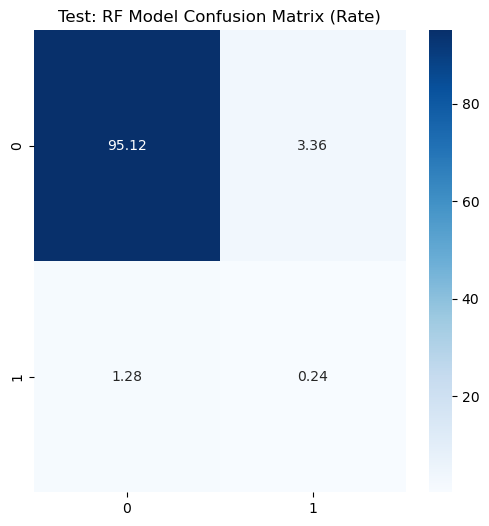
\includegraphics[width=0.9\textwidth]{./plot/ML/ConfMatrix_Test_RF.png}
\end{minipage}
    \caption{Confusionmatrix in test sample}
    %\label{fig:dp_iqr_boxpl}
\end{figure}
\begin{figure}[H]
\begin{minipage}{.5\textwidth}
	\centering
	\includegraphics[width=0.9\textwidth]{./plot/ML/ConfMatrix_Val_Log.png}
\end{minipage}%
\begin{minipage}{.5\textwidth}
	\centering
	\includegraphics[width=0.9\textwidth]{./plot/ML/ConfMatrix_Val_RF.png}
\end{minipage}
    \caption{Confusionmatrix in validation sample}
    \label{fig:re_confmatr3}
\end{figure}

\subsection{Stability Test}
A stability test for both models was conducted by assessing the Gini coefficient on the test and validation samples for each year, as detailed in Table \ref{tab:re_stab} and illustrated through ROC curves in Figure \ref{fig:re_rocstab}. The left side of the Figure is the logistic regression model, while the right side showcases the Random Forest model. Both models exhibited their lowest performance in 2019. The logistic regression model demonstrated its peak discriminatory power in 2018, whereas the Random Forest model excelled in the year 2020. Across the years, both models exhibit a Gini difference of up to 8,4\%, suggesting a moderate level of stability.

\begin{table}[H]
\centering
\begin{tabular}{ccc}\toprule
\textbf{Year} & \textbf{LOG Model} & \textbf{RF Model} \\\midrule
2018          & 0,5202             & 0,5044            \\
2019          & 0,4358             & 0,4440            \\
2020          & 0,4936             & 0,5162            \\
2021          & 0,4810             & 0,4734        	\\\bottomrule   
\end{tabular}
\caption{Stability test over time}
\label{tab:re_stab}
\end{table}

\begin{figure}[H]
\begin{minipage}{.5\textwidth}
	\centering
	\includegraphics[width=0.9\textwidth]{./Stability_LOG.png}
\end{minipage}%
\begin{minipage}{.5\textwidth}
	\centering
	\includegraphics[width=0.9\textwidth]{./Stability_RF.png}
\end{minipage}
    \caption{ROC curve of stability test over time}
    \label{fig:re_rocstab}
\end{figure}

\subsection{Binning Process}
A binning process was executed to provide an overview of the distribution of PDs and default rates. In real-world applications, it is a standard practice to categorize PD values into distinct rating bands, distinguishing between investment and non-investment grades. A straightforward method involves employing fixed ranges for each grade. The specific ranges and the resulting distribution are detailed in Table \ref{tab:re_distrDR} and visually presented in Figure \ref{fig:re_distrDR}. These arbitrarily defined ranges already provide a satisfactory distribution, accompanied by a desired upward trend in defaults. The logistic regression model tends to allocate a greater number of customers with PD values below 0,5\% compared to the Random Forest model. The Random Forest model exhibits a moderate concentration in the range of 1\% to 1,5\%.

\begin{table}[H]
\centering
\begin{tabular}{lrrrrrr}\toprule
\textbf{}        & \multicolumn{2}{c}{\textbf{\# Observation}}                                    & \multicolumn{2}{c}{\textbf{\% Observation}}                                    & \multicolumn{2}{c}{\textbf{\% Default Rate}}                                   \\
\textbf{Range}   & \multicolumn{1}{l}{\textbf{Log}} & \multicolumn{1}{l}{\textbf{RF}} & \multicolumn{1}{l}{\textbf{Log}} & \multicolumn{1}{l}{\textbf{RF}} & \multicolumn{1}{l}{\textbf{Log}} & \multicolumn{1}{l}{\textbf{RF}} \\\midrule
(-inf, 0.001)    & 48.096                                 &                                       & 1\%                                    &                                       & 0,06\%                                 &                                       \\
{[}0.001, 0.005) & 1.665.964                              &                                       & 21\%                                   &                                       & 0,19\%                                 &                                       \\
{[}0.005, 0.01)  & 1.983.432                              & 1.734.463                             & 25\%                                   & 22\%                                  & 0,43\%                                 & 0,17\%                                \\
{[}0.01, 0.015)  & 1.326.997                              & 2.829.949                             & 17\%                                   & 36\%                                  & 0,75\%                                 & 0,48\%                                \\
{[}0.015, 0.02)  & 891.664                                & 1.454.260                             & 11\%                                   & 18\%                                  & 1,09\%                                 & 1,02\%                                \\
{[}0.02, 0.03)   & 1.031.273                              & 1.225.736                             & 13\%                                   & 15\%                                  & 1,58\%                                 & 1,74\%                                \\
{[}0.03, 0.04)   & 493.678                                & 388.029                               & 6\%                                    & 5\%                                   & 2,24\%                                 & 2,65\%                                \\
{[}0.04, inf)    & 470.193                                & 278.860                               & 6\%                                    & 4\%                                   & 3,32\%                                 & 4,06\%        \\\bottomrule                       
\end{tabular}
\caption{Distribution Table of PDs and Default Rates for Logistic Regression and Random Forest Model}
\label{tab:re_distrDR}
\end{table}


\begin{figure}[H]
	\centering
	\includegraphics[width=0.9\textwidth]{./plot/ML/RatingGrades.png}
    \caption{Distribution Plot of PDs and Default Rates for Logistic Regression and Random Forest Model}
    %\label{fig:re_wholesample}
    \label{fig:re_distrDR}
\end{figure}

\section{Interpretability}

\subsection{Global Interpretation}
To interpret the Random Forest model, several techniques described in Chapter \ref{sec:interpret} were utilized. Figure \ref{fig:re_featureimp_split} shows the feature importance by split, signifying the frequency with which a variable is employed for a split. Meanwhile, Figure \ref{fig:re_featureimp_gain} depicts feature importance by gain, denoting the information gain derived from the risk factor during a split. Reiterating the findings of the logistic regression model, the most important risk factors in the Random Forest model are \emph{Credit Score} (fico), \emph{UPB}, \emph{CLTV}, \emph{DTI} and \emph{No Borrowers} (cnt\_borr) as well. The \emph{LTV} was removed from the logistic regression model due to its high correlation with the risk factor \emph{CLTV}. 


\begin{figure}[H]
	\centering
	\includegraphics[width=\textwidth]{./plot/ML/FeatureImportanceSplit.png}
    \caption{Feature Importance by Split}
    \label{fig:re_featureimp_split}
\end{figure}

\begin{figure}[H]
	\centering
	\includegraphics[width=\textwidth]{./plot/ML/FeatureImportanceGain.png}
    \caption{Feature Importance by Gain}
    \label{fig:re_featureimp_gain}
\end{figure}

\subsection{Local Interpretation}
Two particular instances were selected for the \ac{LIME} technique. The first observation received nearly identical PDs of 1,2547\% in both models, while the second observation received vastly different PDs of 59,0619\% in the Logit Model and 2,2576\% in the Random Forest Model. The score composition for the former is displayed in Table \ref{tab:re_PDres} and the \ac{LIME} results are visible in Figures \ref{fig:re_LIMEres_min} and \ref{fig:re_LIMEres_max}. The green bars indicate the features contributing to predicting the "non-default" class and the red bars signify the contribution to the "default" class. 

While the high Credit Score mainly influences the low PD in observation 1 for both models, the lower Credit Score, as well as the higher DTI, resulted in a higher PD in the Logit model. Surprisingly, in the Random Forest model, both features contribute to the classification of "non-default", contrasting the result seen in the first observation.

\begin{table}[H]
\centering
\begin{tabular}{l|rrr|rrr}\toprule
\textbf{}                              & \multicolumn{3}{c}{\textbf{Observation 1}}                                                                                                                                                                        & \multicolumn{3}{c}{\textbf{Observation 2}}                                                                                                                                                                       \\
\multicolumn{1}{l|}{\textbf{Variable}} & \multicolumn{1}{c}{\textbf{\begin{tabular}[c]{@{}c@{}}Original\\ Value\end{tabular}}} & \multicolumn{1}{c}{\textbf{\begin{tabular}[c]{@{}c@{}}Scaled\\ Value\end{tabular}}} & \multicolumn{1}{c|}{\textbf{Score}} & \multicolumn{1}{c}{\textbf{\begin{tabular}[c]{@{}c@{}}Original\\ Value\end{tabular}}} & \multicolumn{1}{c}{\textbf{\begin{tabular}[c]{@{}c@{}}Scaled\\ Value\end{tabular}}} & \multicolumn{1}{c}{\textbf{Score}} \\\midrule
\multicolumn{1}{l|}{Intercept}         &                                                                                       &                                                                                     & \multicolumn{1}{r|}{-4,5457}        &                                                                                       &                                                                                     & -4,5457                            \\
\multicolumn{1}{l|}{Credit Score (fico)}      & 691                                                                                   & -           1,4100                                                                  & \multicolumn{1}{r|}{0,7642}         & 309                                                                                   & -        10,1100                                                                    & 5,4796                             \\
\multicolumn{1}{l|}{DTI (dti)}               & 29,99                                                                                 & -           0,4421                                                                  & \multicolumn{1}{r|}{-0,1802}        & 40,01                                                                                 & 0,5910                                                                              & 0,2409                             \\
\multicolumn{1}{l|}{CLTV (cltv)}              & 73,00                                                                                 & -           0,0359                                                                  & \multicolumn{1}{r|}{-0,0094}        & 30,00                                                                                 & -           2,5257                                                                  & -0,6600                            \\
\multicolumn{1}{l|}{No Borrowers (cnt\_borr)}      & 2                                                                                     & 0,9969                                                                              & \multicolumn{1}{r|}{-0,2476}        & 1                                                                                     & -           0,9326                                                                  & 0,2317                             \\
\multicolumn{1}{l|}{UPB (orig\_upb)}               & 200.000                                                                               & -           0,4313                                                                  & \multicolumn{1}{r|}{-0,1469}        & 110.000                                                                               & -           1,1133                                                                  & -0,3793                            \\
\multicolumn{1}{l|}{Model Score}       & \multicolumn{3}{c|}{-4,3656}                                                                                                                                                                                      & \multicolumn{3}{c}{0,3672}                                                                                                                                                                                       \\
\multicolumn{1}{l|}{PD}                & \multicolumn{3}{c|}{1,25\%}                                                                                                                                                                                       & \multicolumn{3}{c}{59,08\%} \\\bottomrule                                                                                                                                                                                     
\end{tabular}
\caption{PD Result of Logistic Regression model}
\label{tab:re_PDres}
\end{table}

\begin{figure}[H]
	\centering
	\includegraphics[width=0.9\textwidth]{./plot/ML/LIME_minDiff.png}
    \caption{LIME Result of Random Forest, minimum difference in PD}
    \label{fig:re_LIMEres_min}
\end{figure}

\begin{figure}[H]
	\centering
	\includegraphics[width=0.9\textwidth]{./plot/ML/LIME_maxDiff.png}
    \caption{LIME Result of Random Forest, maximum difference in PD}
    \label{fig:re_LIMEres_max}
\end{figure}

\subsection{Individual Decision Trees, PDP and ICE plots}
Two individual decision trees from the Random Forest model are presented in Figure \ref{fig:re_indtree1} and \ref{fig:re_indtree2}. Analyzing the split conditions, they reaffirm the importance of \emph{Credit Score}, \emph{UPB}, \emph{DTI} and \emph{LTV} as primary variables. To assess their influence, Partial Dependence plots of these four features, along with \emph{Prop Val Method = Full Appraisal} and \emph{Loan Purpose = Refinance - Cash Out} are showcased in Figures \ref{fig:pdp_1} to \ref{fig:pdp_2}. All plots are in Appendix \ref{sec:PDP_all}. The observed trends align with the economic rationale: increasing Credit Score corresponds to decreasing PD, while rising \emph{UPB}, \emph{DTI} and \emph{CLTV} are associated with higher PD. Both categorical variables indicate a higher PD if the condition is fulfilled. Individual Conditional Expectation (ICE) plots were generated to further analyze the impact of the four most crucial features \emph{Credit Score}, \emph{UPB}, \emph{CLTV} and \emph{DTI}. Figure \ref{fig:ice_1} to \ref{fig:ice_2} provide a granular analysis of each feature's influence on individual predictions. The findings from these ICE plots also align with the anticipated relationship between the respective risk factor and the PD estimation.

\begin{figure}[H]
	\centering
	\includegraphics[width=0.9\textwidth]{./plot/ML/IndDecTree1.png}
    \caption{Individual Decision Tree 1 of Random Forest}
    %\label{fig:re_wholesample}
    \label{fig:re_indtree1}
\end{figure}

\begin{figure}[H]
	\centering
	\includegraphics[width=0.9\textwidth]{./plot/ML/IndDecTree2.png}
    \caption{Individual Decision Tree 2 of Random Forest}
    %\label{fig:re_wholesample}
    \label{fig:re_indtree2}
\end{figure}

\begin{figure}[H]
\begin{minipage}{.5\textwidth}
	\centering
	\includegraphics[width=0.9\textwidth]{./plot/ML/PDP_fico.png}
\end{minipage}%
\begin{minipage}{.5\textwidth}
	\centering
	\includegraphics[width=0.9\textwidth]{./plot/ML/PDP_orig_upb.png}
\end{minipage}
    \caption{Partial Dependence Plots for Credit score and UPB}
    \label{fig:pdp_1}
\end{figure}

\begin{figure}[H]
\begin{minipage}{.5\textwidth}
	\centering
	\includegraphics[width=0.9\textwidth]{./plot/ML/PDP_cltv.png}
\end{minipage}%
\begin{minipage}{.5\textwidth}
	\centering
	\includegraphics[width=0.9\textwidth]{./plot/ML/PDP_dti.png}
\end{minipage}
    \caption{Partial Dependence Plots for CLTV and DTI}
    %\label{fig:dp_iqr_boxpl}
\end{figure}

\begin{figure}[H]
\begin{minipage}{.5\textwidth}
	\centering
	\includegraphics[width=0.9\textwidth]{./plot/ML/PDP_cd_ppty_val_type__2.png}
\end{minipage}%
\begin{minipage}{.5\textwidth}
	\centering
	\includegraphics[width=0.9\textwidth]{./plot/ML/PDP_loan_purpose__C.png}
\end{minipage}
    \caption{Partial Dependence Plots for Prop Val Method = Full Appraisal and Loan Purpose = Refinance - Cash Out}
    \label{fig:pdp_2}
\end{figure}

\begin{figure}[H]
\begin{minipage}{.5\textwidth}
	\centering
	\includegraphics[width=0.9\textwidth]{./plot/ML/ICE_fico.png}
\end{minipage}%
\begin{minipage}{.5\textwidth}
	\centering
	\includegraphics[width=0.9\textwidth]{./plot/ML/ICE_orig_upb.png}
\end{minipage}
    \caption{Individual Conditional Expectation Plots for Credit Score and UPB}
    \label{fig:ice_1}
\end{figure}

\begin{figure}[H]
\begin{minipage}{.5\textwidth}
	\centering
	\includegraphics[width=0.9\textwidth]{./plot/ML/ICE_cltv.png}
\end{minipage}%
\begin{minipage}{.5\textwidth}
	\centering
	\includegraphics[width=0.9\textwidth]{./plot/ML/ICE_dti.png}
\end{minipage}
    \caption{Individual Conditional Expectation Plots for CLTV and DTI}
    \label{fig:ice_2}
\end{figure}


\chapter{Conclusio}

\appendix
\chapter{Dunno Man}
\section{Erster Section}
	\subsection{Erster ding}
blabla hier Text


\newpage
\bibliography{Literature}

\end{document}
